\documentclass[Master, ngerman, UKenglish]{scrbook}
%------------------------------------------------------------------------------
% This file contains a skeleton thesis for
% a Physics or Astronomy Institute in the University of Bonn.

% Specify the thesis type as an option: PhD, Master, Diplom, Bachelor.
% Specify the thesis stage as an option: Draft (default), Submit, Final, PILibrary.

% Specify the language(s) in the class and then use babel.
% If you need more than one language, give the default language last,
% e.g. ngerman, UKenglish for a thesis in British (UK) English where you want
% to be able to set the language to German for some part of it.

%------------------------------------------------------------------------------
% Pass TeX Live version to the package.
% Use command pdflatex --version to find out which version you are running.
% twoside=true is suitable for printing, while twoside=false is probably better for PDF version.
\usepackage[twoside=true, texlive=2017, astrobib]{ubonn-thesis}

%------------------------------------------------------------------------------
% Adjustments to standard biblatex style.
% Change option to backref=false when your thesis is ready to turn off back-referencing.
% Pass the option showurl=false to shorten your bibliography by not including url fields.
% Astronomy theses usually set block=none.
\usepackage[backref=true, block=none]{ubonn-biblatex}

%------------------------------------------------------------------------------
% Glossary package
% \usepackage[acronym,toc,nosuper]{glossaries}
% TikZ packages and libraries
% \usepackage{tikz}
% \usepackage{tikz-3dplot}
% \usepackage{pgfplots}
% \usetikzlibrary{positioning,shapes,arrows}
% \usetikzlibrary{decorations.pathmorphing}
% \usetikzlibrary{decorations.markings}
\usepackage{thesis_defs}

%------------------------------------------------------------------------------
% Instead of colouring  links, cites, table of contents etc.
% put them in a coloured box for the screen version.
% This is probably a good idea when you print your thesis.
% \hypersetup{colorlinks=false,
%   linkbordercolor=blue,citebordercolor=magenta,urlbordercolor=darkgreen
% }

%------------------------------------------------------------------------------
% When writing your thesis it is often helpful to have the date and
% time in the output file. Comment this out for the final version.
\ifoot[\today{} \thistime]{\today{} \thistime}

% In order to check if your labels are referenced try the refcheck package
% \usepackage{refcheck}

%------------------------------------------------------------------------------
% biblatex is included by ubonn-thesis. Look there for the settings used.
% See the options for settings that can be changed easily.
% For further changes copy the \RequirePackage[...]{biblatex} here
% and include ubonn-thesis with the option biblatex=false.

% Specify the bibliography files here and not at the end!
% Use standard_refs-bibtex if you use bibtex or bibtex8
% and standard_refs-biber  if you use biber
\addbibresource{bib/thesis_refs.bib}
\addbibresource{bib/standard_refs-biber.bib}

%------------------------------------------------------------------------------
% The following definitions are used to produce the title pages
% needed at various stages
\newcommand{\thesistitle}{Title of the Thesis}
\newcommand*{\thesisauthor}{Author's name}
\newcommand*{\thesistown}{Place of birth}
\renewcommand*{\InstituteName}{\AIFA}
\renewcommand*{\inInstitute}{\inAIFA}
\renewcommand*{\InstituteAddress}{\PIaddress}
% Adjust \thesisreferee...text depending on male/female referee
\newcommand*{\thesisrefereeonetext}{1.\ Gutachter}
\newcommand*{\thesisrefereeone}{Prof.\ Dr.\ John Smith}
\newcommand*{\thesisrefereetwotext}{2.\ Gutachterin}
\newcommand*{\thesisrefereetwo}{Prof.\ Dr.\ Anne Jones}
% Date when thesis was submitted (Master/Diplom)
% Year or Month, Year when thesis was submitted (PhD)
\newcommand*{\thesissubmit}{XX.YY.2021}
% \newcommand*{\thesissubmit}{Month 2021}
% Date of thesis examination (PhD)
\newcommand*{\thesispromotion}{XX.YY.2021}
% Month and year of the final printed version of the thesis
\newcommand*{\thesismonth}{MMM}
\newcommand*{\thesisyear}{2021}
\newcommand*{\thesisnumber}{BONN-IR-2021-XXX}
% Dedication
% \newcommand*{\thesisdedication}{}

%------------------------------------------------------------------------------
% The abstract is only needed for the printed version and should be in
% English regardless of the language of the thesis
\newcommand{\thesisabstract}{%
  \begin{otherlanguage}{UKenglish}
    This is your thesis abstract. It may be in a language that is
    different from the rest of your thesis.
  \end{otherlanguage}
}

%------------------------------------------------------------------------------
% \includeonly can be used to select which chapters you want to process
% A simple \include command just inserts a \clearpage before and after the file
% Note that \includeonly can be quite picky! Do not forget to put a
% comma after the filename, otherwise it will simply be ignored!
% \includeonly{%
%   thesis_intro,
%   thesis_appendix,
%   thesis_acknowledge
% }

%------------------------------------------------------------------------------
% Give a list of directories where figures can be found. Do not leave
% any spaces in the list and end the directory name with a /
\graphicspath{%
  {figs/}%
  {figs/cover/}%
}

%------------------------------------------------------------------------------
% Make a glossary and a list of acronyms
% \makeglossaries

% Glossary entries
% \input{thesis_glossary}

% Draft version - add the word DRAFT on the cover pages
\ifthenelse{\equal{\ThesisVersion}{Draft}}{%
  \usepackage{background}
  \backgroundsetup{contents=DRAFT, color=blue!30}
}

%------------------------------------------------------------------------------
\begin{document}

% Make cover and title pages
\makethesistitle

\pagestyle{scrplain}

%------------------------------------------------------------------------------
% You can add your acknowledgements here - don't forget to also add
% them to \includeonly above
%------------------------------------------------------------------------------
\chapter*{Acknowledgements}
\label{sec:ack}
%------------------------------------------------------------------------------

I would like to thank first and foremost my supervisors Prof. Dr. Stefan Krieg and Prof. Dr. Thomas Luu who introduced me into the field of Computational Physics. They gave me the incredible opportunity to work with them at Forschungszentrum Jülich on this project. 

I am extremely grateful to Dr. Evan Berkowitz, with whom I was closely working. His guidance and continuous support helped me throughout my master's thesis. I am also grateful for the excellent notes that Evan provided, which laid the groundwork for my thesis.

Special thanks to my colleagues Keshvi, Christoph, Johann, Nico, and Marcel for the ideas and suggestions in the meetings throughout the year. Especially Aleksandra Salkina who supported me throughout my whole Master's study. I also sincerely acknowledge the computing time granted through JARA on the supercomputer JURECA at Forschungszentrum Jülich.

% You should probably use \texttt{\textbackslash chapter*} for
% acknowledgements at the beginning of a thesis and
% \texttt{\textbackslash chapter} for the end.

%%% Local Variables: 
%%% mode: latex
%%% TeX-master: "../mythesis"
%%% End: 


\tableofcontents

\mainmatter
\pagestyle{scrheadings}

% Turn off DRAFT for the following pages
\ifthenelse{\equal{\ThesisVersion}{Draft}}{%
  \backgroundsetup{contents={}}
}{}

%------------------------------------------------------------------------------
% Add your chapters here - don't forget to also add them to \includeonly above
% !TEX root = mythesis.tex

%==============================================================================
\chapter{Introduction}
\label{sec:intro}
%==============================================================================

Ever since the discovery of graphene in 2004, scientists have tried to examine the properties of this new material. One direction of study are the excitonic insulators which were theorized to be emerging in these carbon nanostructures. The excitons have similarities with Cooper pairs, which are responsible for the superconductivity in materials, however excitons do not transfer charge. Physicists are nevertheless intrigued to study the properties of the bosonic-like particles. The properties of excitonic bound states can be used for the development of new-age devices, i.e., for the development of topologically protected qubits, switching devices, and in heat exchangers.

Density functional theory (DFT) is the most widely used approach to tackle many-body problems in material science. It uses an accurate approximation of the exchange-correlation for the electron system. Another approach is, to use Monte Carlo (MC) methods, and more precisely the Hybrid Monte Carlo (HMC) algorithm, which can be directly applied to the Hamiltonian of the theory. Despite being the most used algorithm in modern lattice  QCD simulations, it has been rarely used in condensed matter.

The goal of this thesis is to estimate the ground binding energy of the exciton in graphene. We will apply the HMC algorithm on the Hubbard model in order to find the correlation functions, representing the exciton and its free constituents. The simulation will be done on a bipartite hexagonal lattice which is a model of the real carbon mono-layered sheets. From the acquired correlators, we will be able to extract the binding energy of the quasi-particle. As the results are simulation dependent, we will try to find the temporal continuum limit and the infinite volume limit, so that the final results are independent of any discretization.

The layout of thesis is organized as follows. In \cref{sec:theory}, we introduce the relevant theoretical background, including the definition of the exciton, an introduction to the Hubbard model, and the sought observables. We describe in \cref{sec:methods} the methods used for simulating the observables and extracting their binding energies, followed by an explanation in \cref{sec:symmetries} of the symmetries of the system and theory that will allow us to make our results more precise. In \cref{sec:excitons}, we first show an algorithm that generates one- and two-body correlation functions. Then we analyze the data and present the results for the binding energy. Finally, we discuss in \cref{sec:conclusion} the results and outline a possible further research. There are additional results and detailed derivations provided in \cref{sec:app}, which are too large to be put in without interrupting the flow of the previous chapters.

% The introduction usually gives a few pages of introduction to the
% whole subject, maybe even starting with the Greeks.

% For more information on \LaTeX{} and the packages that are available
% see for example the books of Kopka%~\cite{kopka04}
%  and Goossens et
% al%~\cite{goossens04}.

% A lot of useful information on particle physics can be found in the
% \enquote{Particle Data Book}%~\cite{pdg2010}.

% I have resisted the temptation to put a lot of definitions into the
% file \texttt{thesis\_defs.sty}, as everyone has their own taste as
% to what scheme they want to use for names.
% However, a few examples are included to help you get started:
% \begin{itemize}
% \setlength{\itemsep}{0pt}\setlength{\parskip}{0pt}
% \item cross-sections are measured in \si{\pb} and integrated
%   luminosity in \si{\invpb};
% \item the \KoS is an interesting particle;
% \item the missing transverse momentum, \pTmiss, is often called
%   missing transverse energy, even though it is calculated using a vector sum.
% \end{itemize}
% Note that the examples of units assume that you are using the
% \textsf{siunitx} package.

% It also is probably a good idea to include a few well formatted
% references in the thesis skeleton. More detailed suggestions on what
% citation types to use can be found in the \enquote{Thesis Guide}%~\cite{thesis-guide}:
% \begin{itemize}
% \item articles in refereed journals%~\cite{pdg2010,Aad:2010ey};
% \item a book%~\cite{Halzen:1984mc};
% \item a PhD thesis%~\cite{tlodd:2012} and a Diplom thesis~\cite{mergelmeyer:2011};
% \item a collection of articles%~\cite{lhc:vol1};
% \item a conference note%~\cite{ATLAS-CONF-2011-008};
% \item a preprint%~\cite{atlas:perf:2009} 
% (you can also use
%   \texttt{@online} or \texttt{@booklet} for such things);
% \item something that is only available online%~\cite{thesis-guide}.
% \end{itemize}

% At the end of the introduction it is normal to say briefly what comes
% in the following chapters.

% The line at the beginning of this file is used by TeXstudio etc.\ to
% specify which is the master \LaTeX\ file, so that you can compile your thesis
% directly from this file.
% If your thesis is called something other than \texttt{mythesis}, adjust it as appropriate.

% Use this command inside the file or change \include to \input
% if you do not want the references on a separate page.
\printbibliography[heading=subbibliography]

%------------------------------------------------------------------------------
% Use biblatex for the bibliography.
% Add bibliography to Table of Contents.
% Use this command  (and remove refsection environments)
% to print all references at the end of the thesis.
% \printbibliography[heading=bibintoc]

%------------------------------------------------------------------------------
\appendix
% \part*{Appendix}
% Add your appendices here - don't forget to also add them to \includeonly above
%------------------------------------------------------------------------------
\chapter{Appendix}
\label{sec:app}
%------------------------------------------------------------------------------

\section{Symmetry Correlation Functions}
We will derive in detail how the symmetry operators transform the two-body correlation functions. In this work we are working with only two kinds of correlators, but from them we can also get a feeling of the symmetry transformations. As a side note, it is shown on the right side of the column sign (":") in the titles if the operator transforms well the full Hamiltonian or only at half-filling.

\subsection{Particle-Hole Correlation Function}

Since we have already shown in \cref{ssec:sym-twobody} the transformation of \cref{eq:phhpmat} using the thermal trace cyclicity property, we will directly start from the next symmetry operator.

\subsubsection{\underline{$I : H - \vec{\mu}\cdot\vec{q}$}}

\begin{equation}
  \begin{aligned}
    C_{Q=0,S=1,S^3=-1;k,q,r,s} \\
    =& \frac{1}{Z}tr\left[p_kh_qe^{-H\tau}h^\dagger_rp^\dagger_se^{-H\left(\beta-\tau\right)}\right] \\
    =& \frac{1}{Z}tr\left[I^{-1}Ip_kI^{-1}Ih_qI^{-1}Ie^{-H\tau}I^{-1}Ih^\dagger_rI^{-1}Ip^\dagger_sI^{-1}Ie^{-H\left(\beta-\tau\right)}\right] \\
    =& \frac{1}{Z}tr\left[Ip_kI^{-1}Ih_qI^{-1}Ie^{-H\tau}I^{-1}Ih^\dagger_rI^{-1}Ip^\dagger_sI^{-1}Ie^{-H\left(\beta-\tau\right)I^{-1}}\right] \\
    =& \frac{1}{Z}tr\left[(\Sigma h)^\dagger_k(\Sigma p)^\dagger_qe^{-H\tau}(\Sigma p)_r(\Sigma h)_se^{-H\left(\beta-\tau\right)}\right] \\
    =& \frac{1}{Z}tr\left[(\Sigma p)^\dagger_q(\Sigma h)^\dagger_ke^{-H\tau}(\Sigma h)_s(\Sigma p)_re^{-H\left(\beta-\tau\right)}\right] \\
    =& \frac{1}{Z}tr\left[(\Sigma p)_r(\Sigma h)_se^{-H\left(\beta-\tau\right)}(\Sigma h)^\dagger_k(\Sigma p)^\dagger_qe^{-H\tau}\right]
  \end{aligned}
\end{equation}

\renewcommand{\cor}[4]{p_{#1}h_{#2}h^\dagger_{#3}p^\dagger_{#4}}
\newcommand{\dscor}[4]{\left(\Sigma h\right)_{#1}^\dagger \left(\Sigma p\right)_{#2}^\dagger \left(\Sigma p\right)_{#3}\left(\Sigma h\right)_{#4}}
\renewcommand{\dcor}[4]{h_{#1}^\dagger p_{#2}^\dagger p_{#3} h_{#4}}

\begin{equation}
  \begin{aligned}
    &C_{Q=0,S=1,S^3=-1;k,q,r,s} \\
    &= I^{-1} \left[ 
    {\begin{array}{cccc}
      \cor{+}{+}{+}{+} & \cor{+}{+}{+}{-} & \cor{+}{+}{-}{+} & \cor{+}{+}{-}{-} \\
      \cor{+}{-}{+}{+} & \cor{+}{-}{+}{-} & \cor{+}{-}{-}{+} & \cor{+}{-}{-}{-} \\
      \cor{-}{+}{+}{+} & \cor{-}{+}{+}{-} & \cor{-}{+}{-}{+} & \cor{-}{+}{-}{-} \\
      \cor{-}{-}{+}{+} & \cor{-}{-}{+}{-} & \cor{-}{-}{-}{+} & \cor{-}{-}{-}{-} \\
    \end{array} } \right]_{k,q,r,s} (\tau)\:I \\
    &= \left[\resizebox{\textwidth}{!}{
    ${\begin{array}{cccc}
      \dscor{+}{+}{+}{+} & \dscor{+}{+}{+}{-} & \dscor{+}{+}{-}{+} & \dscor{+}{+}{-}{-} \\
      \dscor{+}{-}{+}{+} & \dscor{+}{-}{+}{-} & \dscor{+}{-}{-}{+} & \dscor{+}{-}{-}{-} \\
      \dscor{-}{+}{+}{+} & \dscor{-}{+}{+}{-} & \dscor{-}{+}{-}{+} & \dscor{-}{+}{-}{-} \\
      \dscor{-}{-}{+}{+} & \dscor{-}{-}{+}{-} & \dscor{-}{-}{-}{+} & \dscor{-}{-}{-}{-} \\
    \end{array} }$}
    \right]_{k,q,r,s} (\tau) \\
    &= \left[ 
    {\begin{array}{cccc}
      \dcor{-}{-}{-}{-} & \dcor{-}{-}{-}{+} & \dcor{-}{-}{+}{-} & \dcor{-}{-}{+}{+} \\
      \dcor{-}{+}{-}{-} & \dcor{-}{+}{-}{+} & \dcor{-}{+}{+}{-} & \dcor{-}{+}{+}{+} \\
      \dcor{+}{-}{-}{-} & \dcor{+}{-}{-}{+} & \dcor{+}{-}{+}{-} & \dcor{+}{-}{+}{+} \\
      \dcor{+}{+}{-}{-} & \dcor{+}{+}{-}{+} & \dcor{+}{+}{+}{-} & \dcor{+}{+}{+}{+} \\
    \end{array} } 
    \right]_{k,q,r,s} (\tau) \\
  \end{aligned}
\end{equation}

\renewcommand{\cor}[4]{p_{#3}h_{#4}h^\dagger_{#1}p^\dagger_{#2}}

\begin{equation}
  \begin{aligned}
    &= \left[ 
    {\begin{array}{cccc}
      \cor{-}{-}{-}{-} & \cor{-}{-}{-}{+} & \cor{-}{-}{+}{-} & \cor{-}{-}{+}{+} \\
      \cor{-}{+}{-}{-} & \cor{-}{+}{-}{+} & \cor{-}{+}{+}{-} & \cor{-}{+}{+}{+} \\
      \cor{+}{-}{-}{-} & \cor{+}{-}{-}{+} & \cor{+}{-}{+}{-} & \cor{+}{-}{+}{+} \\
      \cor{+}{+}{-}{-} & \cor{+}{+}{-}{+} & \cor{+}{+}{+}{-} & \cor{+}{+}{+}{+} \\
    \end{array} } 
    \right]_{r,s,k,q} (\beta-\tau) \\
  \end{aligned}
\end{equation}

\renewcommand{\dcor}[4]{p_{#2}^\dagger h_{#1}^\dagger h_{#4} p_{#3}}

\begin{equation}
  \begin{aligned}
    &= \left[ {\begin{array}{cccc}
      \dcor{-}{-}{-}{-} & \dcor{-}{-}{-}{+} & \dcor{-}{-}{+}{-} & \dcor{-}{-}{+}{+} \\
      \dcor{-}{+}{-}{-} & \dcor{-}{+}{-}{+} & \dcor{-}{+}{+}{-} & \dcor{-}{+}{+}{+} \\
      \dcor{+}{-}{-}{-} & \dcor{+}{-}{-}{+} & \dcor{+}{-}{+}{-} & \dcor{+}{-}{+}{+} \\
      \dcor{+}{+}{-}{-} & \dcor{+}{+}{-}{+} & \dcor{+}{+}{+}{-} & \dcor{+}{+}{+}{+} \\
    \end{array} } \right]_{q,k,s,r} (\tau)
  \end{aligned}
\end{equation}
Depending on what transformation we use to get back to $\langle phh^\dagger p^\dagger\rangle$, we get two transformations which are time reverse to one another. We notice the same behavior for all operators.

\begin{equation}
  \begin{aligned}
    C_{Q=0,S=1,S^3=-1;k,q,r,s} (\tau) \\
    =& \left[ {\begin{array}{cc}
      0 & \sigma_1 \\
      \sigma_1 & 0 \\
    \end{array} } \right]
    {C_{Q=0,S=1,S^3=-1;r,s,k,q}}^\top (\beta-\tau)
    \left[ {\begin{array}{cc}
      0 & \sigma_1 \\
      \sigma_1 & 0 \\
    \end{array} } \right]
  \end{aligned}
\end{equation}

\begin{equation}
  \begin{aligned}
    C_{Q=0,S=1,S^3=-1;k,q,r,s} (\tau) \\
    =& \left[ {\begin{array}{cccc}
      1 & 0 & 0 & 0 \\
      0 & 0 & 1 & 0 \\
      0 & 1 & 0 & 0 \\
      0 & 0 & 0 & 1 \\
    \end{array} } \right]
    \left[ {\begin{array}{cc}
      0 & \sigma_1 \\
      \sigma_1 & 0 \\
    \end{array} } \right]
    C_{Q=0,S=1,S^3=+1;q,k,s,r} (\tau)
    \left[ {\begin{array}{cc}
      0 & \sigma_1 \\
      \sigma_1 & 0 \\
    \end{array} } \right]
    \left[ {\begin{array}{cccc}
      1 & 0 & 0 & 0 \\
      0 & 0 & 1 & 0 \\
      0 & 1 & 0 & 0 \\
      0 & 0 & 0 & 1 \\
    \end{array} } \right]
  \end{aligned}
\end{equation}

\subsubsection{\underline{$C : H$}}

\begin{equation}
  \begin{aligned}
    C_{Q=0,S=1,S^3=-1;k,q,r,s} \\
    =& \frac{1}{Z}tr\left[p_kh_qe^{-H\tau}h^\dagger_rp^\dagger_se^{-H\left(\beta-\tau\right)}\right] \\
    =& \frac{1}{Z}tr\left[C^{-1}Cp_kC^{-1}Ch_qC^{-1}Ce^{-H\tau}C^{-1}Ch^\dagger_rC^{-1}Cp^\dagger_sC^{-1}Ce^{-H\left(\beta-\tau\right)}\right] \\
    =& \frac{1}{Z}tr\left[h_kp_qe^{-H\tau}p^\dagger_rh^\dagger_se^{-H\left(\beta-\tau\right)}\right] \\
    =& \frac{1}{Z}tr\left[p_qh_ke^{-H\tau}h^\dagger_sp^\dagger_re^{-H\left(\beta-\tau\right)}\right]
  \end{aligned}
\end{equation}

\renewcommand{\cor}[4]{p_{#1}h_{#2}h^\dagger_{#3}p^\dagger_{#4}}
\renewcommand{\dcor}[4]{p_{#3}^\dagger h_{#4}^\dagger h_{#1} p_{#2}}

\begin{equation}
  \begin{aligned}
    C_{Q=0,S=1,S^3=-1;k,q,r,s} \\
    &= C^{-1} \left[ 
    {\begin{array}{cccc}
      \cor{+}{+}{+}{+} & \cor{+}{+}{+}{-} & \cor{+}{+}{-}{+} & \cor{+}{+}{-}{-} \\
      \cor{+}{-}{+}{+} & \cor{+}{-}{+}{-} & \cor{+}{-}{-}{+} & \cor{+}{-}{-}{-} \\
      \cor{-}{+}{+}{+} & \cor{-}{+}{+}{-} & \cor{-}{+}{-}{+} & \cor{-}{+}{-}{-} \\
      \cor{-}{-}{+}{+} & \cor{-}{-}{+}{-} & \cor{-}{-}{-}{+} & \cor{-}{-}{-}{-} \\
    \end{array} } \right]_{k,q,r,s} (\tau)\:C \\
  \end{aligned}
\end{equation}

\renewcommand{\cor}[4]{h_{#1}p_{#2}p^\dagger_{#3}h^\dagger_{#4}}

\begin{equation}
  \begin{aligned}  
    &=\left[ {\begin{array}{cccc}
      \cor{+}{+}{+}{+} & \cor{+}{+}{+}{-} & \cor{+}{+}{-}{+} & \cor{+}{+}{-}{-} \\
      \cor{+}{-}{+}{+} & \cor{+}{-}{+}{-} & \cor{+}{-}{-}{+} & \cor{+}{-}{-}{-} \\
      \cor{-}{+}{+}{+} & \cor{-}{+}{+}{-} & \cor{-}{+}{-}{+} & \cor{-}{+}{-}{-} \\
      \cor{-}{-}{+}{+} & \cor{-}{-}{+}{-} & \cor{-}{-}{-}{+} & \cor{-}{-}{-}{-} \\
    \end{array} } \right]_{k,q,r,s} (\tau) \\
    &=\left[ 
    {\begin{array}{cccc}
      \dcor{+}{+}{+}{+} & \dcor{+}{+}{+}{-} & \dcor{+}{+}{-}{+} & \dcor{+}{+}{-}{-} \\
      \dcor{+}{-}{+}{+} & \dcor{+}{-}{+}{-} & \dcor{+}{-}{-}{+} & \dcor{+}{-}{-}{-} \\
      \dcor{-}{+}{+}{+} & \dcor{-}{+}{+}{-} & \dcor{-}{+}{-}{+} & \dcor{-}{+}{-}{-} \\
      \dcor{-}{-}{+}{+} & \dcor{-}{-}{+}{-} & \dcor{-}{-}{-}{+} & \dcor{-}{-}{-}{-} \\
    \end{array} } \right]_{r,s,k,q} (\beta-\tau) \\
  \end{aligned}
\end{equation}

\renewcommand{\cor}[4]{p_{#2}h_{#1}h^\dagger_{#4}p^\dagger_{#3}}

\begin{equation}
  \begin{aligned}
    &=\left[ {\begin{array}{cccc}
      \cor{+}{+}{+}{+} & \cor{+}{+}{+}{-} & \cor{+}{+}{-}{+} & \cor{+}{+}{-}{-} \\
      \cor{+}{-}{+}{+} & \cor{+}{-}{+}{-} & \cor{+}{-}{-}{+} & \cor{+}{-}{-}{-} \\
      \cor{-}{+}{+}{+} & \cor{-}{+}{+}{-} & \cor{-}{+}{-}{+} & \cor{-}{+}{-}{-} \\
      \cor{-}{-}{+}{+} & \cor{-}{-}{+}{-} & \cor{-}{-}{-}{+} & \cor{-}{-}{-}{-} \\
    \end{array} } \right]_{q,k,s,r} (\tau)
  \end{aligned}
\end{equation}

\begin{equation}
  C_{Q=0,S=1,S^3=-1;k,q,r,s} (\tau) = {C_{Q=0,S=1,S^3=+1;r,s,k,q}}^\top (\beta-\tau)
\end{equation}

\begin{equation}
  \begin{aligned}
    C_{Q=0,S=1,S^3=-1;k,q,r,s} (\tau) =
    \left[ {\begin{array}{cccc}
      1 & 0 & 0 & 0 \\
      0 & 0 & 1 & 0 \\
      0 & 1 & 0 & 0 \\
      0 & 0 & 0 & 1 \\
    \end{array} } \right]
    C_{Q=0,S=1,S^3=-1;q,k,s,r}(\tau)
    \left[ {\begin{array}{cccc}
      1 & 0 & 0 & 0 \\
      0 & 0 & 1 & 0 \\
      0 & 1 & 0 & 0 \\
      0 & 0 & 0 & 1 \\
    \end{array} } \right]
  \end{aligned}
\end{equation}

\subsubsection{\underline{$XF : H$}}

\begin{equation}
  \resizebox{\textwidth}{!}{%
  $
  \begin{aligned}
    &C_{Q=0,S=1,S^3=-1;k,q,r,s}\\ 
    &= \frac{1}{Z}tr\left[p_kh_qe^{-H\tau}h^\dagger_rp^\dagger_se^{-H\left(\beta-\tau\right)}\right] \\
    &= \frac{1}{Z}tr\left[(XF)^{-1}(XF)p_k(XF)^{-1}(XF)h_q(XF)^{-1}(XF)e^{-H\tau}(XF)^{-1}(XF)h^\dagger_r(XF)^{-1}(XF)p^\dagger_s(XF)^{-1}(XF)e^{-H\left(\beta-\tau\right)}\right] \\
    &= \frac{1}{Z}tr\left[(\Sigma p)^\dagger_k(\Sigma h)^\dagger_qe^{-H\tau}(\Sigma h)_r(\Sigma p)_se^{-H\left(\beta-\tau\right)}\right]
  \end{aligned}$}
\end{equation}

\renewcommand{\cor}[4]{p_{#1}h_{#2}h^\dagger_{#3}p^\dagger_{#4}}
\renewcommand{\dscor}[4]{\left(\Sigma p\right)_{#1}^\dagger \left(\Sigma h\right)_{#2}^\dagger \left(\Sigma h\right)_{#3}\left(\Sigma p\right)_{#4}}
\renewcommand{\dcor}[4]{p_{#1}^\dagger h_{#2}^\dagger h_{#3} p_{#4}}

\begin{equation}
  \begin{aligned}
    &C_{Q=0,S=1,S^3=-1;k,q,r,s} \\
    &=\left(XF\right)^{-1} \left[ 
    {\begin{array}{cccc}
      \cor{+}{+}{+}{+} & \cor{+}{+}{+}{-} & \cor{+}{+}{-}{+} & \cor{+}{+}{-}{-} \\
      \cor{+}{-}{+}{+} & \cor{+}{-}{+}{-} & \cor{+}{-}{-}{+} & \cor{+}{-}{-}{-} \\
      \cor{-}{+}{+}{+} & \cor{-}{+}{+}{-} & \cor{-}{+}{-}{+} & \cor{-}{+}{-}{-} \\
      \cor{-}{-}{+}{+} & \cor{-}{-}{+}{-} & \cor{-}{-}{-}{+} & \cor{-}{-}{-}{-} \\
    \end{array}}
    \right]_{k,q,r,s} (\tau)\:\left(XF\right) \\
    &= \left[\resizebox{\textwidth}{!}{%
    $
    {\begin{array}{cccc}
      \dscor{+}{+}{+}{+} & \dscor{+}{+}{+}{-} & \dscor{+}{+}{-}{+} & \dscor{+}{+}{-}{-} \\
      \dscor{+}{-}{+}{+} & \dscor{+}{-}{+}{-} & \dscor{+}{-}{-}{+} & \dscor{+}{-}{-}{-} \\
      \dscor{-}{+}{+}{+} & \dscor{-}{+}{+}{-} & \dscor{-}{+}{-}{+} & \dscor{-}{+}{-}{-} \\
      \dscor{-}{-}{+}{+} & \dscor{-}{-}{+}{-} & \dscor{-}{-}{-}{+} & \dscor{-}{-}{-}{-} \\
    \end{array}}$}
    \right]_{k,q,r,s} (\tau) \\
    &= \left[ 
    {\begin{array}{cccc}
      \dcor{-}{-}{-}{-} & \dcor{-}{-}{-}{+} & \dcor{-}{-}{+}{-} & \dcor{-}{-}{+}{+} \\
      \dcor{-}{+}{-}{-} & \dcor{-}{+}{-}{+} & \dcor{-}{+}{+}{-} & \dcor{-}{+}{+}{+} \\
      \dcor{+}{-}{-}{-} & \dcor{+}{-}{-}{+} & \dcor{+}{-}{+}{-} & \dcor{+}{-}{+}{+} \\
      \dcor{+}{+}{-}{-} & \dcor{+}{+}{-}{+} & \dcor{+}{+}{+}{-} & \dcor{+}{+}{+}{+} \\
    \end{array} } \right]_{k,q,r,s} (\tau) \\
  \end{aligned}
\end{equation}
  \renewcommand{\cor}[4]{p_{#4}h_{#3}h^\dagger_{#2}p^\dagger_{#1}}
\begin{equation}
  \begin{aligned}    
    &= \left[ 
    {\begin{array}{cccc}
      \cor{-}{-}{-}{-} & \cor{-}{-}{-}{+} & \cor{-}{-}{+}{-} & \cor{-}{-}{+}{+} \\
      \cor{-}{+}{-}{-} & \cor{-}{+}{-}{+} & \cor{-}{+}{+}{-} & \cor{-}{+}{+}{+} \\
      \cor{+}{-}{-}{-} & \cor{+}{-}{-}{+} & \cor{+}{-}{+}{-} & \cor{+}{-}{+}{+} \\
      \cor{+}{+}{-}{-} & \cor{+}{+}{-}{+} & \cor{+}{+}{+}{-} & \cor{+}{+}{+}{+} \\
    \end{array} } \right]_{s,r,k,q} (\beta-\tau)
  \end{aligned}
\end{equation}

\begin{equation}
  \begin{aligned}
    C_{Q=0,S=1,S^3=-1;k,q,r,s} (\tau) \\
    =& \left[ {\begin{array}{cc}
      0 & \sigma_1 \\
      \sigma_1 & 0 \\
    \end{array} } \right]
    C_{Q=0,S=1,S^3=+1;k,q,r,s} (\tau)
    \left[ {\begin{array}{cc}
      0 & \sigma_1 \\
      \sigma_1 & 0 \\
    \end{array} } \right]
  \end{aligned}
\end{equation}

\begin{equation}
  \begin{aligned}
    C_{Q=0,S=1,S^3=-1;k,q,r,s} (\tau) \\
    =& \left[ {\begin{array}{cccc}
      1 & 0 & 0 & 0 \\
      0 & 0 & 1 & 0 \\
      0 & 1 & 0 & 0 \\
      0 & 0 & 0 & 1 \\
    \end{array} } \right]
    \left[ {\begin{array}{cc}
      0 & \sigma_1 \\
      \sigma_1 & 0 \\
    \end{array} } \right]
    {C_{Q=0,S=1,S^3=-1;s,r,q,k}}^\top (\beta-\tau)
    \left[ {\begin{array}{cc}
      0 & \sigma_1 \\
      \sigma_1 & 0 \\
    \end{array} } \right]
    \left[ {\begin{array}{cccc}
      1 & 0 & 0 & 0 \\
      0 & 0 & 1 & 0 \\
      0 & 1 & 0 & 0 \\
      0 & 0 & 0 & 1 \\
    \end{array} } \right]
  \end{aligned}
\end{equation}

\subsection{Particle-Particle Correlation Function}

The correlation function with two particles at the source and two at the sink can be transformed in more ways. To show this, we start again with correlator $\langle ppp^\dagger p^\dagger\rangle$. In trace and matrix forms it look like this.

\begin{equation}
  C_{Q=2,S=1,S^3=-1;k,q,r,s} = \frac{1}{Z}tr\left[p_kp_qe^{-H\tau}p^\dagger_rp^\dagger_se^{-H\left(\beta-\tau\right)}\right]
\end{equation}

\renewcommand{\cor}[4]{p_{#1}p_{#2}p^\dagger_{#3}p^\dagger_{#4}}
\begin{equation}
  C_{Q=2,S=1,S^3=-1;k,q,r,s} =
  \left[
  \begin{array}{cccc}
    \cor{+}{+}{+}{+} & \cor{+}{+}{+}{-} & \cor{+}{+}{-}{+} & \cor{+}{+}{-}{-} \\
    \cor{+}{-}{+}{+} & \cor{+}{-}{+}{-} & \cor{+}{-}{-}{+} & \cor{+}{-}{-}{-} \\
    \cor{-}{+}{+}{+} & \cor{-}{+}{+}{-} & \cor{-}{+}{-}{+} & \cor{-}{+}{-}{-} \\
    \cor{-}{-}{+}{+} & \cor{-}{-}{+}{-} & \cor{-}{-}{-}{+} & \cor{-}{-}{-}{-} \\
  \end{array}
  \right]_{k,q,r,s} (\tau)
\end{equation}

First, we implement the anti-commutation relations which will give us the identities of this correlation function. Again, we use derive the the results through traces and then continue with the matrix form which will give us a better insight on the transformation of all labels that are included.

\subsubsection{\underline{Anti-commutation}}

\begin{equation}
  \begin{aligned}
    C_{Q=2,S=1,S^3=-1;k,q,r,s} &= \frac{1}{Z}tr\left[p_kp_qe^{-H\tau}p^\dagger_rp^\dagger_se^{-H\left(\beta-\tau\right)}\right] =\\
    &= \frac{1}{Z}tr\left[p_qp_ke^{-H\tau}p^\dagger_sp^\dagger_re^{-H\left(\beta-\tau\right)}\right] \\
    &= - \frac{1}{Z}tr\left[p_qp_ke^{-H\tau}p^\dagger_rp^\dagger_se^{-H\left(\beta-\tau\right)}\right] \\
    &= - \frac{1}{Z}tr\left[p_kp_qe^{-H\tau}p^\dagger_sp^\dagger_re^{-H\left(\beta-\tau\right)}\right]
  \end{aligned}
\end{equation}

% \renewcommand{\cor}[4]{p_{#1}p_{#2}p^\dagger_{#3}p^\dagger_{#4}}
\begin{equation}
  \begin{aligned} 
    C_{Q=2,S=1,S^3=-1;k,q,r,s} &=
    \left[
    \begin{array}{cccc}
      \cor{+}{+}{+}{+} & \cor{+}{+}{+}{-} & \cor{+}{+}{-}{+} & \cor{+}{+}{-}{-} \\
      \cor{+}{-}{+}{+} & \cor{+}{-}{+}{-} & \cor{+}{-}{-}{+} & \cor{+}{-}{-}{-} \\
      \cor{-}{+}{+}{+} & \cor{-}{+}{+}{-} & \cor{-}{+}{-}{+} & \cor{-}{+}{-}{-} \\
      \cor{-}{-}{+}{+} & \cor{-}{-}{+}{-} & \cor{-}{-}{-}{+} & \cor{-}{-}{-}{-} \\
    \end{array}
    \right]_{k,q,r,s} (\tau) \\
    &=\left[ 
    \begin{array}{cccc}
      \cor{+}{+}{+}{+} & \cor{+}{+}{-}{+} & \cor{+}{+}{+}{-} & \cor{+}{+}{-}{-} \\
      \cor{-}{+}{+}{+} & \cor{-}{+}{-}{+} & \cor{-}{+}{+}{-} & \cor{-}{+}{-}{-} \\
      \cor{+}{-}{+}{+} & \cor{+}{-}{-}{+} & \cor{+}{-}{+}{-} & \cor{+}{-}{-}{-} \\
      \cor{-}{-}{+}{+} & \cor{-}{-}{-}{+} & \cor{-}{-}{+}{-} & \cor{-}{-}{-}{-} \\
    \end{array}  
    \right]_{q,k,s,r} (\tau) \\
    &= - \left[
    \begin{array}{cccc}
      \cor{+}{+}{+}{+} & \cor{+}{+}{+}{-} & \cor{+}{+}{-}{+} & \cor{+}{+}{-}{-} \\
      \cor{-}{+}{+}{+} & \cor{-}{+}{+}{-} & \cor{-}{+}{-}{+} & \cor{-}{+}{-}{-} \\
      \cor{+}{-}{+}{+} & \cor{+}{-}{+}{-} & \cor{+}{-}{-}{+} & \cor{+}{-}{-}{-} \\
      \cor{-}{-}{+}{+} & \cor{-}{-}{+}{-} & \cor{-}{-}{-}{+} & \cor{-}{-}{-}{-} \\
    \end{array}
    \right]_{q,k,r,s} (\tau) \\
    &= - \left[
    \begin{array}{cccc}
      \cor{+}{+}{+}{+} & \cor{+}{+}{-}{+} & \cor{+}{+}{+}{-} & \cor{+}{+}{-}{-} \\
      \cor{+}{-}{+}{+} & \cor{+}{-}{-}{+} & \cor{+}{-}{+}{-} & \cor{+}{-}{-}{-} \\
      \cor{-}{+}{+}{+} & \cor{-}{+}{-}{+} & \cor{-}{+}{+}{-} & \cor{-}{+}{-}{-} \\
      \cor{-}{-}{+}{+} & \cor{-}{-}{-}{+} & \cor{-}{-}{+}{-} & \cor{-}{-}{-}{-} \\
    \end{array}
    \right]_{k,q,s,r} (\tau) \\
  \end{aligned}
\end{equation}

\begin{equation}
  \begin{aligned}
    C_{Q=2,S=1,S^3=-1;k,q,r,s} (\tau) &= \sigma_5\cdot C_{Q=2,S=1,S^3=-1;q,k,s,r} (\tau)\cdot\sigma_5\\
    C_{Q=2,S=1,S^3=-1;k,q,r,s} (\tau) &= -\sigma_5\cdot C_{Q=2,S=1,S^3=-1;q,k,s,r} (\tau)\\
    C_{Q=2,S=1,S^3=-1;k,q,r,s} (\tau) &= - C_{Q=2,S=1,S^3=-1;q,k,s,r} (\tau)\cdot\sigma_5
  \end{aligned}
\end{equation}

These identities show us that we can, average our data four fold only because we are using this kind of correlator. Using the cyclicity of the trace, we find how the correlation function transforms when time is reversed. This will further increase our statistics two times.

\subsubsection{\underline{Trace ciclicity}}

\begin{equation}
  \begin{aligned}
    C_{Q=2,S=1,S^3=-1;k,q,r,s} &= \frac{1}{Z}tr\left[p_kp_qe^{-H\tau}p^\dagger_rp^\dagger_se^{-H\left(\beta-\tau\right)}\right] =\\
    &= \frac{1}{Z}tr\left[p^\dagger_rp^\dagger_se^{-H\left(\beta-\tau\right)}p_kp_qe^{-H\tau}\right] \\
    &= \frac{1}{Z}tr\left[p^\dagger_sp^\dagger_re^{-H\left(\beta-\tau\right)}p_qp_ke^{-H\tau}\right] \\
    &= - \frac{1}{Z}tr\left[p^\dagger_sp^\dagger_re^{-H\left(\beta-\tau\right)}p_kp_qe^{-H\tau}\right] \\
    &= - \frac{1}{Z}tr\left[p^\dagger_rp^\dagger_se^{-H\left(\beta-\tau\right)}p_qp_ke^{-H\tau}\right]
  \end{aligned}
\end{equation}

\renewcommand{\dcor}[4]{p^\dagger_{#4}p^\dagger_{#3}p_{#2}p_{#1}}
\begin{equation}
  \begin{aligned} 
    C_{Q=2,S=1,S^3=-1;k,q,r,s} &=
    \left[
    \begin{array}{cccc}
      \cor{+}{+}{+}{+} & \cor{+}{+}{+}{-} & \cor{+}{+}{-}{+} & \cor{+}{+}{-}{-} \\
      \cor{+}{-}{+}{+} & \cor{+}{-}{+}{-} & \cor{+}{-}{-}{+} & \cor{+}{-}{-}{-} \\
      \cor{-}{+}{+}{+} & \cor{-}{+}{+}{-} & \cor{-}{+}{-}{+} & \cor{-}{+}{-}{-} \\
      \cor{-}{-}{+}{+} & \cor{-}{-}{+}{-} & \cor{-}{-}{-}{+} & \cor{-}{-}{-}{-} \\
    \end{array}
    \right]_{k,q,r,s} (\tau) =\\
    &=\left[ 
    \begin{array}{cccc}
      \dcor{+}{+}{+}{+} & \dcor{+}{+}{-}{+} & \dcor{+}{+}{+}{-} & \dcor{+}{+}{-}{-} \\
      \dcor{-}{+}{+}{+} & \dcor{-}{+}{-}{+} & \dcor{-}{+}{+}{-} & \dcor{-}{+}{-}{-} \\
      \dcor{+}{-}{+}{+} & \dcor{+}{-}{-}{+} & \dcor{+}{-}{+}{-} & \dcor{+}{-}{-}{-} \\
      \dcor{-}{-}{+}{+} & \dcor{-}{-}{-}{+} & \dcor{-}{-}{+}{-} & \dcor{-}{-}{-}{-} \\
    \end{array}  
    \right]_{r,s,k,q} (\beta-\tau) \\
    &= \left[
    \begin{array}{cccc}
      \dcor{+}{+}{+}{+} & \dcor{+}{+}{+}{-} & \dcor{+}{+}{-}{+} & \dcor{+}{+}{-}{-} \\
      \dcor{+}{-}{+}{+} & \dcor{+}{-}{+}{-} & \dcor{+}{-}{-}{+} & \dcor{+}{-}{-}{-} \\
      \dcor{-}{+}{+}{+} & \dcor{-}{+}{+}{-} & \dcor{-}{+}{-}{+} & \dcor{-}{+}{-}{-} \\
      \dcor{-}{-}{+}{+} & \dcor{-}{-}{+}{-} & \dcor{-}{-}{-}{+} & \dcor{-}{-}{-}{-} \\
    \end{array}
    \right]_{s,r,q,k} (\beta-\tau) \\
    &= - \left[
    \begin{array}{cccc}
      \dcor{+}{+}{+}{+} & \dcor{+}{+}{+}{-} & \dcor{+}{+}{-}{+} & \dcor{+}{+}{-}{-} \\
      \dcor{-}{+}{+}{+} & \dcor{-}{+}{+}{-} & \dcor{-}{+}{-}{+} & \dcor{-}{+}{-}{-} \\
      \dcor{+}{-}{+}{+} & \dcor{+}{-}{+}{-} & \dcor{+}{-}{-}{+} & \dcor{+}{-}{-}{-} \\
      \dcor{-}{-}{+}{+} & \dcor{-}{-}{+}{-} & \dcor{-}{-}{-}{+} & \dcor{-}{-}{-}{-} \\
    \end{array}
    \right]_{s,r,k,q} (\beta-\tau) \\
    &= - \left[
    \begin{array}{cccc}
      \dcor{+}{+}{+}{+} & \dcor{+}{+}{-}{+} & \dcor{+}{+}{+}{-} & \dcor{+}{+}{-}{-} \\
      \dcor{+}{-}{+}{+} & \dcor{+}{-}{-}{+} & \dcor{+}{-}{+}{-} & \dcor{+}{-}{-}{-} \\
      \dcor{-}{+}{+}{+} & \dcor{-}{+}{-}{+} & \dcor{-}{+}{+}{-} & \dcor{-}{+}{-}{-} \\
      \dcor{-}{-}{+}{+} & \dcor{-}{-}{-}{+} & \dcor{-}{-}{+}{-} & \dcor{-}{-}{-}{-} \\
    \end{array}
    \right]_{r,s,q,k} (\beta-\tau) \\
  \end{aligned}
\end{equation}

\begin{equation}
  \begin{aligned}
    C_{Q=2,S=1,S^3=-1;k,q,r,s} (\tau) &= {C_{Q=2,S=1,S^3=+1;r,s,k,q}}^\top (\beta-\tau) \\
    C_{Q=2,S=1,S^3=-1;k,q,r,s} (\tau) &= \sigma_5\cdot {C_{Q=2,S=1,S^3=+1;s,r,q,k}}^\top (\beta-\tau)\cdot\sigma_5\\
    C_{Q=2,S=1,S^3=-1;k,q,r,s} (\tau) &= - {C_{Q=2,S=1,S^3=+1;s,r,k,q}}^\top (\beta-\tau)\cdot\sigma_5\\
    C_{Q=2,S=1,S^3=-1;k,q,r,s} (\tau) &= - \sigma_5\cdot {C_{Q=2,S=1,S^3=+1;r,s,q,k}}^\top (\beta-\tau)
  \end{aligned}
\end{equation}

\subsubsection{$I : H - \vec{\mu}\cdot\vec{q}$}

\begin{equation}
  \begin{aligned}
    C_{Q=2,S=1,S^3=-1;k,q,r,s} &= \frac{1}{Z}tr\left[p_kp_qe^{-H\tau}p^\dagger_rp^\dagger_se^{-H\left(\beta-\tau\right)}\right] = 
    \\
    &= \frac{1}{Z}tr\left[I^{-1}Ip_kI^{-1}Ip_qI^{-1}Ie^{-H\tau}I^{-1}Ip^\dagger_rI^{-1}Ip^\dagger_sI^{-1}Ie^{-H\left(\beta-\tau\right)}\right] = \\
    &= \frac{1}{Z}tr\left[Ip_kI^{-1}Ip_qI^{-1}Ie^{-H\tau}I^{-1}Ip^\dagger_rI^{-1}Ip^\dagger_sI^{-1}Ie^{-H\left(\beta-\tau\right)}I^{-1}\right] = 
    \\
    &= \frac{1}{Z}tr\left[(\Sigma h)^\dagger_k(\Sigma h)^\dagger_qe^{-H\tau}(\Sigma h)_r(\Sigma h)_se^{-H\left(\beta-\tau\right)}\right] 
    \\
    &= \frac{1}{Z}tr\left[(\Sigma h)^\dagger_q(\Sigma h)^\dagger_ke^{-H\tau}(\Sigma h)_s(\Sigma h)_re^{-H\left(\beta-\tau\right)}\right] 
    \\
    &= - \frac{1}{Z}tr\left[(\Sigma h)^\dagger_q(\Sigma h)^\dagger_ke^{-H\tau}(\Sigma h)_r(\Sigma h)_se^{-H\left(\beta-\tau\right)}\right]
    \\
    &= - \frac{1}{Z}tr\left[(\Sigma h)^\dagger_k(\Sigma h)^\dagger_qe^{-H\tau}(\Sigma h)_s(\Sigma h)_re^{-H\left(\beta-\tau\right)}\right] 
    \\
    &= \frac{1}{Z}tr\left[(\Sigma h)_r(\Sigma h)_se^{-H\left(\beta-\tau\right)}(\Sigma h)^\dagger_k(\Sigma h)^\dagger_qe^{-H\tau}\right] 
    \\
    &= \frac{1}{Z}tr\left[(\Sigma h)_s(\Sigma h)_re^{-H\left(\beta-\tau\right)}(\Sigma h)^\dagger_q(\Sigma h)^\dagger_ke^{-H\tau}\right] 
    \\
    &= - \frac{1}{Z}tr\left[(\Sigma h)_s(\Sigma h)_re^{-H\left(\beta-\tau\right)}(\Sigma h)^\dagger_k(\Sigma h)^\dagger_qe^{-H\tau}\right] 
    \\
    &= - \frac{1}{Z}tr\left[(\Sigma h)_r(\Sigma h)_se^{-H\left(\beta-\tau\right)}(\Sigma h)^\dagger_q(\Sigma h)^\dagger_ke^{-H\tau}\right] 
    \\
  \end{aligned}
\end{equation}

\newcommand{\hdcor}[4]{h^\dagger_{#1}h^\dagger_{#2}h_{#3}h_{#4}}
\newcommand{\hcor}[4]{h_{#3}h_{#4}h^\dagger_{#1}h^\dagger_{#2}}
\renewcommand{\dscor}[4]{\left(\Sigma h\right)_{#1}^\dagger \left(\Sigma h\right)_{#2}^\dagger \left(\Sigma h\right)_{#3}\left(\Sigma h\right)_{#4}}
\begin{equation}
  \begin{aligned} 
    &C_{Q=2,S=1,S^3=-1;k,q,r,s} =
    I^{-1} \left[
    \begin{array}{cccc}
      \cor{+}{+}{+}{+} & \cor{+}{+}{+}{-} & \cor{+}{+}{-}{+} & \cor{+}{+}{-}{-} \\
      \cor{+}{-}{+}{+} & \cor{+}{-}{+}{-} & \cor{+}{-}{-}{+} & \cor{+}{-}{-}{-} \\
      \cor{-}{+}{+}{+} & \cor{-}{+}{+}{-} & \cor{-}{+}{-}{+} & \cor{-}{+}{-}{-} \\
      \cor{-}{-}{+}{+} & \cor{-}{-}{+}{-} & \cor{-}{-}{-}{+} & \cor{-}{-}{-}{-} \\
    \end{array}
    \right]_{k,q,r,s} (\tau) I = \\
    &= \left[\resizebox{\textwidth}{!}{%
    $
    \begin{array}{cccc}
      \dscor{+}{+}{+}{+} & \dscor{+}{+}{+}{-} & \dscor{+}{+}{-}{+} & \dscor{+}{+}{-}{-} \\
      \dscor{+}{-}{+}{+} & \dscor{+}{-}{+}{-} & \dscor{+}{-}{-}{+} & \dscor{+}{-}{-}{-} \\
      \dscor{-}{+}{+}{+} & \dscor{-}{+}{+}{-} & \dscor{-}{+}{-}{+} & \dscor{-}{+}{-}{-} \\
      \dscor{-}{-}{+}{+} & \dscor{-}{-}{+}{-} & \dscor{-}{-}{-}{+} & \dscor{-}{-}{-}{-} \\
    \end{array}$}
    \right]_{k,q,r,s} (\tau) \\
    &= \left[ 
    {\begin{array}{cccc}
      \hdcor{-}{-}{-}{-} & \hdcor{-}{-}{-}{+} & \hdcor{-}{-}{+}{-} & \hdcor{-}{-}{+}{+} \\
      \hdcor{-}{+}{-}{-} & \hdcor{-}{+}{-}{+} & \hdcor{-}{+}{+}{-} & \hdcor{-}{+}{+}{+} \\
      \hdcor{+}{-}{-}{-} & \hdcor{+}{-}{-}{+} & \hdcor{+}{-}{+}{-} & \hdcor{+}{-}{+}{+} \\
      \hdcor{+}{+}{-}{-} & \hdcor{+}{+}{-}{+} & \hdcor{+}{+}{+}{-} & \hdcor{+}{+}{+}{+} \\
    \end{array} } \right]_{k,q,r,s} (\tau) \\
    &= \left[ 
    {\begin{array}{cccc}
      \hdcor{-}{-}{-}{-} & \hdcor{-}{-}{+}{-} & \hdcor{-}{-}{-}{+} & \hdcor{-}{-}{+}{+} \\
      \hdcor{+}{-}{-}{-} & \hdcor{+}{-}{+}{-} & \hdcor{+}{-}{-}{+} & \hdcor{+}{-}{+}{+} \\
      \hdcor{-}{+}{-}{-} & \hdcor{-}{+}{+}{-} & \hdcor{-}{+}{-}{+} & \hdcor{-}{+}{+}{+} \\
      \hdcor{+}{+}{-}{-} & \hdcor{+}{+}{+}{-} & \hdcor{+}{+}{-}{+} & \hdcor{+}{+}{+}{+} \\
    \end{array} } \right]_{q,k,s,r} (\tau) \\
    &= - \left[ 
    {\begin{array}{cccc}
      \hdcor{-}{-}{-}{-} & \hdcor{-}{-}{-}{+} & \hdcor{-}{-}{+}{-} & \hdcor{-}{-}{+}{+} \\
      \hdcor{+}{-}{-}{-} & \hdcor{+}{-}{-}{+} & \hdcor{+}{-}{+}{-} & \hdcor{+}{-}{+}{+} \\
      \hdcor{-}{+}{-}{-} & \hdcor{-}{+}{-}{+} & \hdcor{-}{+}{+}{-} & \hdcor{-}{+}{+}{+} \\
      \hdcor{+}{+}{-}{-} & \hdcor{+}{+}{-}{+} & \hdcor{+}{+}{+}{-} & \hdcor{+}{+}{+}{+} \\
    \end{array} } \right]_{q,k,r,s} (\tau) \\
    &= - \left[ 
    {\begin{array}{cccc}
      \hdcor{-}{-}{-}{-} & \hdcor{-}{-}{+}{-} & \hdcor{-}{-}{-}{+} & \hdcor{-}{-}{+}{+} \\
      \hdcor{-}{+}{-}{-} & \hdcor{-}{+}{+}{-} & \hdcor{-}{+}{-}{+} & \hdcor{-}{+}{+}{+} \\
      \hdcor{+}{-}{-}{-} & \hdcor{+}{-}{+}{-} & \hdcor{+}{-}{-}{+} & \hdcor{+}{-}{+}{+} \\
      \hdcor{+}{+}{-}{-} & \hdcor{+}{+}{+}{-} & \hdcor{+}{+}{-}{+} & \hdcor{+}{+}{+}{+} \\
    \end{array} } \right]_{k,q,s,r} (\tau) \\
    &= \left[ 
    {\begin{array}{cccc}
      \hcor{-}{-}{-}{-} & \hcor{-}{-}{-}{+} & \hcor{-}{-}{+}{-} & \hcor{-}{-}{+}{+} \\
      \hcor{-}{+}{-}{-} & \hcor{-}{+}{-}{+} & \hcor{-}{+}{+}{-} & \hcor{-}{+}{+}{+} \\
      \hcor{+}{-}{-}{-} & \hcor{+}{-}{-}{+} & \hcor{+}{-}{+}{-} & \hcor{+}{-}{+}{+} \\
      \hcor{+}{+}{-}{-} & \hcor{+}{+}{-}{+} & \hcor{+}{+}{+}{-} & \hcor{+}{+}{+}{+} \\
    \end{array} } \right]_{r,s,k,q} (\beta-\tau) \\
    &= \left[ 
    {\begin{array}{cccc}
      \hcor{-}{-}{-}{-} & \hcor{-}{-}{+}{-} & \hcor{-}{-}{-}{+} & \hcor{-}{-}{+}{+} \\
      \hcor{+}{-}{-}{-} & \hcor{+}{-}{+}{-} & \hcor{+}{-}{-}{+} & \hcor{+}{-}{+}{+} \\
      \hcor{-}{+}{-}{-} & \hcor{-}{+}{+}{-} & \hcor{-}{+}{-}{+} & \hcor{-}{+}{+}{+} \\
      \hcor{+}{+}{-}{-} & \hcor{+}{+}{+}{-} & \hcor{+}{+}{-}{+} & \hcor{+}{+}{+}{+} \\
    \end{array} } \right]_{s,r,q,k} (\beta-\tau) \\
    &= - \left[ 
    {\begin{array}{cccc}
      \hcor{-}{-}{-}{-} & \hcor{-}{-}{+}{-} & \hcor{-}{-}{-}{+} & \hcor{-}{-}{+}{+} \\
      \hcor{-}{+}{-}{-} & \hcor{-}{+}{+}{-} & \hcor{-}{+}{-}{+} & \hcor{-}{+}{+}{+} \\
      \hcor{+}{-}{-}{-} & \hcor{+}{-}{+}{-} & \hcor{+}{-}{-}{+} & \hcor{+}{-}{+}{+} \\
      \hcor{+}{+}{-}{-} & \hcor{+}{+}{+}{-} & \hcor{+}{+}{-}{+} & \hcor{+}{+}{+}{+} \\
    \end{array} } \right]_{s,r,k,q} (\beta-\tau) \\
    &= - \left[ 
    {\begin{array}{cccc}
      \hcor{-}{-}{-}{-} & \hcor{-}{-}{-}{+} & \hcor{-}{-}{+}{-} & \hcor{-}{-}{+}{+} \\
      \hcor{+}{-}{-}{-} & \hcor{+}{-}{-}{+} & \hcor{+}{-}{+}{-} & \hcor{+}{-}{+}{+} \\
      \hcor{-}{+}{-}{-} & \hcor{-}{+}{-}{+} & \hcor{-}{+}{+}{-} & \hcor{-}{+}{+}{+} \\
      \hcor{+}{+}{-}{-} & \hcor{+}{+}{-}{+} & \hcor{+}{+}{+}{-} & \hcor{+}{+}{+}{+} \\
    \end{array} } \right]_{r,s,q,k} (\beta-\tau) \\
  \end{aligned}
\end{equation}

\begin{equation}
  \begin{aligned}
    C_{Q=2,S=1,S^3=-1;k,q,r,s} (\tau) &= \sigma_1\cdot{C_{Q=-2,S=1,S^3=+1;k,q,r,s}} (\tau)\cdot\sigma_1 
    \\
    C_{Q=2,S=1,S^3=-1;k,q,r,s} (\tau) &= \sigma_5\cdot \sigma_1\cdot{C_{Q=-2,S=1,S^3=+1;q,k,s,r}} (\tau)\cdot\sigma_1\cdot\sigma_5
    \\
    C_{Q=2,S=1,S^3=-1;k,q,r,s} (\tau) &= - \sigma_5\cdot \sigma_1\cdot{C_{Q=-2,S=1,S^3=+1;q,k,r,s}} (\tau)\cdot\sigma_1
    \\
    C_{Q=2,S=1,S^3=-1;k,q,r,s} (\tau) &= - \sigma_1\cdot{C_{Q=-2,S=1,S^3=+1;k,q,s,r}} (\tau)\cdot\sigma_1\cdot\sigma_5
    \\
    C_{Q=2,S=1,S^3=-1;k,q,r,s} (\tau) &= \sigma_1\cdot{C_{Q=-2,S=1,S^3=-1;r,s,k,q}}^\top (\beta-\tau) \cdot\sigma_1 
    \\
    C_{Q=2,S=1,S^3=-1;k,q,r,s} (\tau) &= \sigma_5\cdot \sigma_1\cdot{C_{Q=-2,S=1,S^3=-1;s,r,q,k}}^\top (\beta-\tau) \cdot\sigma_1\cdot\sigma_5
    \\
    C_{Q=2,S=1,S^3=-1;k,q,r,s} (\tau) &= - \sigma_1\cdot{C_{Q=-2,S=1,S^3=-1;s,r,k,q}}^\top (\beta-\tau) \cdot\sigma_1\cdot\sigma_5
    \\
    C_{Q=2,S=1,S^3=-1;k,q,r,s} (\tau) &= - \sigma_5\cdot \sigma_1\cdot{C_{Q=-2,S=1,S^3=-1;r,s,q,k}}^\top (\beta-\tau) \cdot\sigma_1
    \\
  \end{aligned}
\end{equation}

\subsubsection{$C : H$}

\begin{equation}
  \begin{aligned}
    C_{Q=2,S=1,S^3=-1;k,q,r,s} &= \frac{1}{Z}tr\left[p_kp_qe^{-H\tau}p^\dagger_rp^\dagger_se^{-H\left(\beta-\tau\right)}\right] = 
    \\
    &= \frac{1}{Z}tr\left[C^{-1}Cp_kC^{-1}Cp_qC^{-1}Ce^{-H\tau}C^{-1}Cp^\dagger_rC^{-1}Cp^\dagger_sC^{-1}Ce^{-H\left(\beta-\tau\right)}\right] = 
    \\
    &= \frac{1}{Z}tr\left[Cp_kC^{-1}Cp_qC^{-1}Ce^{-H\tau}C^{-1}Cp^\dagger_rC^{-1}Cp^\dagger_sC^{-1}Ce^{-H\left(\beta-\tau\right)}C^{-1}\right] = 
    \\
    &= \frac{1}{Z}tr\left[h_kh_qe^{-H\tau}h^\dagger_rh^\dagger_se^{-H\left(\beta-\tau\right)}\right]
    \\
    &= \frac{1}{Z}tr\left[h_qh_k{-H\tau}h^\dagger_sh^\dagger_re^{-H\left(\beta-\tau\right)}\right]
    \\
    &= - \frac{1}{Z}tr\left[h_qh_ke^{-H\tau}h^\dagger_rh^\dagger_se^{-H\left(\beta-\tau\right)}\right]
    \\
    &= - \frac{1}{Z}tr\left[h_kh_qe^{-H\tau}h^\dagger_sh^\dagger_re^{-H\left(\beta-\tau\right)}\right]
    \\
    &= \frac{1}{Z}tr\left[h^\dagger_rh^\dagger_se^{-H\left(\beta-\tau\right)}h_kh_qe^{-H\tau}\right]
    \\
    &= \frac{1}{Z}tr\left[h^\dagger_sh^\dagger_re^{-H\left(\beta-\tau\right)}h_qh_ke^{-H\tau}\right]
    \\
    &= - \frac{1}{Z}tr\left[h^\dagger_sh^\dagger_re^{-H\left(\beta-\tau\right)}h_kh_qe^{-H\tau}\right]
    \\
    &= - \frac{1}{Z}tr\left[h^\dagger_rh^\dagger_se^{-H\left(\beta-\tau\right)}h_qh_ke^{-H\tau}\right]
    \\
  \end{aligned}
\end{equation}

\renewcommand{\hcor}[4]{h_{#1}h_{#2}h^\dagger_{#3}h^\dagger_{#4}}
\renewcommand{\hdcor}[4]{h^\dagger_{#4}h^\dagger_{#3}h_{#2}h_{#1}}
\begin{equation}
  \begin{aligned} 
    &C_{Q=2,S=1,S^3=-1;k,q,r,s} =
    C^{-1} \left[
    \begin{array}{cccc}
      \cor{+}{+}{+}{+} & \cor{+}{+}{+}{-} & \cor{+}{+}{-}{+} & \cor{+}{+}{-}{-} \\
      \cor{+}{-}{+}{+} & \cor{+}{-}{+}{-} & \cor{+}{-}{-}{+} & \cor{+}{-}{-}{-} \\
      \cor{-}{+}{+}{+} & \cor{-}{+}{+}{-} & \cor{-}{+}{-}{+} & \cor{-}{+}{-}{-} \\
      \cor{-}{-}{+}{+} & \cor{-}{-}{+}{-} & \cor{-}{-}{-}{+} & \cor{-}{-}{-}{-} \\
    \end{array}
    \right]_{k,q,r,s} (\tau) C = \\
    &= \left[ 
    {\begin{array}{cccc}
      \hcor{+}{+}{+}{+} & \hcor{+}{+}{+}{-} & \hcor{+}{+}{-}{+} & \hcor{+}{+}{-}{-} \\
      \hcor{+}{-}{+}{+} & \hcor{+}{-}{+}{-} & \hcor{+}{-}{-}{+} & \hcor{+}{-}{-}{-} \\
      \hcor{-}{+}{+}{+} & \hcor{-}{+}{+}{-} & \hcor{-}{+}{-}{+} & \hcor{-}{+}{-}{-} \\
      \hcor{-}{-}{+}{+} & \hcor{-}{-}{+}{-} & \hcor{-}{-}{-}{+} & \hcor{-}{-}{-}{-} \\
    \end{array} } \right]_{k,q,r,s} (\tau) \\
    &= \left[ 
    {\begin{array}{cccc}
      \hcor{+}{+}{+}{+} & \hcor{+}{+}{-}{+} & \hcor{+}{+}{+}{-} & \hcor{+}{+}{-}{-} \\
      \hcor{-}{+}{+}{+} & \hcor{-}{+}{-}{+} & \hcor{-}{+}{+}{-} & \hcor{-}{+}{-}{-} \\
      \hcor{+}{-}{+}{+} & \hcor{+}{-}{-}{+} & \hcor{+}{-}{+}{-} & \hcor{+}{-}{-}{-} \\
      \hcor{-}{-}{+}{+} & \hcor{-}{-}{-}{+} & \hcor{-}{-}{+}{-} & \hcor{-}{-}{-}{-} \\
    \end{array} } \right]_{q,k,s,r} (\tau) \\
    &= - \left[ 
    {\begin{array}{cccc}
      \hcor{+}{+}{+}{+} & \hcor{+}{+}{+}{-} & \hcor{+}{+}{-}{+} & \hcor{+}{+}{-}{-} \\
      \hcor{-}{+}{+}{+} & \hcor{-}{+}{+}{-} & \hcor{-}{+}{-}{+} & \hcor{-}{+}{-}{-} \\
      \hcor{+}{-}{+}{+} & \hcor{+}{-}{+}{-} & \hcor{+}{-}{-}{+} & \hcor{+}{-}{-}{-} \\
      \hcor{-}{-}{+}{+} & \hcor{-}{-}{+}{-} & \hcor{-}{-}{-}{+} & \hcor{-}{-}{-}{-} \\
    \end{array} } \right]_{q,k,r,s} (\tau) \\
    &= - \left[ 
    {\begin{array}{cccc}
      \hdcor{+}{+}{+}{+} & \hdcor{+}{+}{-}{+} & \hdcor{+}{+}{+}{-} & \hdcor{+}{+}{-}{-} \\
      \hdcor{+}{-}{+}{+} & \hdcor{+}{-}{-}{+} & \hdcor{+}{-}{+}{-} & \hdcor{+}{-}{-}{-} \\
      \hdcor{-}{+}{+}{+} & \hdcor{-}{+}{-}{+} & \hdcor{-}{+}{+}{-} & \hdcor{-}{+}{-}{-} \\
      \hdcor{-}{-}{+}{+} & \hdcor{-}{-}{-}{+} & \hdcor{-}{-}{+}{-} & \hdcor{-}{-}{-}{-} \\
    \end{array} } \right]_{k,q,s,r} (\tau) \\
    &= \left[ 
    {\begin{array}{cccc}
      \hdcor{+}{+}{+}{+} & \hdcor{+}{+}{-}{+} & \hdcor{+}{+}{+}{-} & \hdcor{+}{+}{-}{-} \\
      \hdcor{-}{+}{+}{+} & \hdcor{-}{+}{-}{+} & \hdcor{-}{+}{+}{-} & \hdcor{-}{+}{-}{-} \\
      \hdcor{+}{-}{+}{+} & \hdcor{+}{-}{-}{+} & \hdcor{+}{-}{+}{-} & \hdcor{+}{-}{-}{-} \\
      \hdcor{-}{-}{+}{+} & \hdcor{-}{-}{-}{+} & \hdcor{-}{-}{+}{-} & \hdcor{-}{-}{-}{-} \\
    \end{array} } \right]_{r,s,k,q} (\beta-\tau) \\
    &= \left[ 
    {\begin{array}{cccc}
      \hdcor{+}{+}{+}{+} & \hdcor{+}{+}{+}{-} & \hdcor{+}{+}{-}{+} & \hdcor{+}{+}{-}{-} \\
      \hdcor{+}{-}{+}{+} & \hdcor{+}{-}{+}{-} & \hdcor{+}{-}{-}{+} & \hdcor{+}{-}{-}{-} \\
      \hdcor{-}{+}{+}{+} & \hdcor{-}{+}{+}{-} & \hdcor{-}{+}{-}{+} & \hdcor{-}{+}{-}{-} \\
      \hdcor{-}{-}{+}{+} & \hdcor{-}{-}{+}{-} & \hdcor{-}{-}{-}{+} & \hdcor{-}{-}{-}{-} \\
    \end{array} } \right]_{s,r,q,k} (\beta-\tau) \\
    &= - \left[ 
    {\begin{array}{cccc}
      \hdcor{+}{+}{+}{+} & \hdcor{+}{+}{+}{-} & \hdcor{+}{+}{-}{+} & \hdcor{+}{+}{-}{-} \\
      \hdcor{-}{+}{+}{+} & \hdcor{-}{+}{+}{-} & \hdcor{-}{+}{-}{+} & \hdcor{-}{+}{-}{-} \\
      \hdcor{+}{-}{+}{+} & \hdcor{+}{-}{+}{-} & \hdcor{+}{-}{-}{+} & \hdcor{+}{-}{-}{-} \\
      \hdcor{-}{-}{+}{+} & \hdcor{-}{-}{+}{-} & \hdcor{-}{-}{-}{+} & \hdcor{-}{-}{-}{-} \\
    \end{array} } \right]_{s,r,k,q} (\beta-\tau) \\
    &= - \left[ 
    {\begin{array}{cccc}
      \hdcor{+}{+}{+}{+} & \hdcor{+}{+}{-}{+} & \hdcor{+}{+}{+}{-} & \hdcor{+}{+}{-}{-} \\
      \hdcor{+}{-}{+}{+} & \hdcor{+}{-}{-}{+} & \hdcor{+}{-}{+}{-} & \hdcor{+}{-}{-}{-} \\
      \hdcor{-}{+}{+}{+} & \hdcor{-}{+}{-}{+} & \hdcor{-}{+}{+}{-} & \hdcor{-}{+}{-}{-} \\
      \hdcor{-}{-}{+}{+} & \hdcor{-}{-}{-}{+} & \hdcor{-}{-}{+}{-} & \hdcor{-}{-}{-}{-} \\
    \end{array} } \right]_{r,s,q,k} (\beta-\tau) \\
  \end{aligned}
\end{equation}

\begin{equation}
  \begin{aligned}
    C_{Q=2,S=1,S^3=-1;k,q,r,s} (\tau) &= {C_{Q=-2,S=1,S^3=-1;k,q,r,s}} (\tau) 
    \\
    C_{Q=2,S=1,S^3=-1;k,q,r,s} (\tau) &= \sigma_5\cdot {C_{Q=-2,S=1,S^3=-1;q,k,s,r}} (\tau)\cdot\sigma_5
    \\
    C_{Q=2,S=1,S^3=-1;k,q,r,s} (\tau) &= - \sigma_5\cdot {C_{Q=-2,S=1,S^3=-1;q,k,r,s}} (\tau)
    \\
    C_{Q=2,S=1,S^3=-1;k,q,r,s} (\tau) &= - {C_{Q=-2,S=1,S^3=-1;k,q,s,r}} (\tau)\cdot\sigma_5
    \\
    C_{Q=2,S=1,S^3=-1;k,q,r,s} (\tau) &= {C_{Q=-2,S=1,S^3=+1;r,s,k,q}}^\top (\beta-\tau) 
    \\
    C_{Q=2,S=1,S^3=-1;k,q,r,s} (\tau) &= \sigma_5\cdot {C_{Q=-2,S=1,S^3=+1;s,r,q,k}}^\top (\beta-\tau)\cdot\sigma_5
    \\
    C_{Q=2,S=1,S^3=-1;k,q,r,s} (\tau) &= - {C_{Q=-2,S=1,S^3=+1;s,r,k,q}}^\top (\beta-\tau)\cdot\sigma_5
    \\
    C_{Q=2,S=1,S^3=-1;k,q,r,s} (\tau) &= - \sigma_5\cdot {C_{Q=-2,S=1,S^3=+1;r,s,q,k}}^\top (\beta-\tau)
    \\
  \end{aligned}
\end{equation}

\subsubsection{$XF : H$}

\begin{equation}
  \resizebox{\textwidth}{!}{%
  $
  \begin{aligned}
    &C_{Q=2,S=1,S^3=-1;k,q,r,s} = \frac{1}{Z}tr\left[p_kp_qe^{-H\tau}p^\dagger_rp^\dagger_se^{-H\left(\beta-\tau\right)}\right] = 
    \\
    &= \frac{1}{Z}tr\left[(XF)^{-1}(XF)p_k(XF)^{-1}(XF)p_q(XF)^{-1}(XF)e^{-H\tau}(XF)^{-1}(XF)p^\dagger_r(XF)^{-1}(XF)p^\dagger_s(XF)^{-1}(XF)e^{-H\left(\beta-\tau\right)}\right] = 
    \\
    &= \frac{1}{Z}tr\left[(XF)p_k(XF)^{-1}(XF)p_q(XF)^{-1}(XF)e^{-H\tau}(XF)^{-1}(XF)p^\dagger_r(XF)^{-1}(XF)p^\dagger_s(XF)^{-1}(XF)e^{-H\left(\beta-\tau\right)}(XF)^{-1}\right] = 
    \\
    &= \frac{1}{Z}tr\left[(\Sigma p)^\dagger_k(\Sigma p)^\dagger_qe^{-H\tau}(\Sigma p)_r(\Sigma p)_se^{-H\left(\beta-\tau\right)}\right]
    \\
    &= \frac{1}{Z}tr\left[(\Sigma p)^\dagger_q(\Sigma p)^\dagger_ke^{-H\tau}(\Sigma p)_s(\Sigma p)_re^{-H\left(\beta-\tau\right)}\right]
    \\
    &= - \frac{1}{Z}tr\left[(\Sigma p)^\dagger_q(\Sigma p)^\dagger_ke^{-H\tau}(\Sigma p)_r(\Sigma p)_se^{-H\left(\beta-\tau\right)}\right]
    \\
    &= - \frac{1}{Z}tr\left[(\Sigma p)^\dagger_k(\Sigma p)^\dagger_qe^{-H\tau}(\Sigma p)_s(\Sigma p)_re^{-H\left(\beta-\tau\right)}\right]
    \\
    &= \frac{1}{Z}tr\left[(\Sigma p)_r(\Sigma p)_se^{-H\left(\beta-\tau\right)}(\Sigma p)^\dagger_k(\Sigma p)^\dagger_qe^{-H\tau}\right]
    \\
    &= \frac{1}{Z}tr\left[(\Sigma p)_s(\Sigma p)_re^{-H\left(\beta-\tau\right)}(\Sigma p)^\dagger_q(\Sigma p)^\dagger_ke^{-H\tau}\right]
    \\
    &= - \frac{1}{Z}tr\left[(\Sigma p)_s(\Sigma p)_re^{-H\left(\beta-\tau\right)}(\Sigma p)^\dagger_k(\Sigma p)^\dagger_qe^{-H\tau}\right]
    \\
    &= - \frac{1}{Z}tr\left[(\Sigma p)_r(\Sigma p)_se^{-H\left(\beta-\tau\right)}(\Sigma p)^\dagger_q(\Sigma p)^\dagger_ke^{-H\tau}\right]
    \\
  \end{aligned}$}
\end{equation}

\renewcommand{\dscor}[4]{\left(\Sigma p\right)_{#1}^\dagger \left(\Sigma p\right)_{#2}^\dagger \left(\Sigma p\right)_{#3}\left(\Sigma p\right)_{#4}}
\renewcommand{\dcor}[4]{p^\dagger_{#1}p^\dagger_{#2}p_{#3}p_{#4}}
\newcommand{\rcor}[4]{p_{#3}p_{#4}p^\dagger_{#1}p^\dagger_{#2}}
\begin{equation}
  \begin{aligned} 
    &C_{Q=2,S=1,S^3=-1;k,q,r,s} =
    (XF)^{-1} \left[
    \begin{array}{cccc}
      \cor{+}{+}{+}{+} & \cor{+}{+}{+}{-} & \cor{+}{+}{-}{+} & \cor{+}{+}{-}{-} \\
      \cor{+}{-}{+}{+} & \cor{+}{-}{+}{-} & \cor{+}{-}{-}{+} & \cor{+}{-}{-}{-} \\
      \cor{-}{+}{+}{+} & \cor{-}{+}{+}{-} & \cor{-}{+}{-}{+} & \cor{-}{+}{-}{-} \\
      \cor{-}{-}{+}{+} & \cor{-}{-}{+}{-} & \cor{-}{-}{-}{+} & \cor{-}{-}{-}{-} \\
    \end{array}
    \right]_{k,q,r,s} (\tau) (XF) = \\
    &= \left[\resizebox{\textwidth}{!}{%
    $
    \begin{array}{cccc}
      \dscor{+}{+}{+}{+} & \dscor{+}{+}{+}{-} & \dscor{+}{+}{-}{+} & \dscor{+}{+}{-}{-} \\
      \dscor{+}{-}{+}{+} & \dscor{+}{-}{+}{-} & \dscor{+}{-}{-}{+} & \dscor{+}{-}{-}{-} \\
      \dscor{-}{+}{+}{+} & \dscor{-}{+}{+}{-} & \dscor{-}{+}{-}{+} & \dscor{-}{+}{-}{-} \\
      \dscor{-}{-}{+}{+} & \dscor{-}{-}{+}{-} & \dscor{-}{-}{-}{+} & \dscor{-}{-}{-}{-} \\
    \end{array}$}
    \right]_{k,q,r,s} (\tau) \\
    &= \left[ 
    {\begin{array}{cccc}
      \dcor{-}{-}{-}{-} & \dcor{-}{-}{-}{+} & \dcor{-}{-}{+}{-} & \dcor{-}{-}{+}{+} \\
      \dcor{-}{+}{-}{-} & \dcor{-}{+}{-}{+} & \dcor{-}{+}{+}{-} & \dcor{-}{+}{+}{+} \\
      \dcor{+}{-}{-}{-} & \dcor{+}{-}{-}{+} & \dcor{+}{-}{+}{-} & \dcor{+}{-}{+}{+} \\
      \dcor{+}{+}{-}{-} & \dcor{+}{+}{-}{+} & \dcor{+}{+}{+}{-} & \dcor{+}{+}{+}{+} \\
    \end{array} } \right]_{k,q,r,s} (\tau) \\
    &= \left[ 
    {\begin{array}{cccc}
      \dcor{-}{-}{-}{-} & \dcor{-}{-}{+}{-} & \dcor{-}{-}{-}{+} & \dcor{-}{-}{+}{+} \\
      \dcor{+}{-}{-}{-} & \dcor{+}{-}{+}{-} & \dcor{+}{-}{-}{+} & \dcor{+}{-}{+}{+} \\
      \dcor{-}{+}{-}{-} & \dcor{-}{+}{+}{-} & \dcor{-}{+}{-}{+} & \dcor{-}{+}{+}{+} \\
      \dcor{+}{+}{-}{-} & \dcor{+}{+}{+}{-} & \dcor{+}{+}{-}{+} & \dcor{+}{+}{+}{+} \\
    \end{array} } \right]_{q,k,s,r} (\tau) \\
    &= - \left[ 
    {\begin{array}{cccc}
      \dcor{-}{-}{-}{-} & \dcor{-}{-}{-}{+} & \dcor{-}{-}{+}{-} & \dcor{-}{-}{+}{+} \\
      \dcor{+}{-}{-}{-} & \dcor{+}{-}{-}{+} & \dcor{+}{-}{+}{-} & \dcor{+}{-}{+}{+} \\
      \dcor{-}{+}{-}{-} & \dcor{-}{+}{-}{+} & \dcor{-}{+}{+}{-} & \dcor{-}{+}{+}{+} \\
      \dcor{+}{+}{-}{-} & \dcor{+}{+}{-}{+} & \dcor{+}{+}{+}{-} & \dcor{+}{+}{+}{+} \\
    \end{array} } \right]_{q,k,r,s} (\tau) \\
    &= - \left[ 
    {\begin{array}{cccc}
      \dcor{-}{-}{-}{-} & \dcor{-}{-}{+}{-} & \dcor{-}{-}{-}{+} & \dcor{-}{-}{+}{+} \\
      \dcor{-}{+}{-}{-} & \dcor{-}{+}{+}{-} & \dcor{-}{+}{-}{+} & \dcor{-}{+}{+}{+} \\
      \dcor{+}{-}{-}{-} & \dcor{+}{-}{+}{-} & \dcor{+}{-}{-}{+} & \dcor{+}{-}{+}{+} \\
      \dcor{+}{+}{-}{-} & \dcor{+}{+}{+}{-} & \dcor{+}{+}{-}{+} & \dcor{+}{+}{+}{+} \\
    \end{array} } \right]_{k,q,s,r} (\tau) \\
    &= \left[ 
    {\begin{array}{cccc}
      \rcor{-}{-}{-}{-} & \rcor{-}{-}{-}{+} & \rcor{-}{-}{+}{-} & \rcor{-}{-}{+}{+} \\
      \rcor{-}{+}{-}{-} & \rcor{-}{+}{-}{+} & \rcor{-}{+}{+}{-} & \rcor{-}{+}{+}{+} \\
      \rcor{+}{-}{-}{-} & \rcor{+}{-}{-}{+} & \rcor{+}{-}{+}{-} & \rcor{+}{-}{+}{+} \\
      \rcor{+}{+}{-}{-} & \rcor{+}{+}{-}{+} & \rcor{+}{+}{+}{-} & \rcor{+}{+}{+}{+} \\
    \end{array} } \right]_{r,s,k,q} (\beta-\tau) \\
    &= \left[ 
    {\begin{array}{cccc}
      \rcor{-}{-}{-}{-} & \rcor{-}{-}{+}{-} & \rcor{-}{-}{-}{+} & \rcor{-}{-}{+}{+} \\
      \rcor{+}{-}{-}{-} & \rcor{+}{-}{+}{-} & \rcor{+}{-}{-}{+} & \rcor{+}{-}{+}{+} \\
      \rcor{-}{+}{-}{-} & \rcor{-}{+}{+}{-} & \rcor{-}{+}{-}{+} & \rcor{-}{+}{+}{+} \\
      \rcor{+}{+}{-}{-} & \rcor{+}{+}{+}{-} & \rcor{+}{+}{-}{+} & \rcor{+}{+}{+}{+} \\
    \end{array} } \right]_{s,r,q,k} (\beta-\tau) \\
    &= - \left[ 
    {\begin{array}{cccc}
      \rcor{-}{-}{-}{-} & \rcor{-}{-}{+}{-} & \rcor{-}{-}{-}{+} & \rcor{-}{-}{+}{+} \\
      \rcor{-}{+}{-}{-} & \rcor{-}{+}{+}{-} & \rcor{-}{+}{-}{+} & \rcor{-}{+}{+}{+} \\
      \rcor{+}{-}{-}{-} & \rcor{+}{-}{+}{-} & \rcor{+}{-}{-}{+} & \rcor{+}{-}{+}{+} \\
      \rcor{+}{+}{-}{-} & \rcor{+}{+}{+}{-} & \rcor{+}{+}{-}{+} & \rcor{+}{+}{+}{+} \\
    \end{array} } \right]_{s,r,k,q} (\beta-\tau) \\ 
    &= - \left[ 
    {\begin{array}{cccc}
      \rcor{-}{-}{-}{-} & \rcor{-}{-}{-}{+} & \rcor{-}{-}{+}{-} & \rcor{-}{-}{+}{+} \\
      \rcor{+}{-}{-}{-} & \rcor{+}{-}{-}{+} & \rcor{+}{-}{+}{-} & \rcor{+}{-}{+}{+} \\
      \rcor{-}{+}{-}{-} & \rcor{-}{+}{-}{+} & \rcor{-}{+}{+}{-} & \rcor{-}{+}{+}{+} \\
      \rcor{+}{+}{-}{-} & \rcor{+}{+}{-}{+} & \rcor{+}{+}{+}{-} & \rcor{+}{+}{+}{+} \\
    \end{array} } \right]_{r,s,q,k} (\beta-\tau) \\
  \end{aligned}
\end{equation}

\begin{equation}
  \begin{aligned}
    C_{Q=2,S=1,S^3=-1;k,q,r,s} (\tau) &= \sigma_1\cdot{C_{Q=2,S=1,S^3=+1;k,q,r,s}} (\tau) \cdot\sigma_1
    \\
    C_{Q=2,S=1,S^3=-1;k,q,r,s} (\tau) &= \sigma_5\cdot \sigma_1\cdot{C_{Q=2,S=1,S^3=+1;q,k,s,r}} (\tau) \cdot\sigma_1\cdot\sigma_5
    \\
    C_{Q=2,S=1,S^3=-1;k,q,r,s} (\tau) &= - \sigma_5\cdot \sigma_1\cdot{C_{Q=2,S=1,S^3=+1;q,k,r,s}} (\tau) \cdot\sigma_1
    \\
    C_{Q=2,S=1,S^3=-1;k,q,r,s} (\tau) &= - \sigma_1\cdot{C_{Q=2,S=1,S^3=+1;k,q,s,r}} (\tau) \cdot\sigma_1\cdot\sigma_5
    \\
    C_{Q=2,S=1,S^3=-1;k,q,r,s} (\tau) &= \sigma_1\cdot{C_{Q=2,S=1,S^3=-1;r,s,k,q}}^\top (\beta-\tau) \cdot\sigma_1 
    \\
    C_{Q=2,S=1,S^3=-1;k,q,r,s} (\tau) &= \sigma_5\cdot \sigma_1\cdot{C_{Q=2,S=1,S^3=-1;s,r,q,k}}^\top (\beta-\tau) \cdot\sigma_1\cdot\sigma_5
    \\
    C_{Q=2,S=1,S^3=-1;k,q,r,s} (\tau) &= - \sigma_1\cdot{C_{Q=2,S=1,S^3=-1;s,r,k,q}}^\top (\beta-\tau) \cdot\sigma_1\cdot\sigma_5 
    \\
    C_{Q=2,S=1,S^3=-1;k,q,r,s} (\tau) &= - \sigma_5\cdot \sigma_1\cdot{C_{Q=2,S=1,S^3=-1;r,s,q,k}}^\top (\beta-\tau) \cdot\sigma_1
    \\
  \end{aligned}
\end{equation}

% \section{Generated Ensembles}
% \label{app:all_ensembles}

% \begin{table}[h]
%   \centering
%   \begin{tabular}{ccccc}
%       $(L_1,L_2)$ & $U$ & $\beta$ & Nt & $\#momenta$ \\
%       \hline
%       (6,6) & 3 & 3 & 128 & 12
%       \\
%       (6,6) & 3 & 3 & 192 & 12
%       \\
%       (6,6) & 3 & 3 & 256 & 12
%       \\
%       (6,6) & 3 & 6 & 128 & 12
%       \\
%       (6,6) & 3 & 6 & 192 & 12
%       \\
%       (6,6) & 3 & 6 & 256 & 12
%       \\
%       (6,6) & 3 & 9 & 128 & 12
%       \\
%       (6,6) & 3 & 9 & 192 & 12
%       \\
%       (6,6) & 3 & 9 & 256 & 12
%       \\
%       (6,6) & 3 & 24 & 128 & 12
%       \\
%       (6,6) & 3 & 24 & 192 & 12
%       \\
%       (6,6) & 3 & 24 & 256 & 12
%       \\
%       \hline
%       (6,6) & 4 & 3 & 128 & 12
%       \\
%       (6,6) & 4 & 3 & 192 & 12
%       \\
%       (6,6) & 4 & 3 & 256 & 12
%       \\
%       (6,6) & 4 & 6 & 128 & 12
%       \\
%       (6,6) & 4 & 6 & 192 & 12
%       \\
%       (6,6) & 4 & 6 & 256 & 12
%       \\
%       (6,6) & 4 & 9 & 128 & 12
%       \\
%       (6,6) & 4 & 9 & 192 & 12
%       \\
%       (6,6) & 4 & 9 & 256 & 12
%       \\
%       (6,6) & 4 & 24 & 128 & 12
%       \\
%       (6,6) & 4 & 24 & 192 & 12
%       \\
%       (6,6) & 4 & 24 & 256 & 12
%       \\
%   \end{tabular}
%   \caption{All ensembles that we have generated.}
%   \label{tab:all_ensembles}
% \end{table}

\section{Bootstrap}
\label{app:bootstrap}

The result we get from averaging all configurations (\cref{eq:ensamble_average}) after the MC simulation is a mean value ($\mu$) without an uncertainty. This cannot be true because if we take a subset of the measurements and average them the result will be a different $\mu$. We also know that every measurement is coming with an inherent uncertainty. The bootstrapping method gives us a way to estimate a more accurate mean value and its variance.

The way bootstrap works, is by randomly sampling with replacement elements from the original dataset to create a new one, with the same number of data points. This is equivalent to performing a new simulation. The whole process is repeated for $R$ (usually $100\div200$) bootstrap samples $\mu^b$. And finally, we average the results to find the bootstrap mean
\begin{equation}
  \bar{\mu}_{bs} = \frac{1}{R}\sum^R_{b=1} \mu^b
\end{equation}
and standard derivation
\begin{equation}
  \sigma_{bs} = \sqrt{\frac{1}{R-1}\sum^R_{b=1} (\mu^b-\bar{\mu}_{bs})}
\end{equation}
For uncorrelated data, the bootstrap error scales as ${\sim}1/\sqrt{N}$.

The advantage of this method is that it can be applied to different kind of distributions. This is because bootstrap acts on the data, not on the underlying distribution. Therefore, the other advantage is that it also automatically incorporates the inherent correlations in the dataset. Lastly, this method is simple to implement and can make the error estimation automatic.

\section{Reaching the Continuum Limit}
\label{app:limit}

In this section of the \cref{sec:app} are shown all plots that are used to reach the limits described in the main text. First, we start to extrapolate to the continuum limit, ensembles with different volume (\crefrange{fig:fig1}{fig:fig10}). Then, we extrapolate ensembles with constant lattice size $(6\times6)$ and different $\beta$ and $U$ (\crefrange{fig:fig11}{fig:fig20}).
\begin{figure}
  \begin{subfigure}{.5\textwidth}
    \centering
    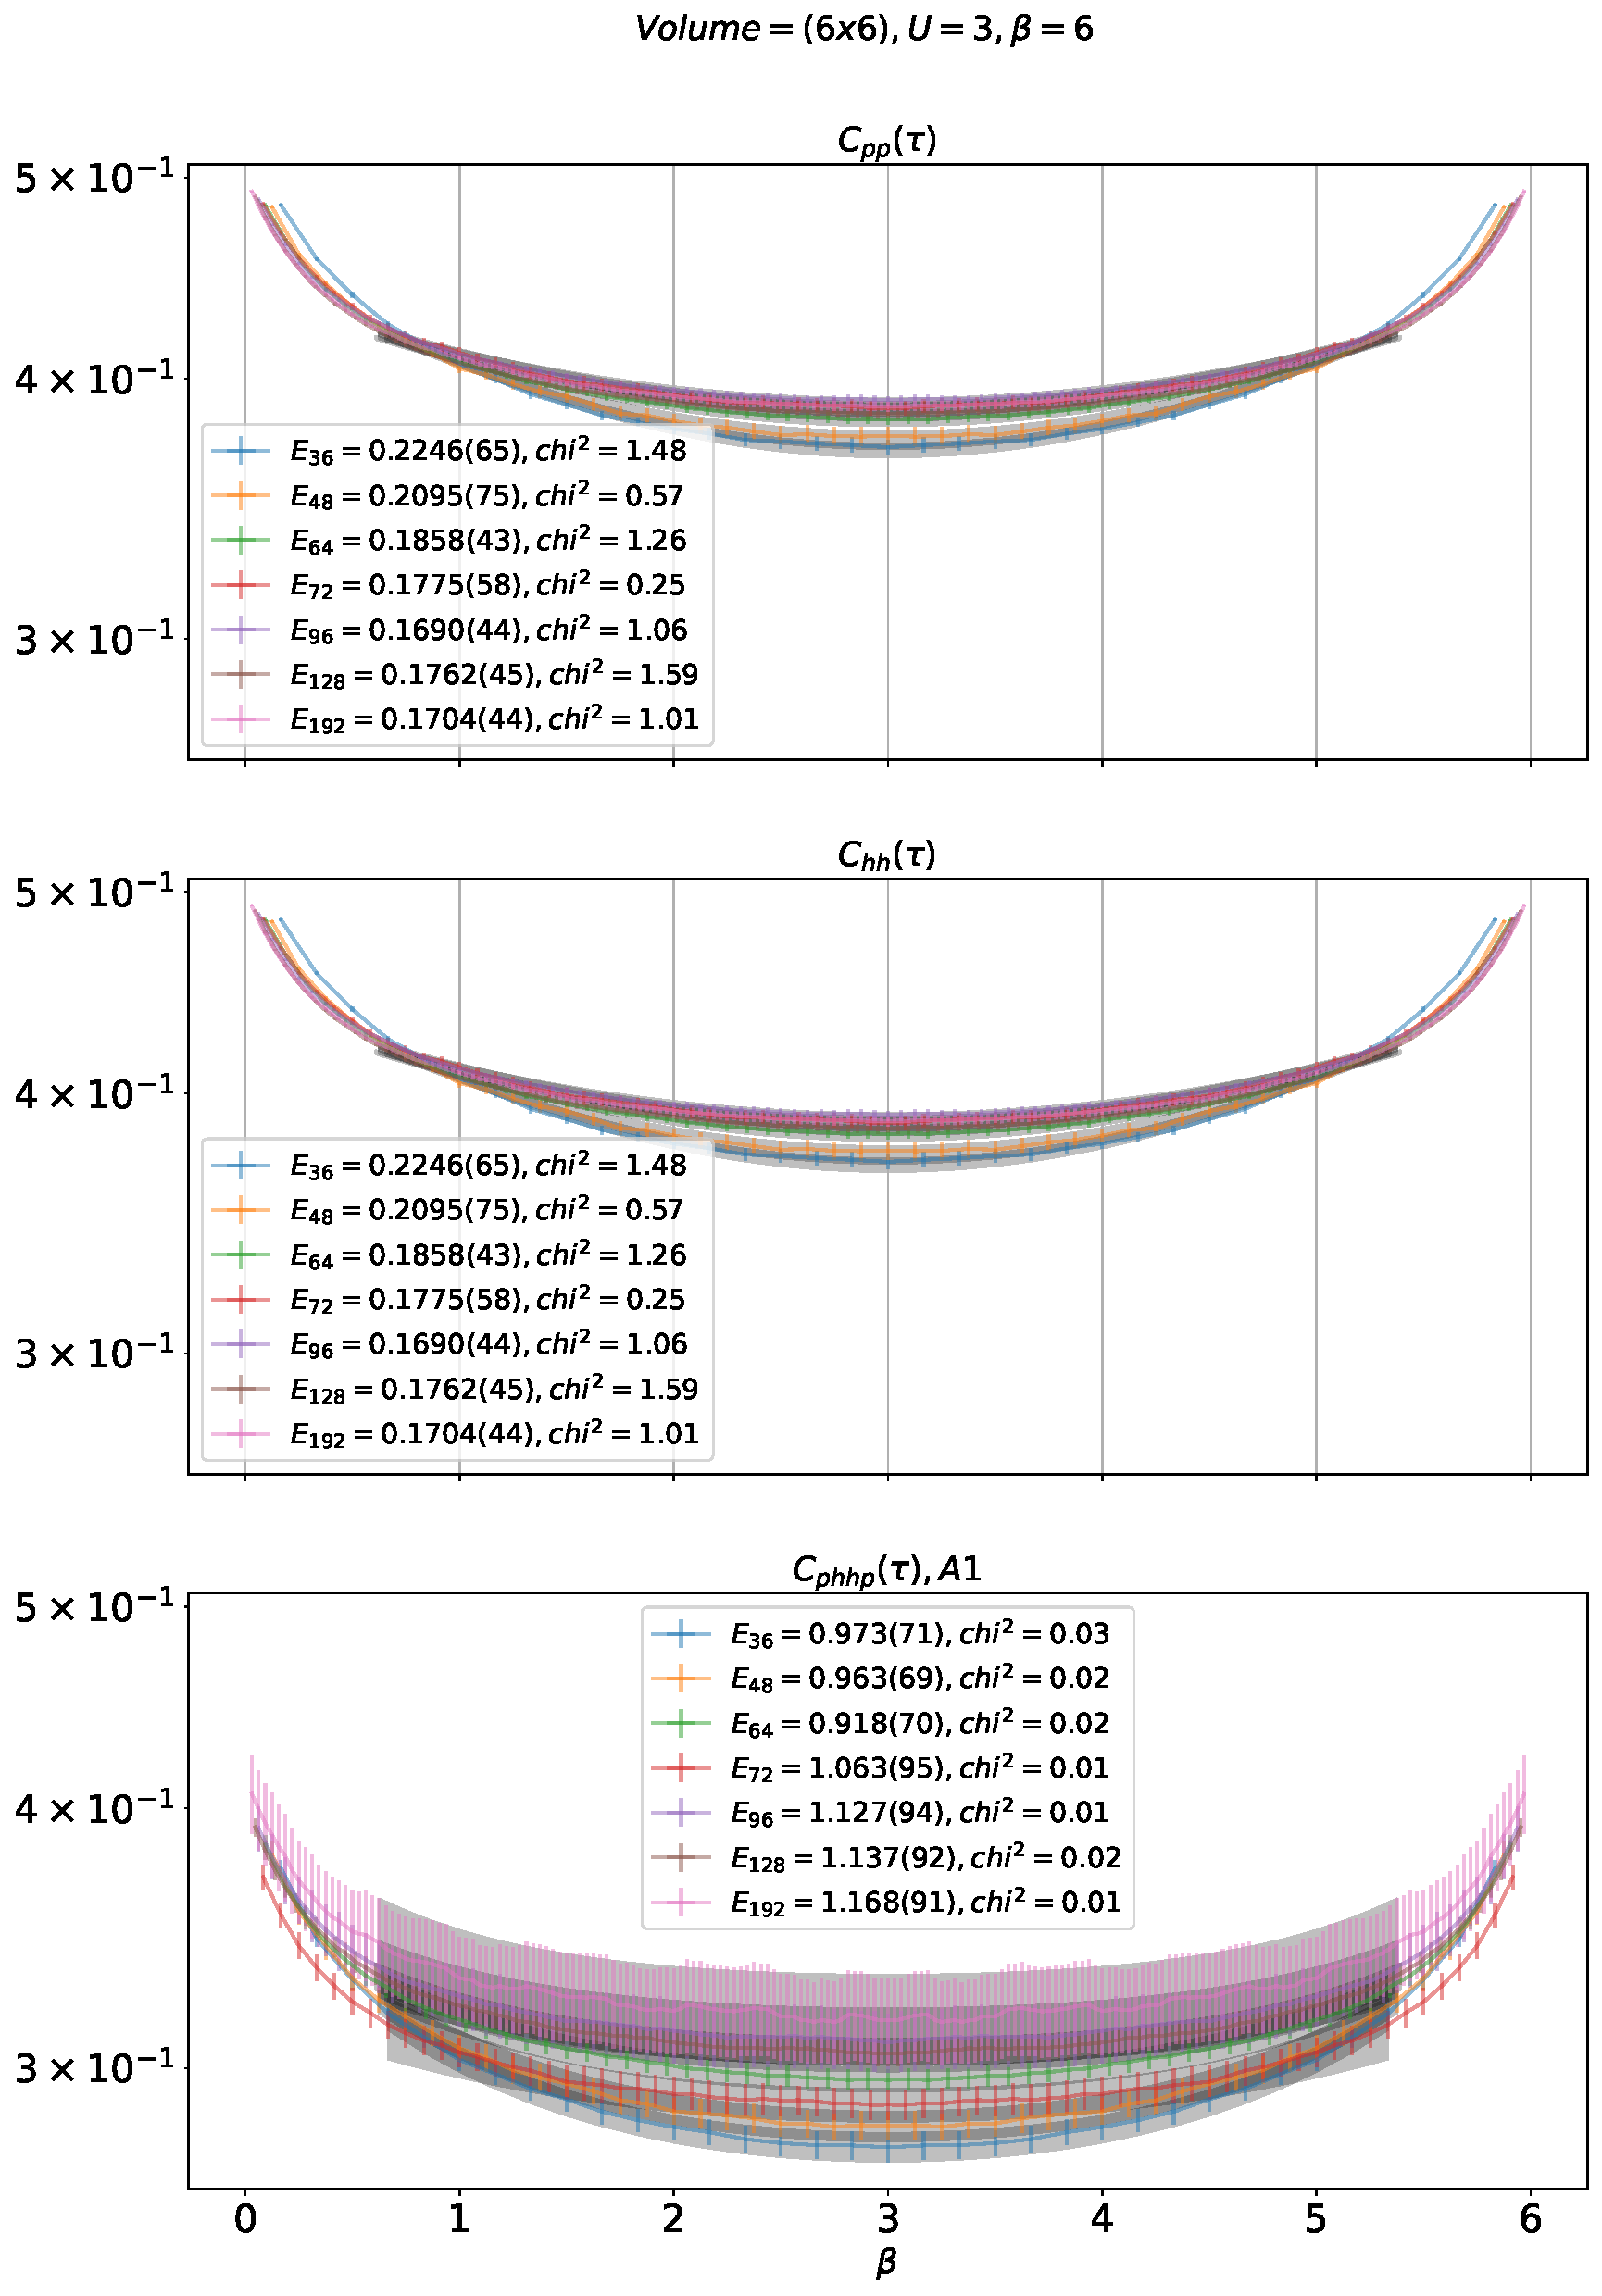
\includegraphics[width=\linewidth]{phhp-0-A1_6x6_U3.0_B6.0.pdf}
  \end{subfigure}%
  \begin{subfigure}{.5\textwidth}
    \centering
    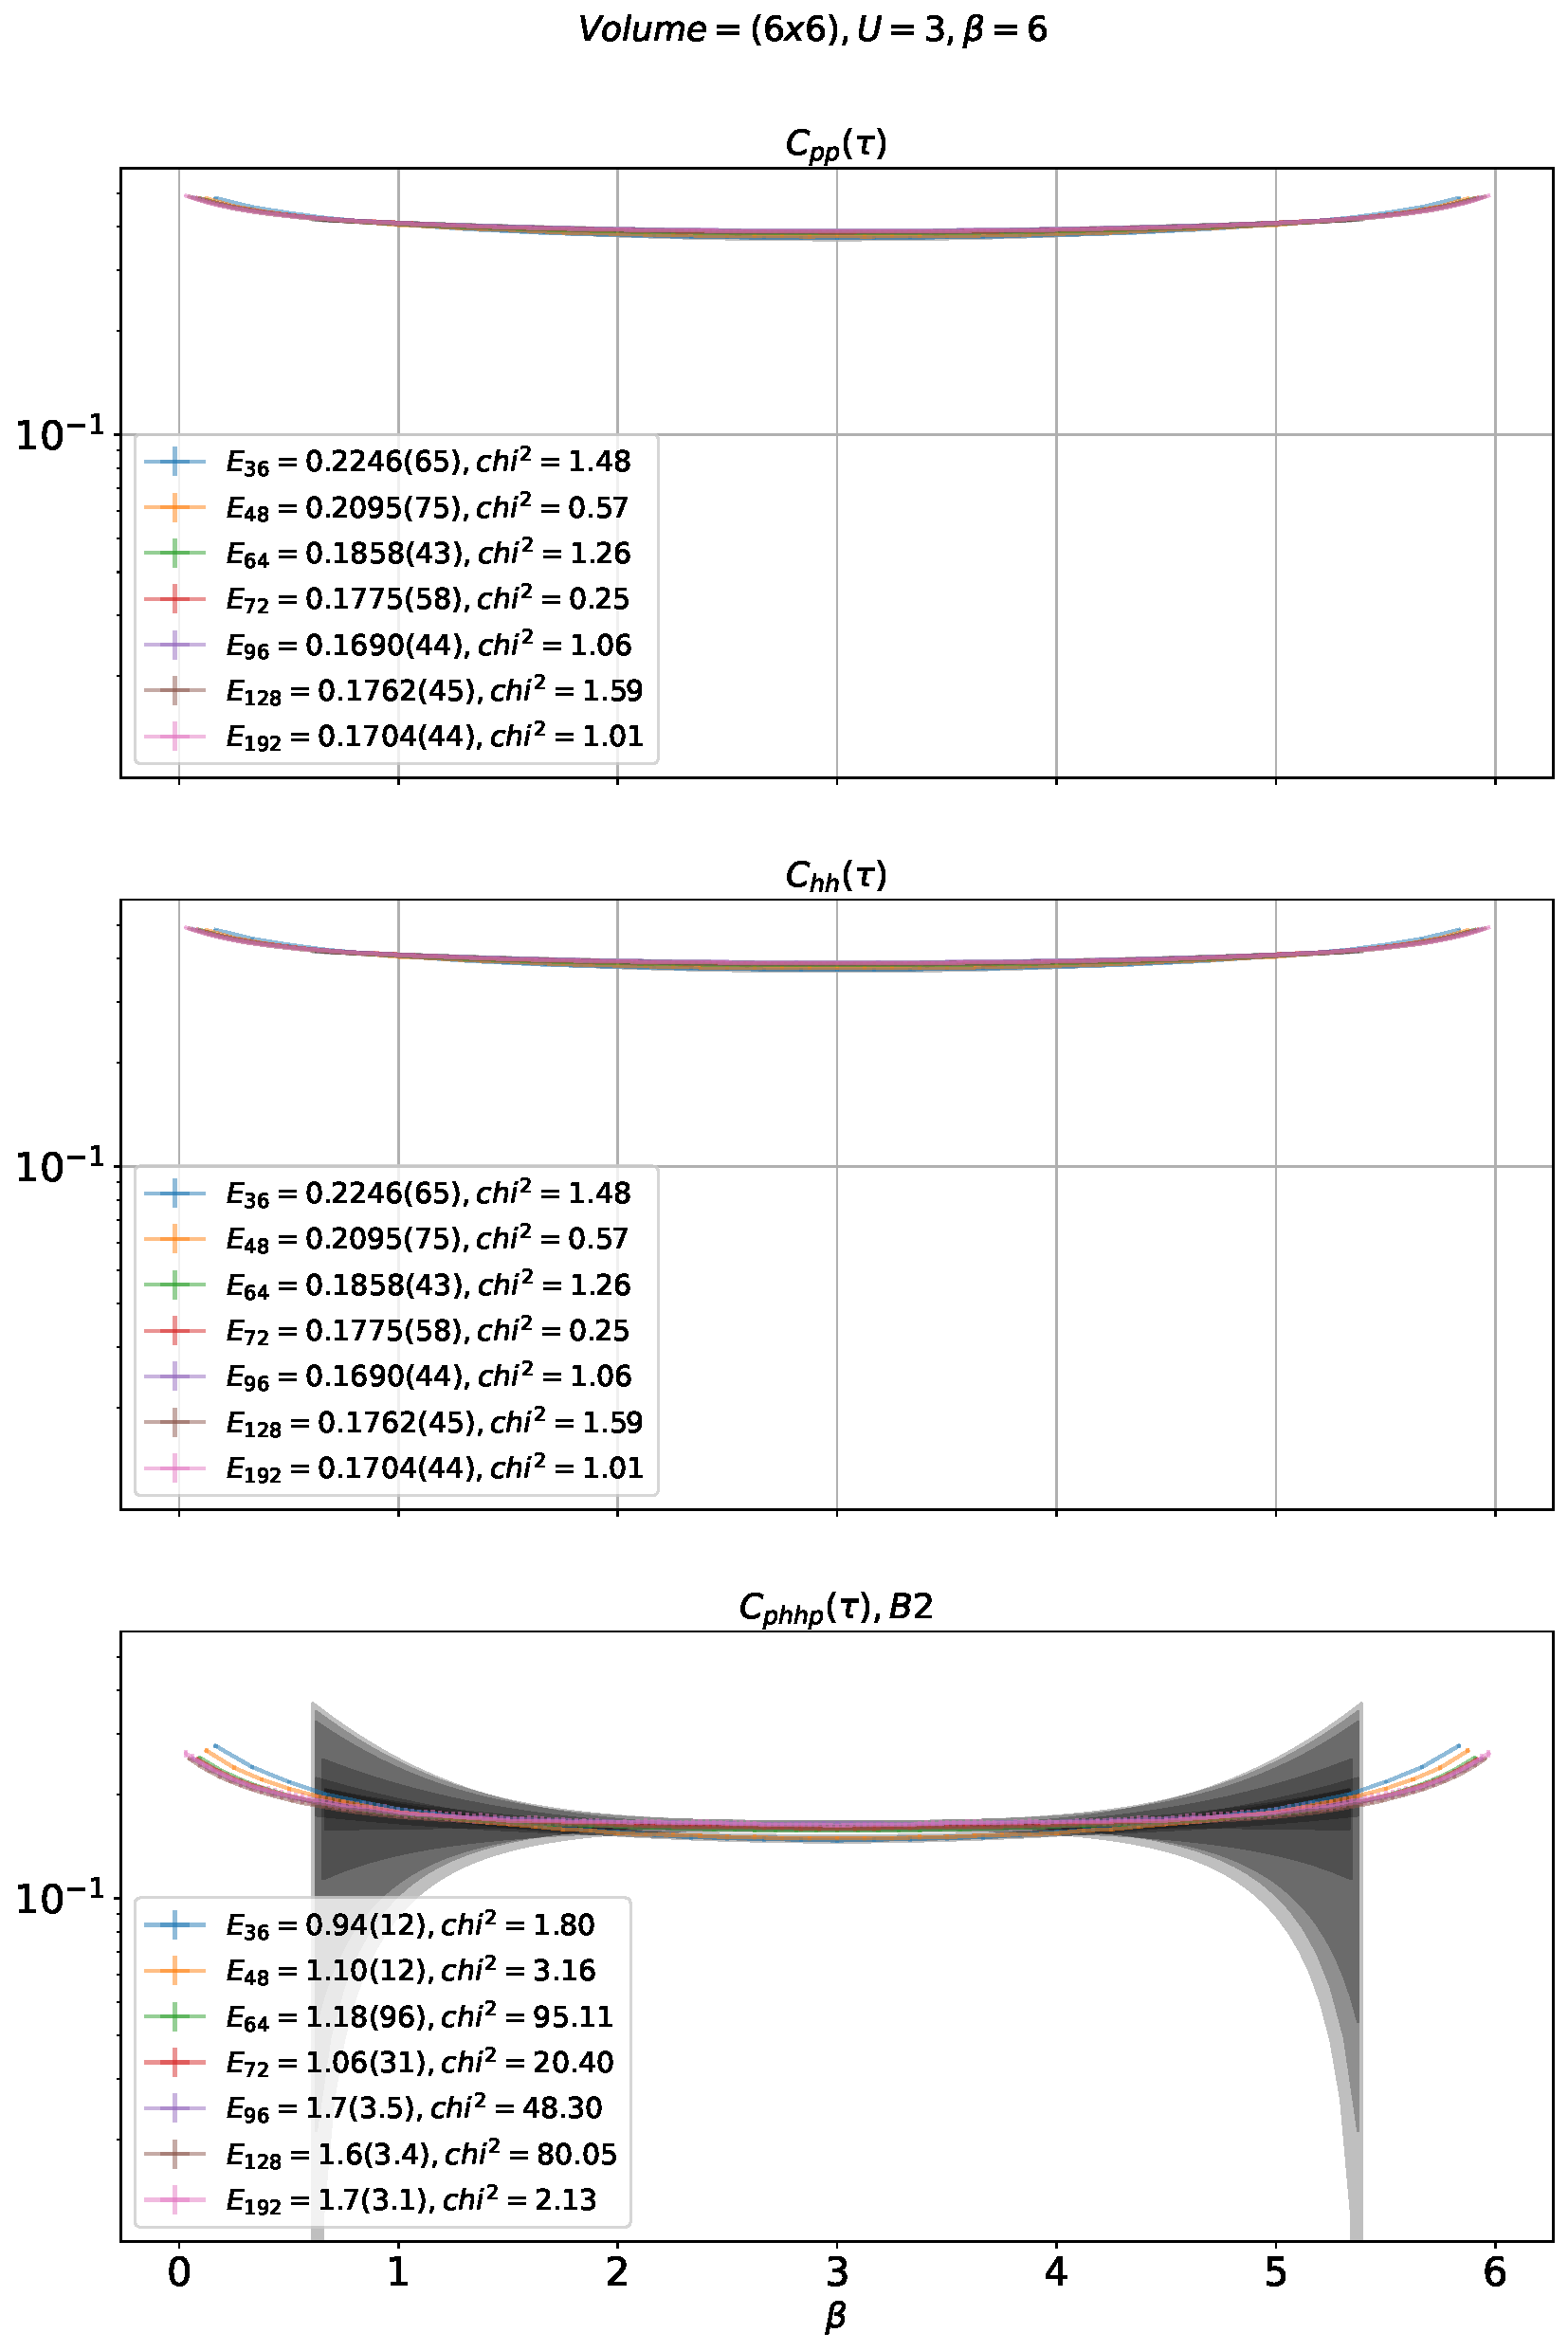
\includegraphics[width=\linewidth]{phhp-0-B2_6x6_U3.0_B6.0.pdf}
  \end{subfigure}
  \begin{subfigure}{.5\textwidth}
      \centering
      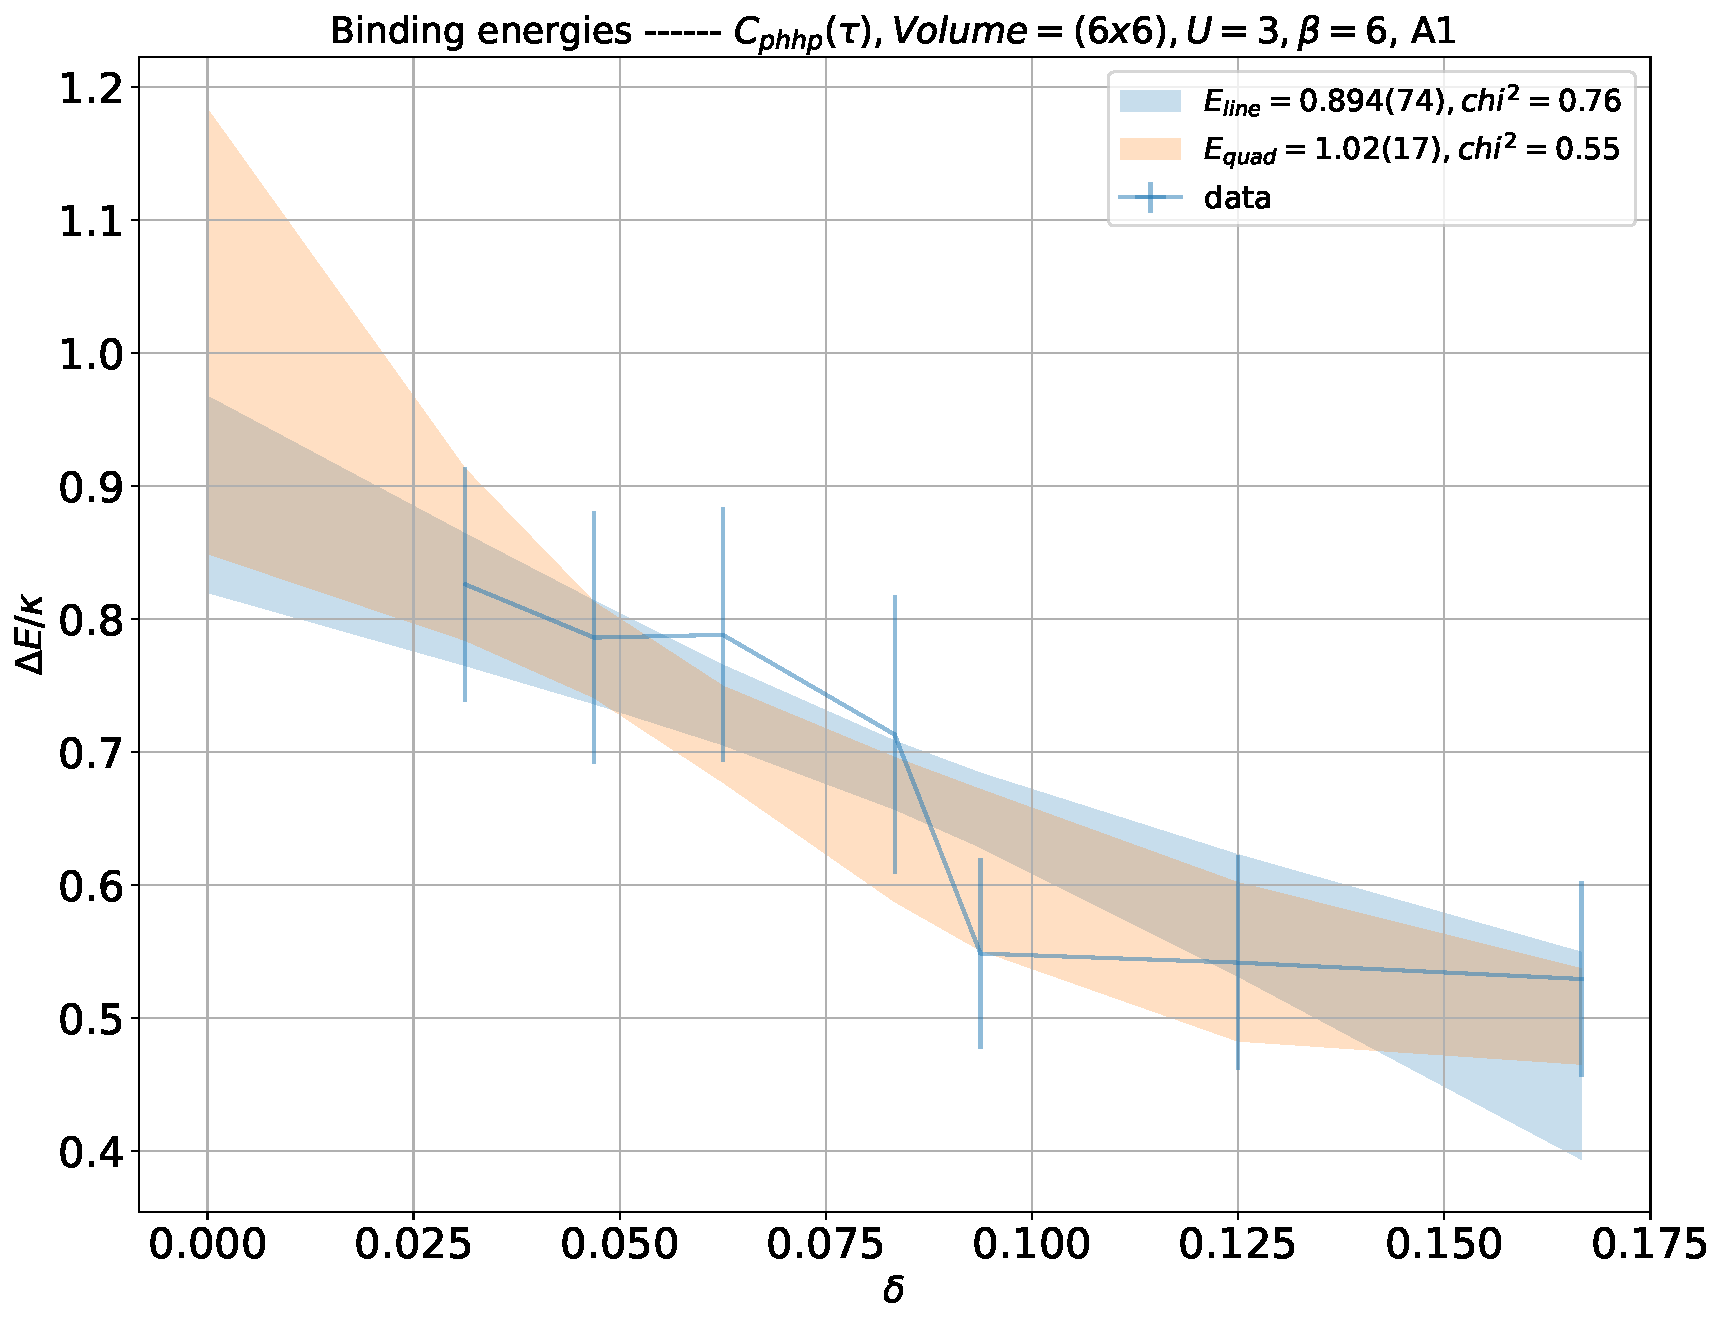
\includegraphics[width=\linewidth]{phhp-0-A1_6x6_U3.0_B6.0_cont.pdf}
  \end{subfigure}
  \begin{subfigure}{.5\textwidth}
      \centering
      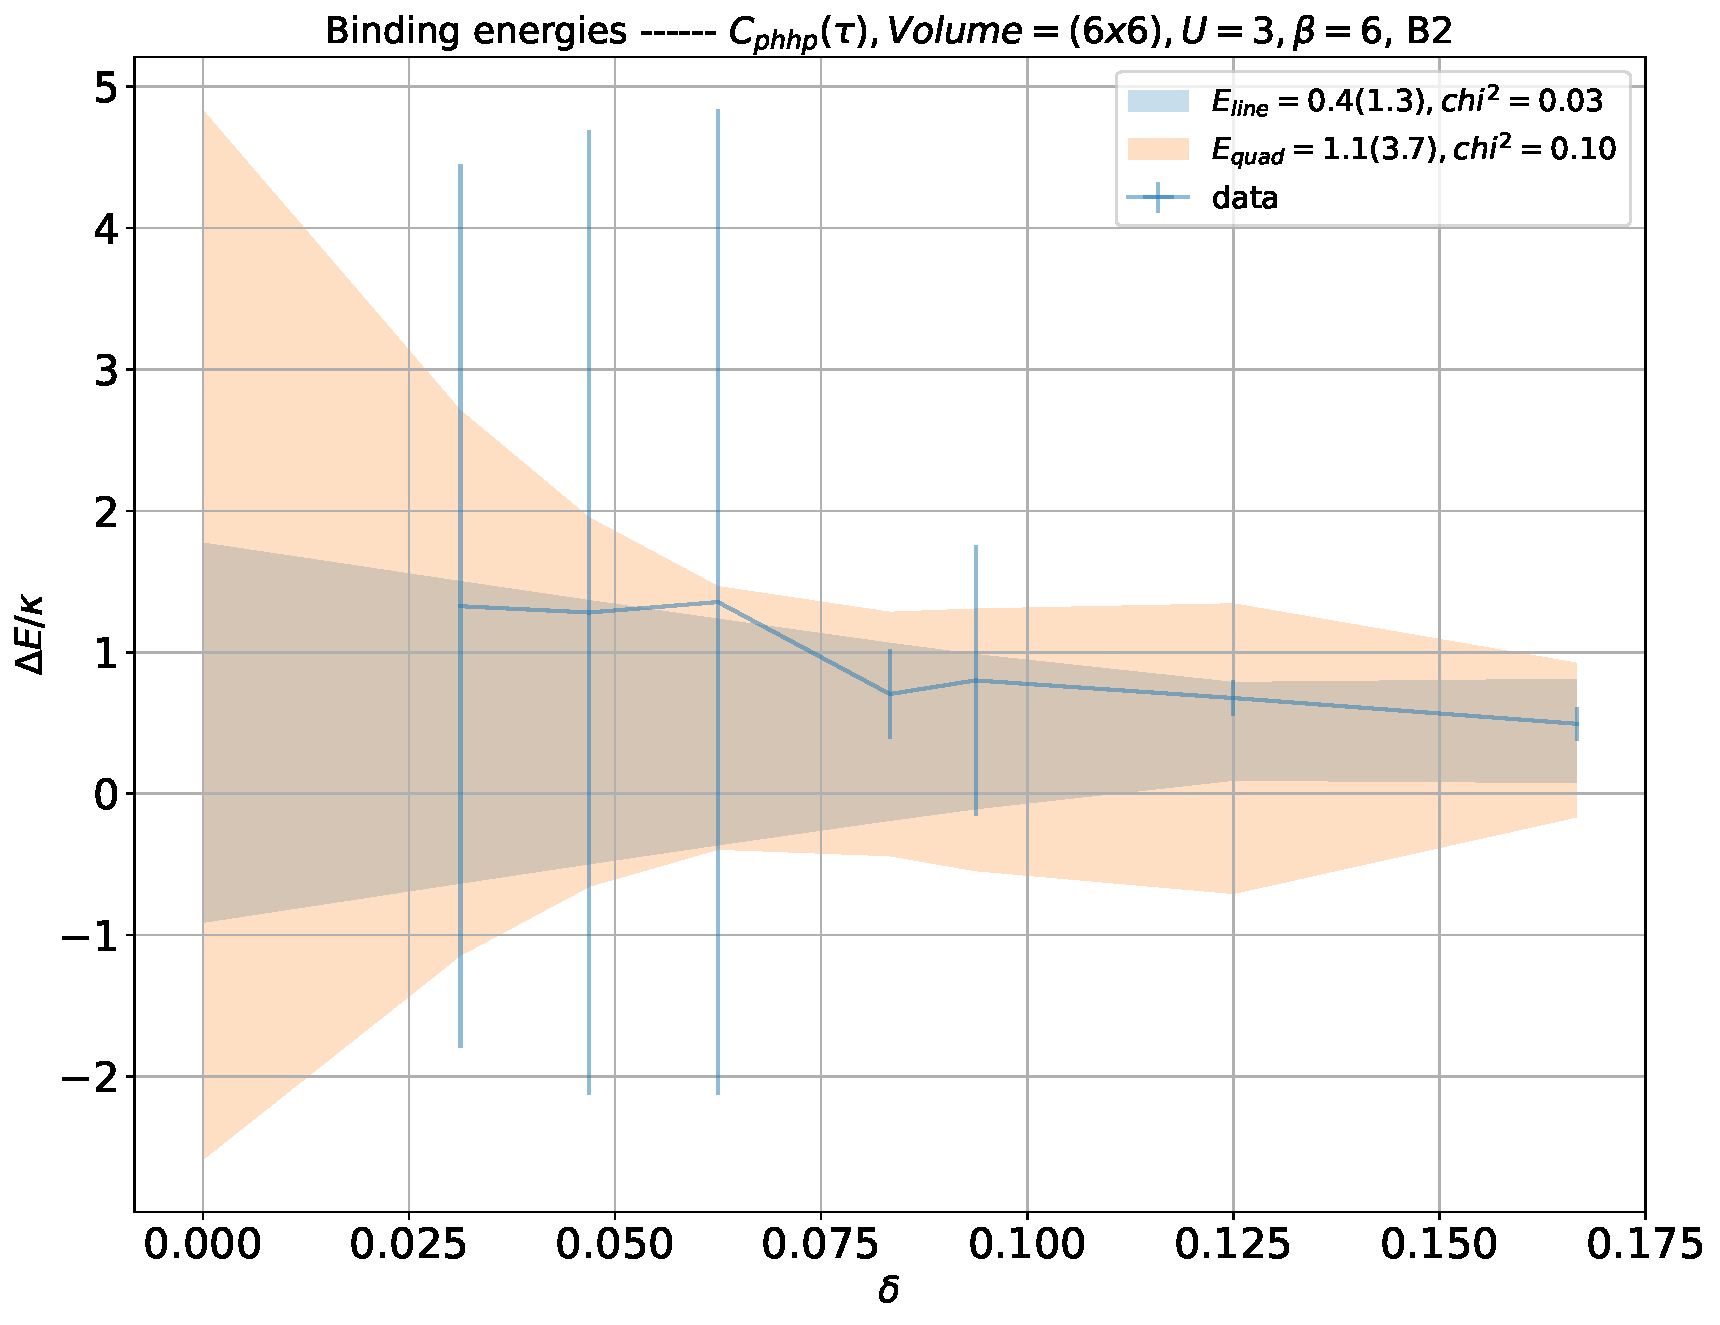
\includegraphics[width=\linewidth]{phhp-0-B2_6x6_U3.0_B6.0_cont.pdf}
  \end{subfigure}
  \caption{Binding energy extraction of the particle-hole pair at both irreducible representations, where we fit one- and two-body correlators for every $N_t$. This is followed by fitting a linear and a quadratic functions to the $\Delta E_{N_t}$ in order to extrapolate to the continuum limit ($N_t\to\infty$).}
  \label{fig:fig1}
\end{figure}

\begin{figure}
  \begin{subfigure}{.5\textwidth}
    \centering
    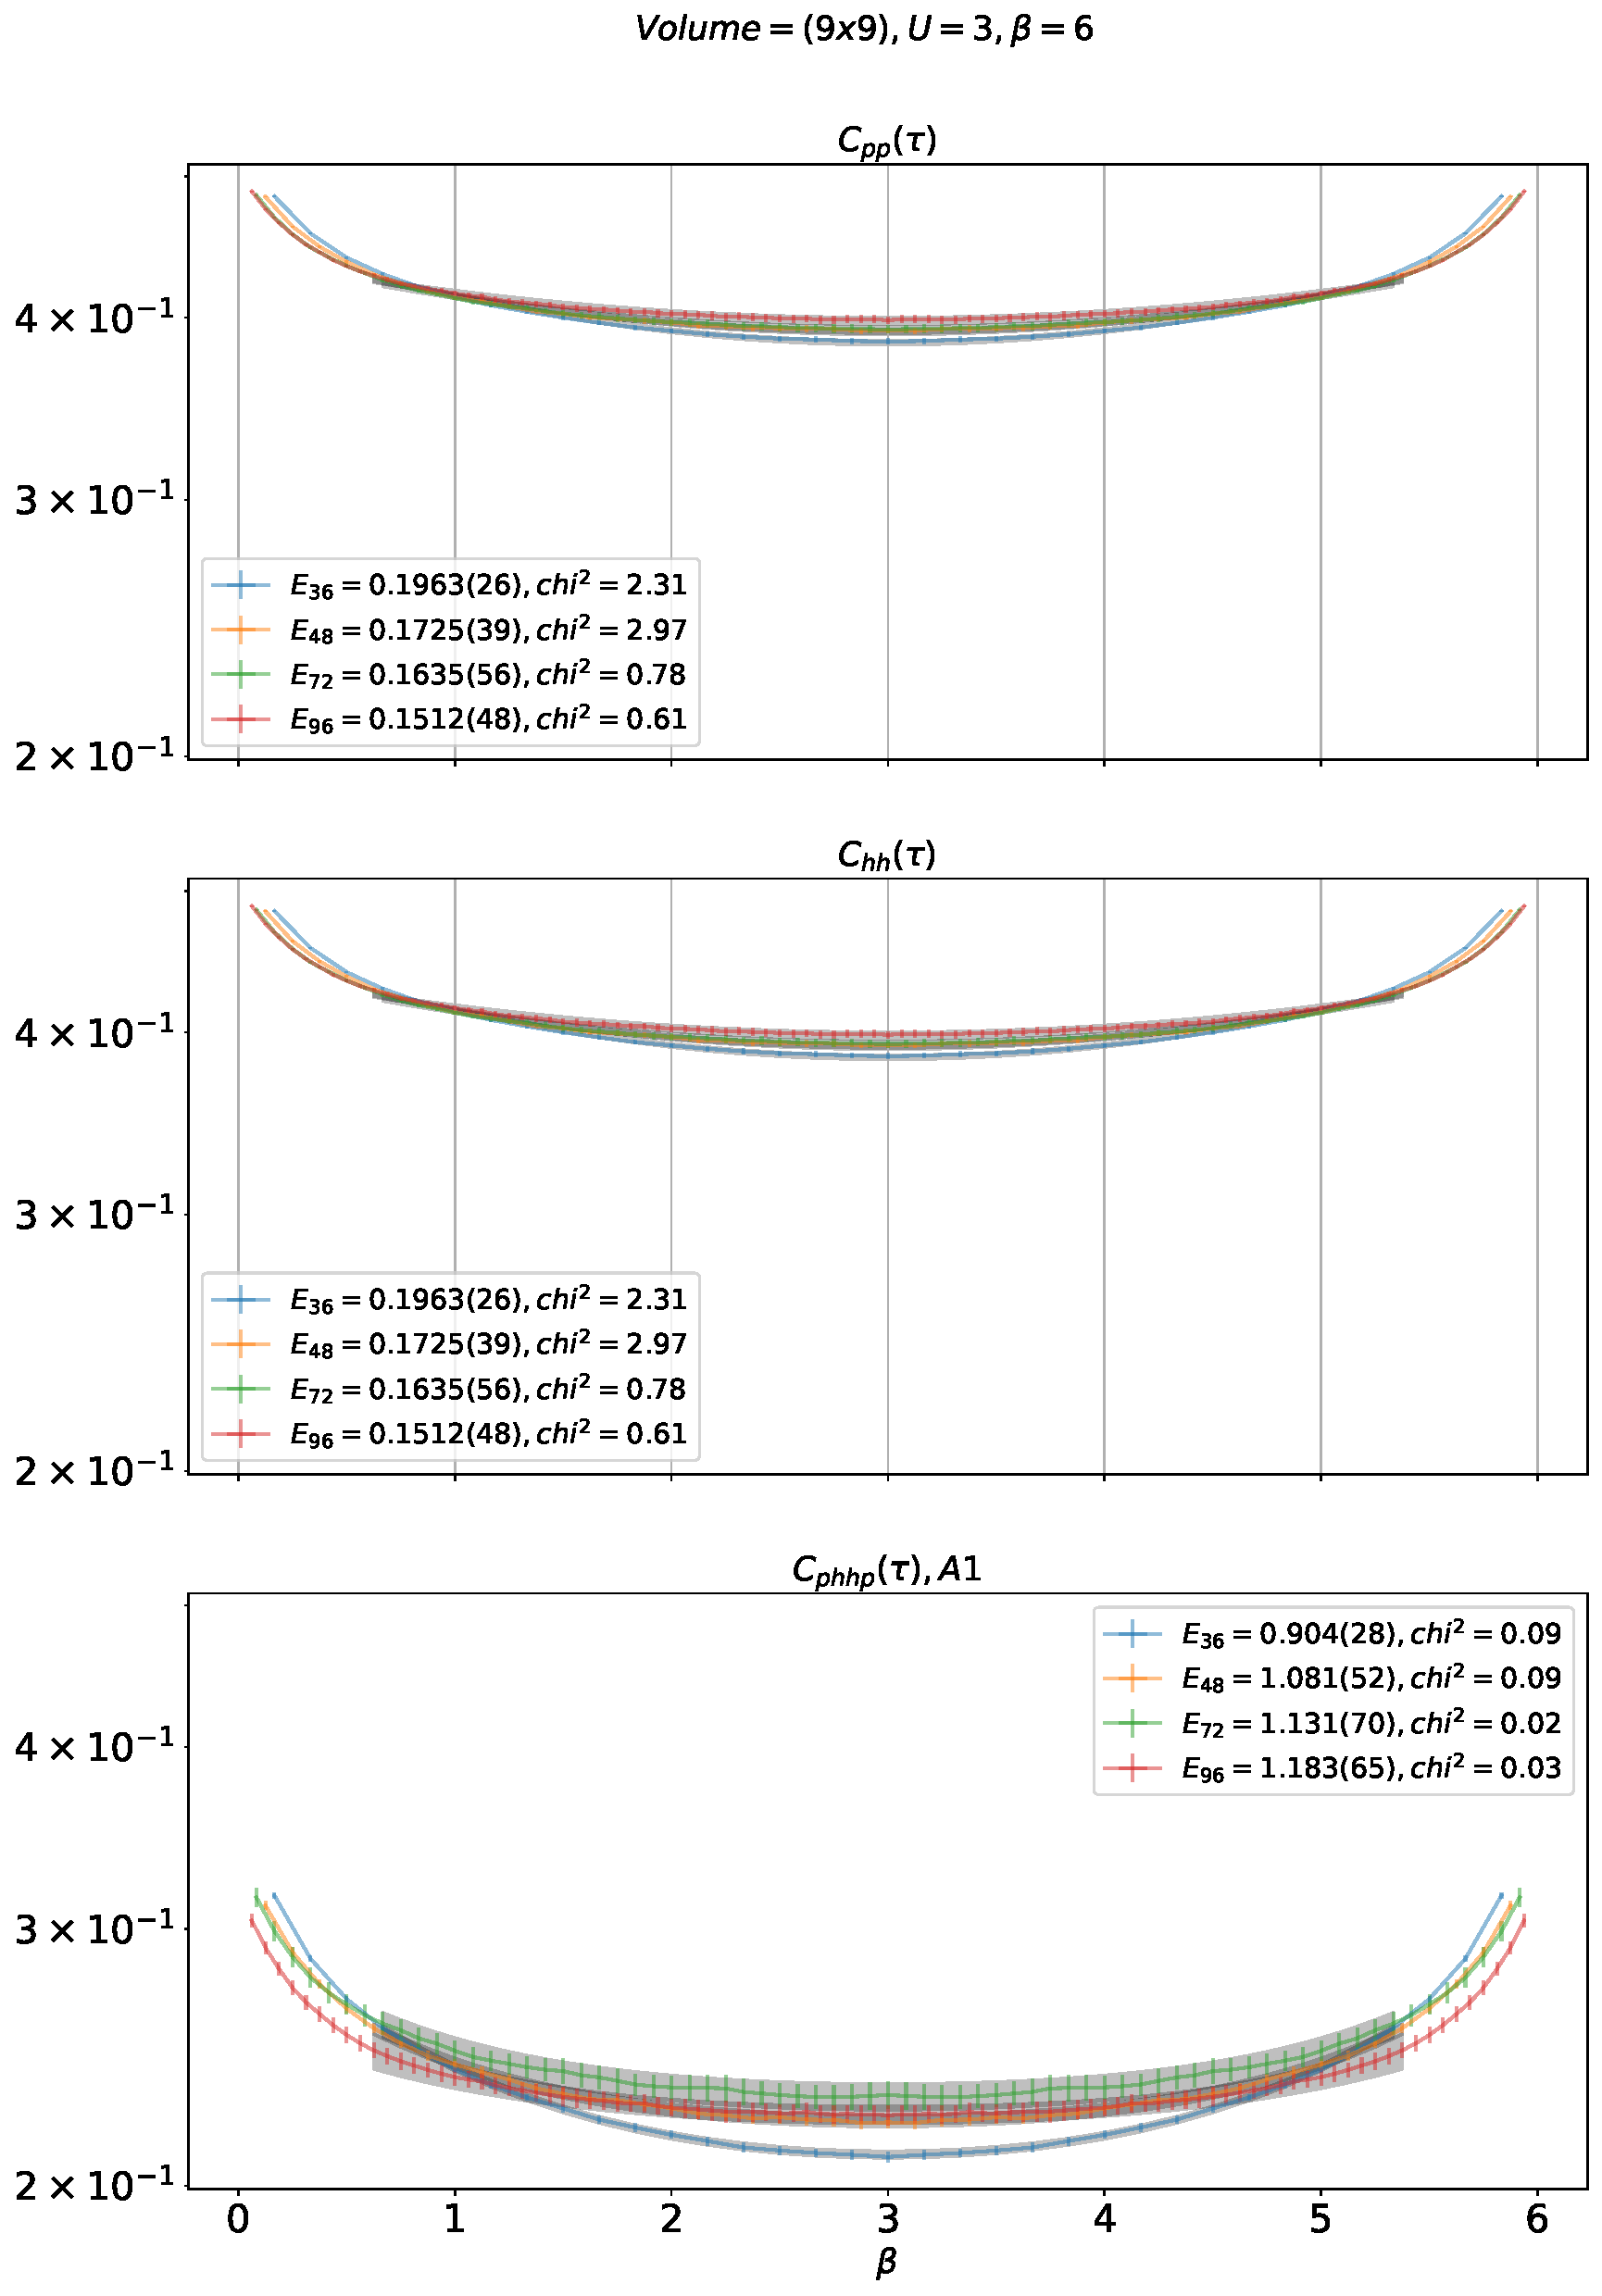
\includegraphics[width=\linewidth]{phhp-0-A1_9x9_U3_B6.pdf}
  \end{subfigure}%
  \begin{subfigure}{.5\textwidth}
    \centering
    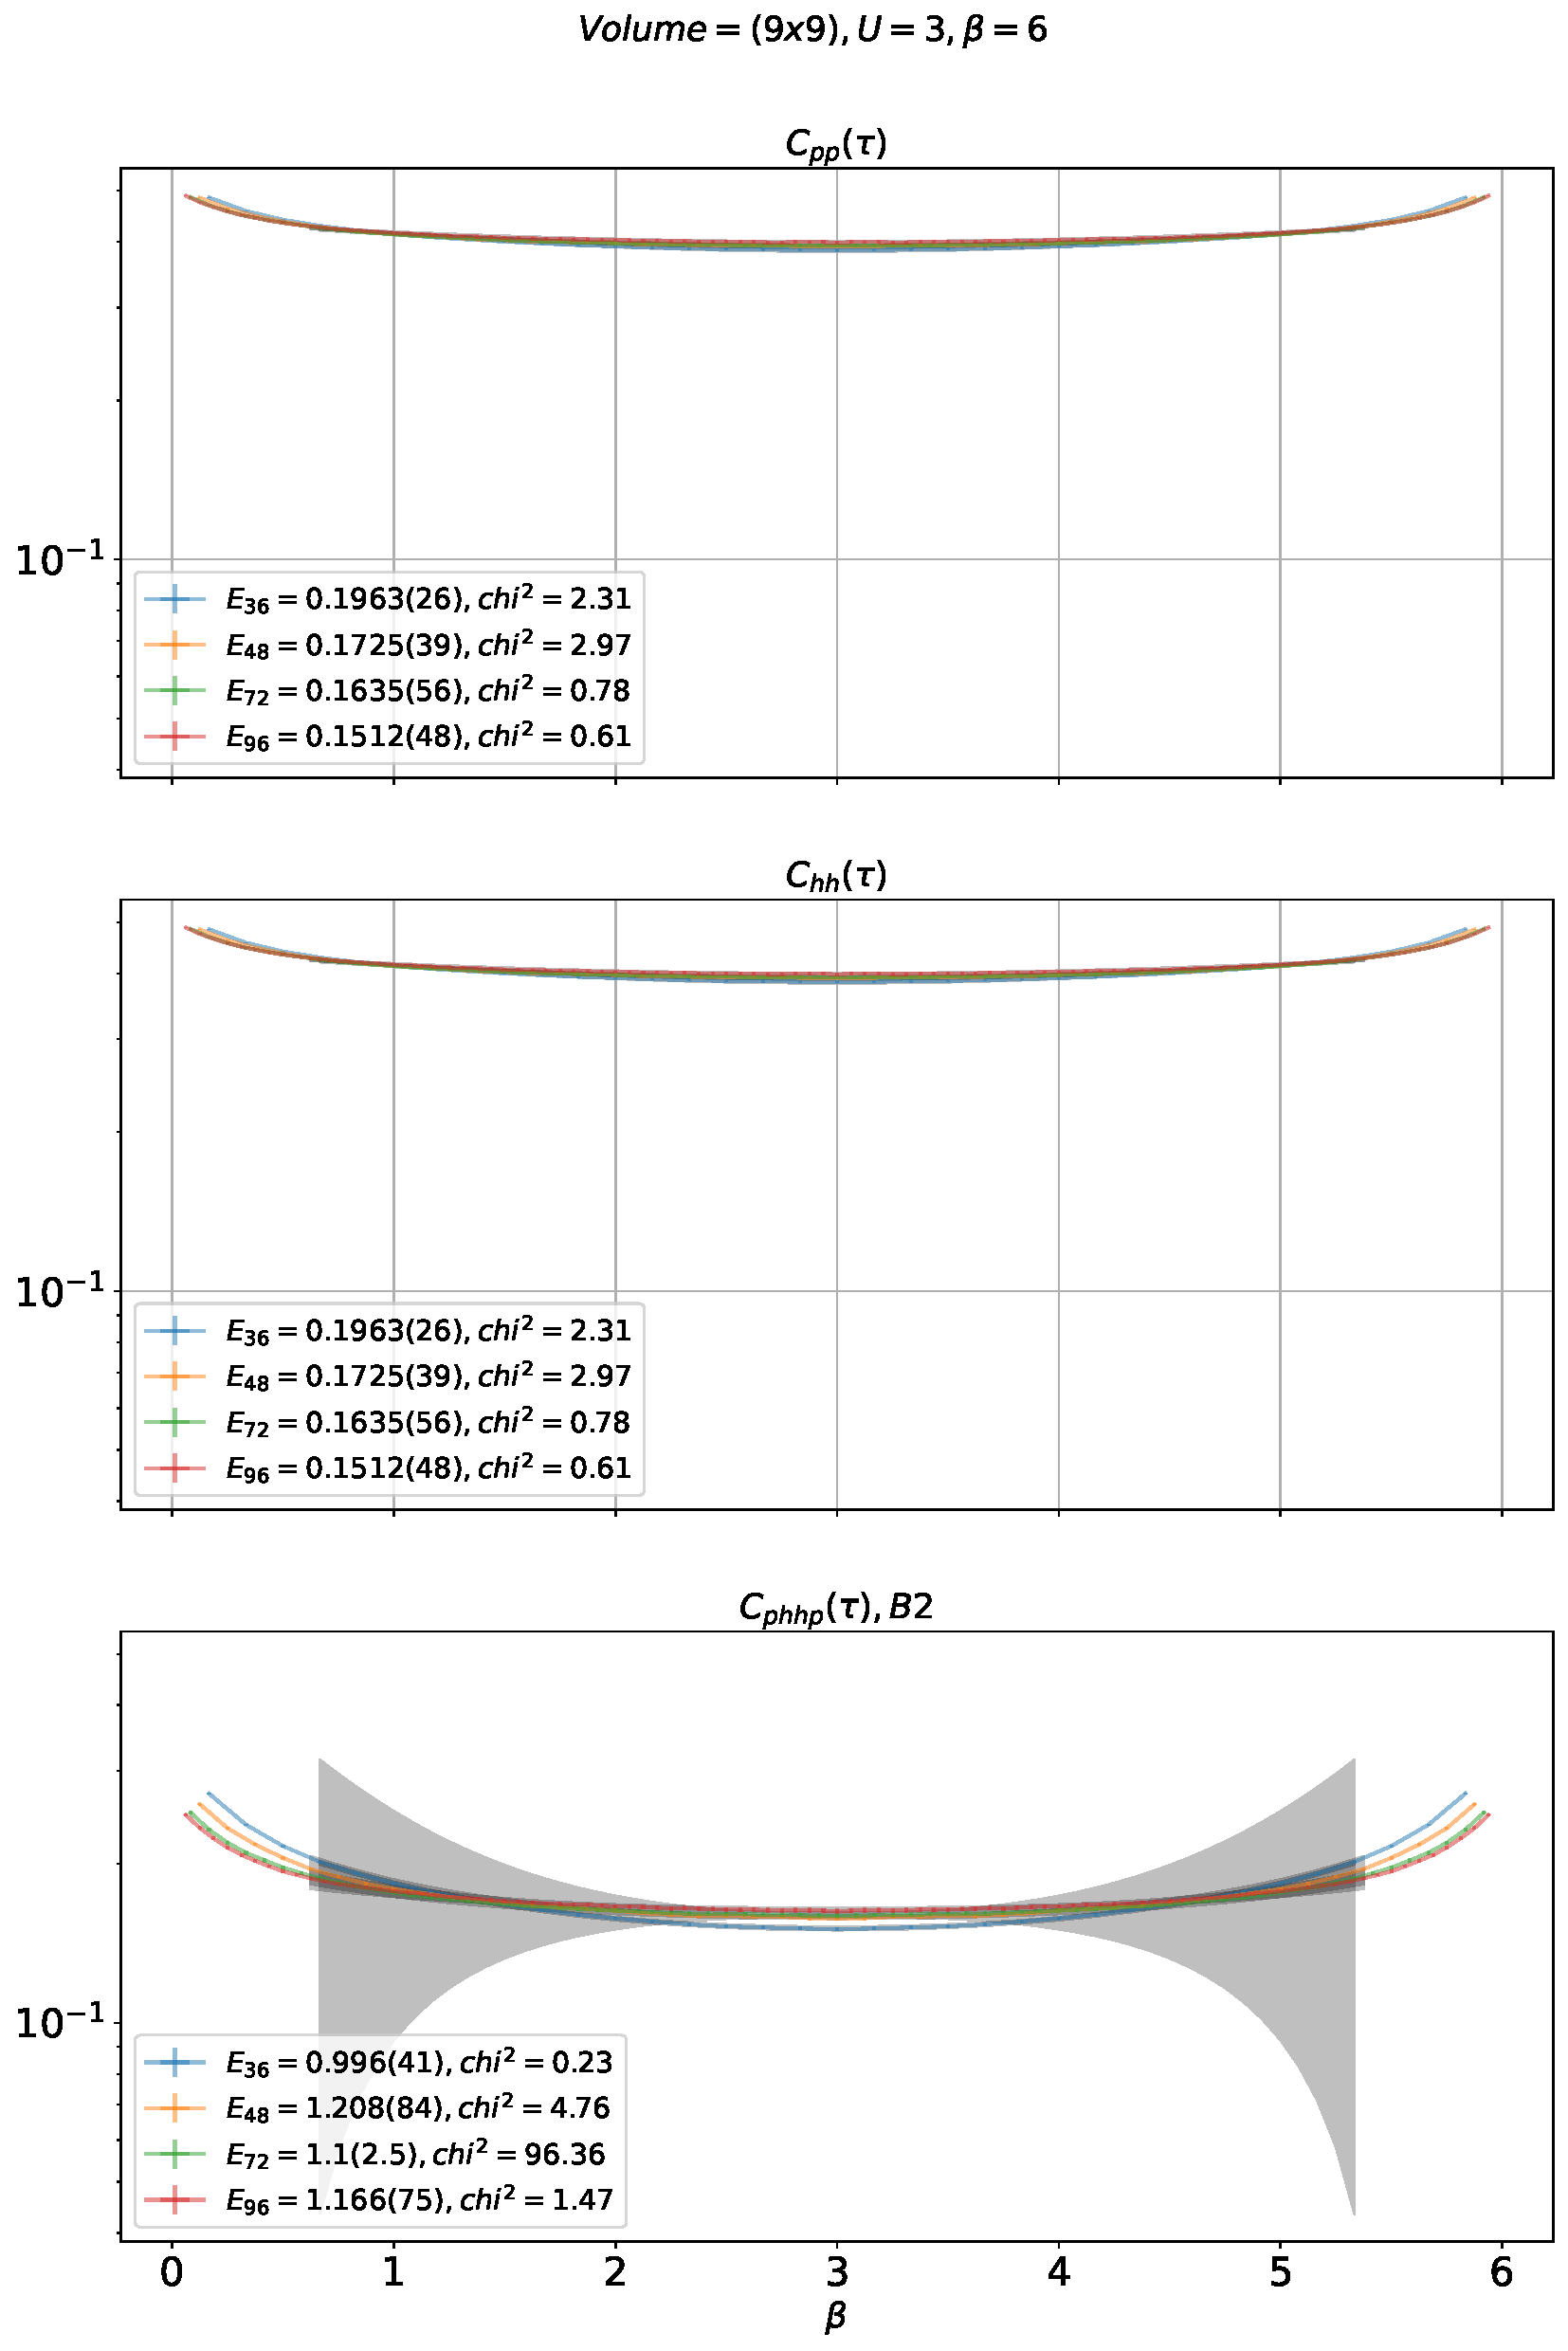
\includegraphics[width=\linewidth]{phhp-0-B2_9x9_U3_B6.pdf}
  \end{subfigure}
  \begin{subfigure}{.5\textwidth}
      \centering
      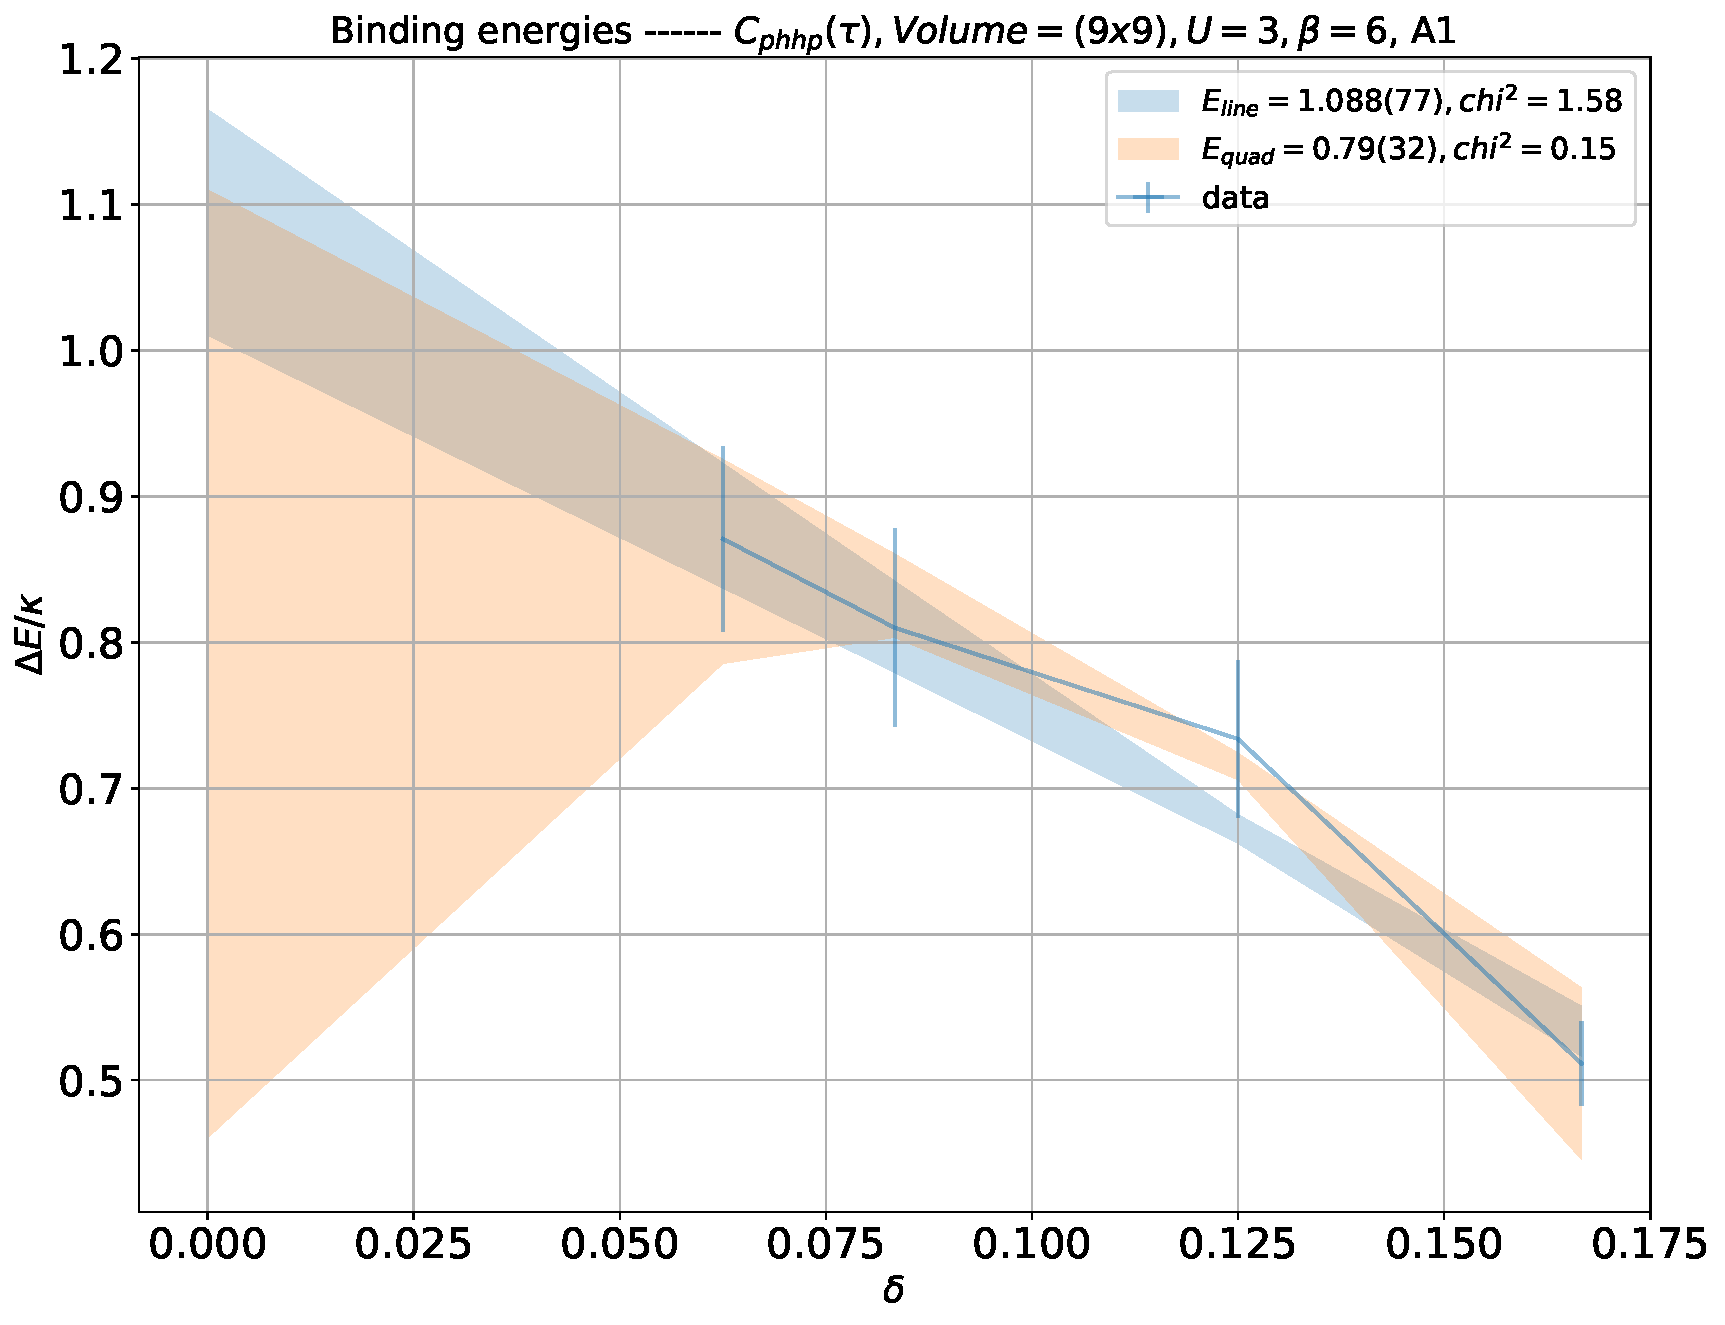
\includegraphics[width=\linewidth]{phhp-0-A1_9x9_U3_B6_cont.pdf}
  \end{subfigure}
  \begin{subfigure}{.5\textwidth}
      \centering
      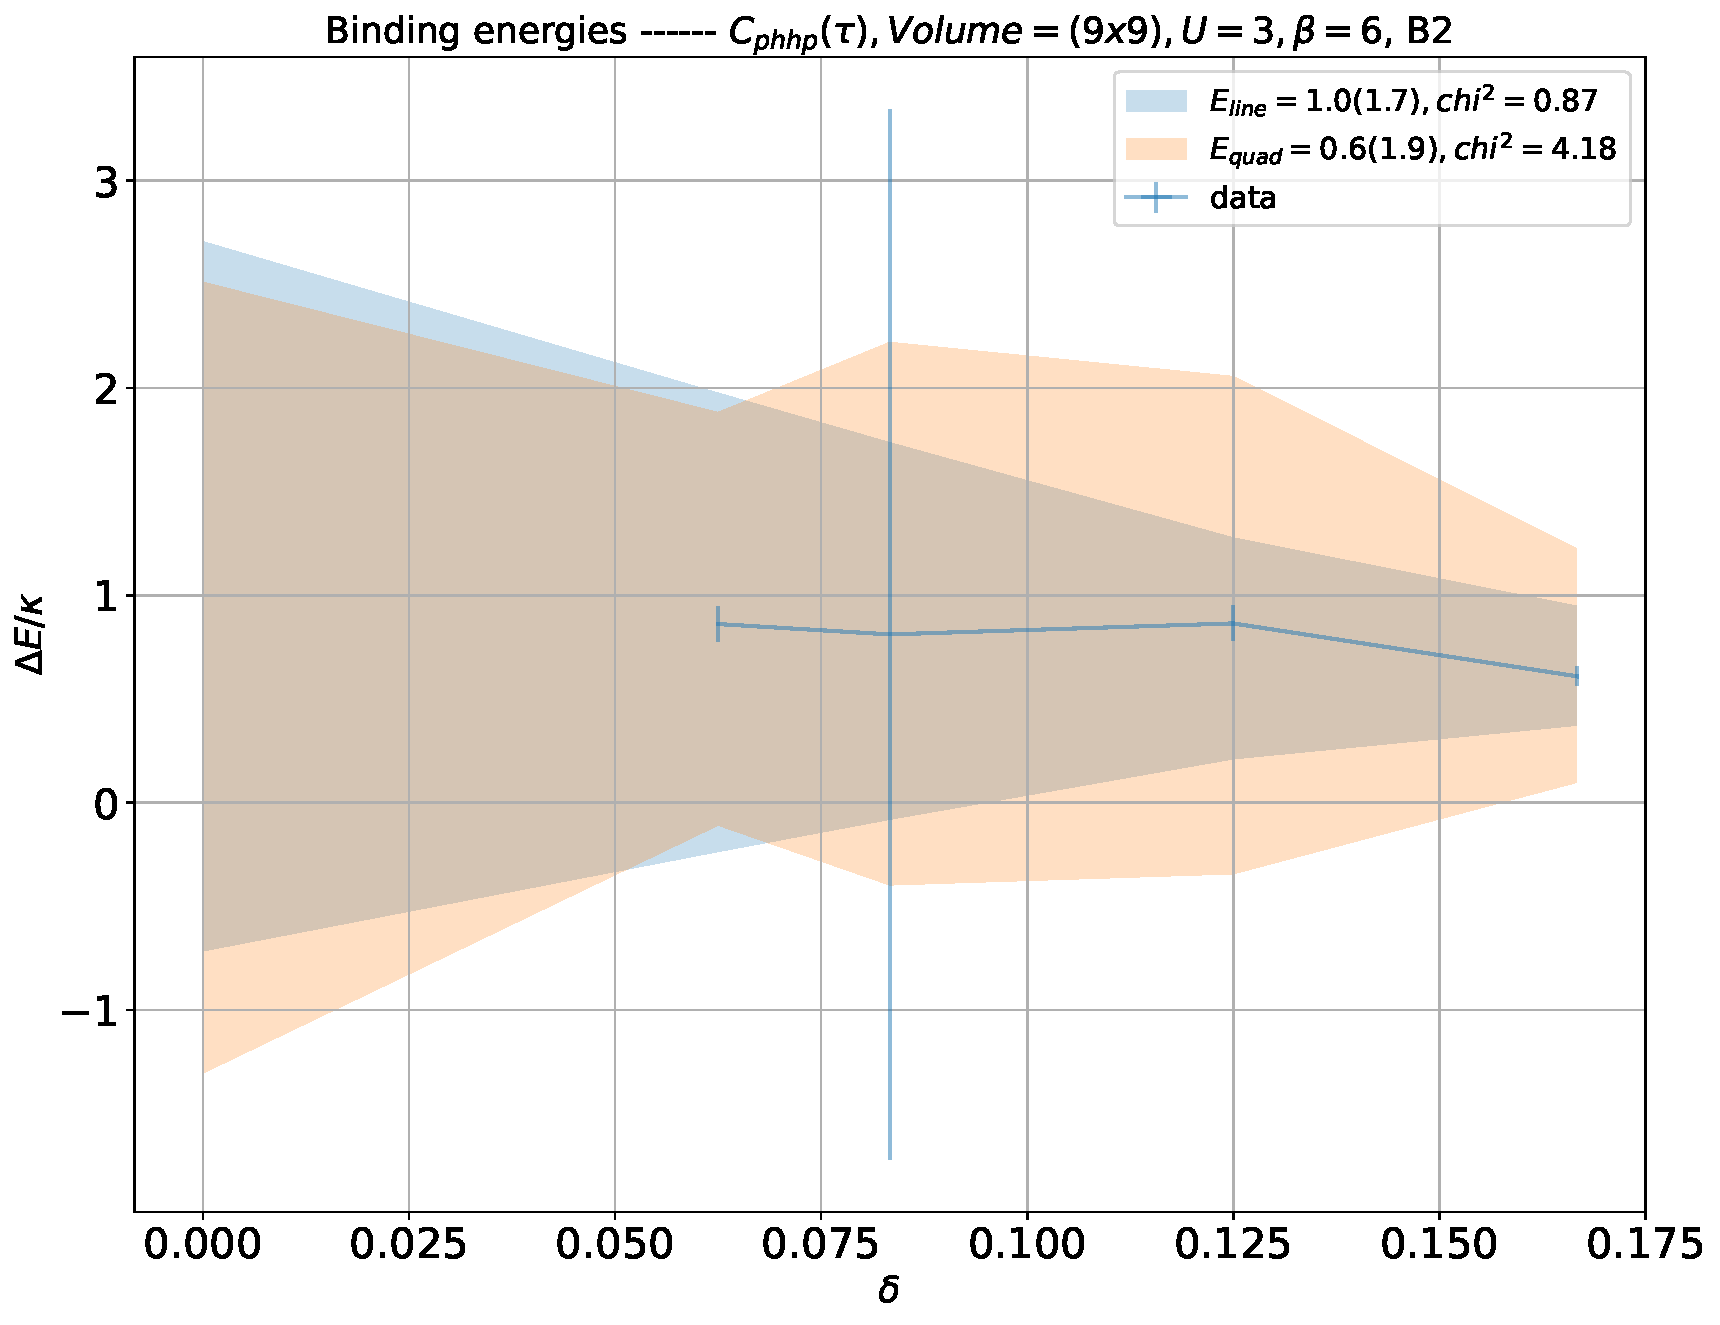
\includegraphics[width=\linewidth]{phhp-0-B2_9x9_U3_B6_cont.pdf}
  \end{subfigure}
  \caption{Binding energy extraction of the particle-hole pair at both irreducible representations, where we fit one- and two-body correlators for every $N_t$. This is followed by fitting a linear and a quadratic functions to the $\Delta E_{N_t}$ in order to extrapolate to the continuum limit ($N_t\to\infty$).}
  \label{fig:fig2}
\end{figure}

\begin{figure}
  \begin{subfigure}{.5\textwidth}
    \centering
    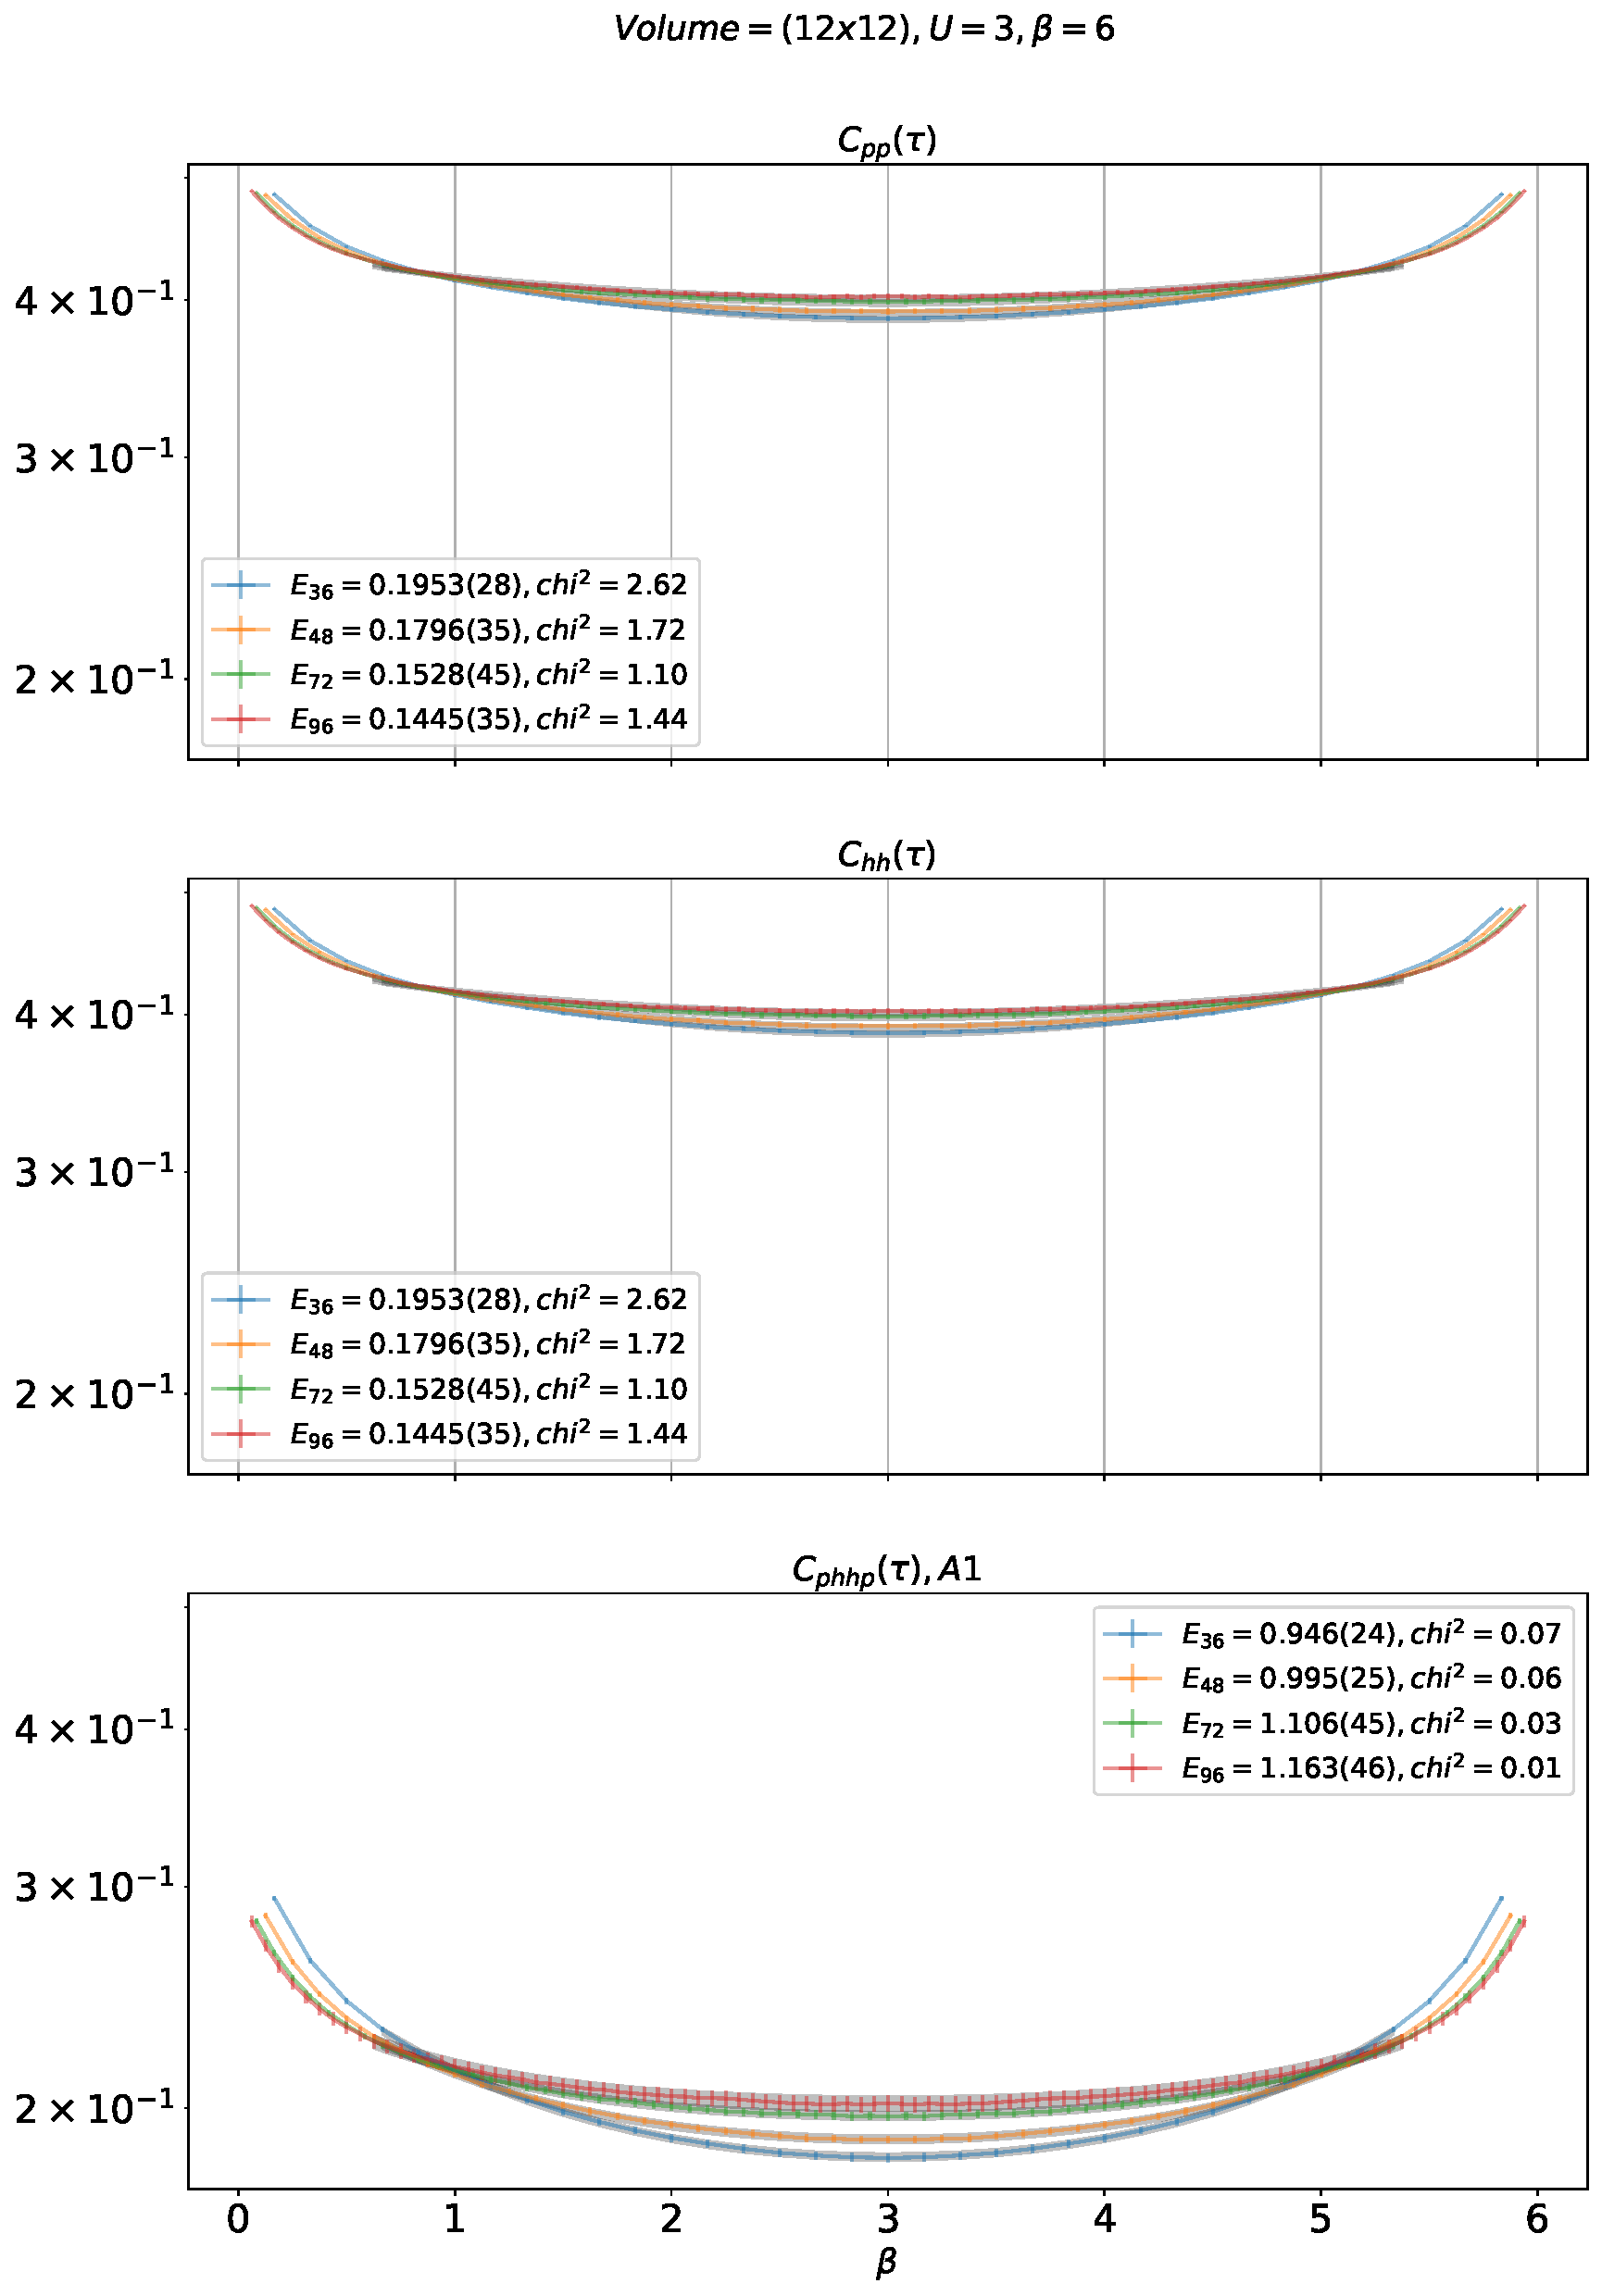
\includegraphics[width=\linewidth]{phhp-0-A1_12x12_U3_B6.pdf}
  \end{subfigure}%
  \begin{subfigure}{.5\textwidth}
    \centering
    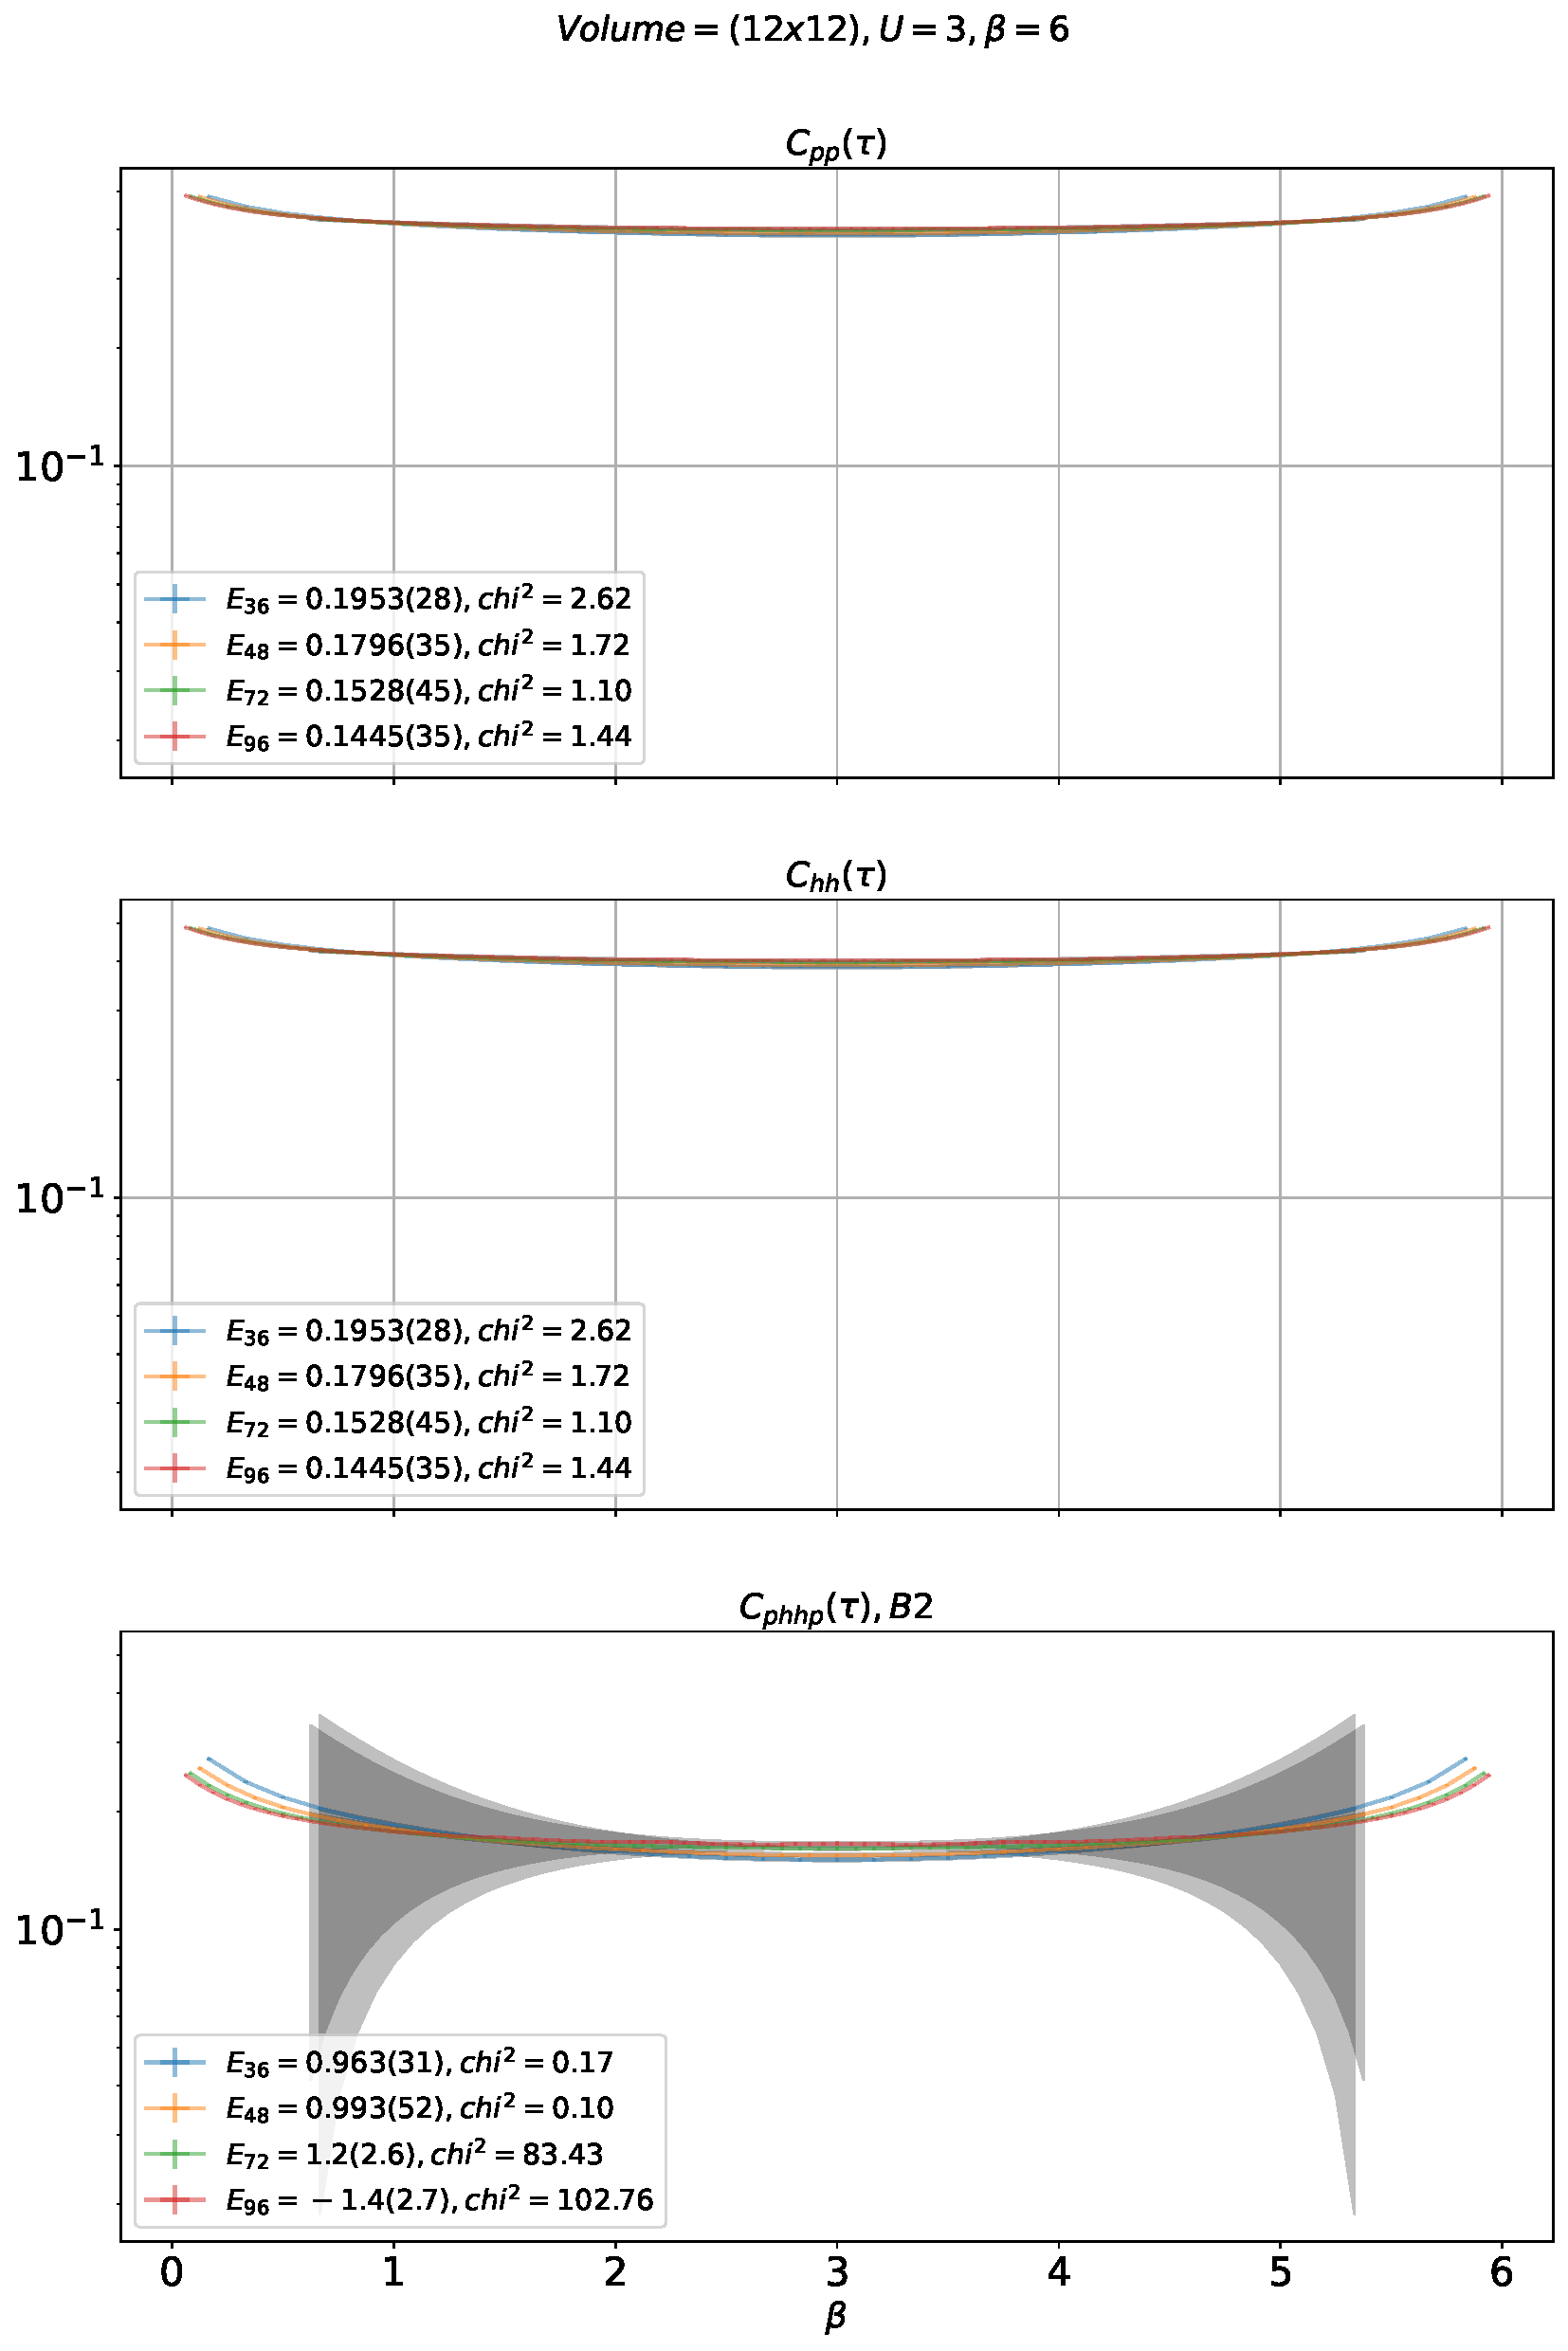
\includegraphics[width=\linewidth]{phhp-0-B2_12x12_U3_B6.pdf}
  \end{subfigure}
  \begin{subfigure}{.5\textwidth}
      \centering
      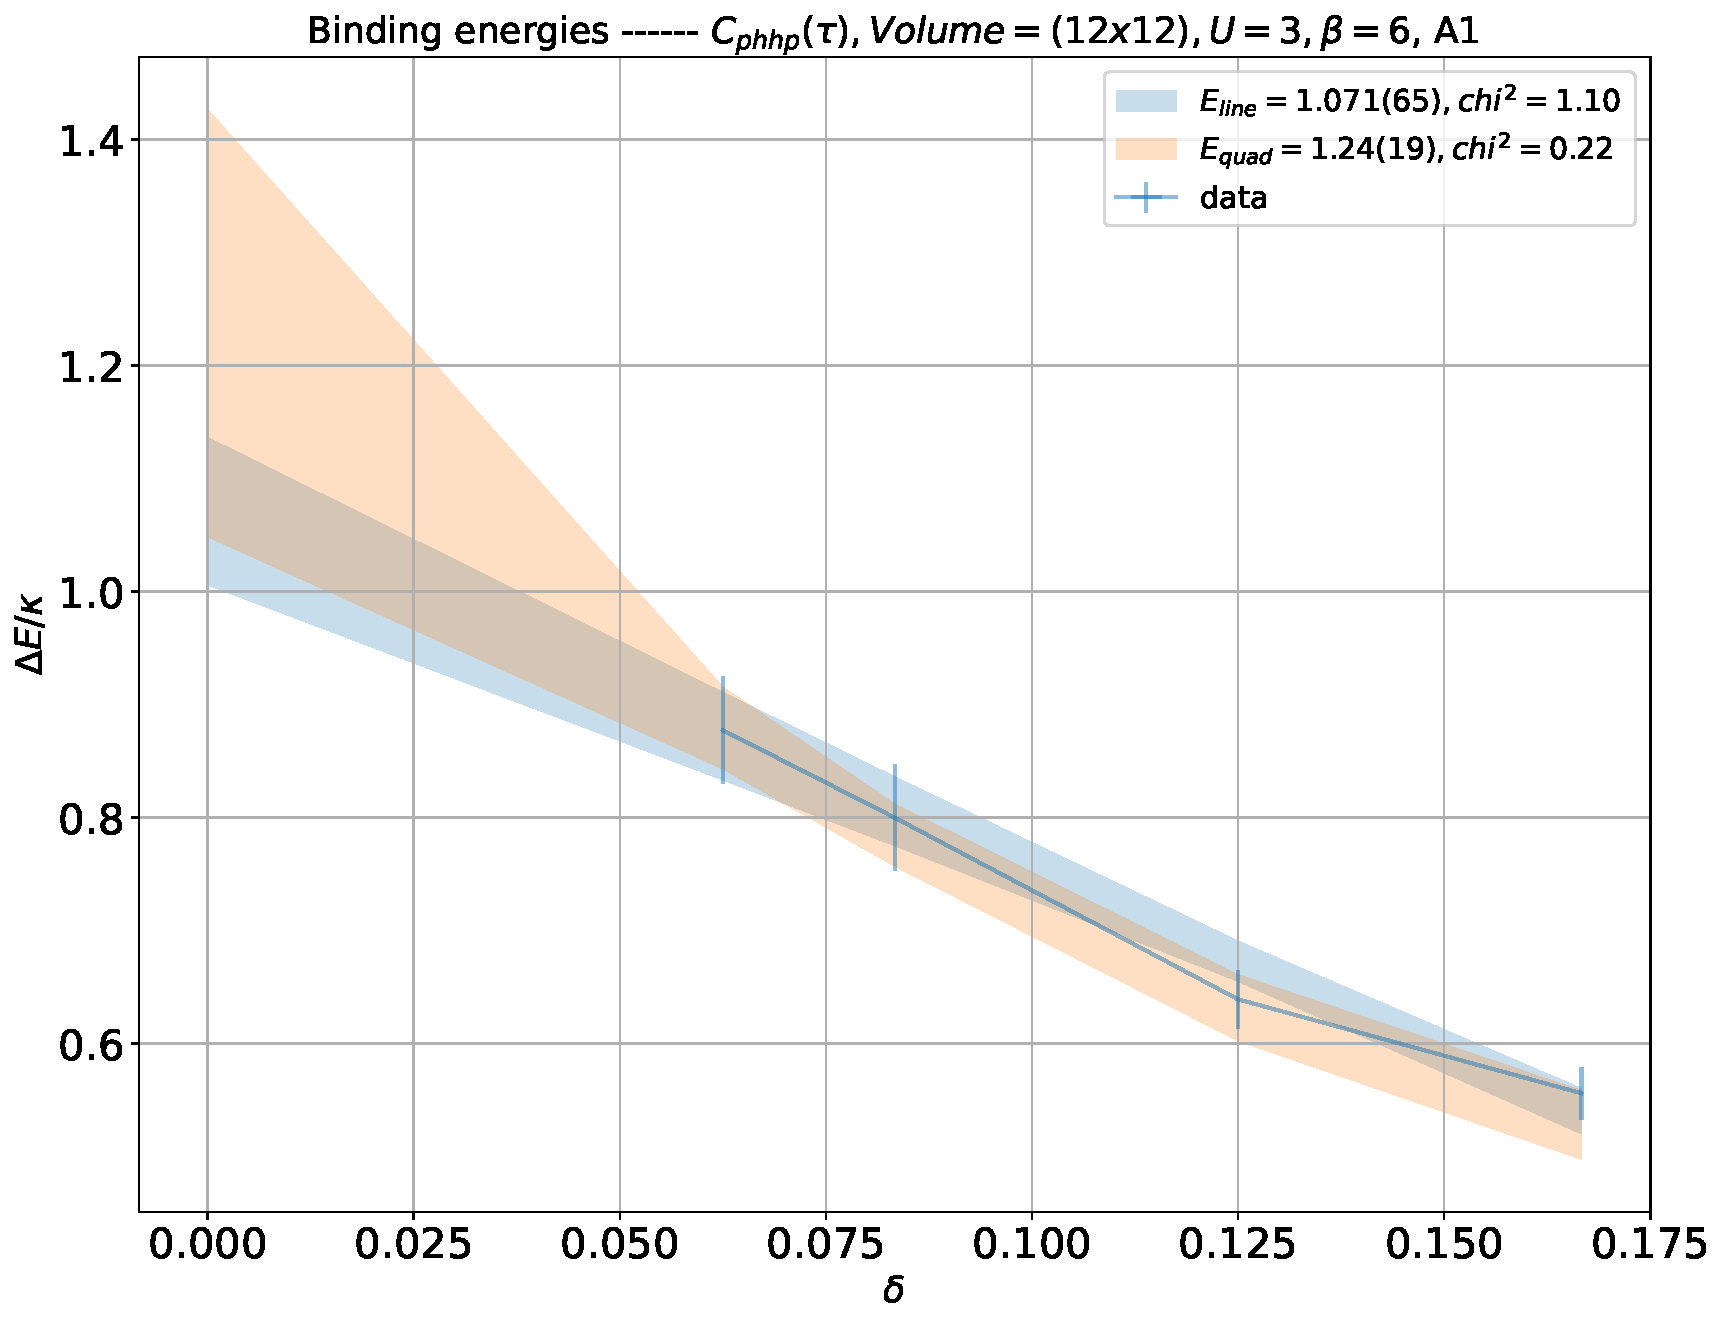
\includegraphics[width=\linewidth]{phhp-0-A1_12x12_U3_B6_cont.pdf}
  \end{subfigure}
  \begin{subfigure}{.5\textwidth}
      \centering
      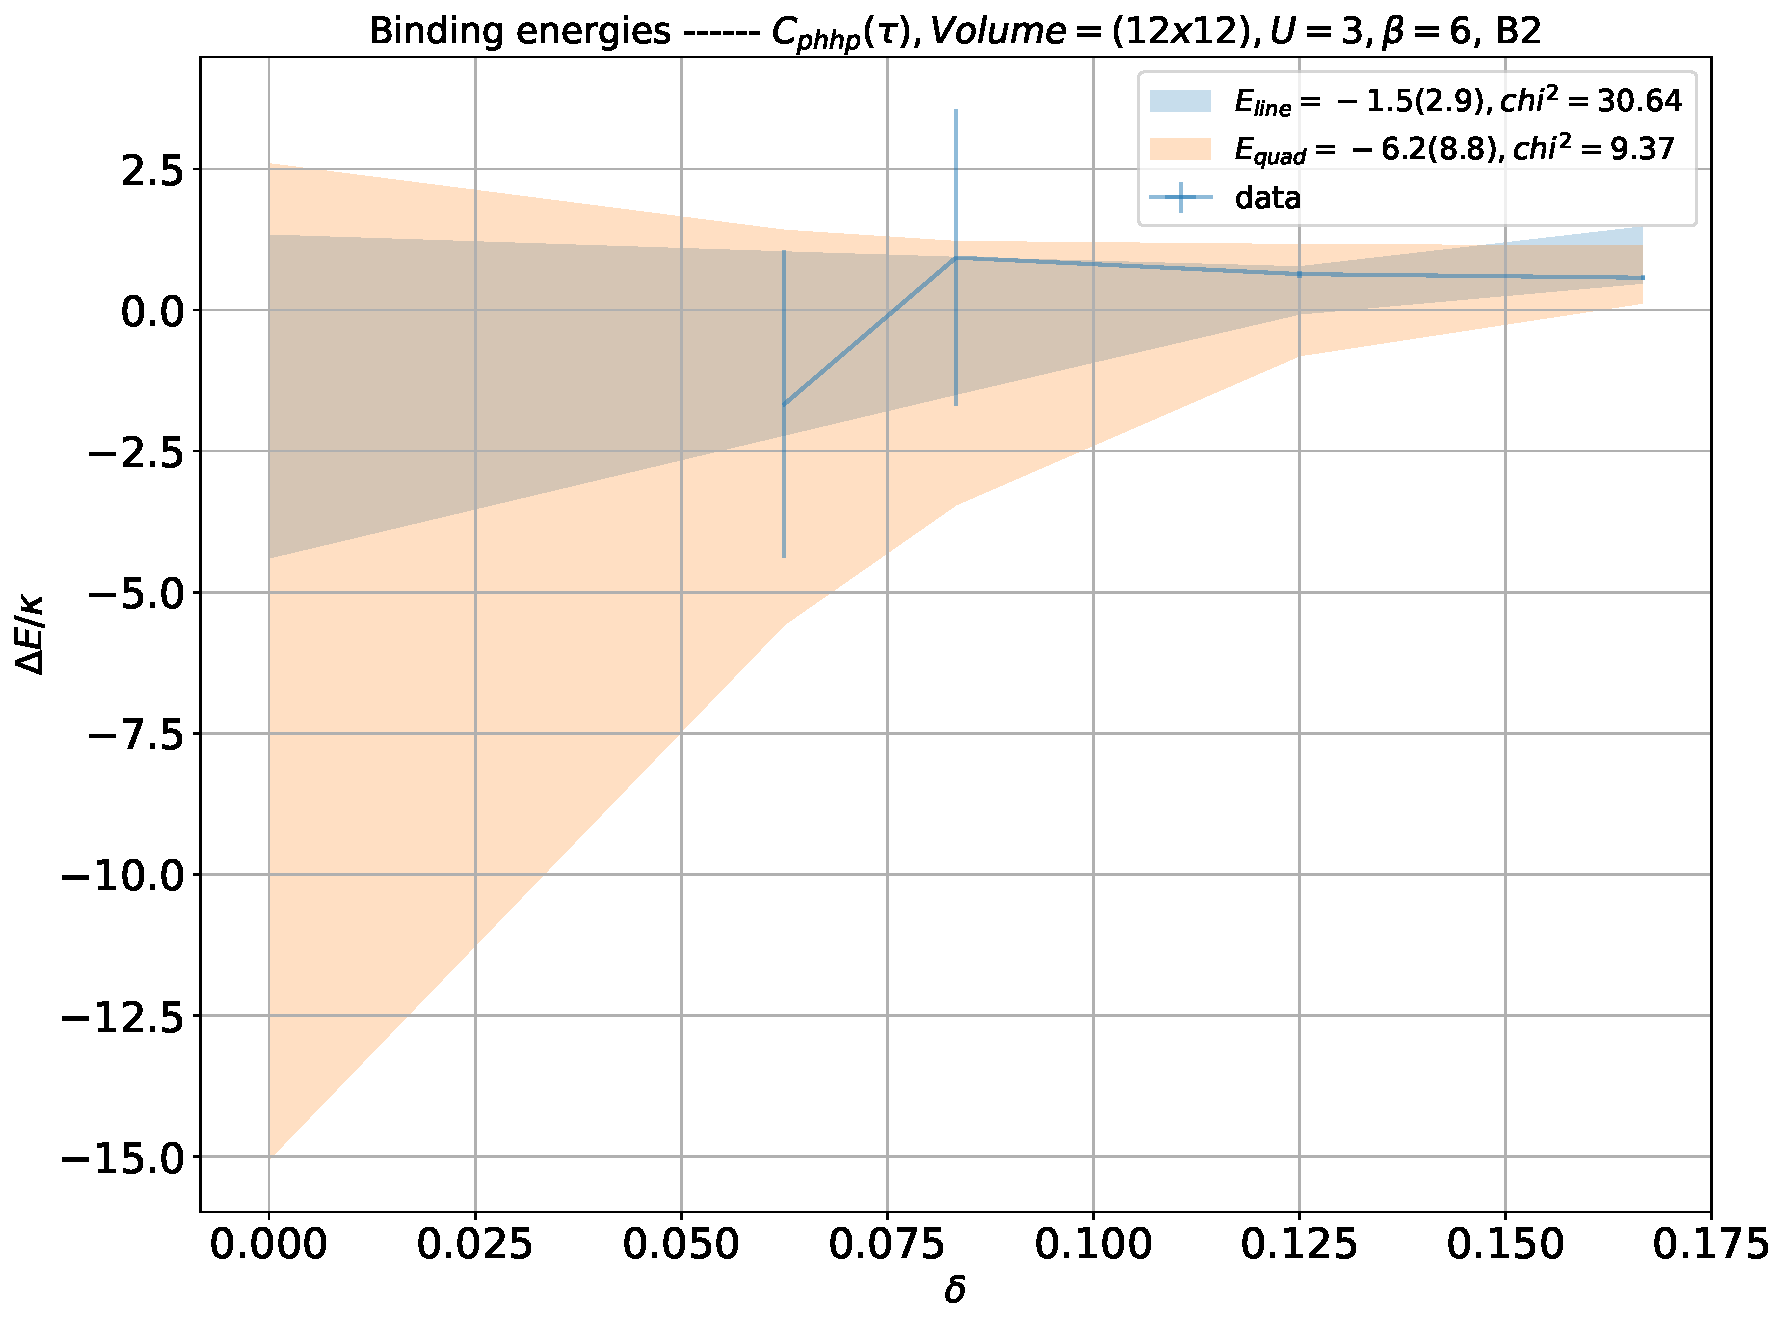
\includegraphics[width=\linewidth]{phhp-0-B2_12x12_U3_B6_cont.pdf}
  \end{subfigure}
  \caption{Binding energy extraction of the particle-hole pair at both irreducible representations, where we fit one- and two-body correlators for every $N_t$. This is followed by fitting a linear and a quadratic functions to the $\Delta E_{N_t}$ in order to extrapolate to the continuum limit ($N_t\to\infty$).}
  \label{fig:fig3}
\end{figure}

\begin{figure}
  \begin{subfigure}{.5\textwidth}
    \centering
    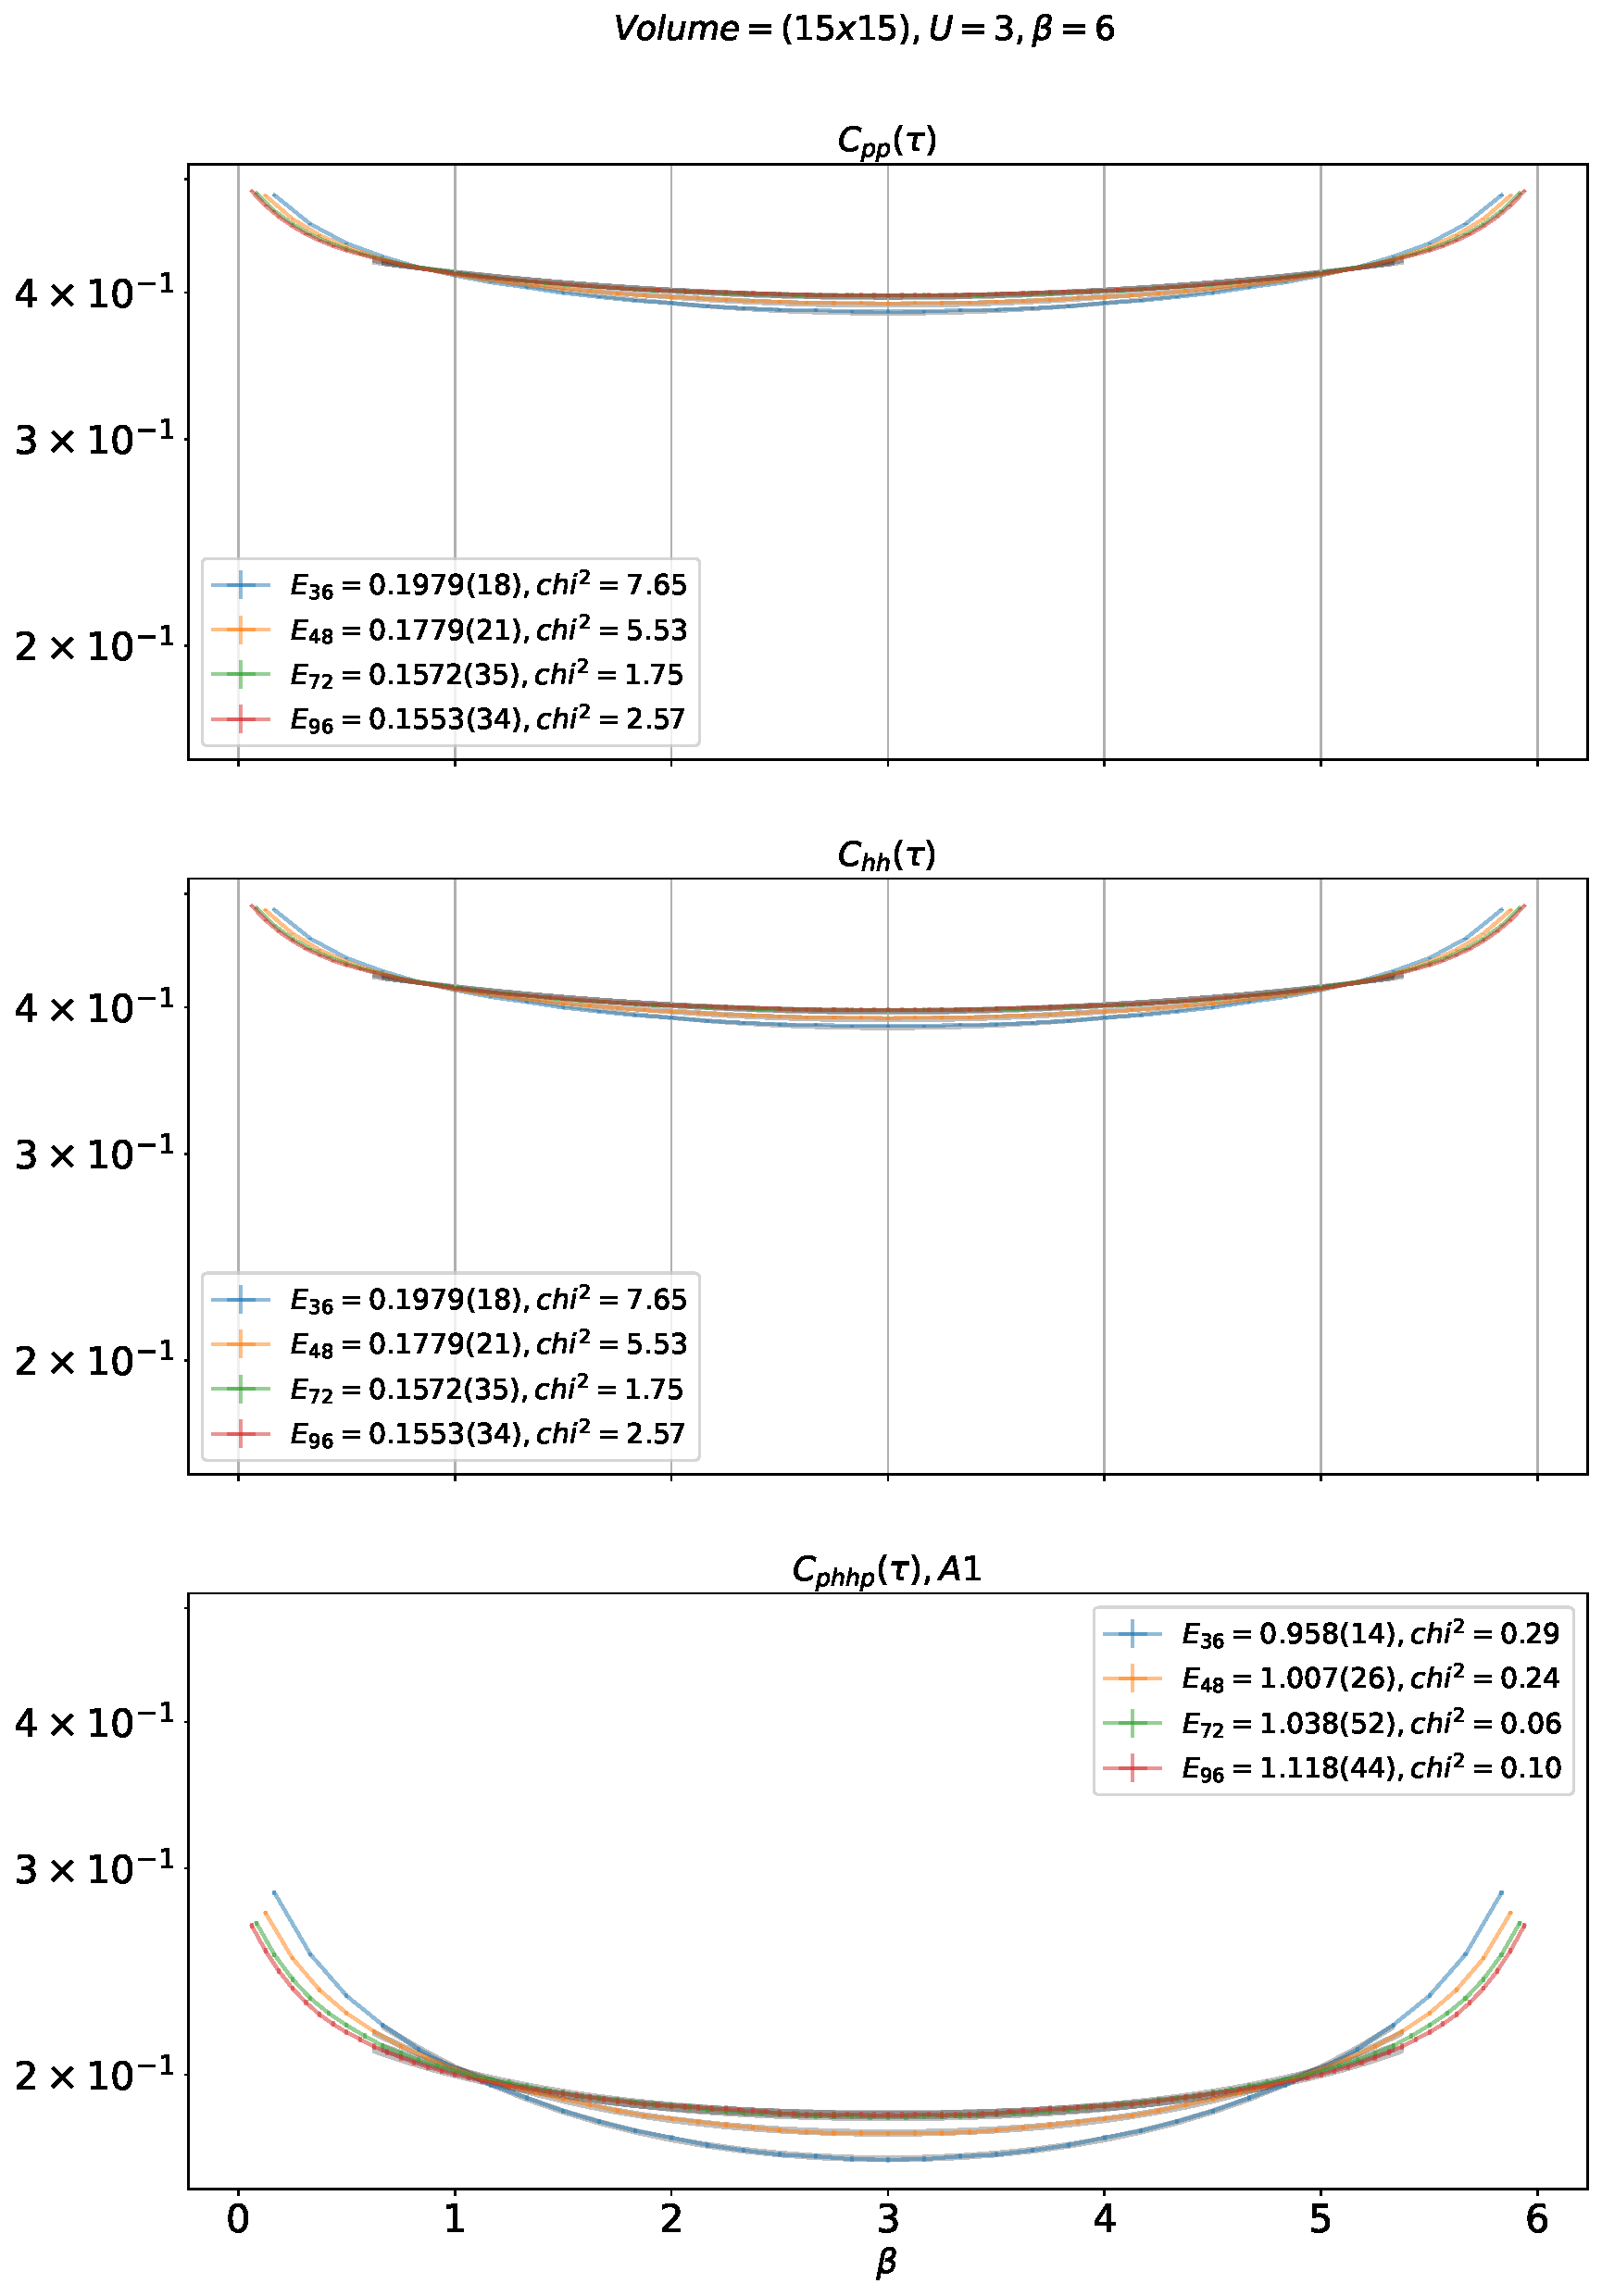
\includegraphics[width=\linewidth]{phhp-0-A1_15x15_U3_B6.pdf}
  \end{subfigure}%
  \begin{subfigure}{.5\textwidth}
    \centering
    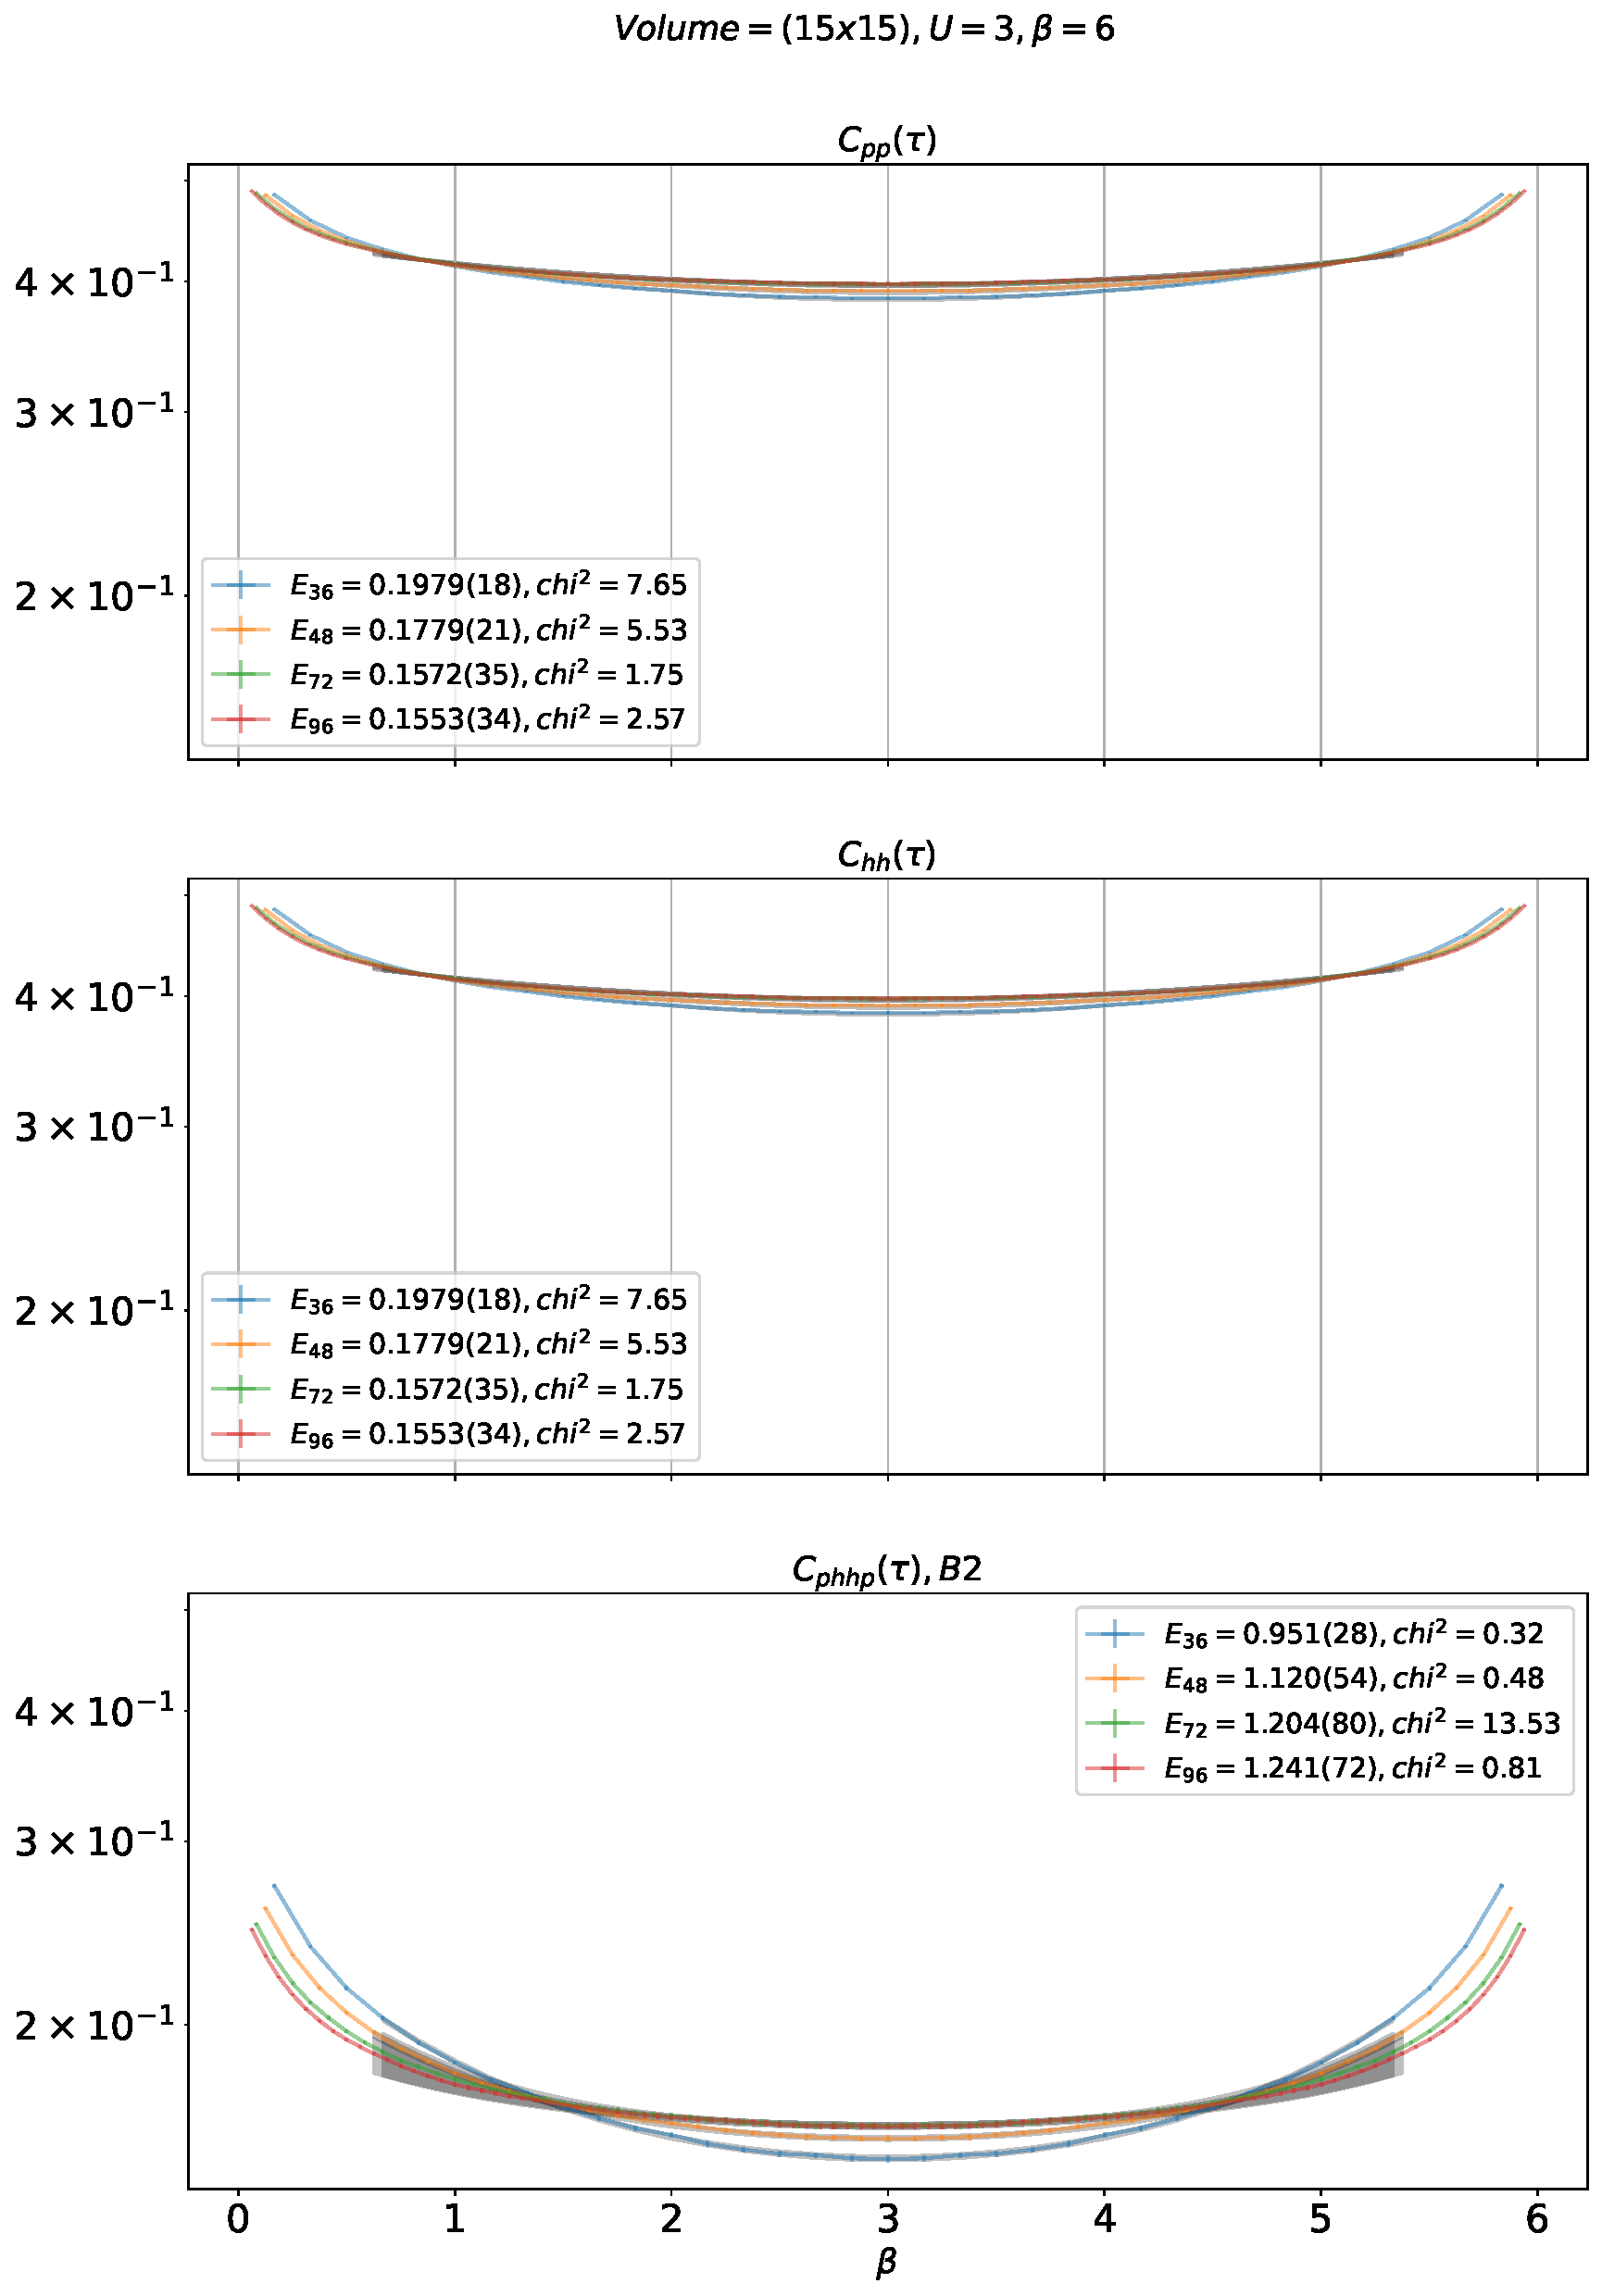
\includegraphics[width=\linewidth]{phhp-0-B2_15x15_U3_B6.pdf}
  \end{subfigure}
  \begin{subfigure}{.5\textwidth}
      \centering
      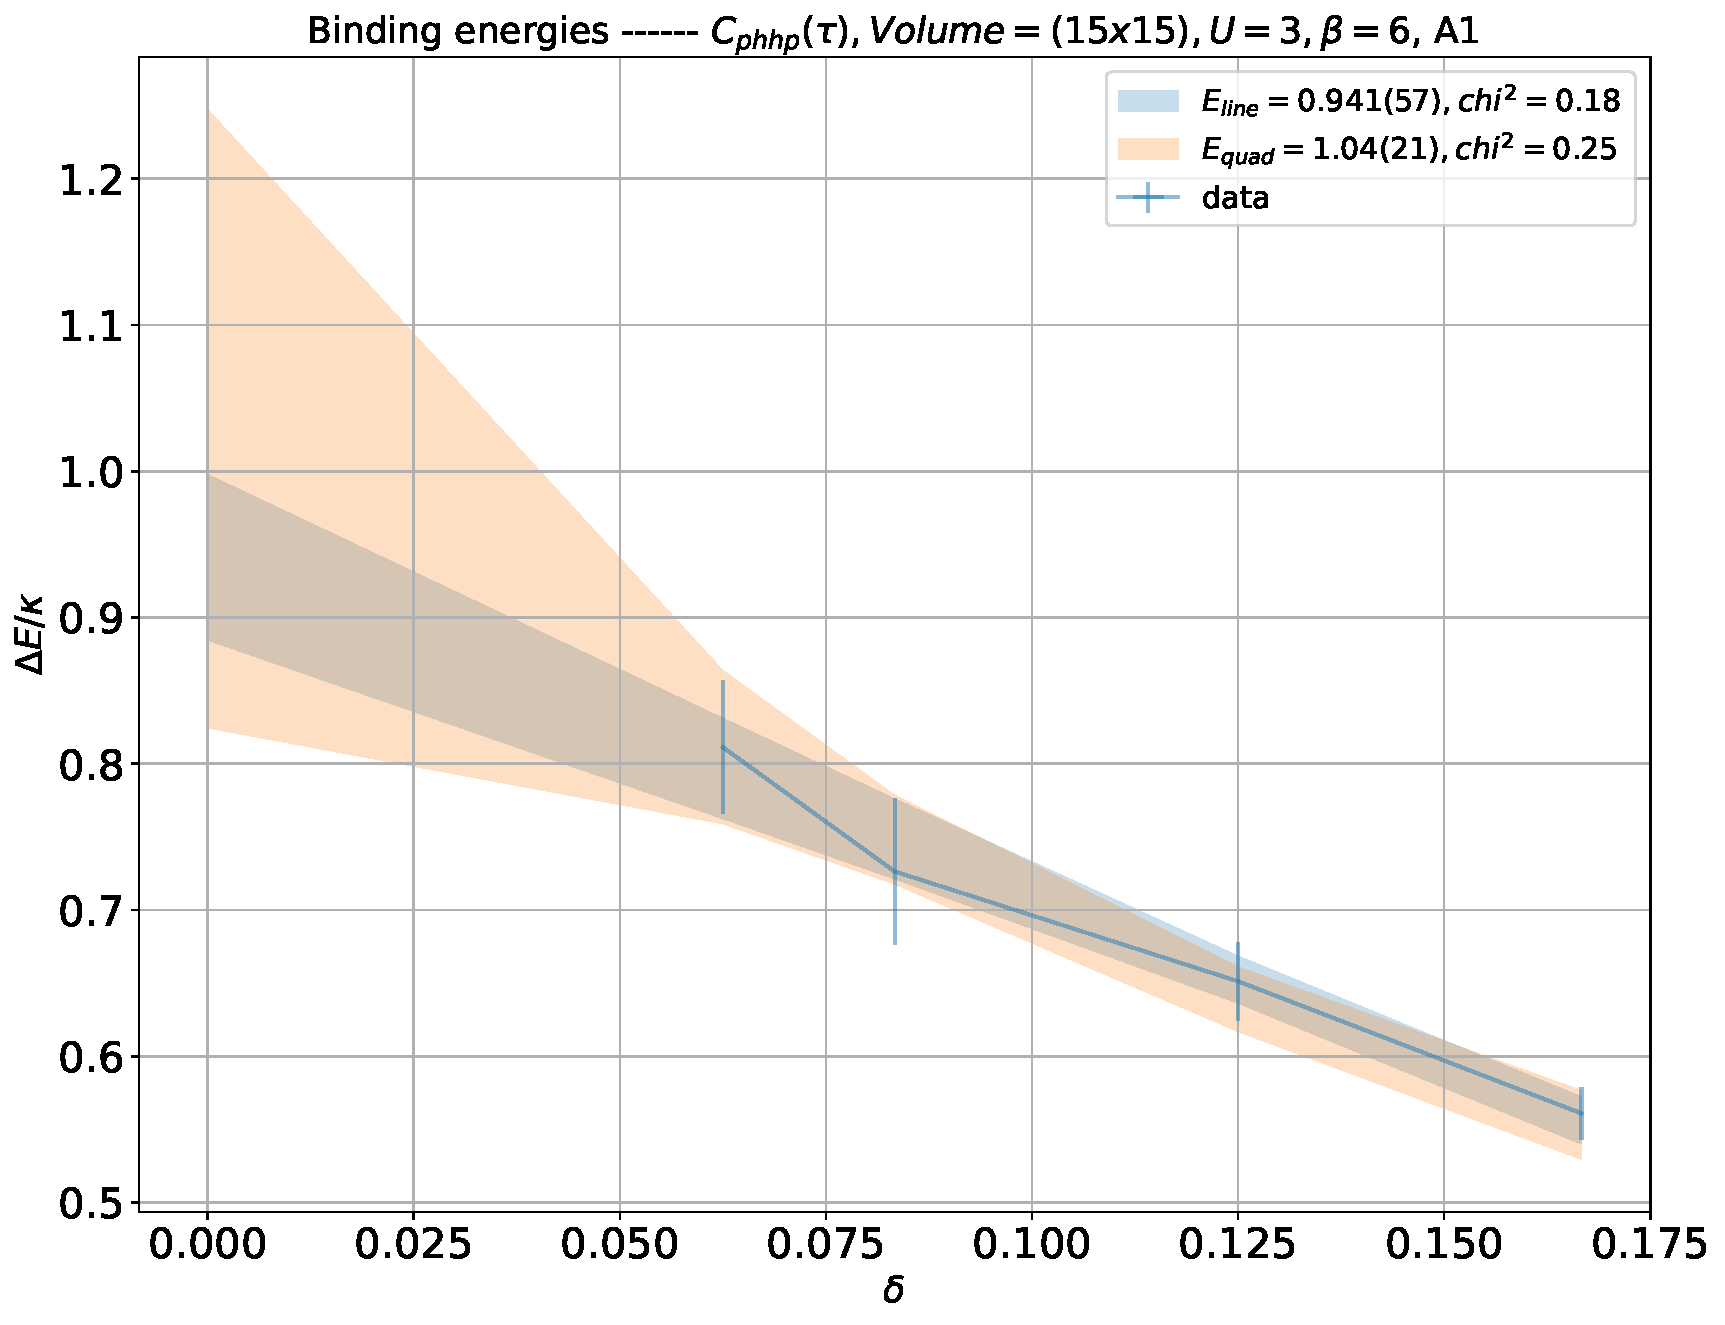
\includegraphics[width=\linewidth]{phhp-0-A1_15x15_U3_B6_cont.pdf}
  \end{subfigure}
  \begin{subfigure}{.5\textwidth}
      \centering
      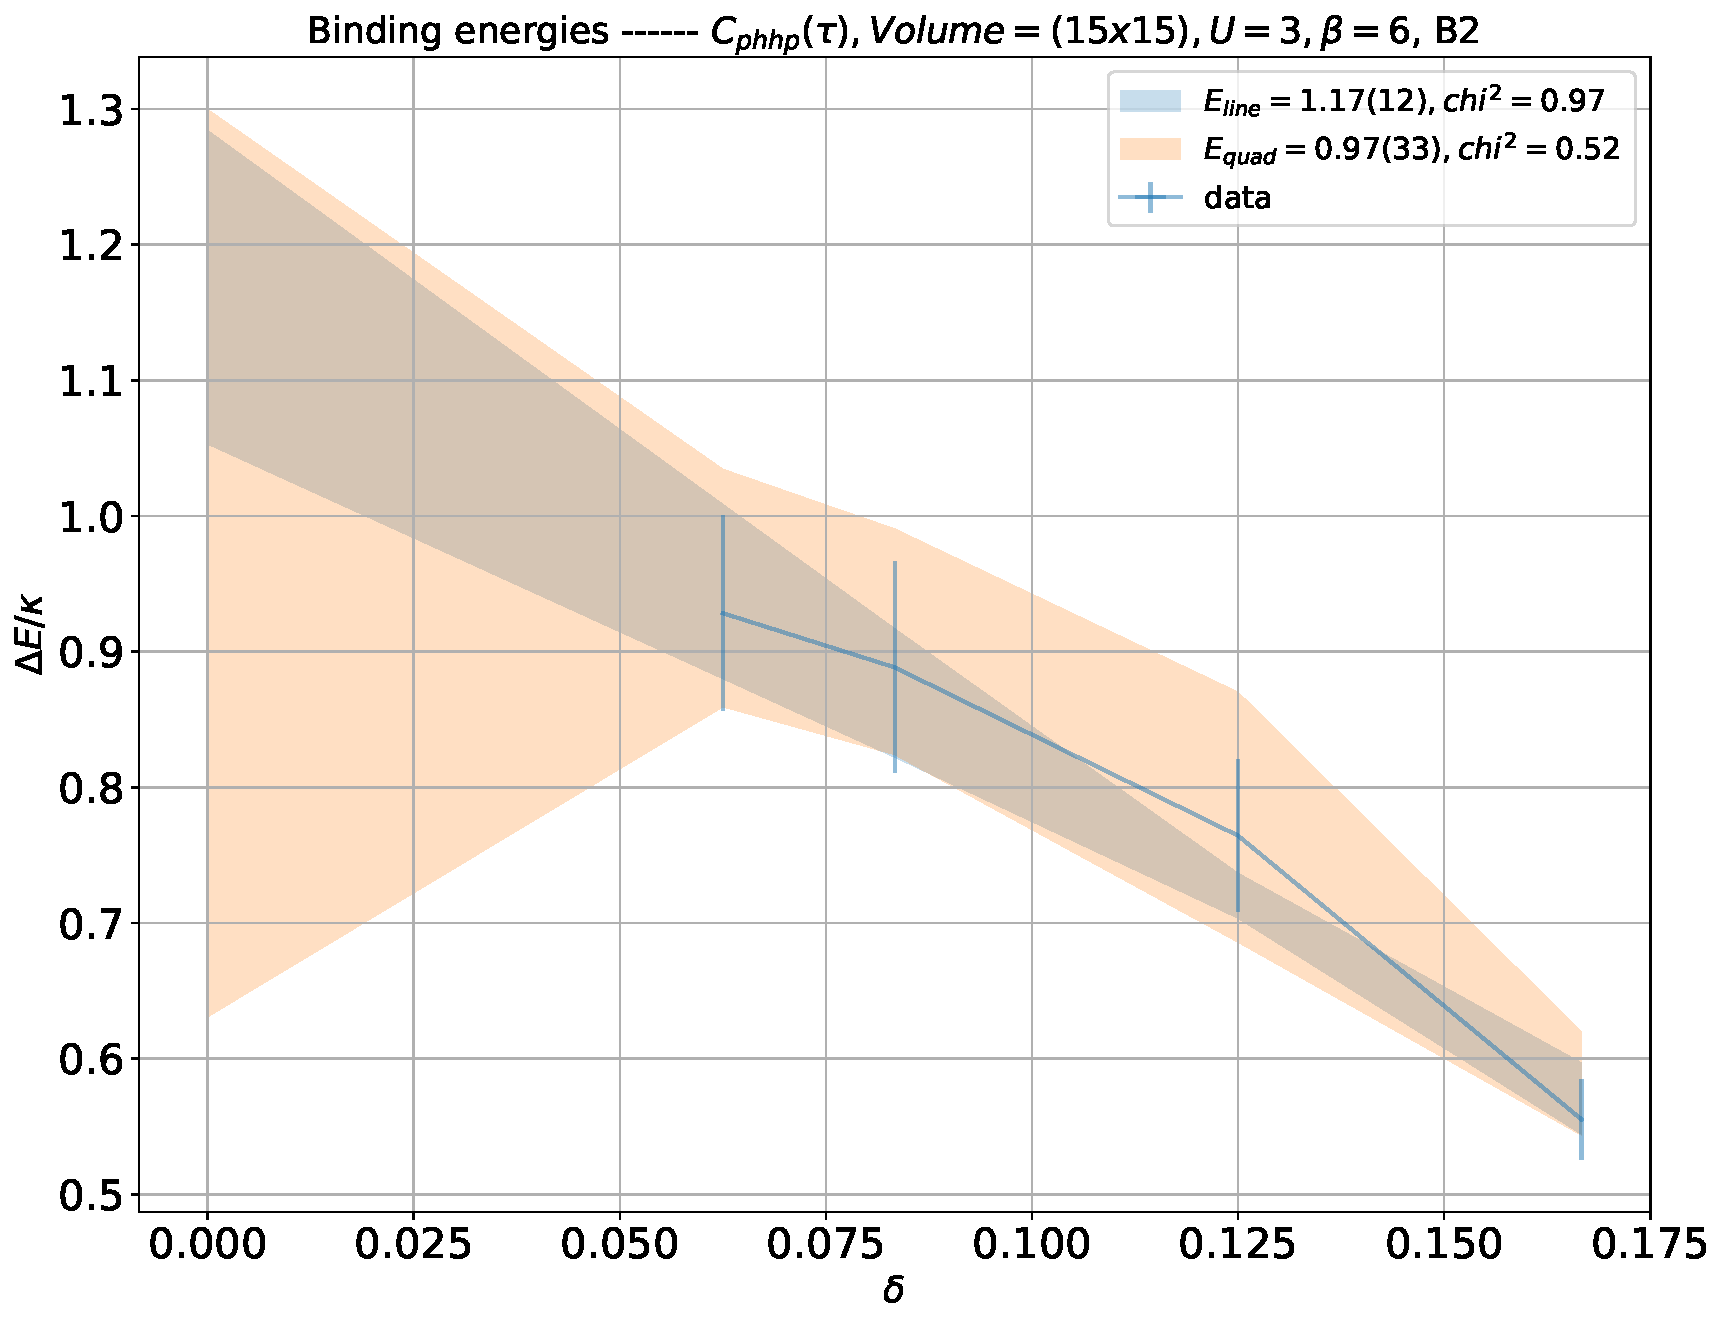
\includegraphics[width=\linewidth]{phhp-0-B2_15x15_U3_B6_cont.pdf}
  \end{subfigure}
  \caption{Binding energy extraction of the particle-hole pair at both irreducible representations, where we fit one- and two-body correlators for every $N_t$. This is followed by fitting a linear and a quadratic functions to the $\Delta E_{N_t}$ in order to extrapolate to the continuum limit ($N_t\to\infty$).}
  \label{fig:fig4}
\end{figure}

\begin{figure}
  \begin{subfigure}{.5\textwidth}
    \centering
    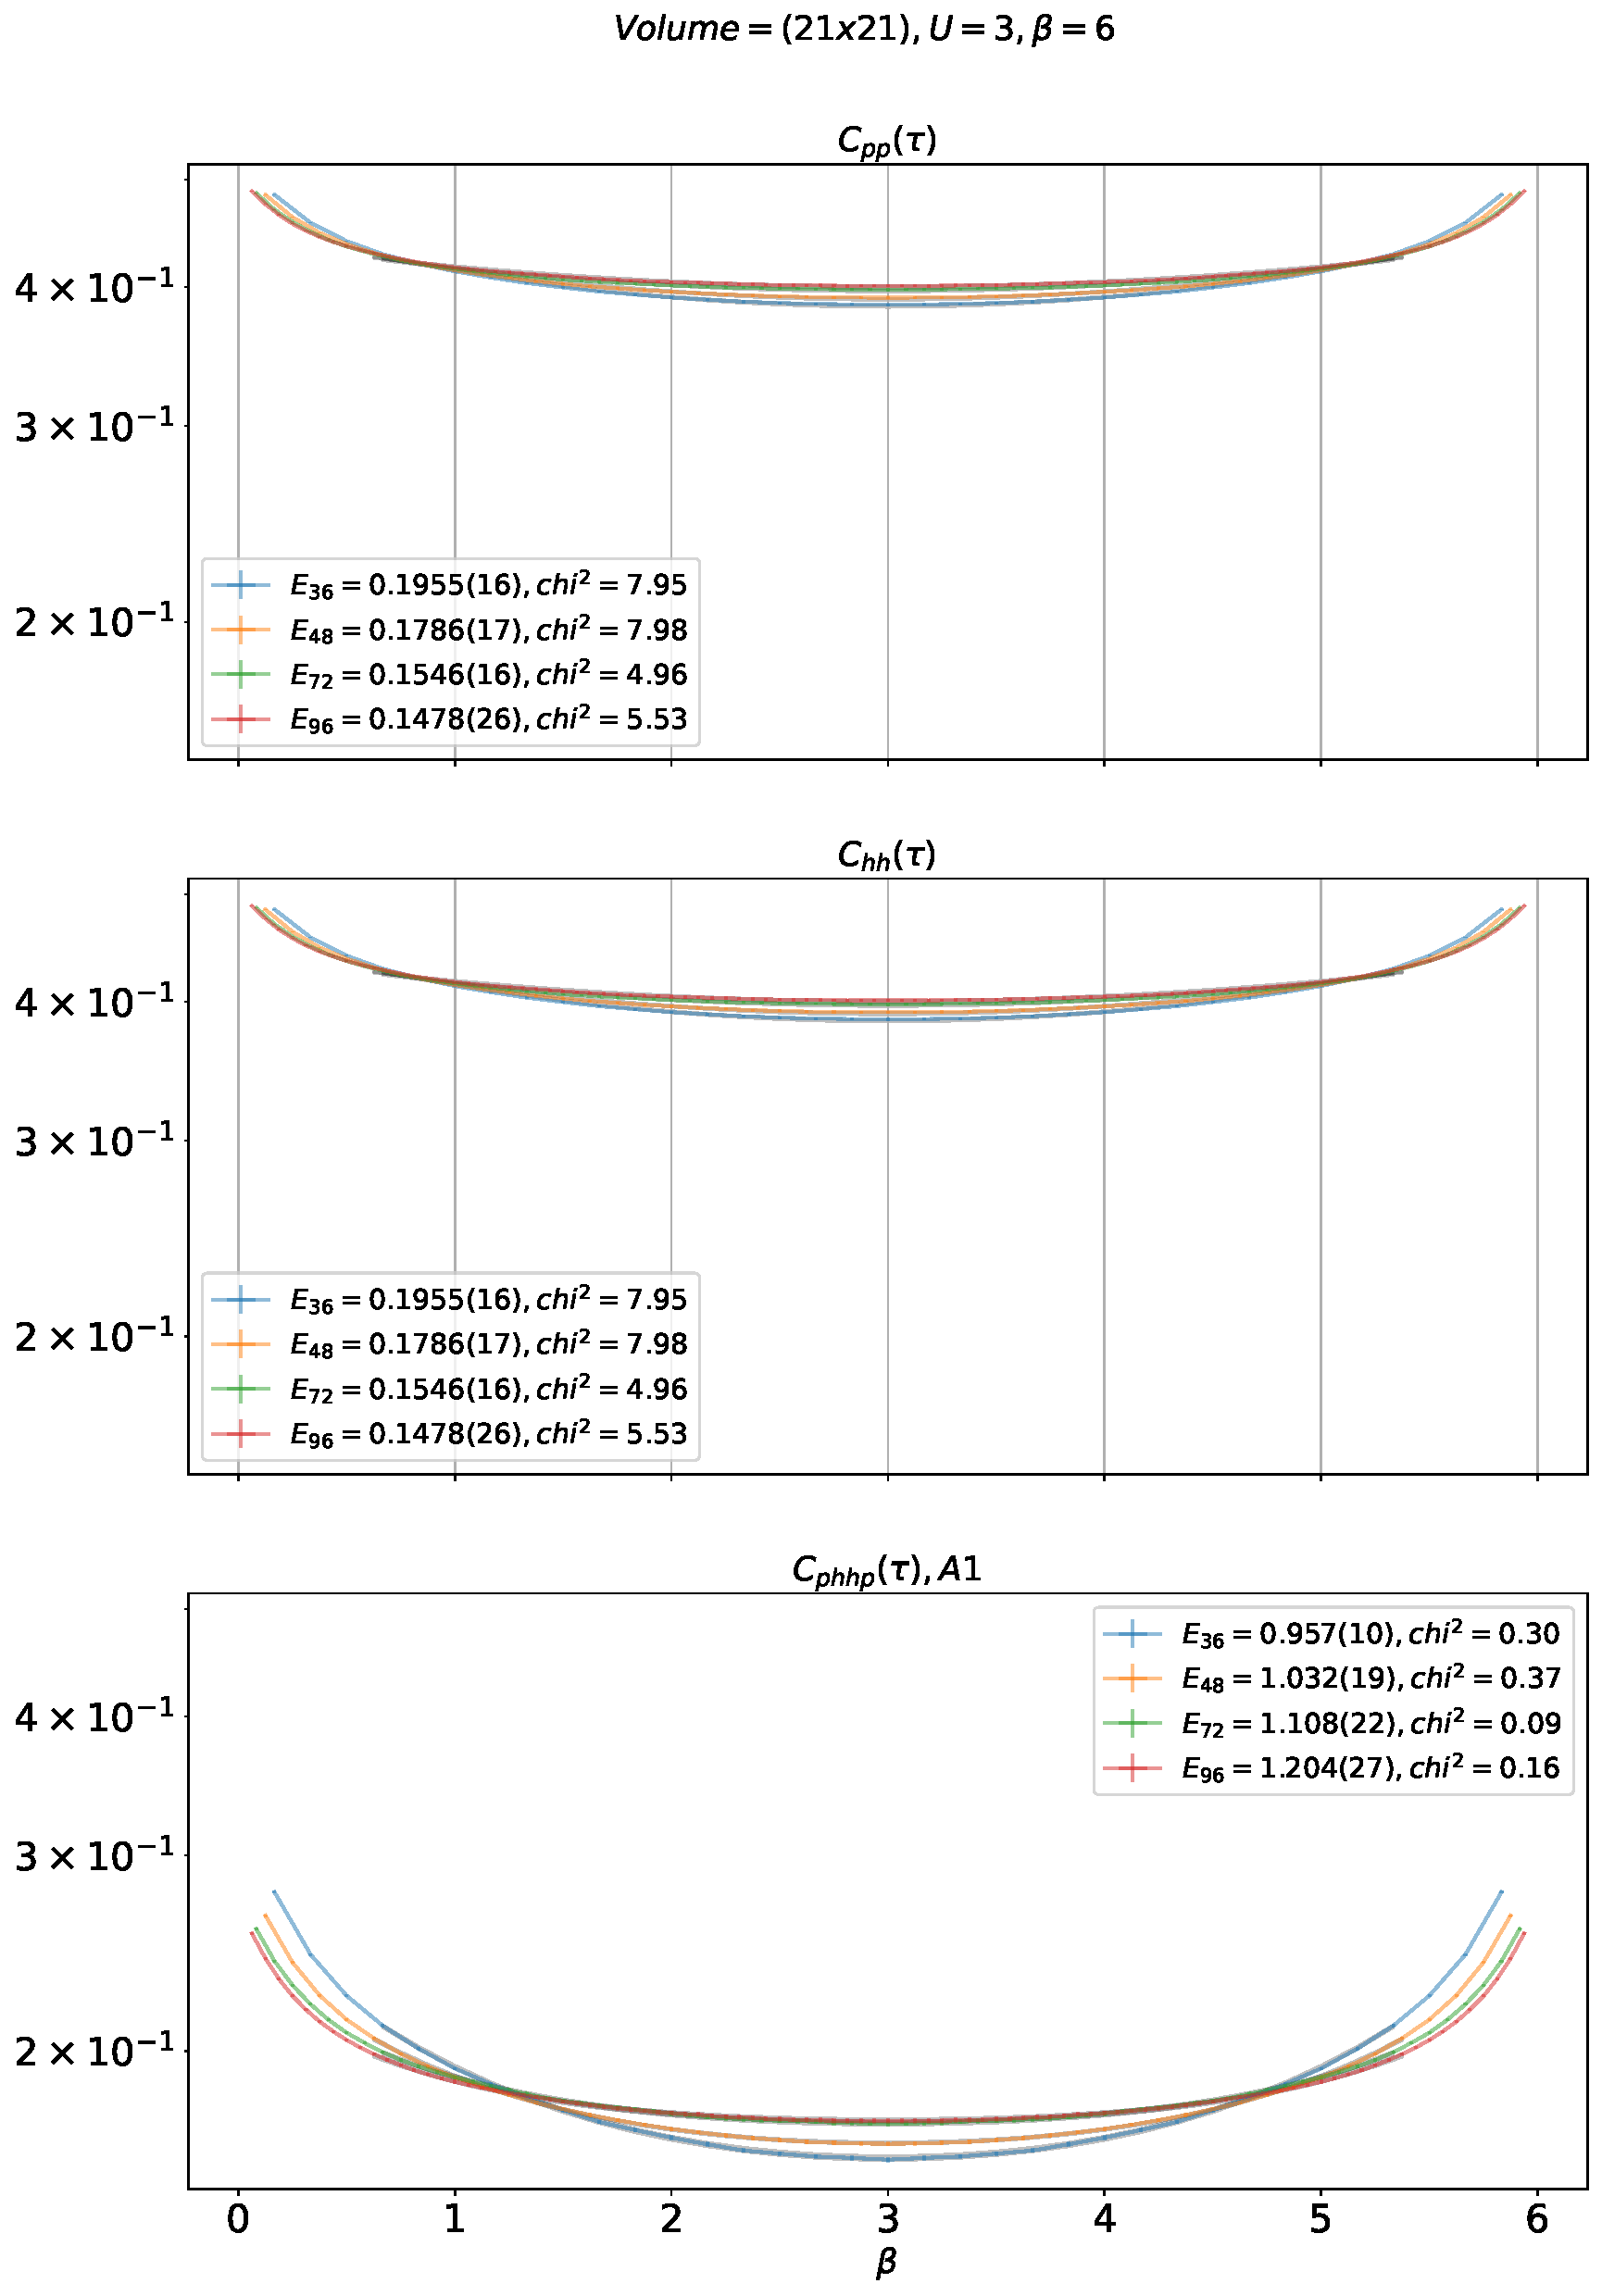
\includegraphics[width=\linewidth]{phhp-0-A1_21x21_U3_B6.pdf}
  \end{subfigure}%
  \begin{subfigure}{.5\textwidth}
    \centering
    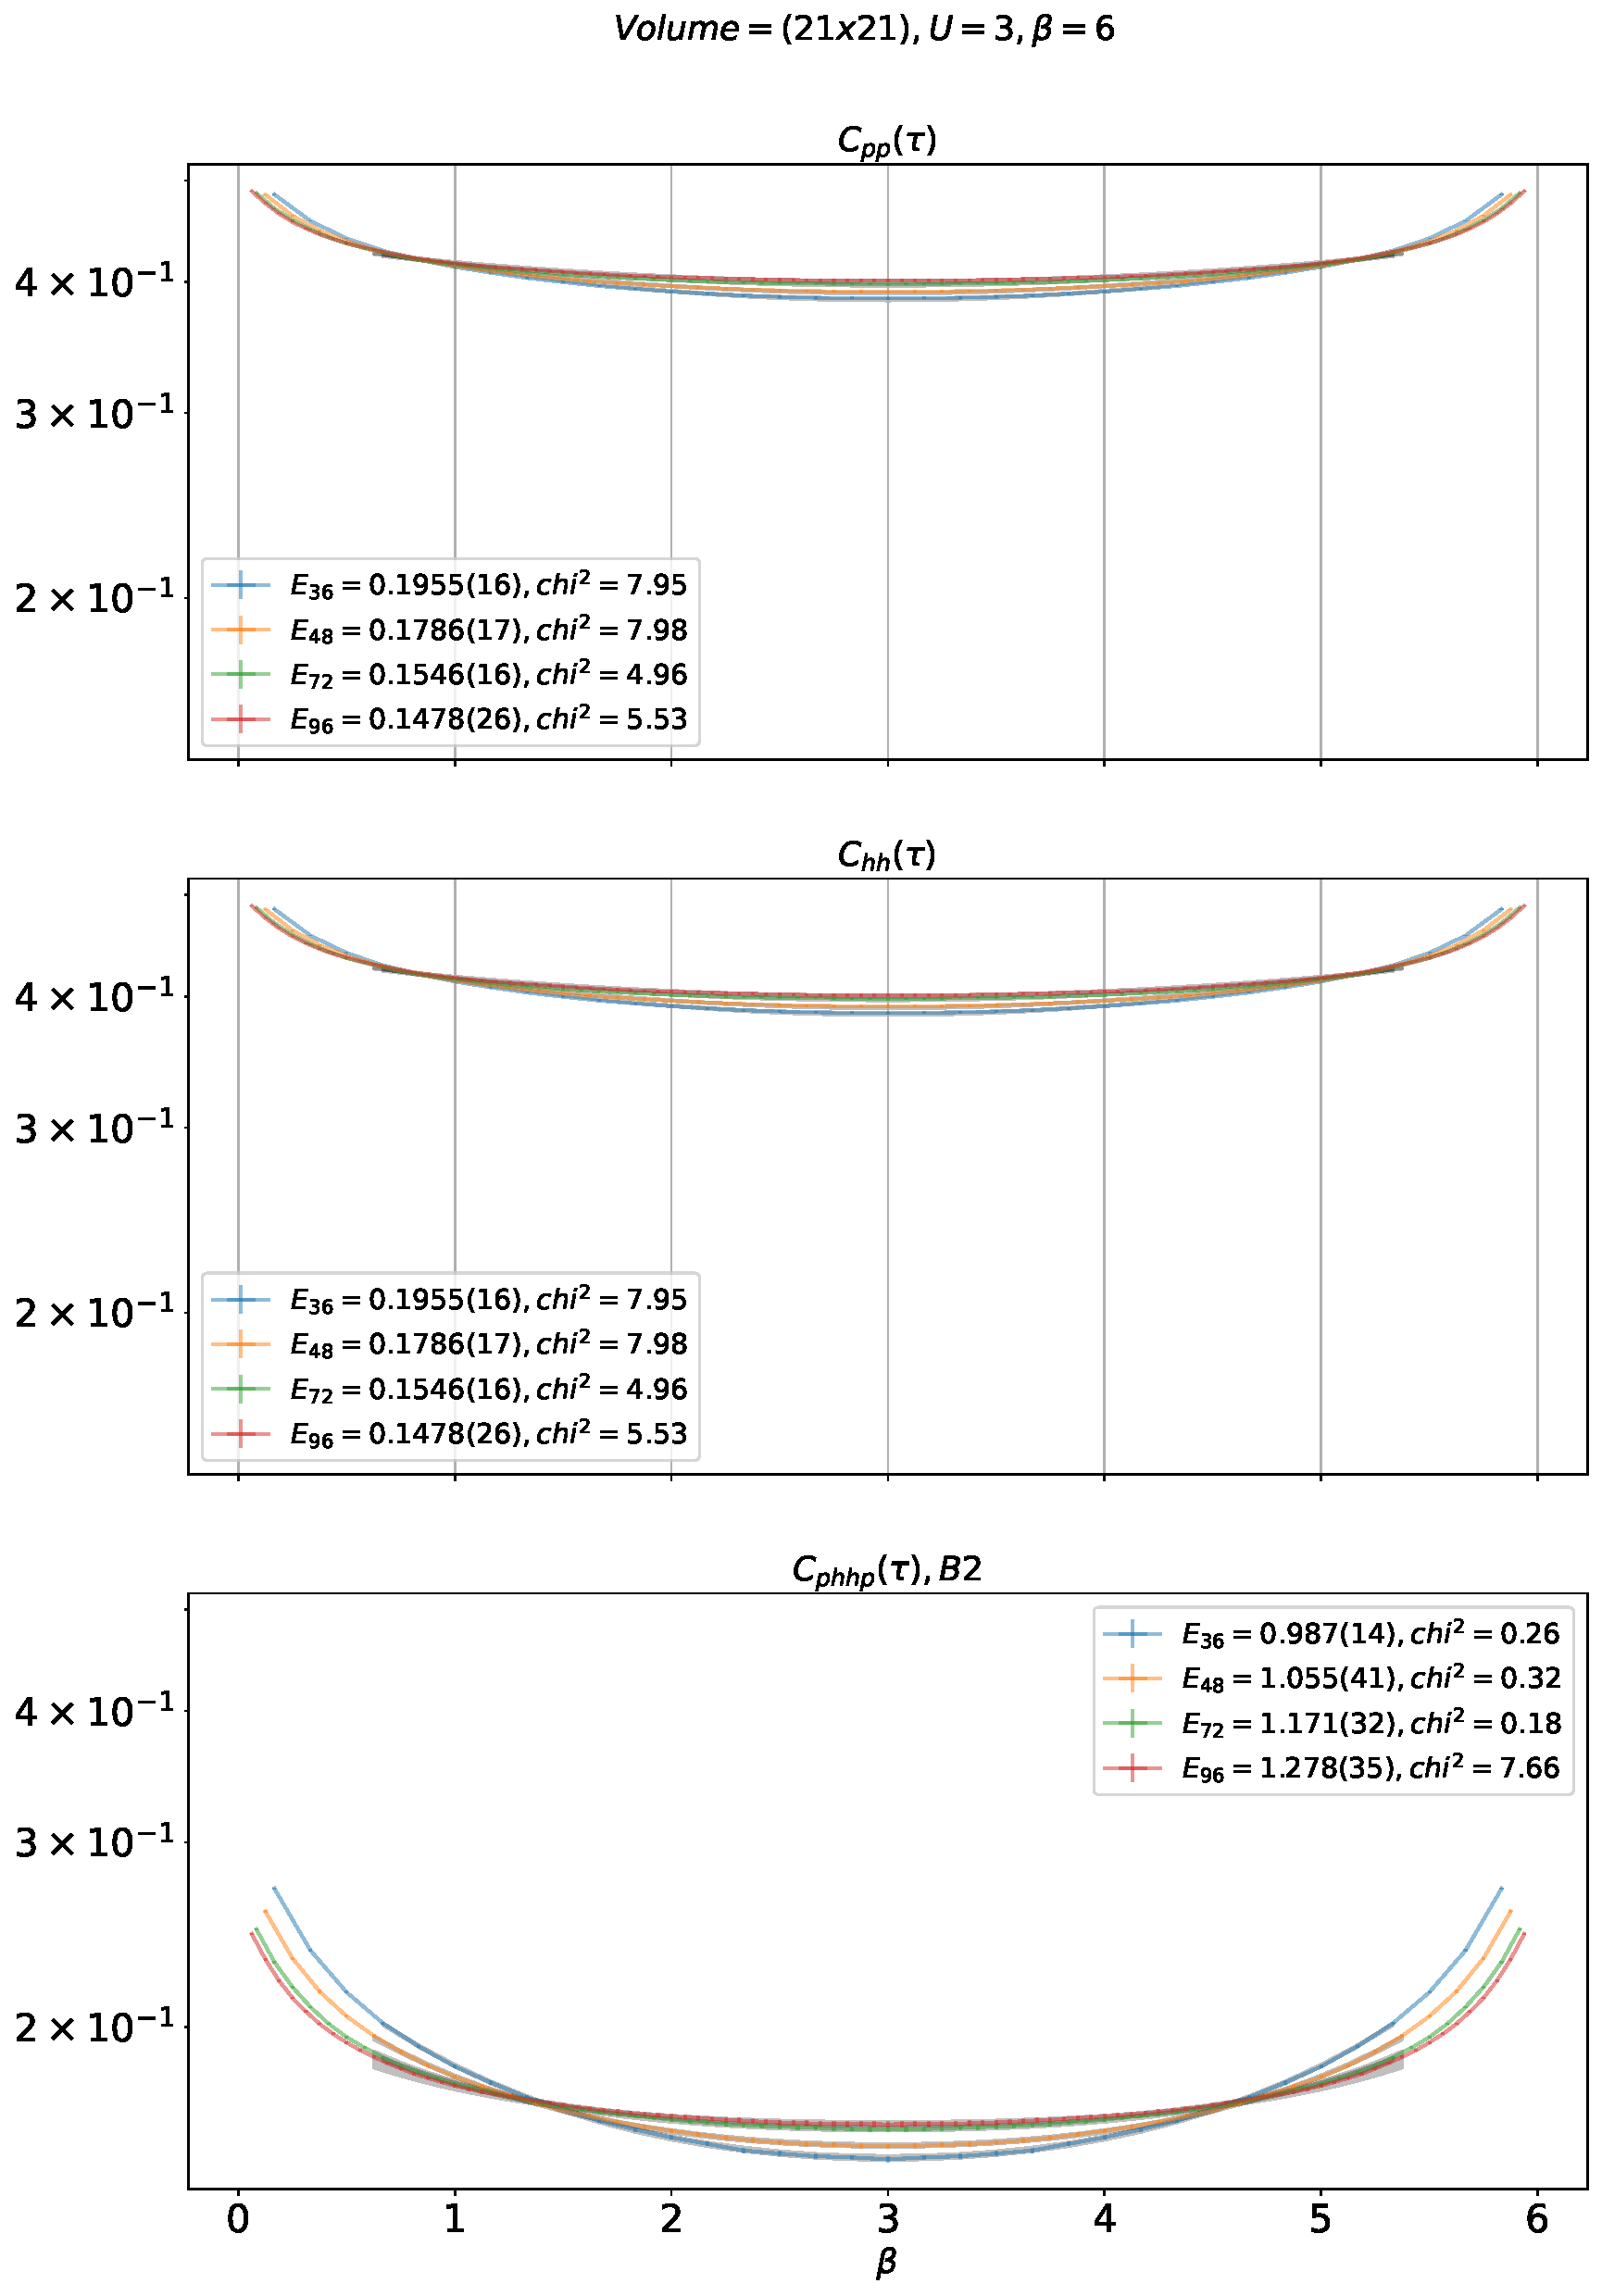
\includegraphics[width=\linewidth]{phhp-0-B2_21x21_U3_B6.pdf}
  \end{subfigure}
  \begin{subfigure}{.5\textwidth}
      \centering
      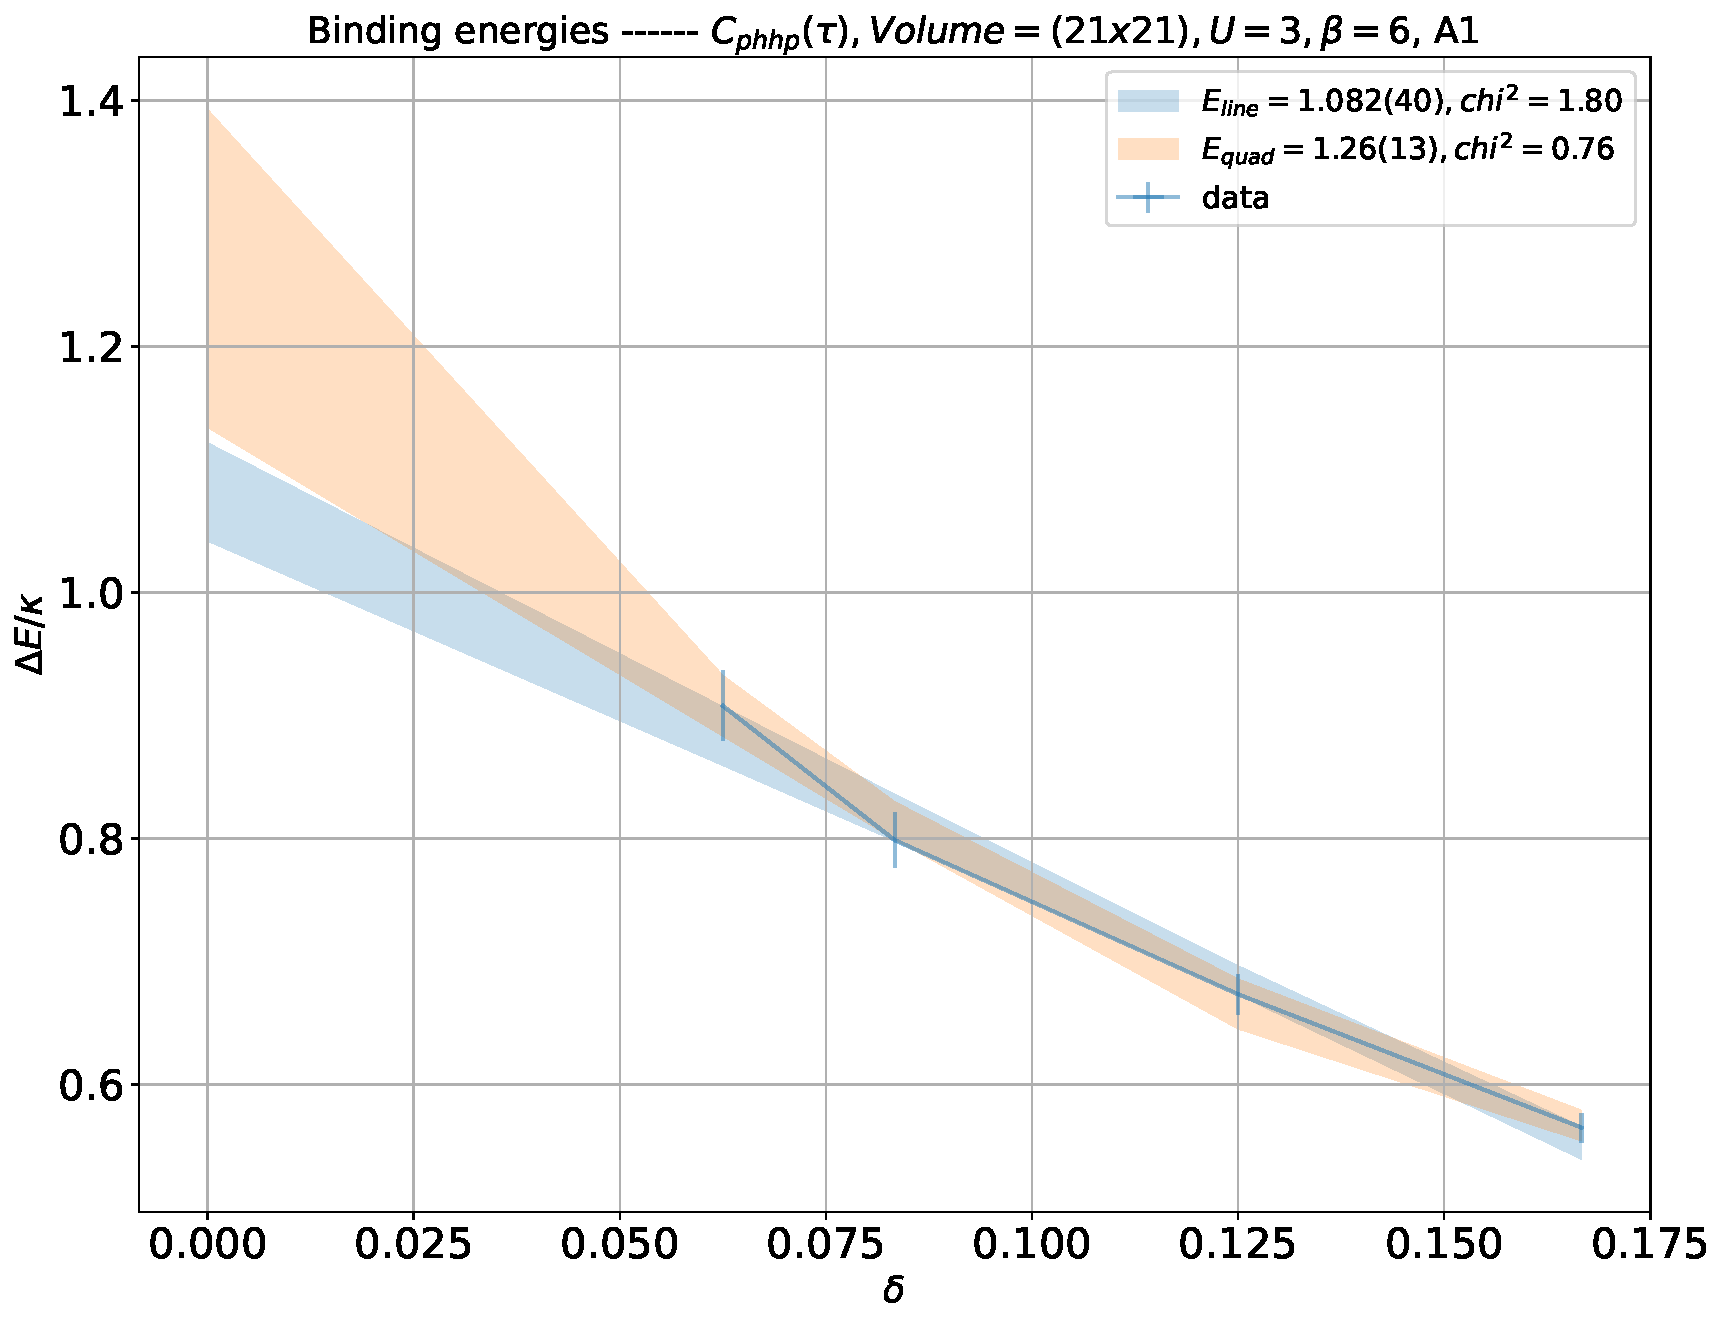
\includegraphics[width=\linewidth]{phhp-0-A1_21x21_U3_B6_cont.pdf}
  \end{subfigure}
  \begin{subfigure}{.5\textwidth}
      \centering
      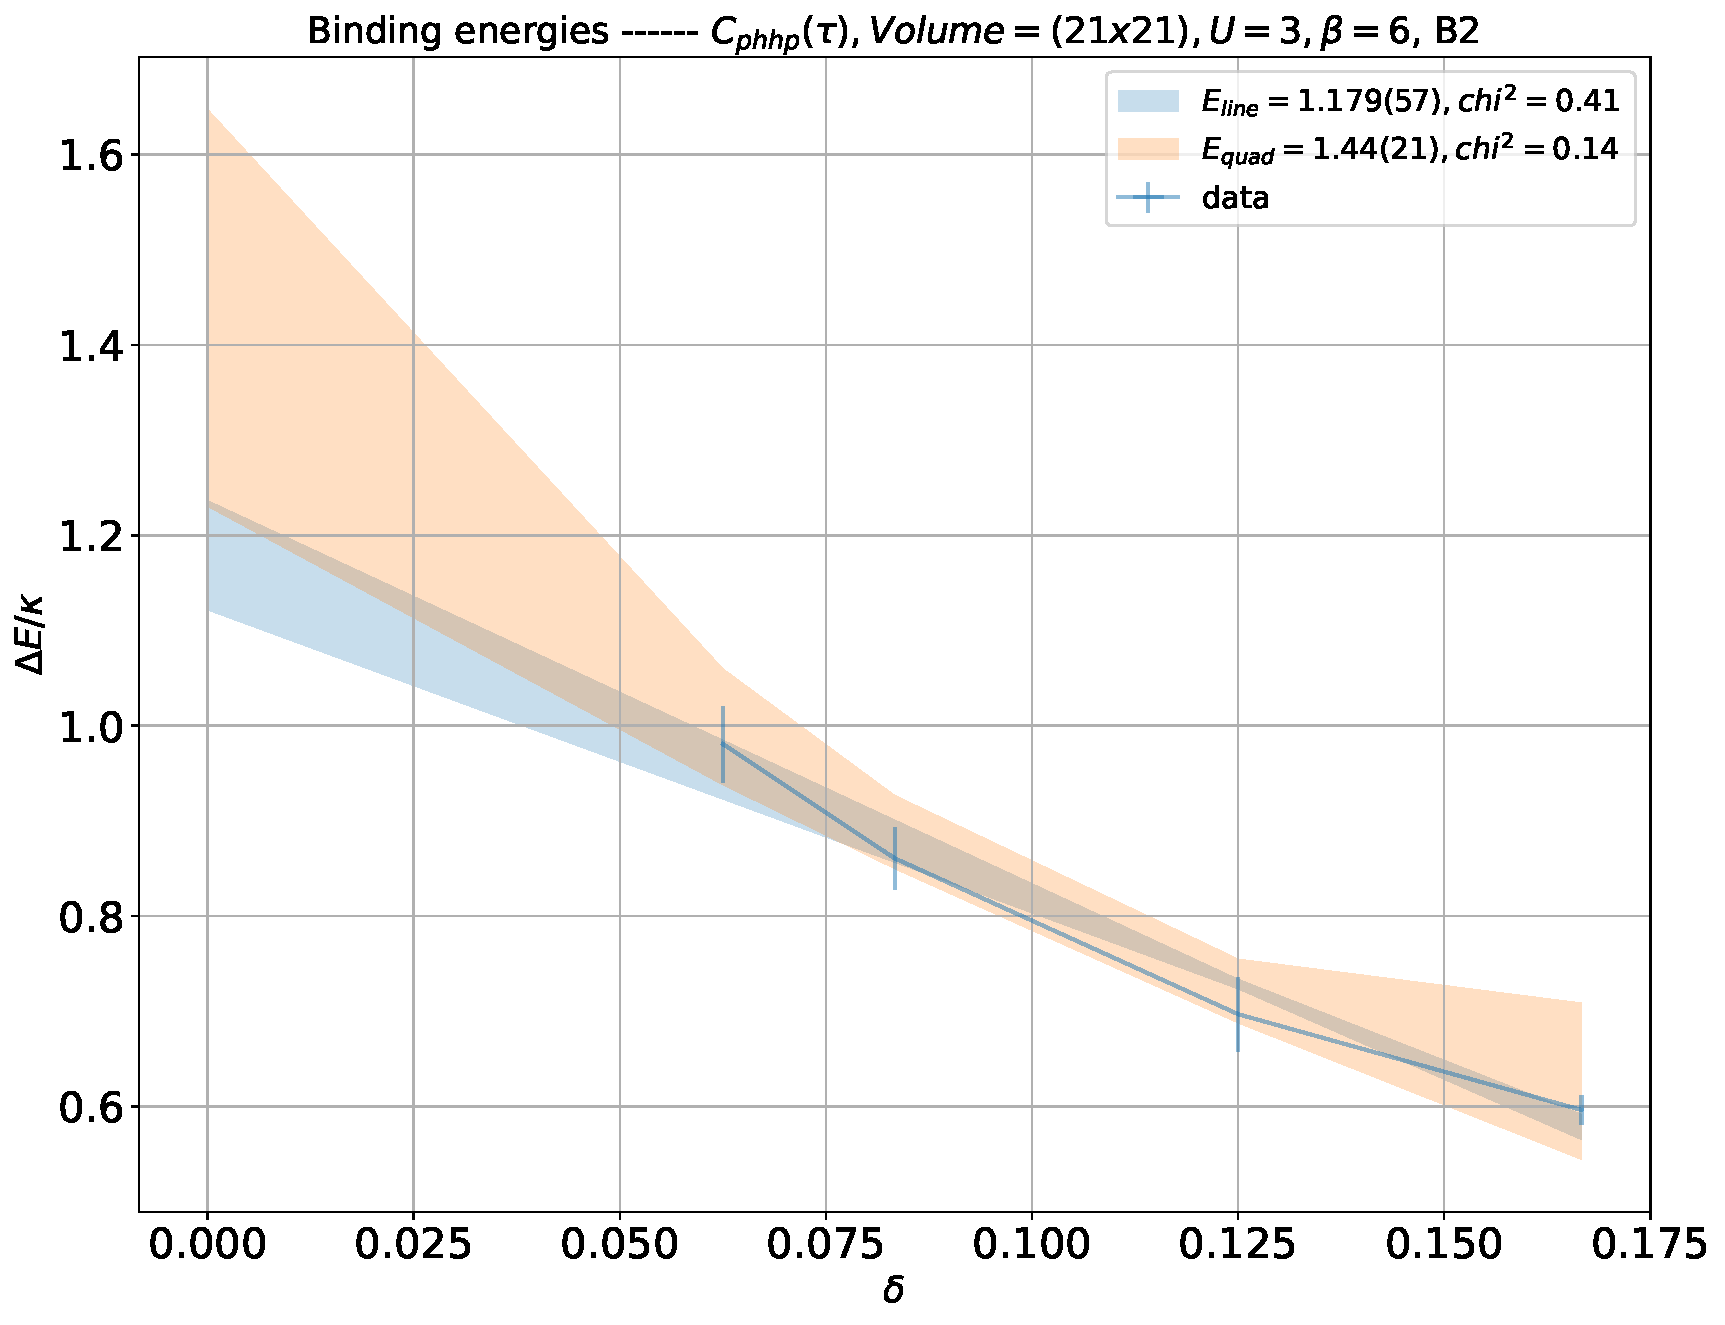
\includegraphics[width=\linewidth]{phhp-0-B2_21x21_U3_B6_cont.pdf}
  \end{subfigure}
  \caption{Binding energy extraction of the particle-hole pair at both irreducible representations, where we fit one- and two-body correlators for every $N_t$. This is followed by fitting a linear and a quadratic functions to the $\Delta E_{N_t}$ in order to extrapolate to the continuum limit ($N_t\to\infty$).}
  \label{fig:fig5}
\end{figure}

\begin{figure}
  \begin{subfigure}{.5\textwidth}
    \centering
    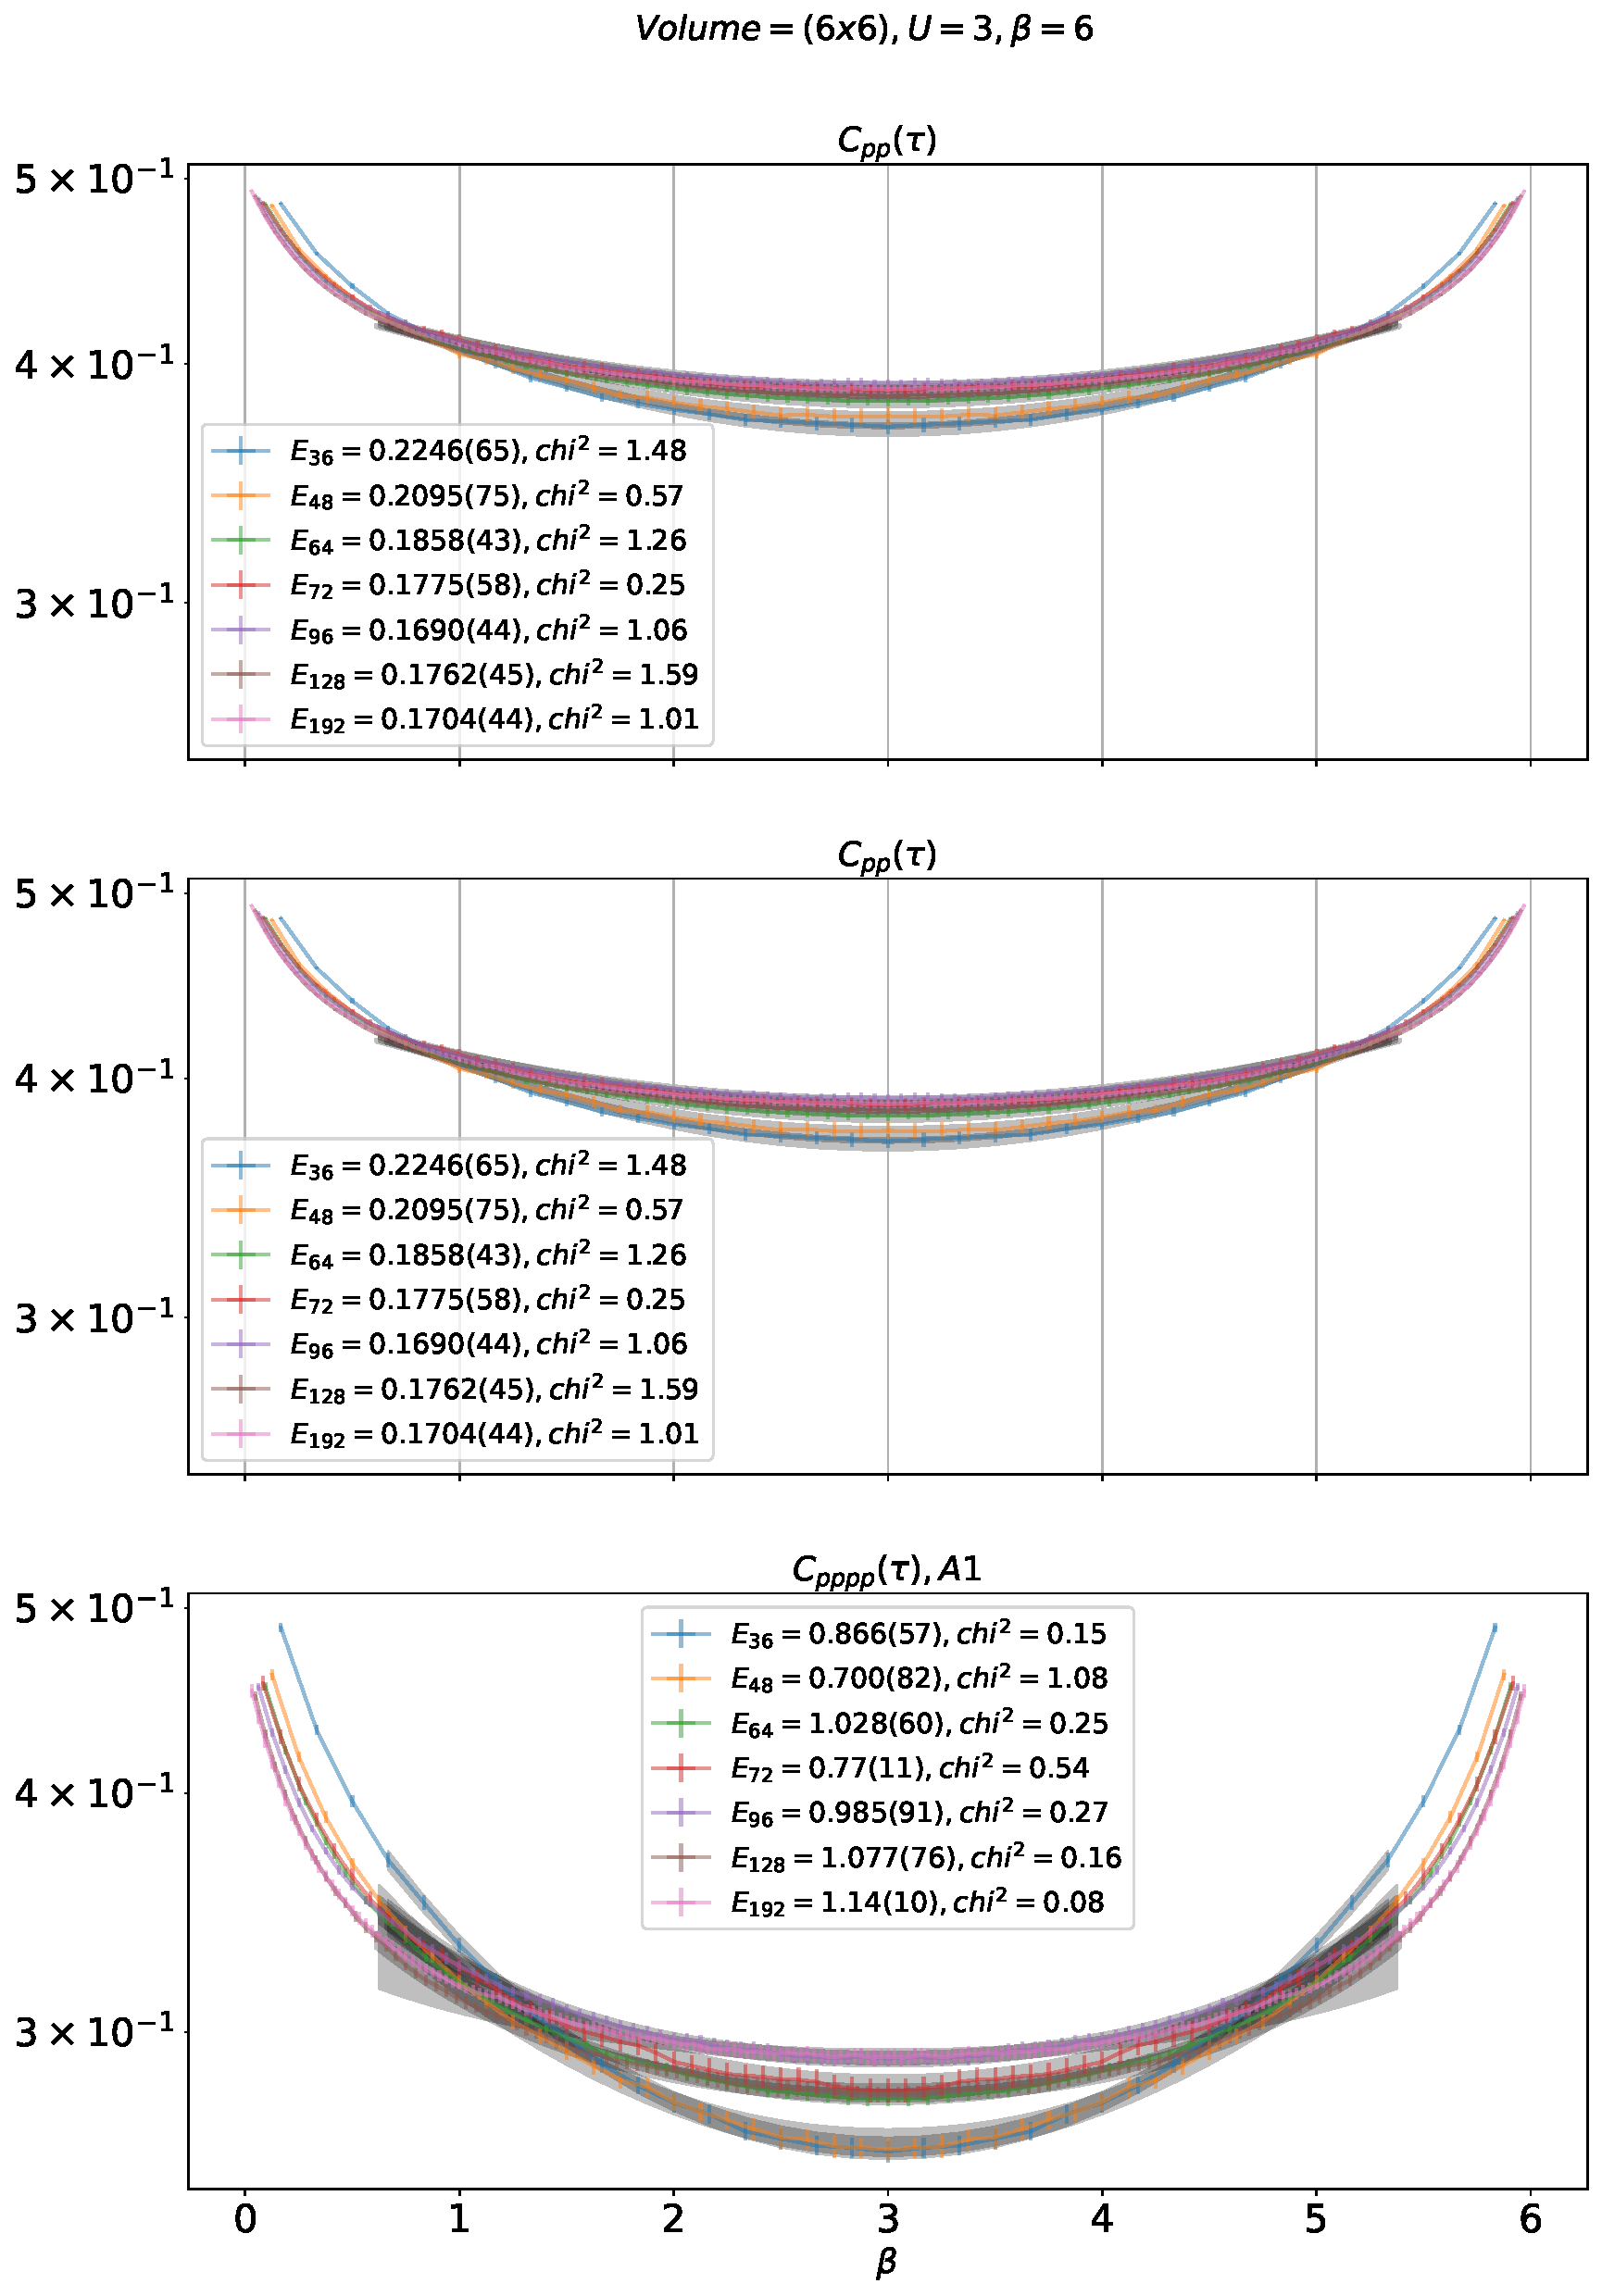
\includegraphics[width=\linewidth]{pppp-0-A1_6x6_U3.0_B6.0.pdf}
  \end{subfigure}%
  \begin{subfigure}{.5\textwidth}
    \centering
    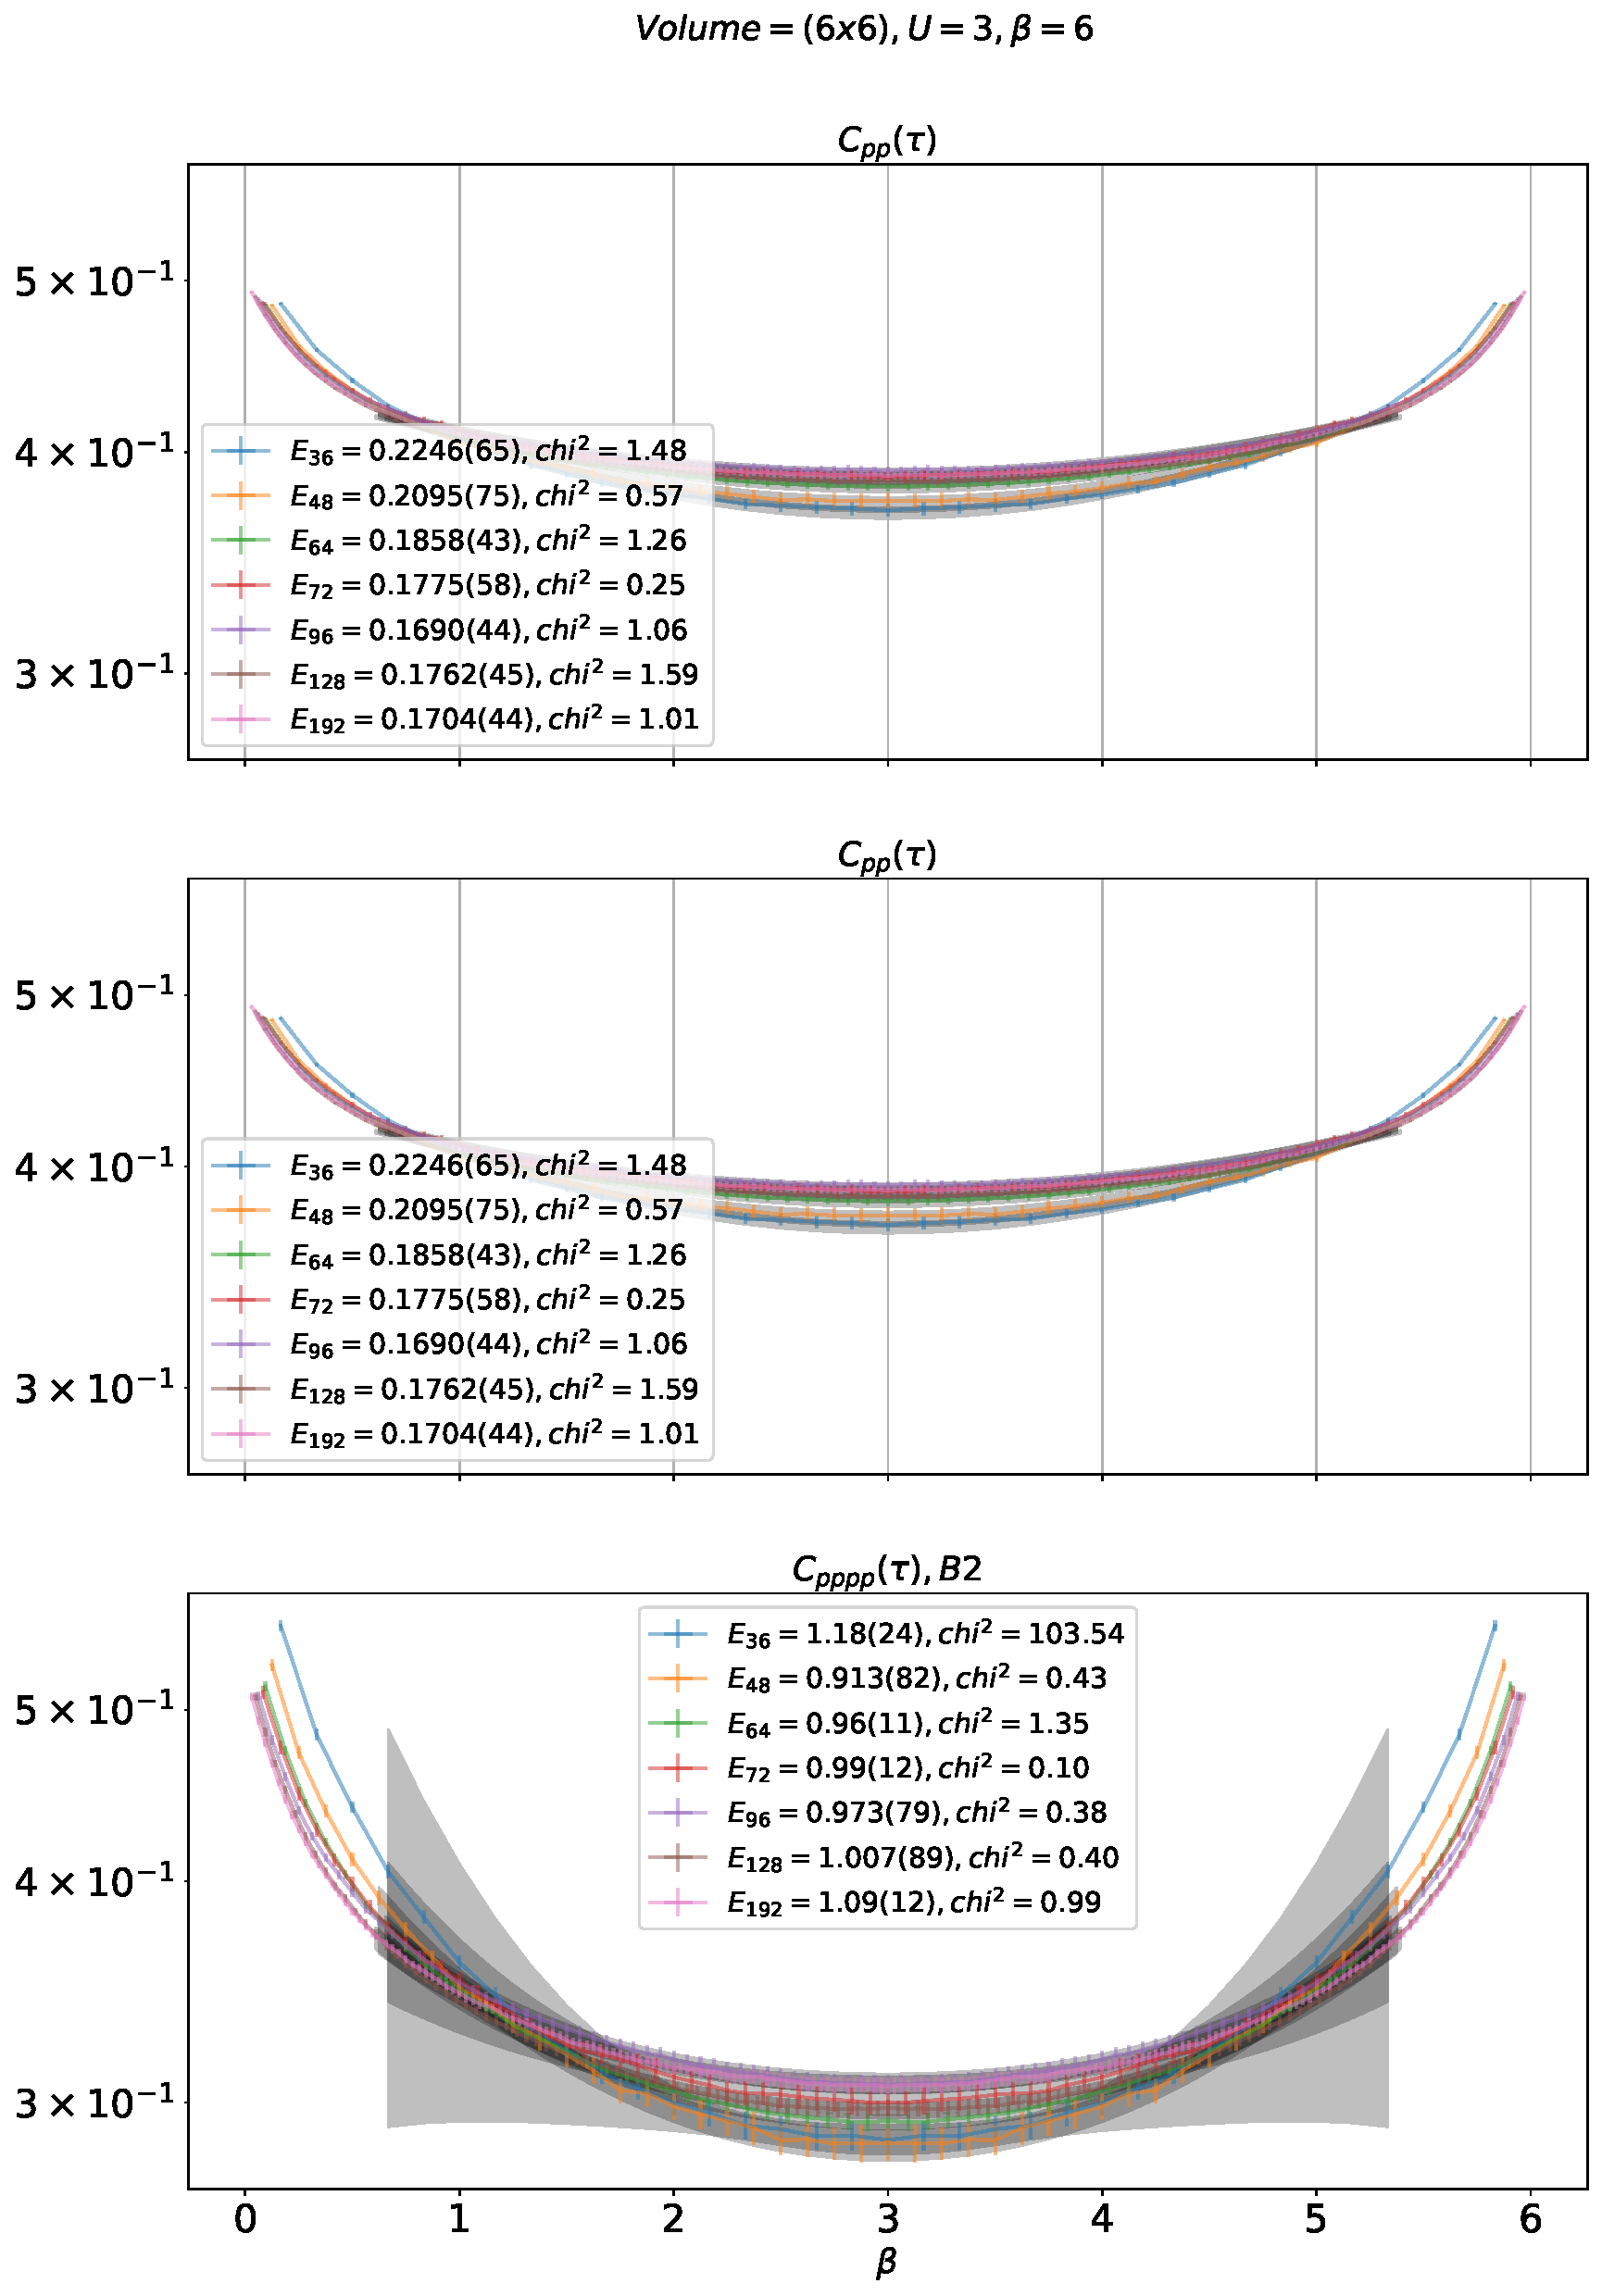
\includegraphics[width=\linewidth]{pppp-0-B2_6x6_U3.0_B6.0.pdf}
  \end{subfigure}
  \begin{subfigure}{.5\textwidth}
      \centering
      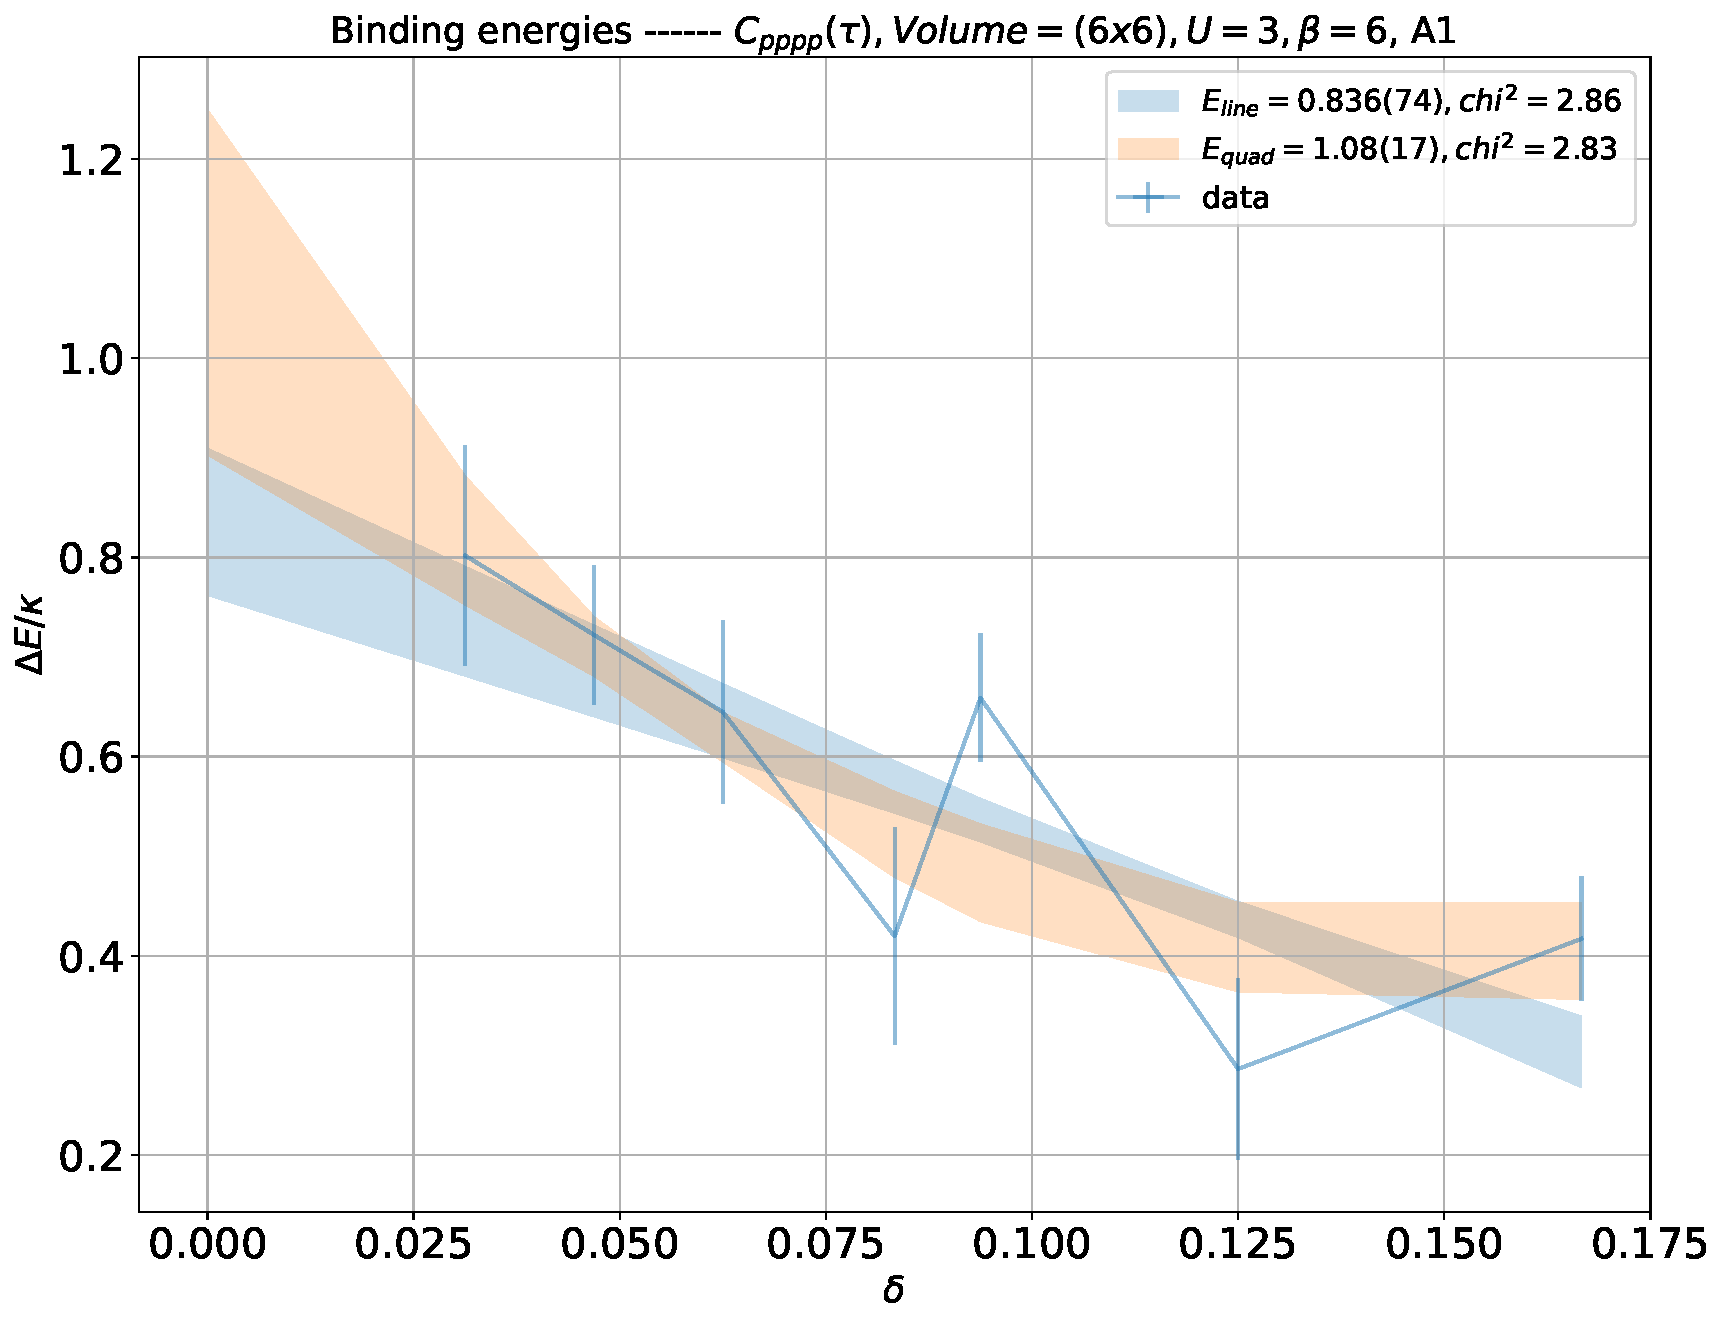
\includegraphics[width=\linewidth]{pppp-0-A1_6x6_U3.0_B6.0_cont.pdf}
  \end{subfigure}
  \begin{subfigure}{.5\textwidth}
      \centering
      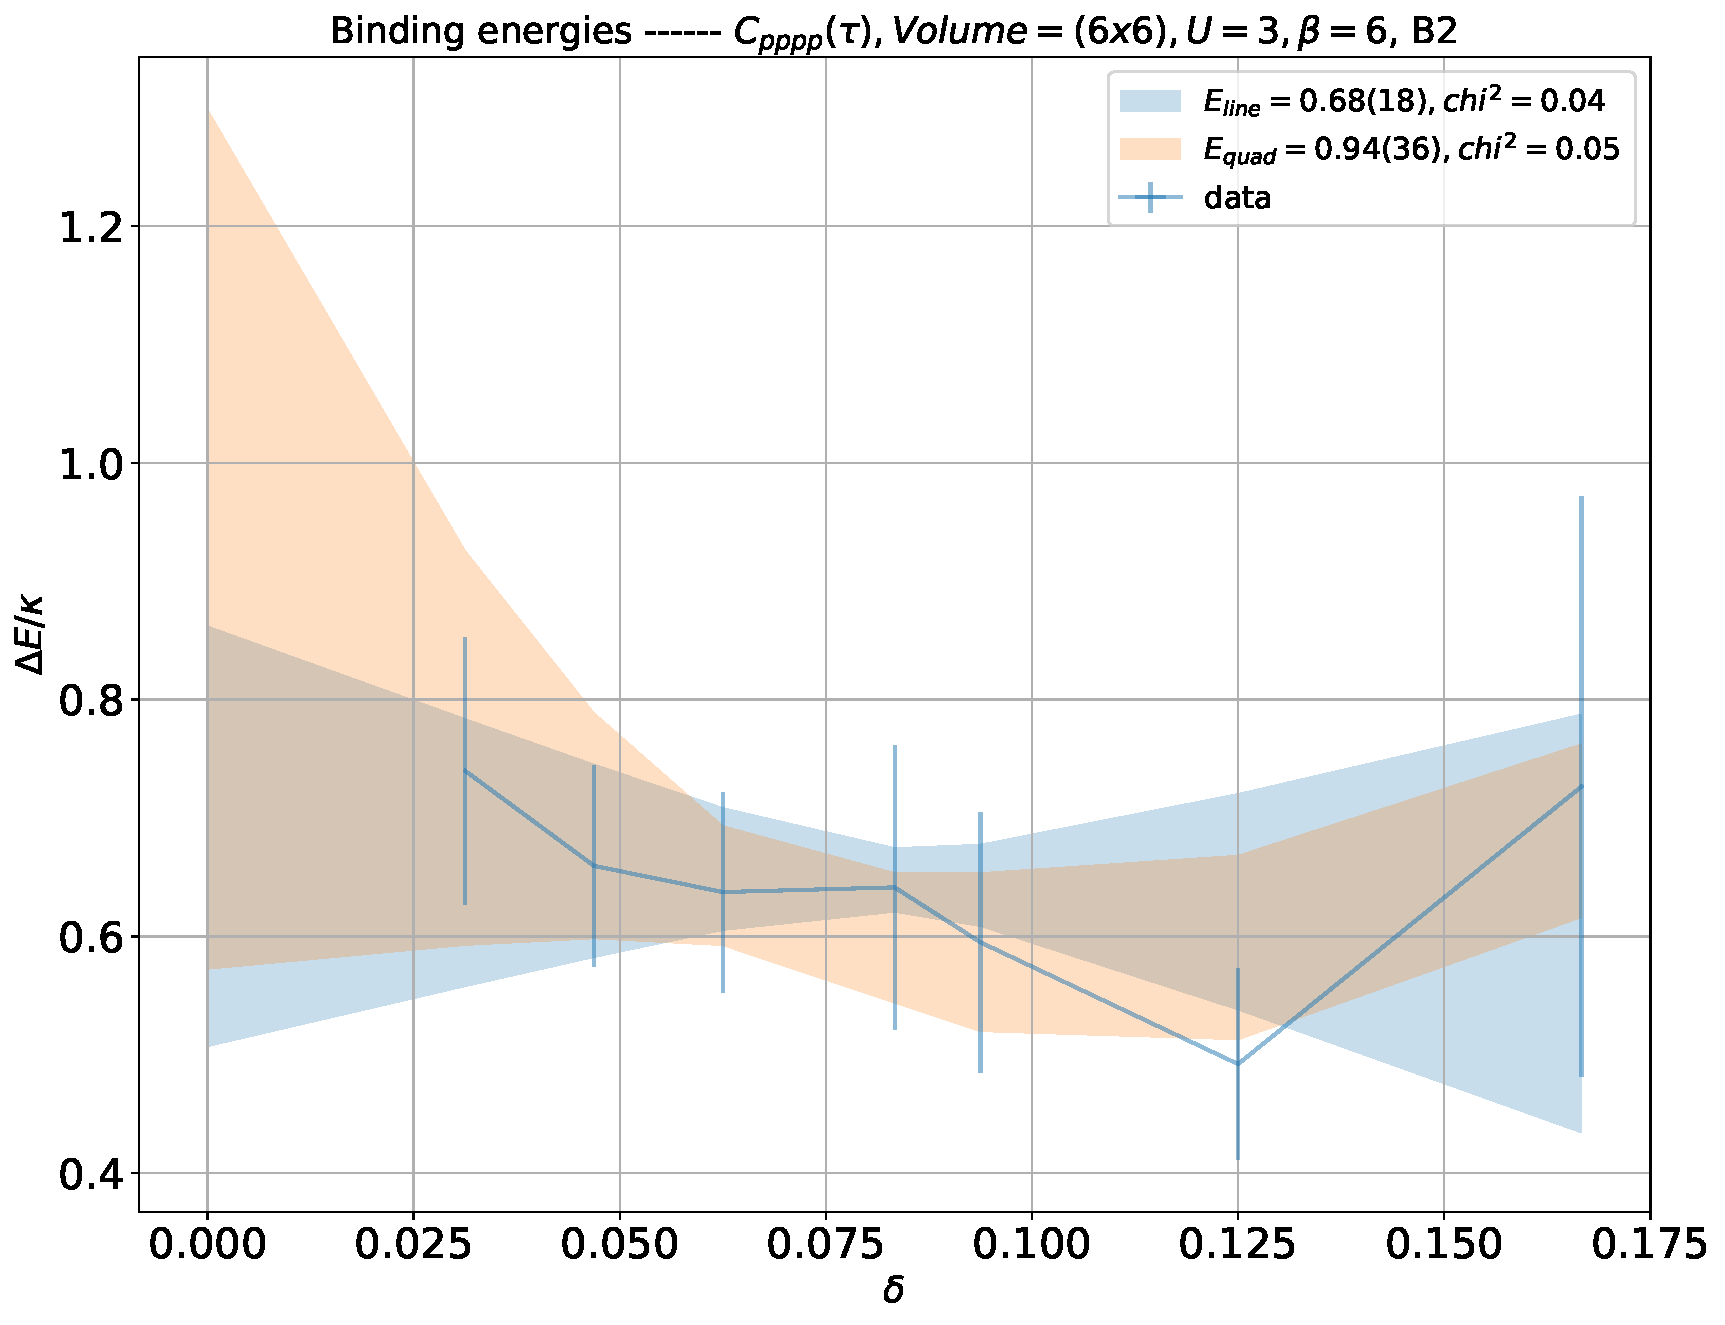
\includegraphics[width=\linewidth]{pppp-0-B2_6x6_U3.0_B6.0_cont.pdf}
  \end{subfigure}
  \caption{Binding energy extraction of the particle-particle pair at both irreducible representations, where we fit one- and two-body correlators for every $N_t$. This is followed by fitting a linear and a quadratic functions to the $\Delta E_{N_t}$ in order to extrapolate to the continuum limit ($N_t\to\infty$).}
  \label{fig:fig6}
\end{figure}

\begin{figure}
  \begin{subfigure}{.5\textwidth}
    \centering
    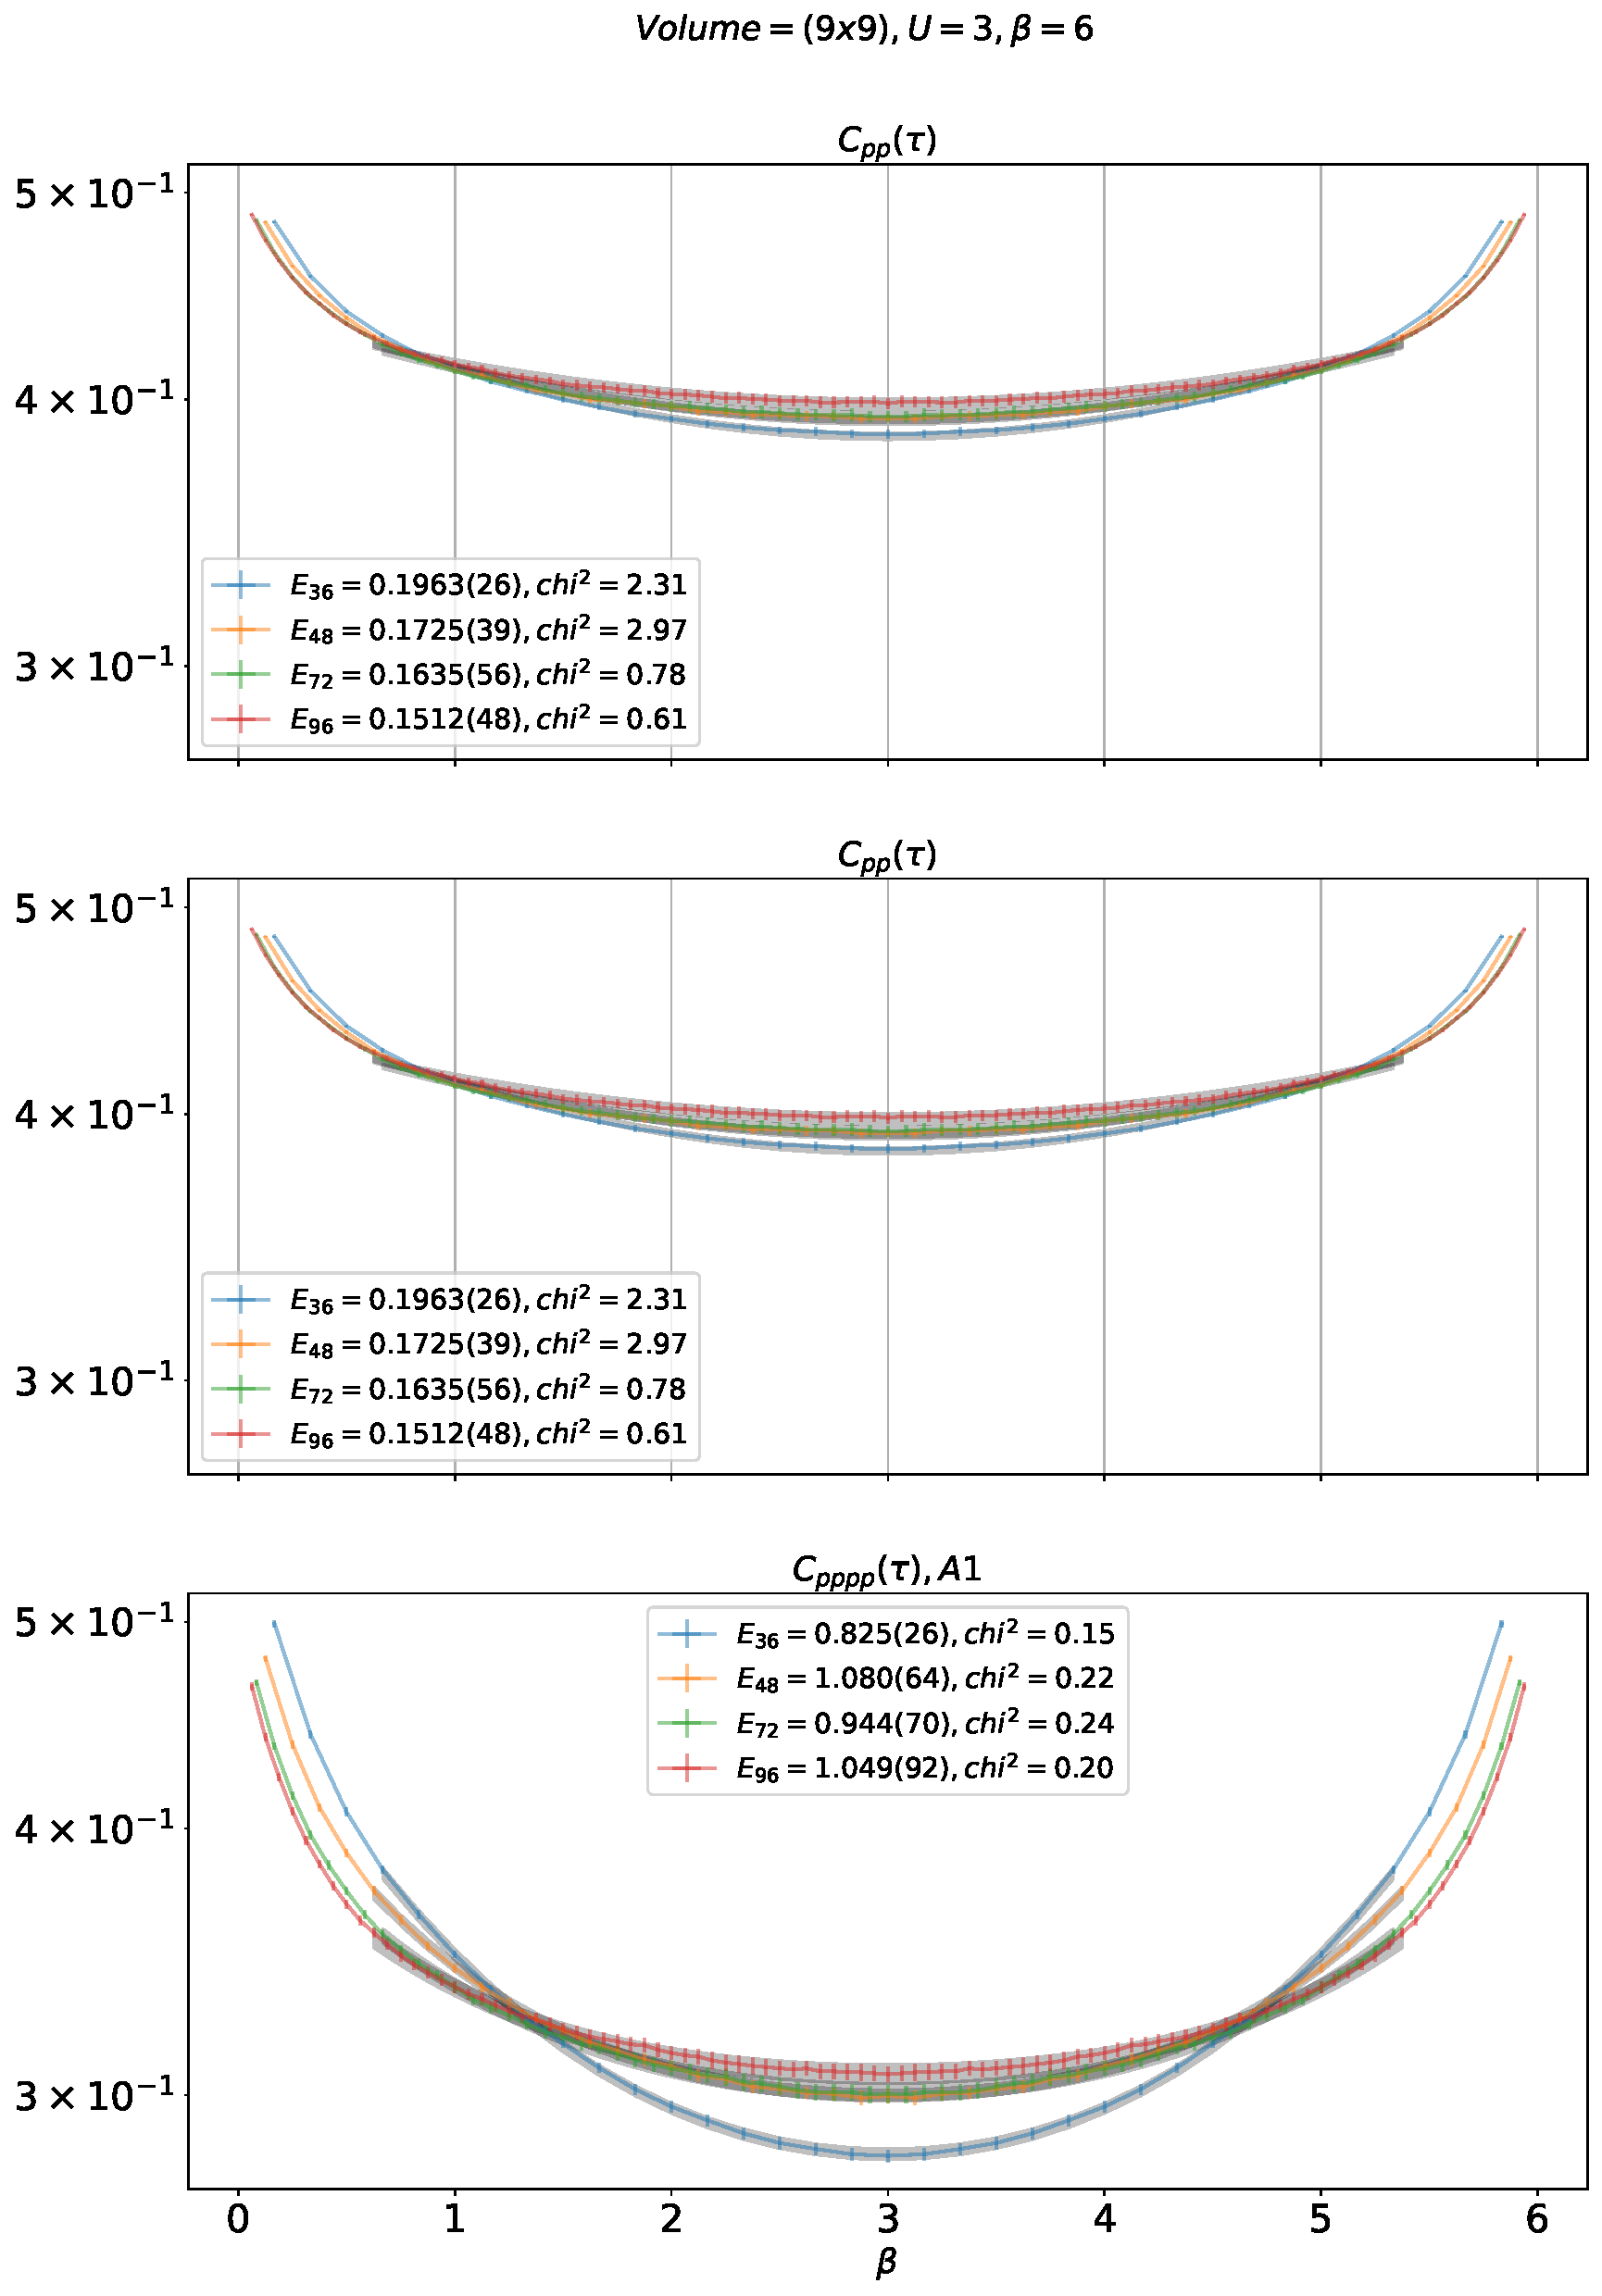
\includegraphics[width=\linewidth]{pppp-0-A1_9x9_U3_B6.pdf}
  \end{subfigure}%
  \begin{subfigure}{.5\textwidth}
    \centering
    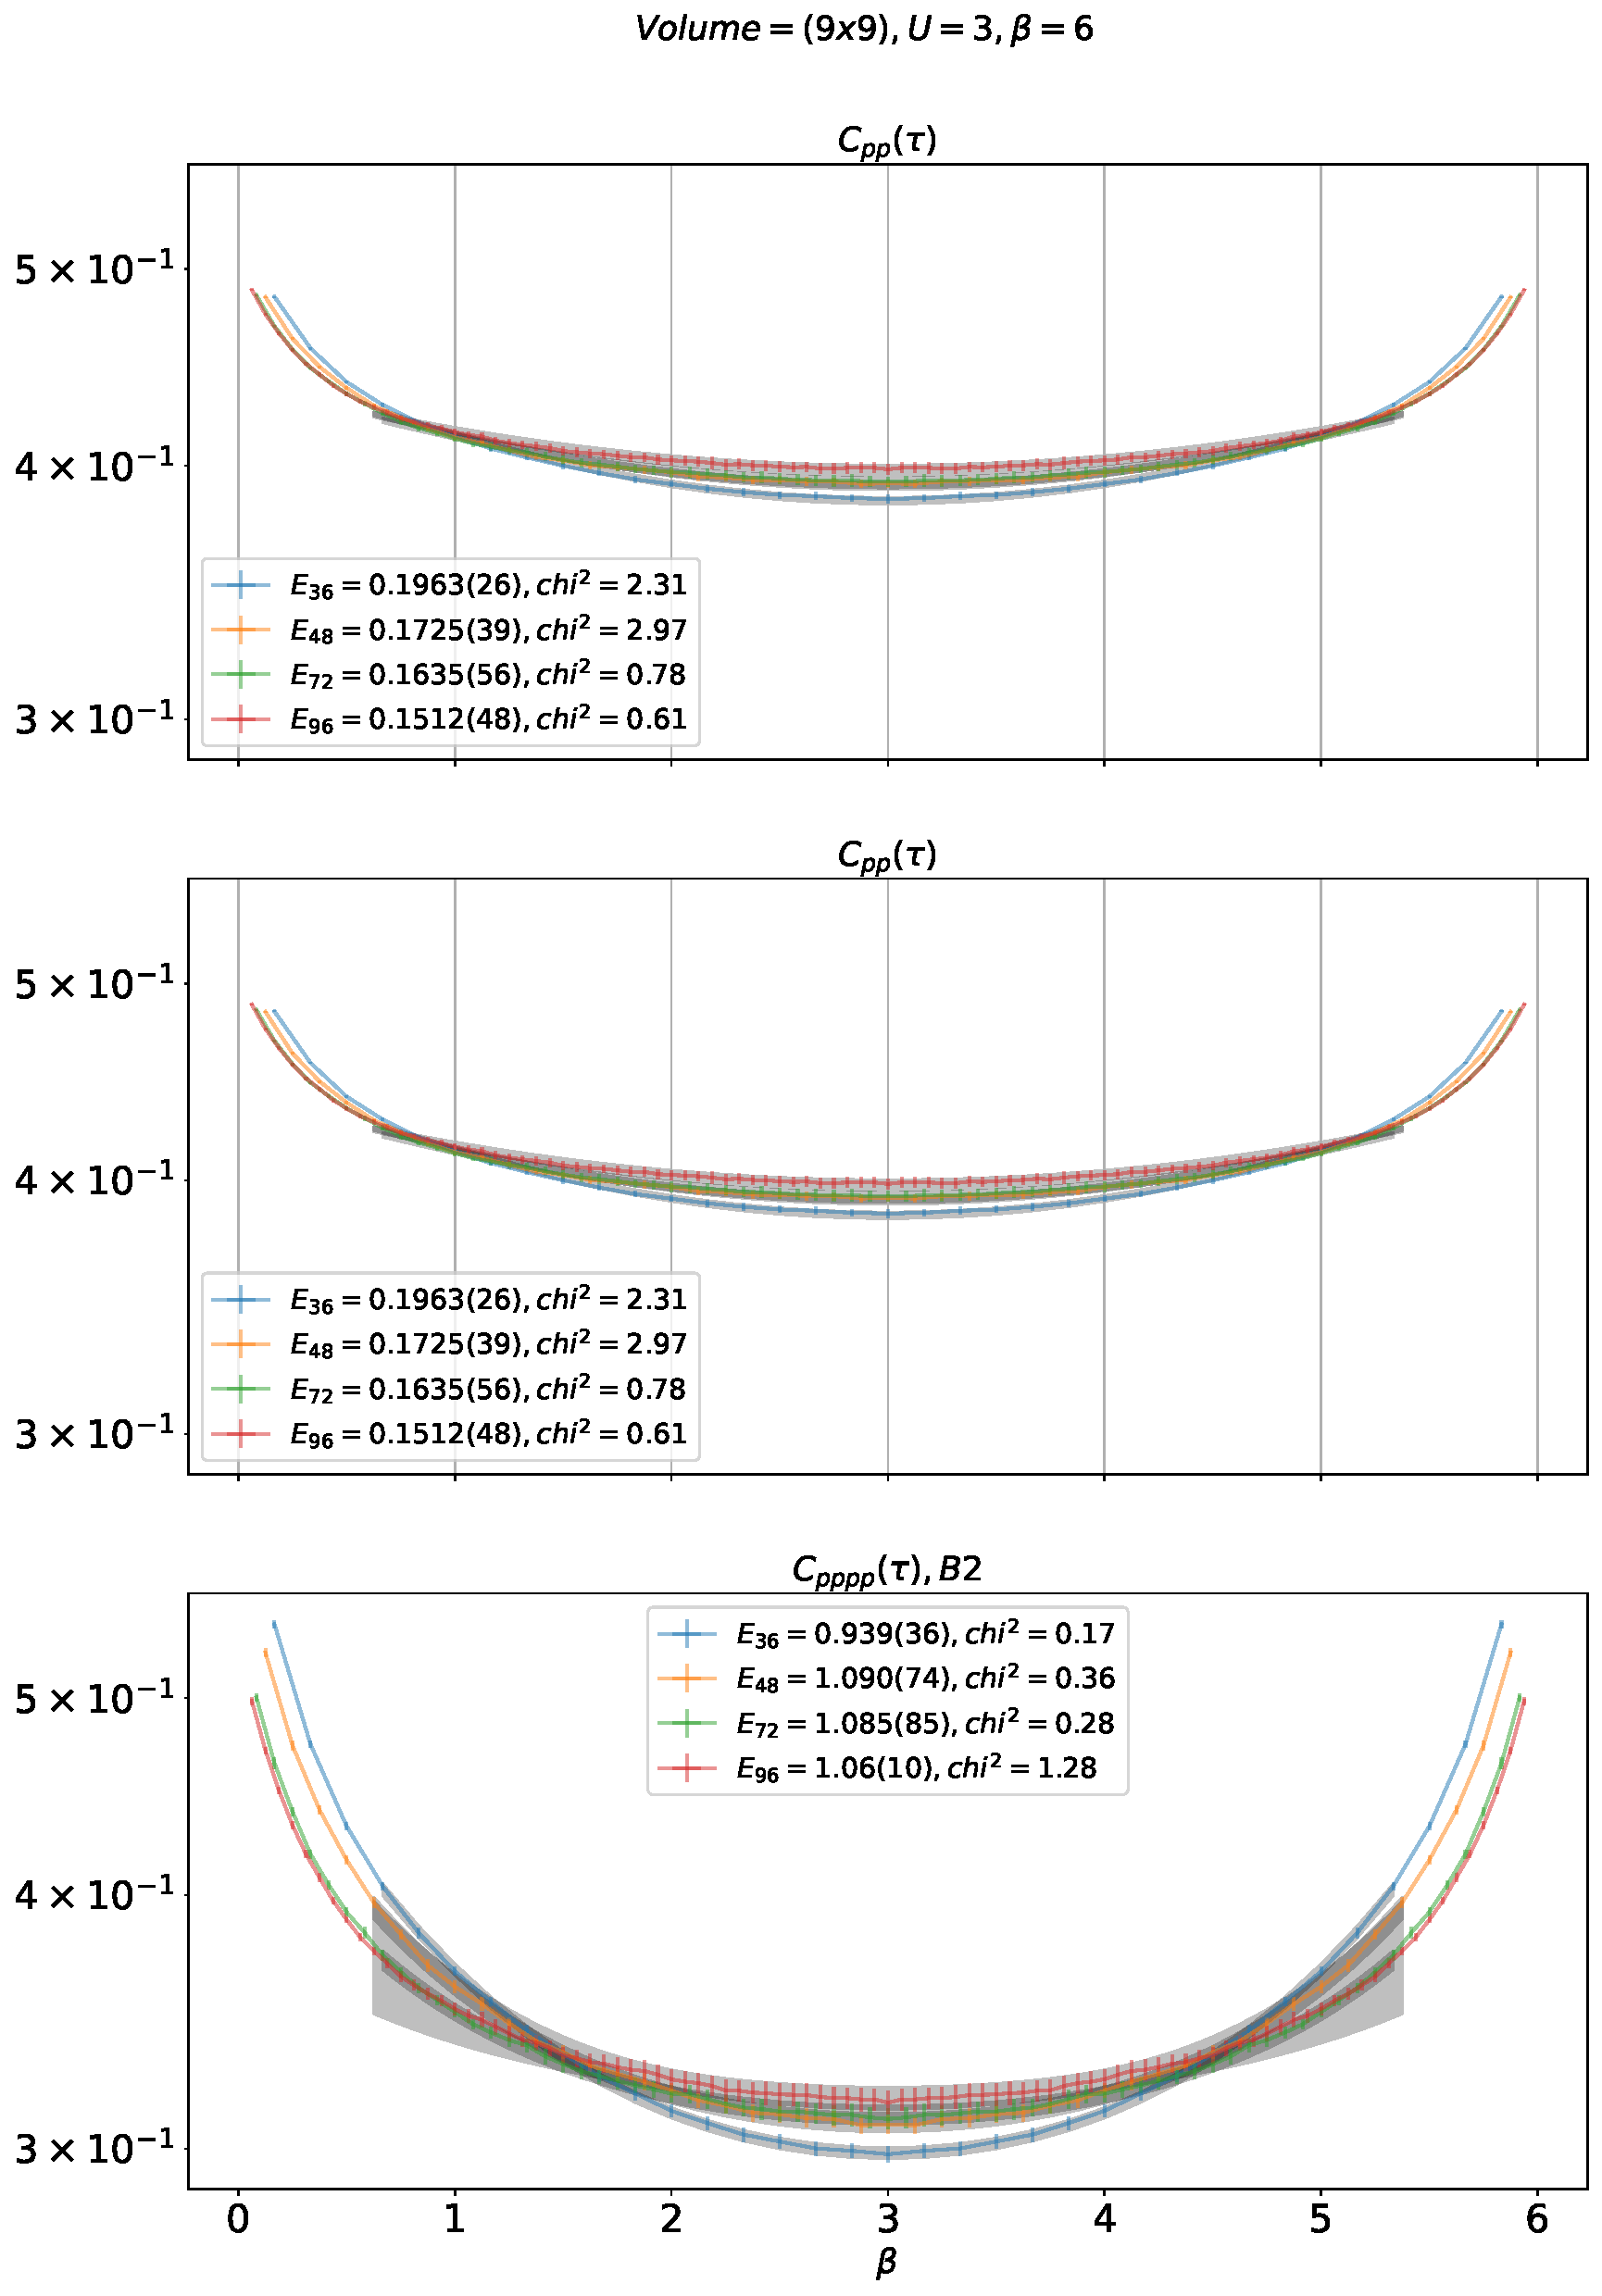
\includegraphics[width=\linewidth]{pppp-0-B2_9x9_U3_B6.pdf}
  \end{subfigure}
  \begin{subfigure}{.5\textwidth}
      \centering
      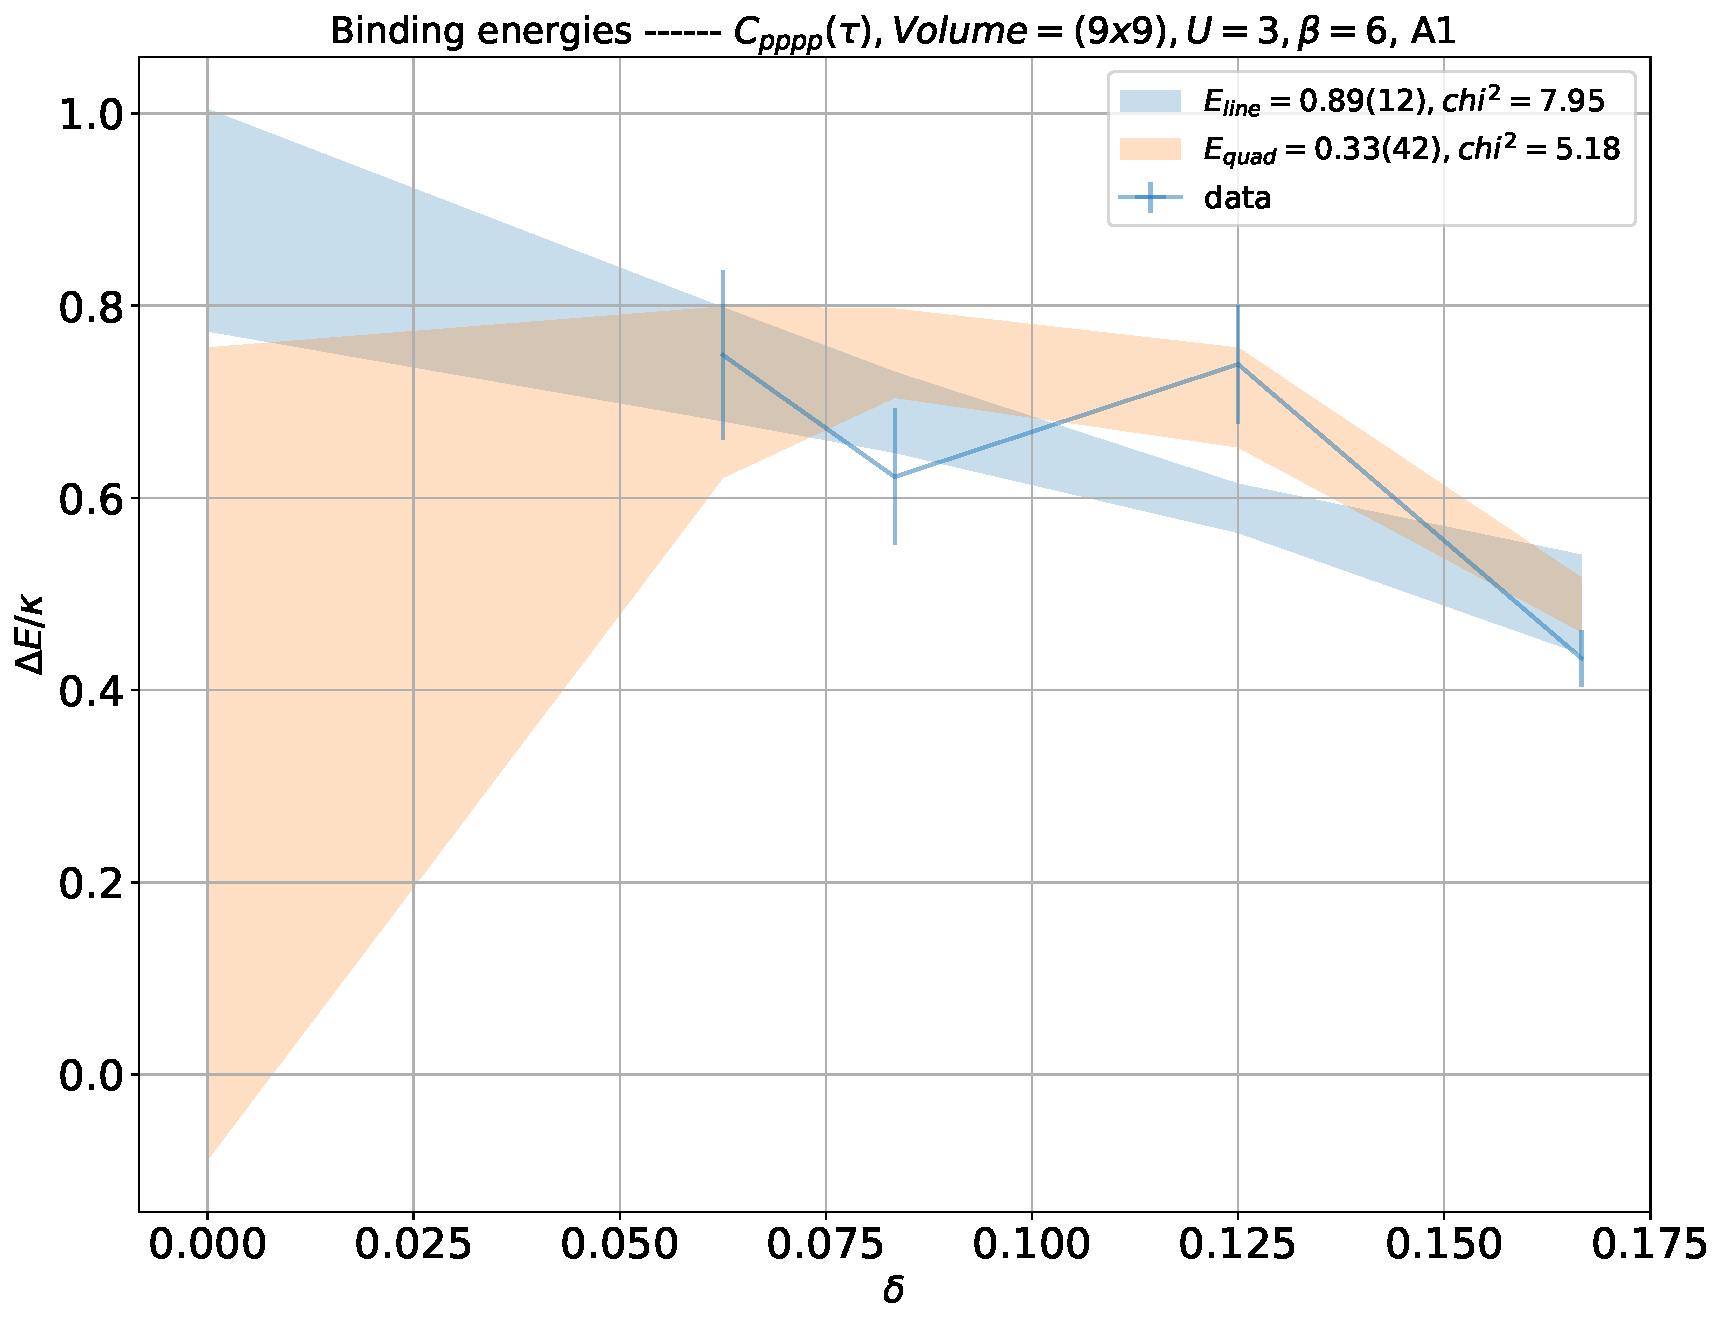
\includegraphics[width=\linewidth]{pppp-0-A1_9x9_U3_B6_cont.pdf}
  \end{subfigure}
  \begin{subfigure}{.5\textwidth}
      \centering
      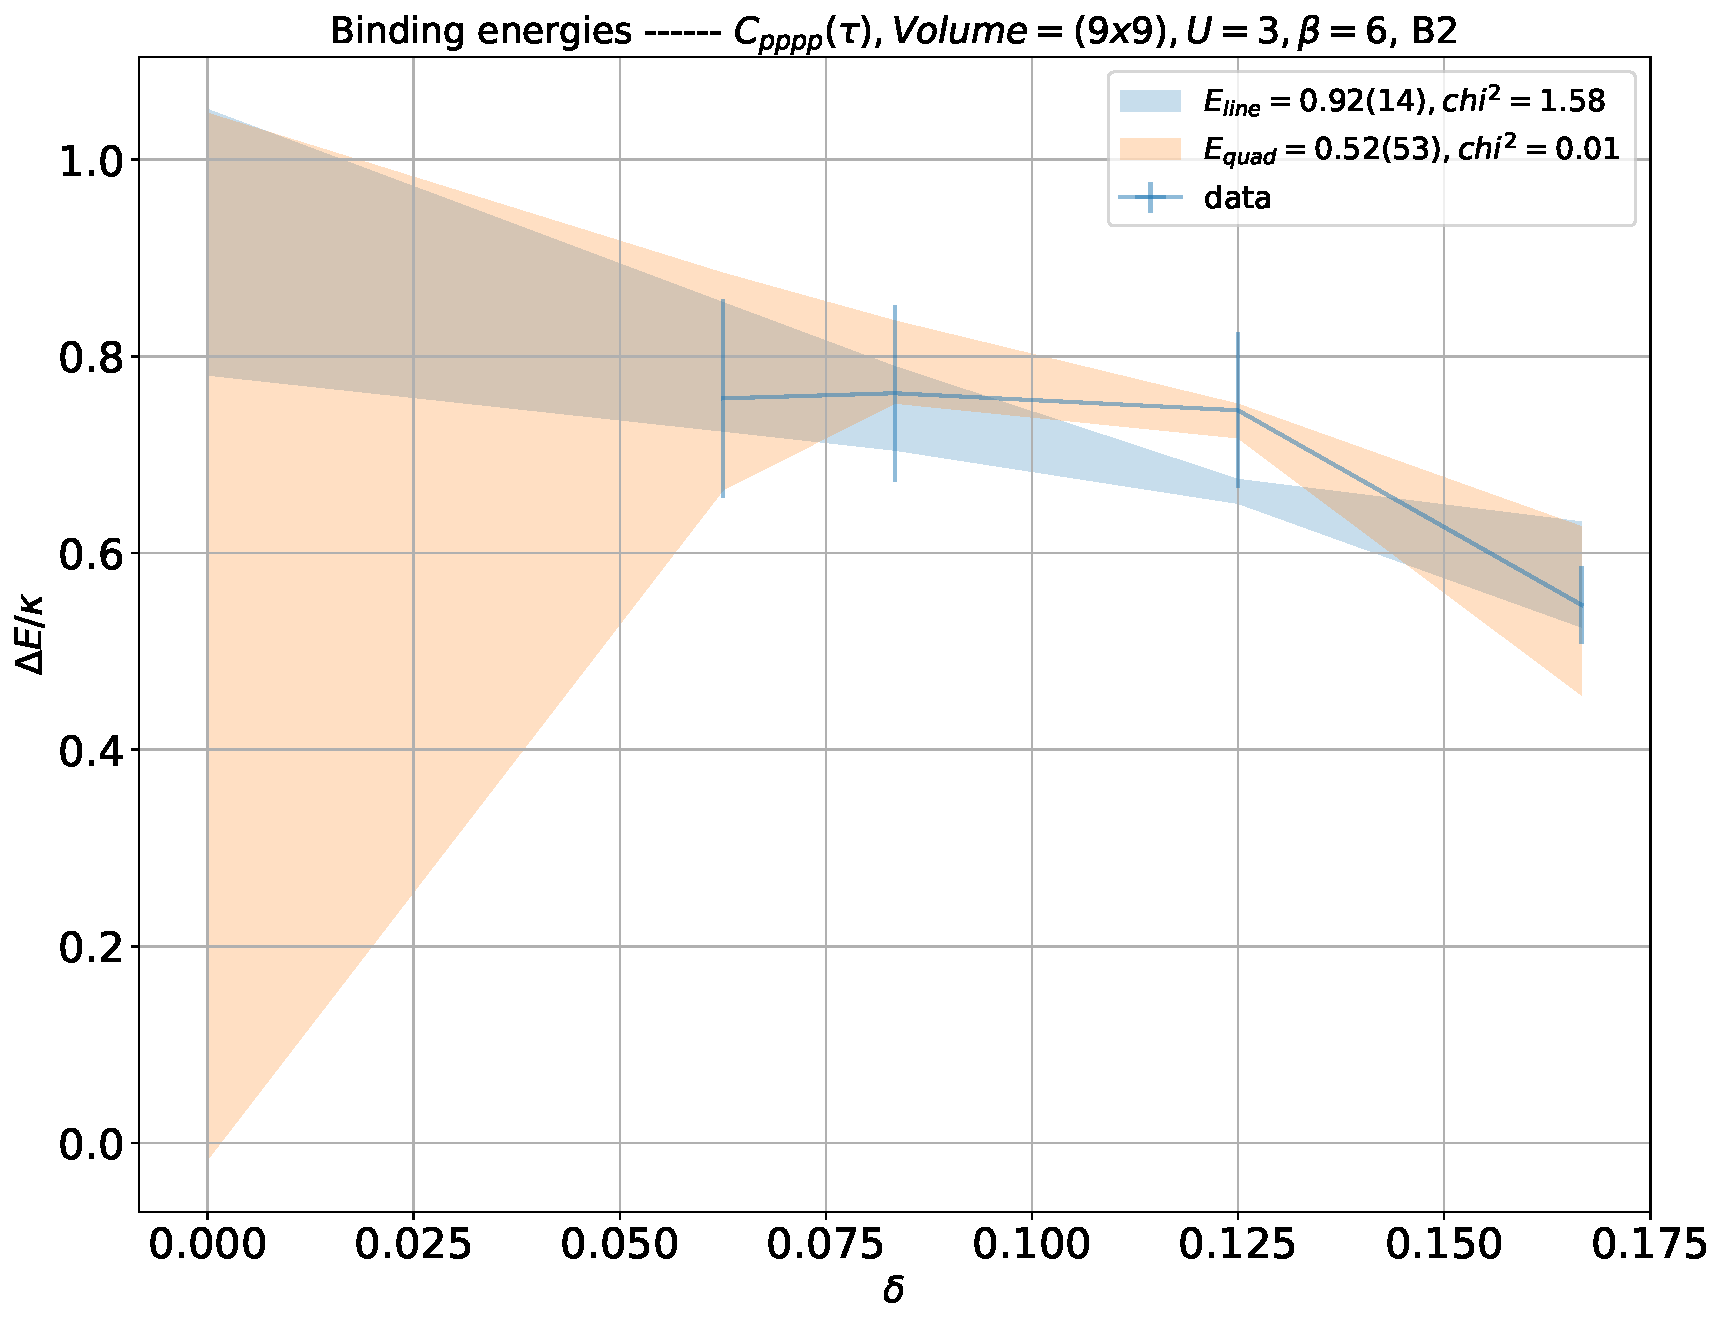
\includegraphics[width=\linewidth]{pppp-0-B2_9x9_U3_B6_cont.pdf}
  \end{subfigure}
  \caption{Binding energy extraction of the particle-particle pair at both irreducible representations, where we fit one- and two-body correlators for every $N_t$. This is followed by fitting a linear and a quadratic functions to the $\Delta E_{N_t}$ in order to extrapolate to the continuum limit ($N_t\to\infty$).}
  \label{fig:fig7}
\end{figure}

\begin{figure}
  \begin{subfigure}{.5\textwidth}
    \centering
    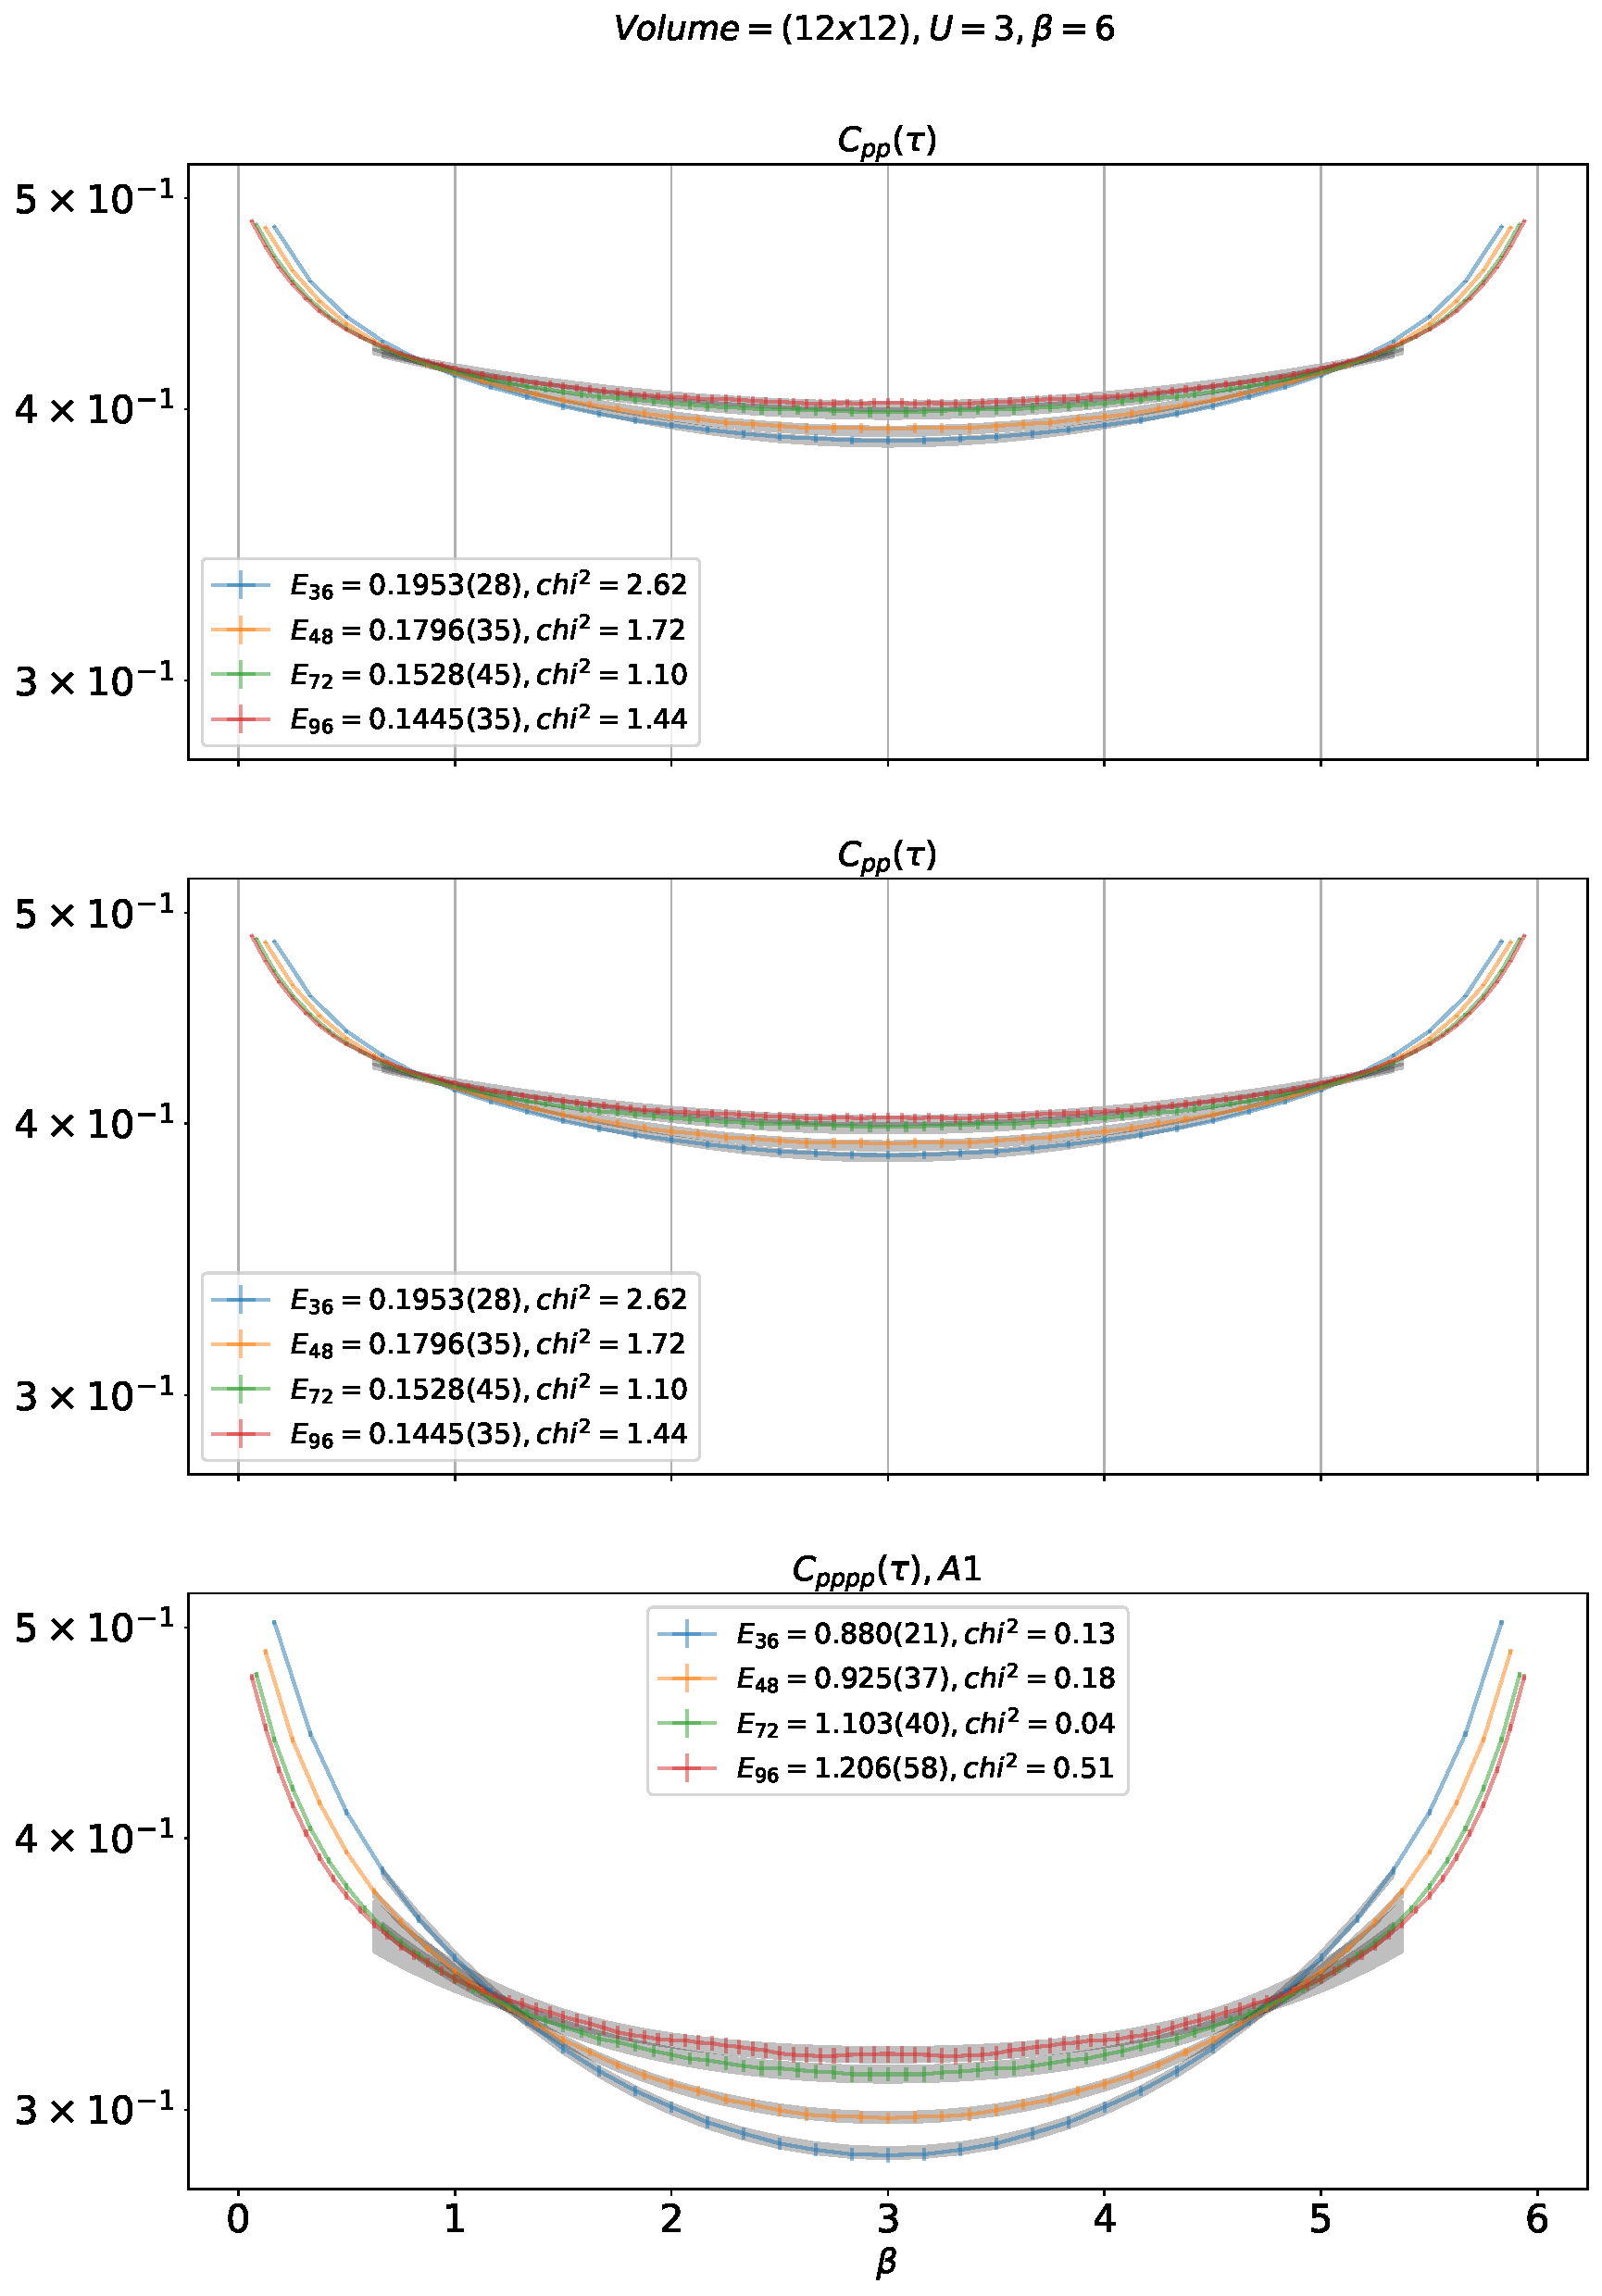
\includegraphics[width=\linewidth]{pppp-0-A1_12x12_U3_B6.pdf}
  \end{subfigure}%
  \begin{subfigure}{.5\textwidth}
    \centering
    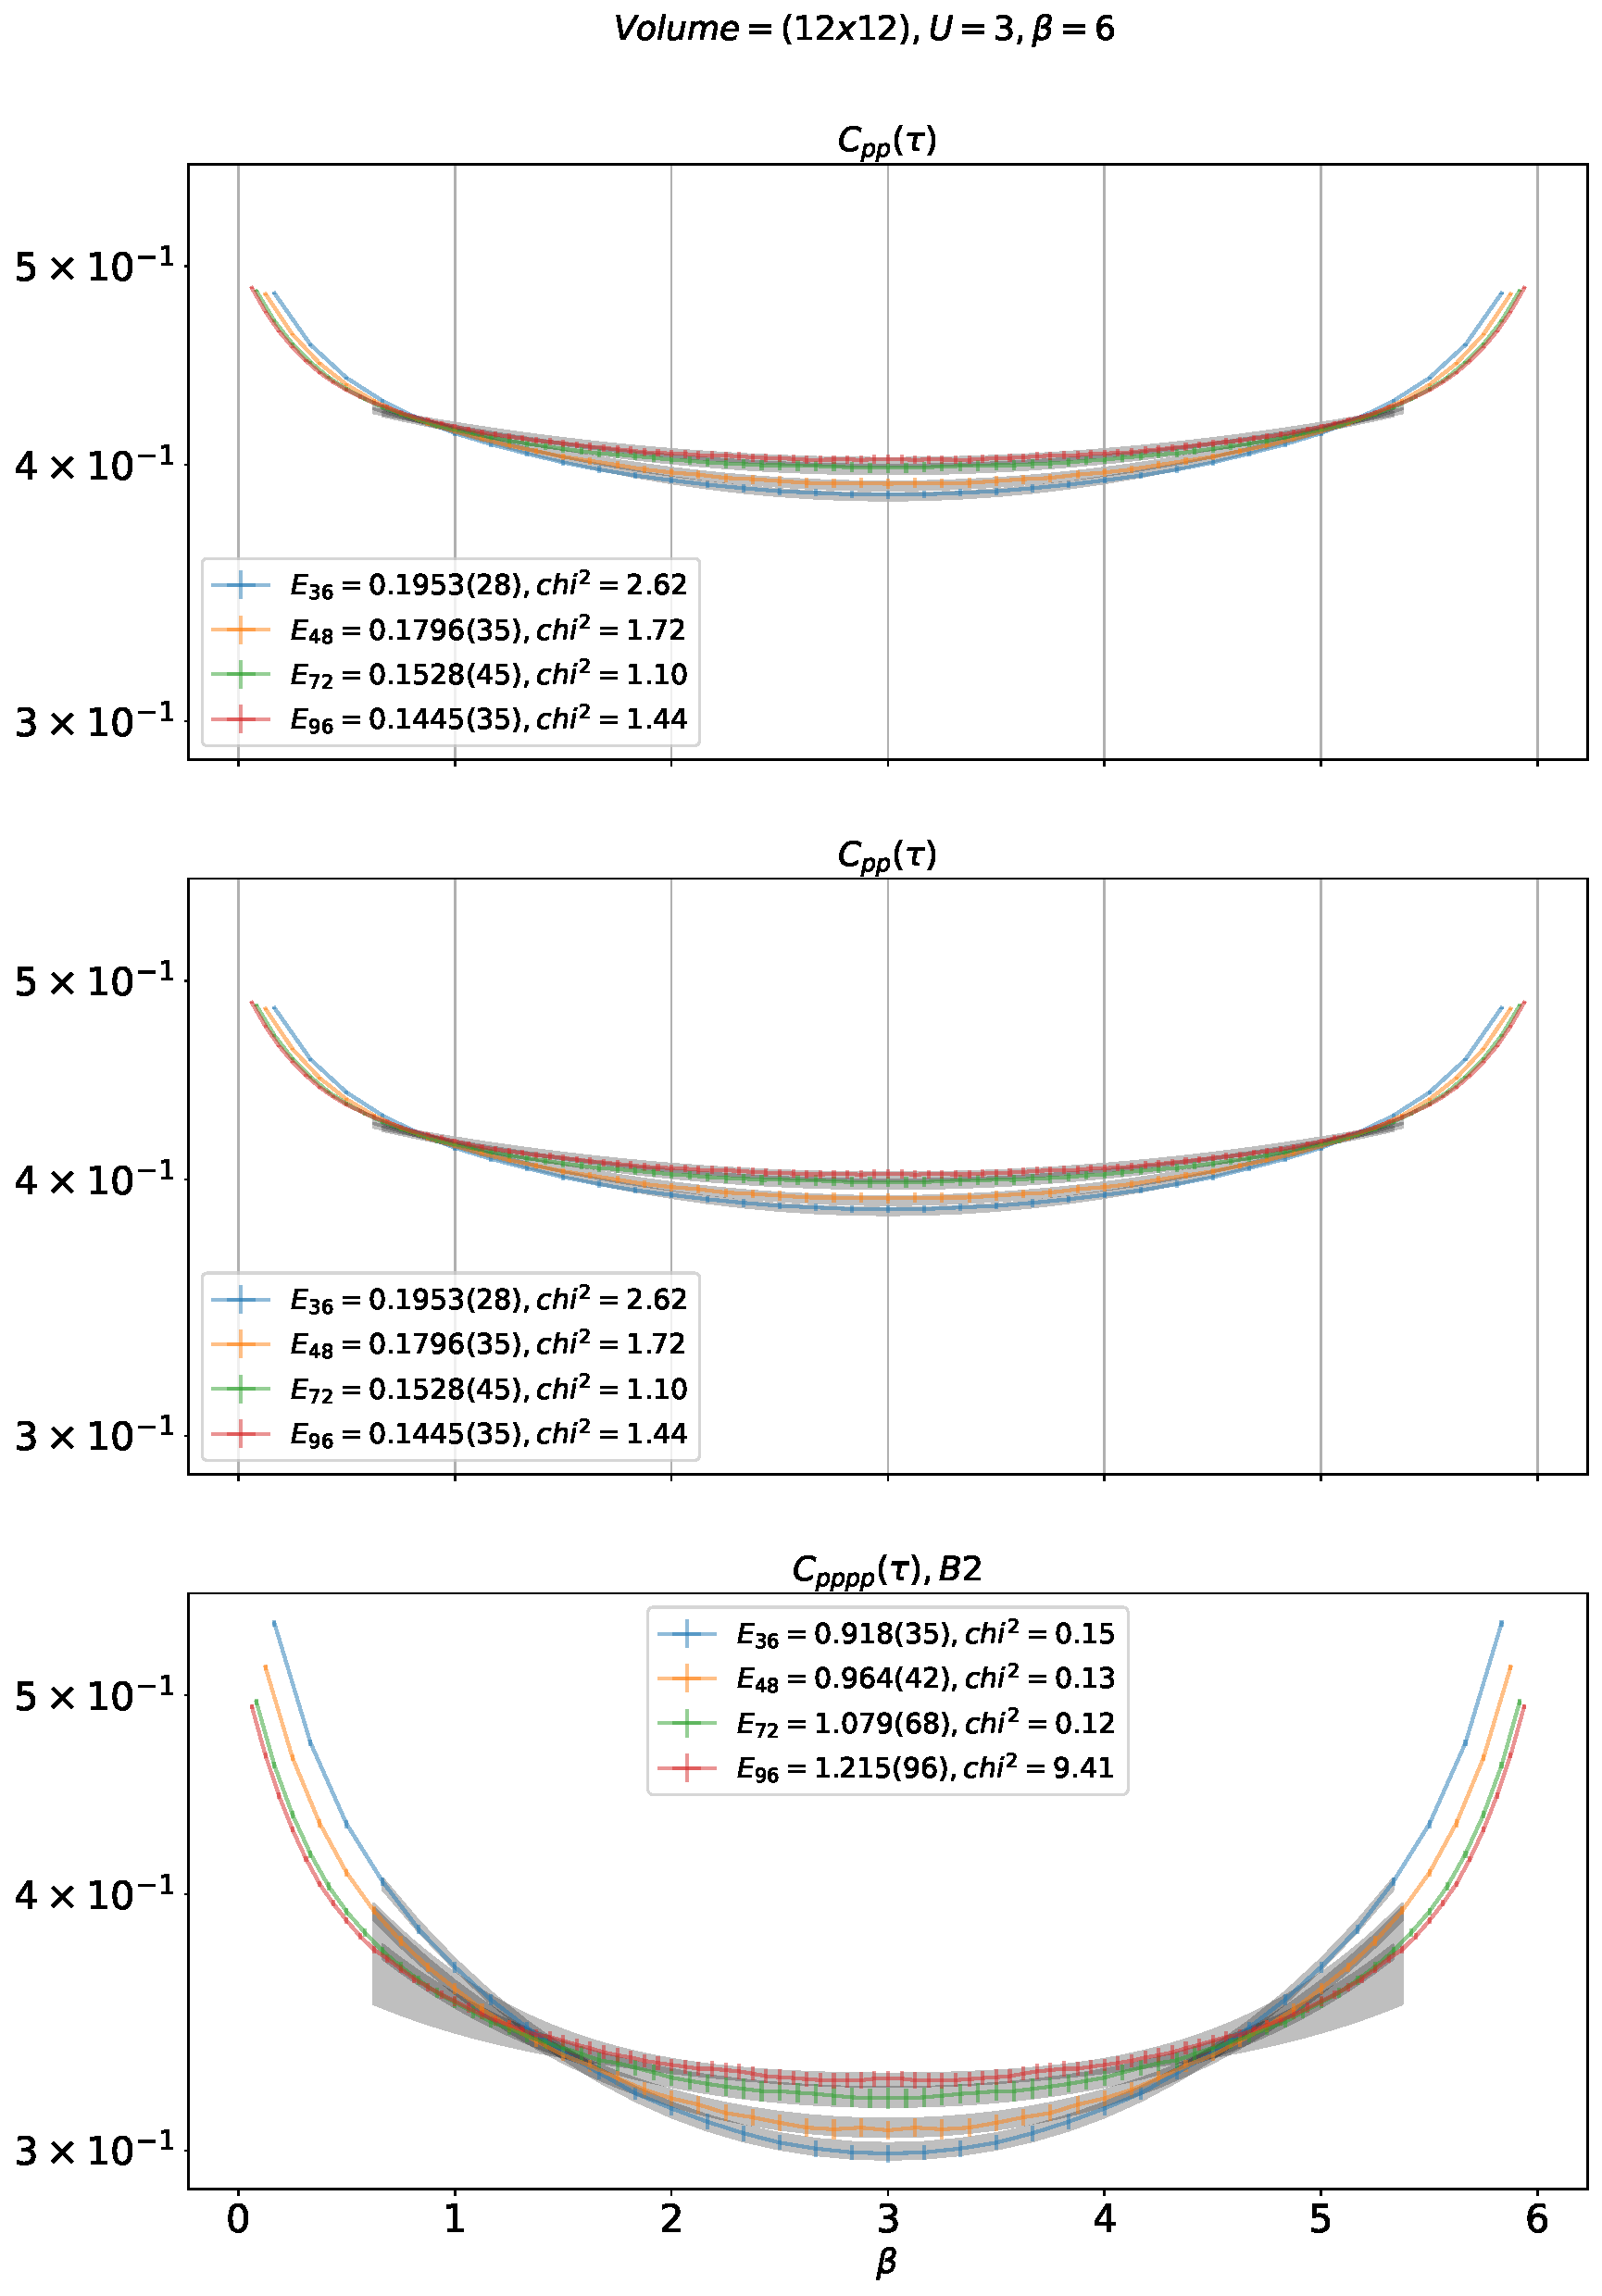
\includegraphics[width=\linewidth]{pppp-0-B2_12x12_U3_B6.pdf}
  \end{subfigure}
  \begin{subfigure}{.5\textwidth}
      \centering
      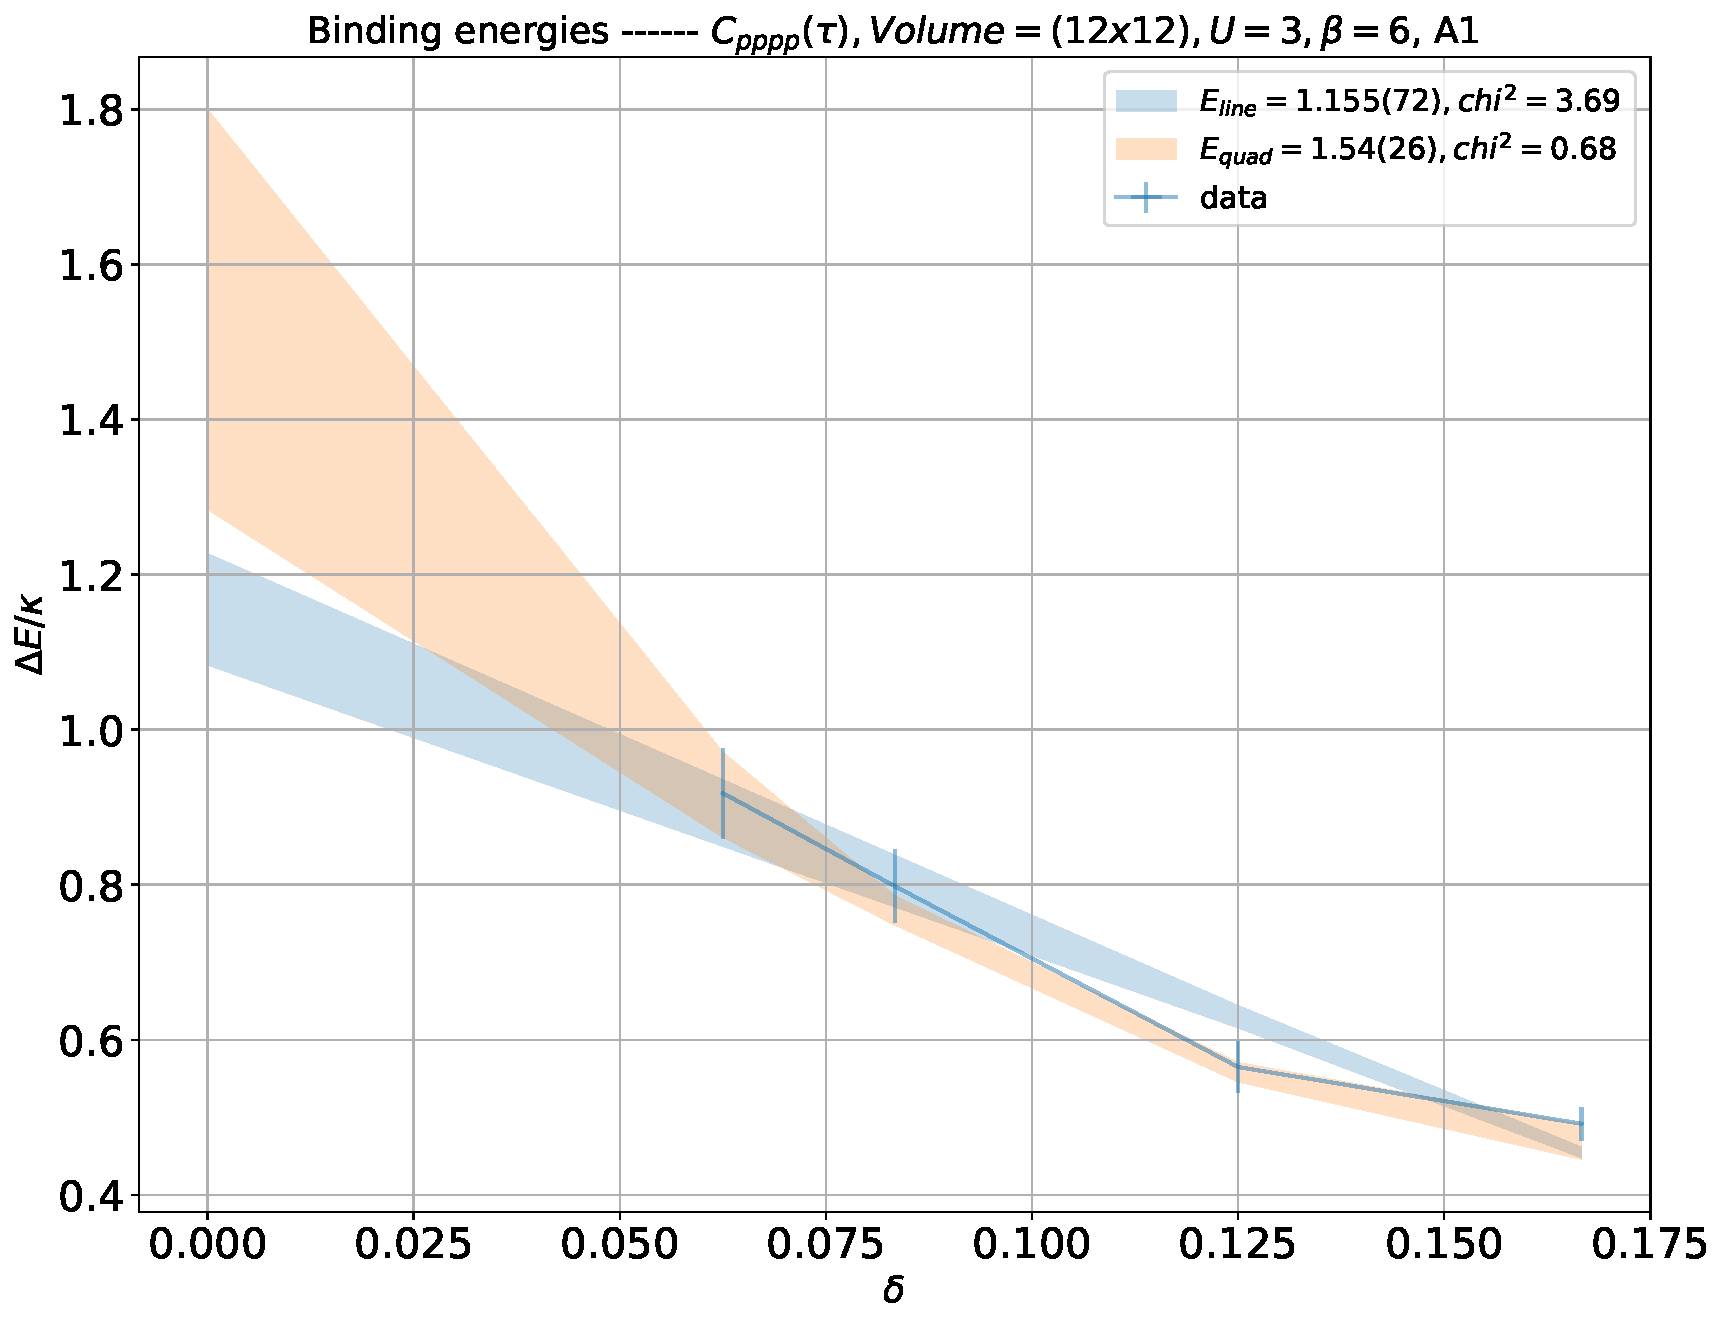
\includegraphics[width=\linewidth]{pppp-0-A1_12x12_U3_B6_cont.pdf}
  \end{subfigure}
  \begin{subfigure}{.5\textwidth}
      \centering
      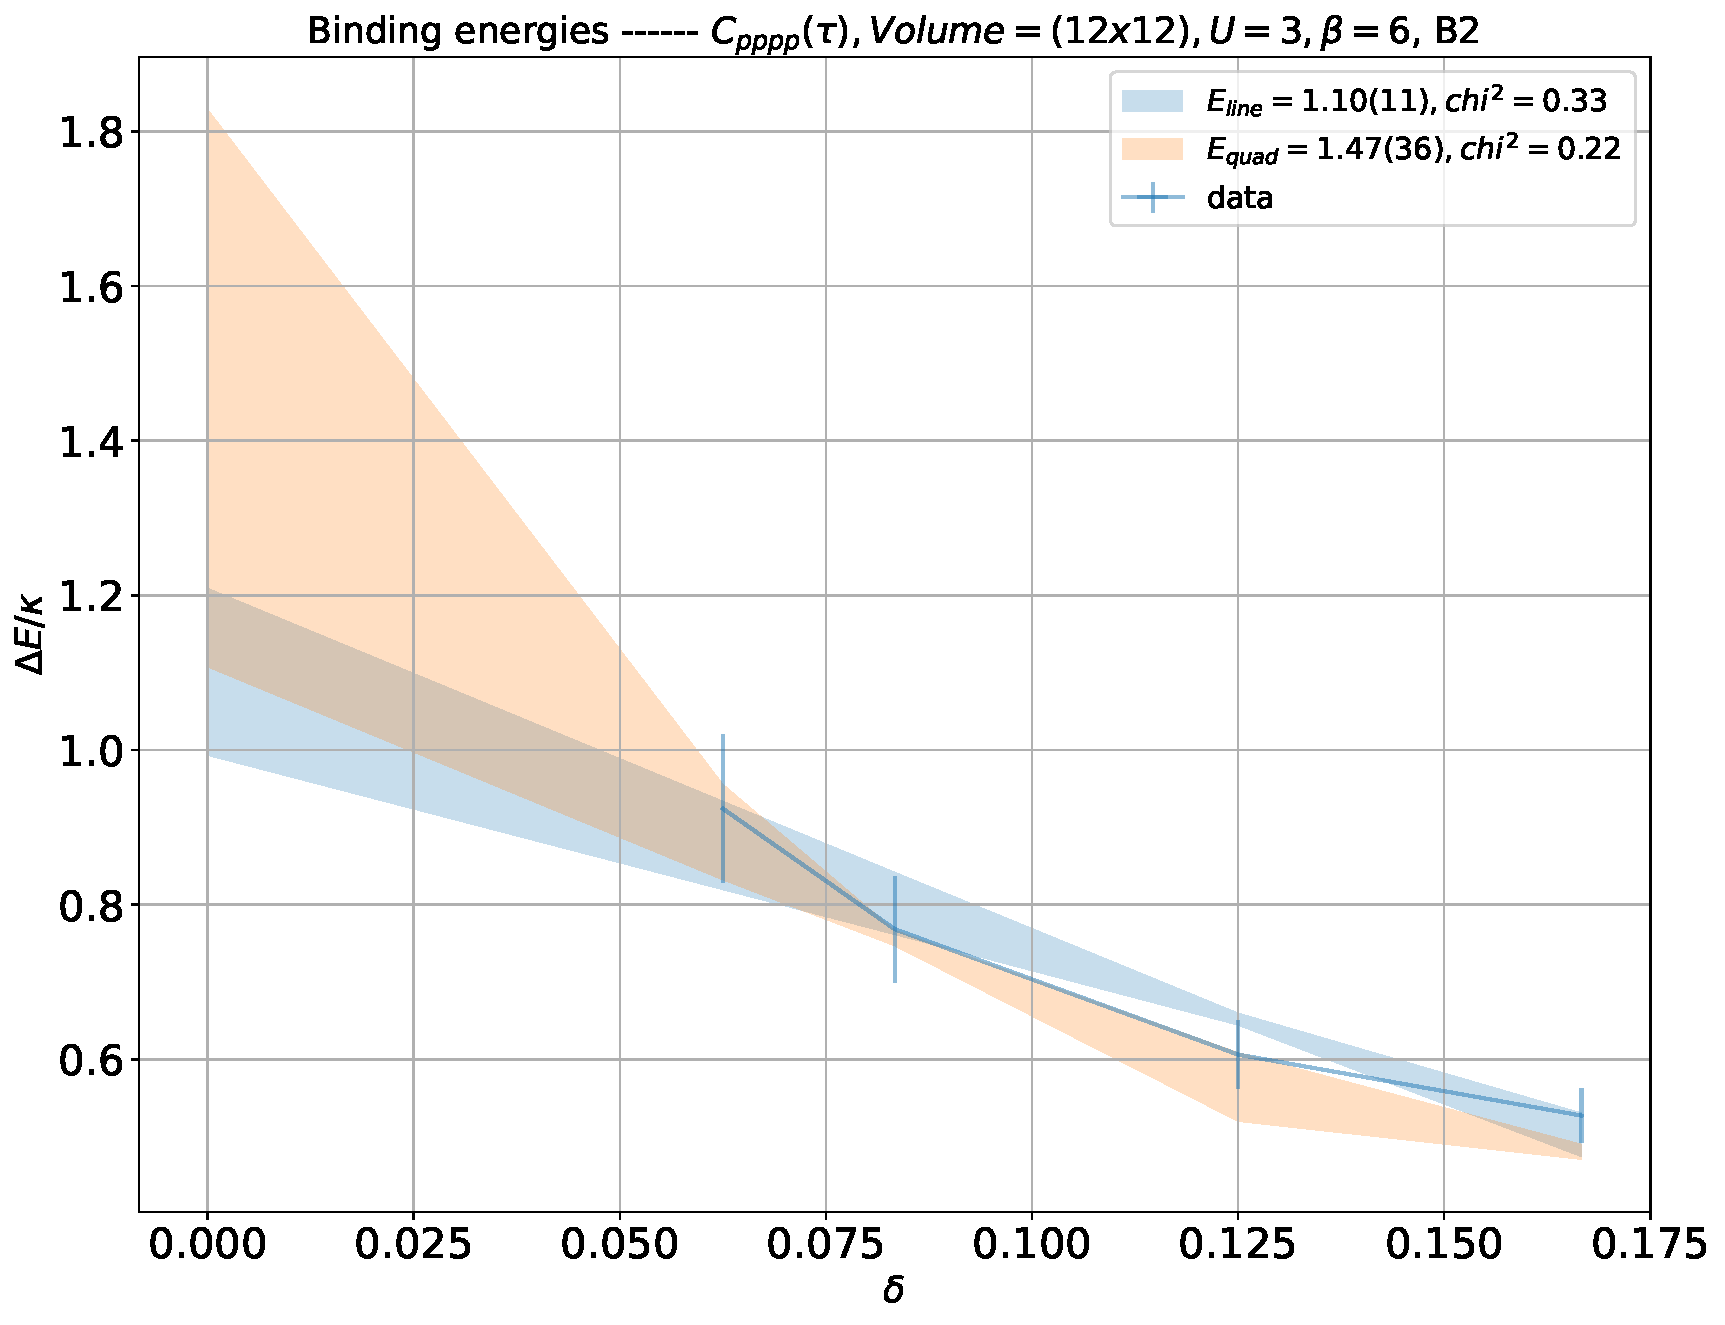
\includegraphics[width=\linewidth]{pppp-0-B2_12x12_U3_B6_cont.pdf}
  \end{subfigure}
  \caption{Binding energy extraction of the particle-particle pair at both irreducible representations, where we fit one- and two-body correlators for every $N_t$. This is followed by fitting a linear and a quadratic functions to the $\Delta E_{N_t}$ in order to extrapolate to the continuum limit ($N_t\to\infty$).}
  \label{fig:fig8}
\end{figure}

\begin{figure}
  \begin{subfigure}{.5\textwidth}
    \centering
    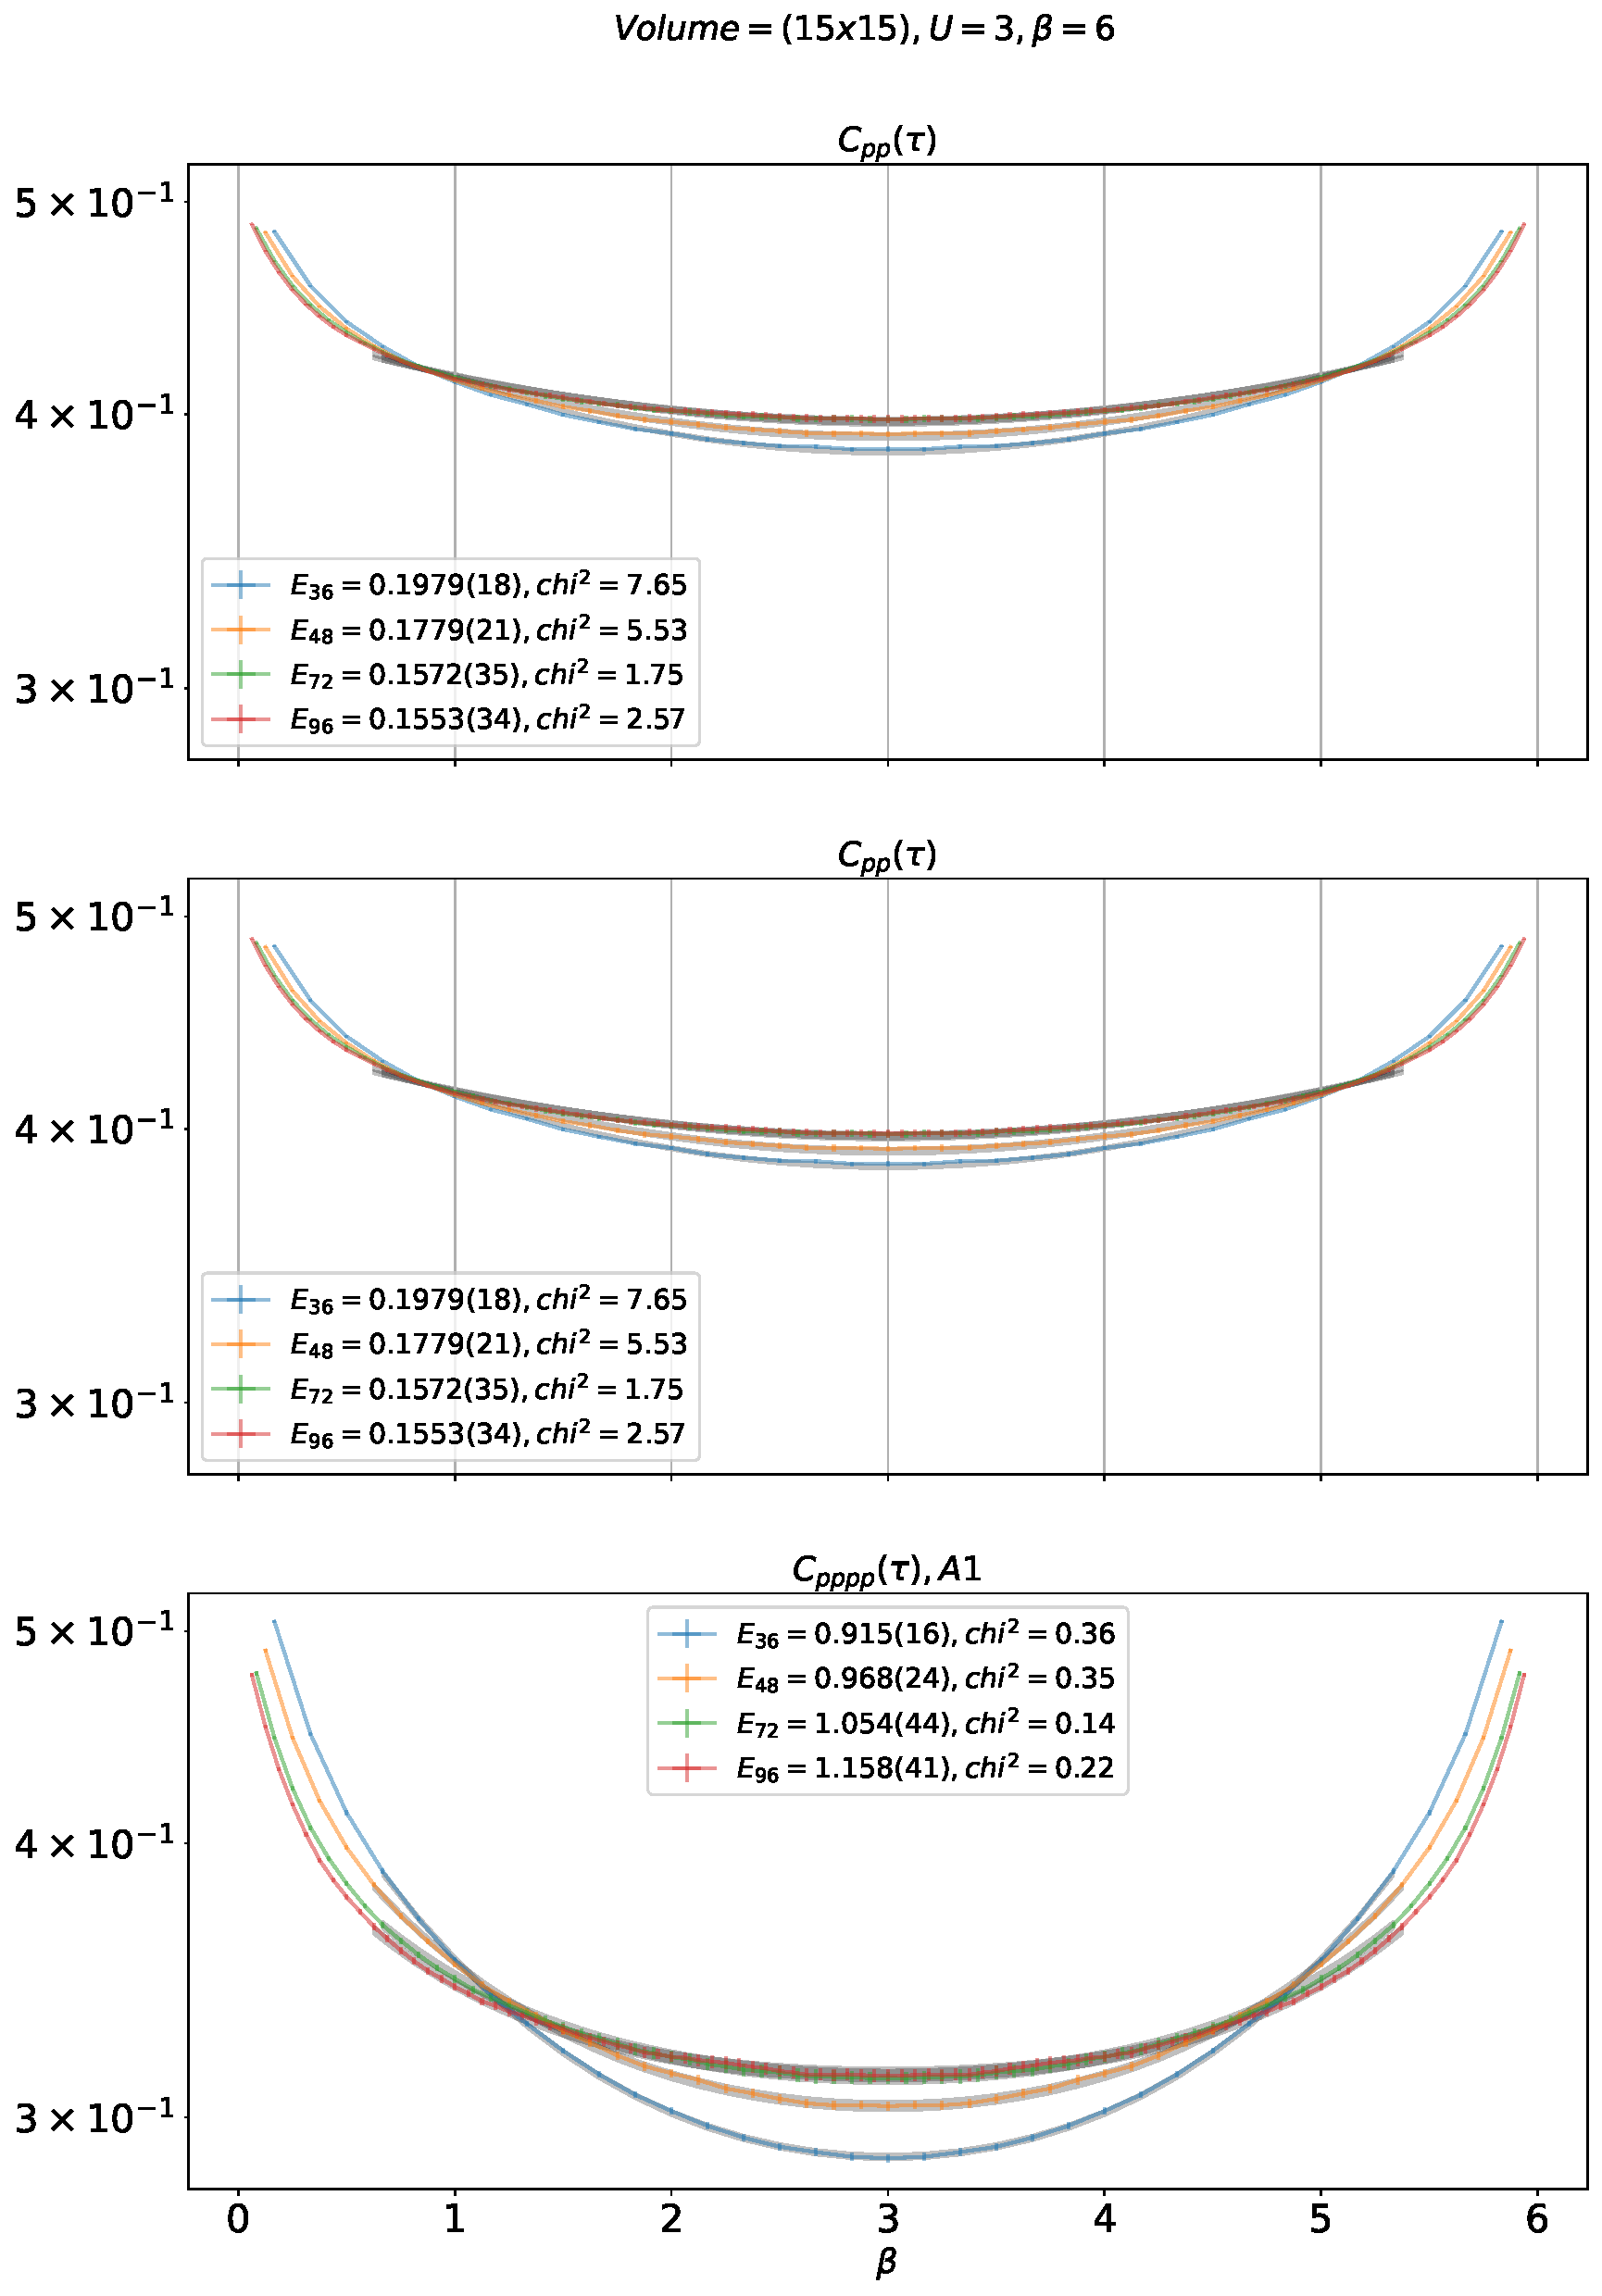
\includegraphics[width=\linewidth]{pppp-0-A1_15x15_U3_B6.pdf}
  \end{subfigure}%
  \begin{subfigure}{.5\textwidth}
    \centering
    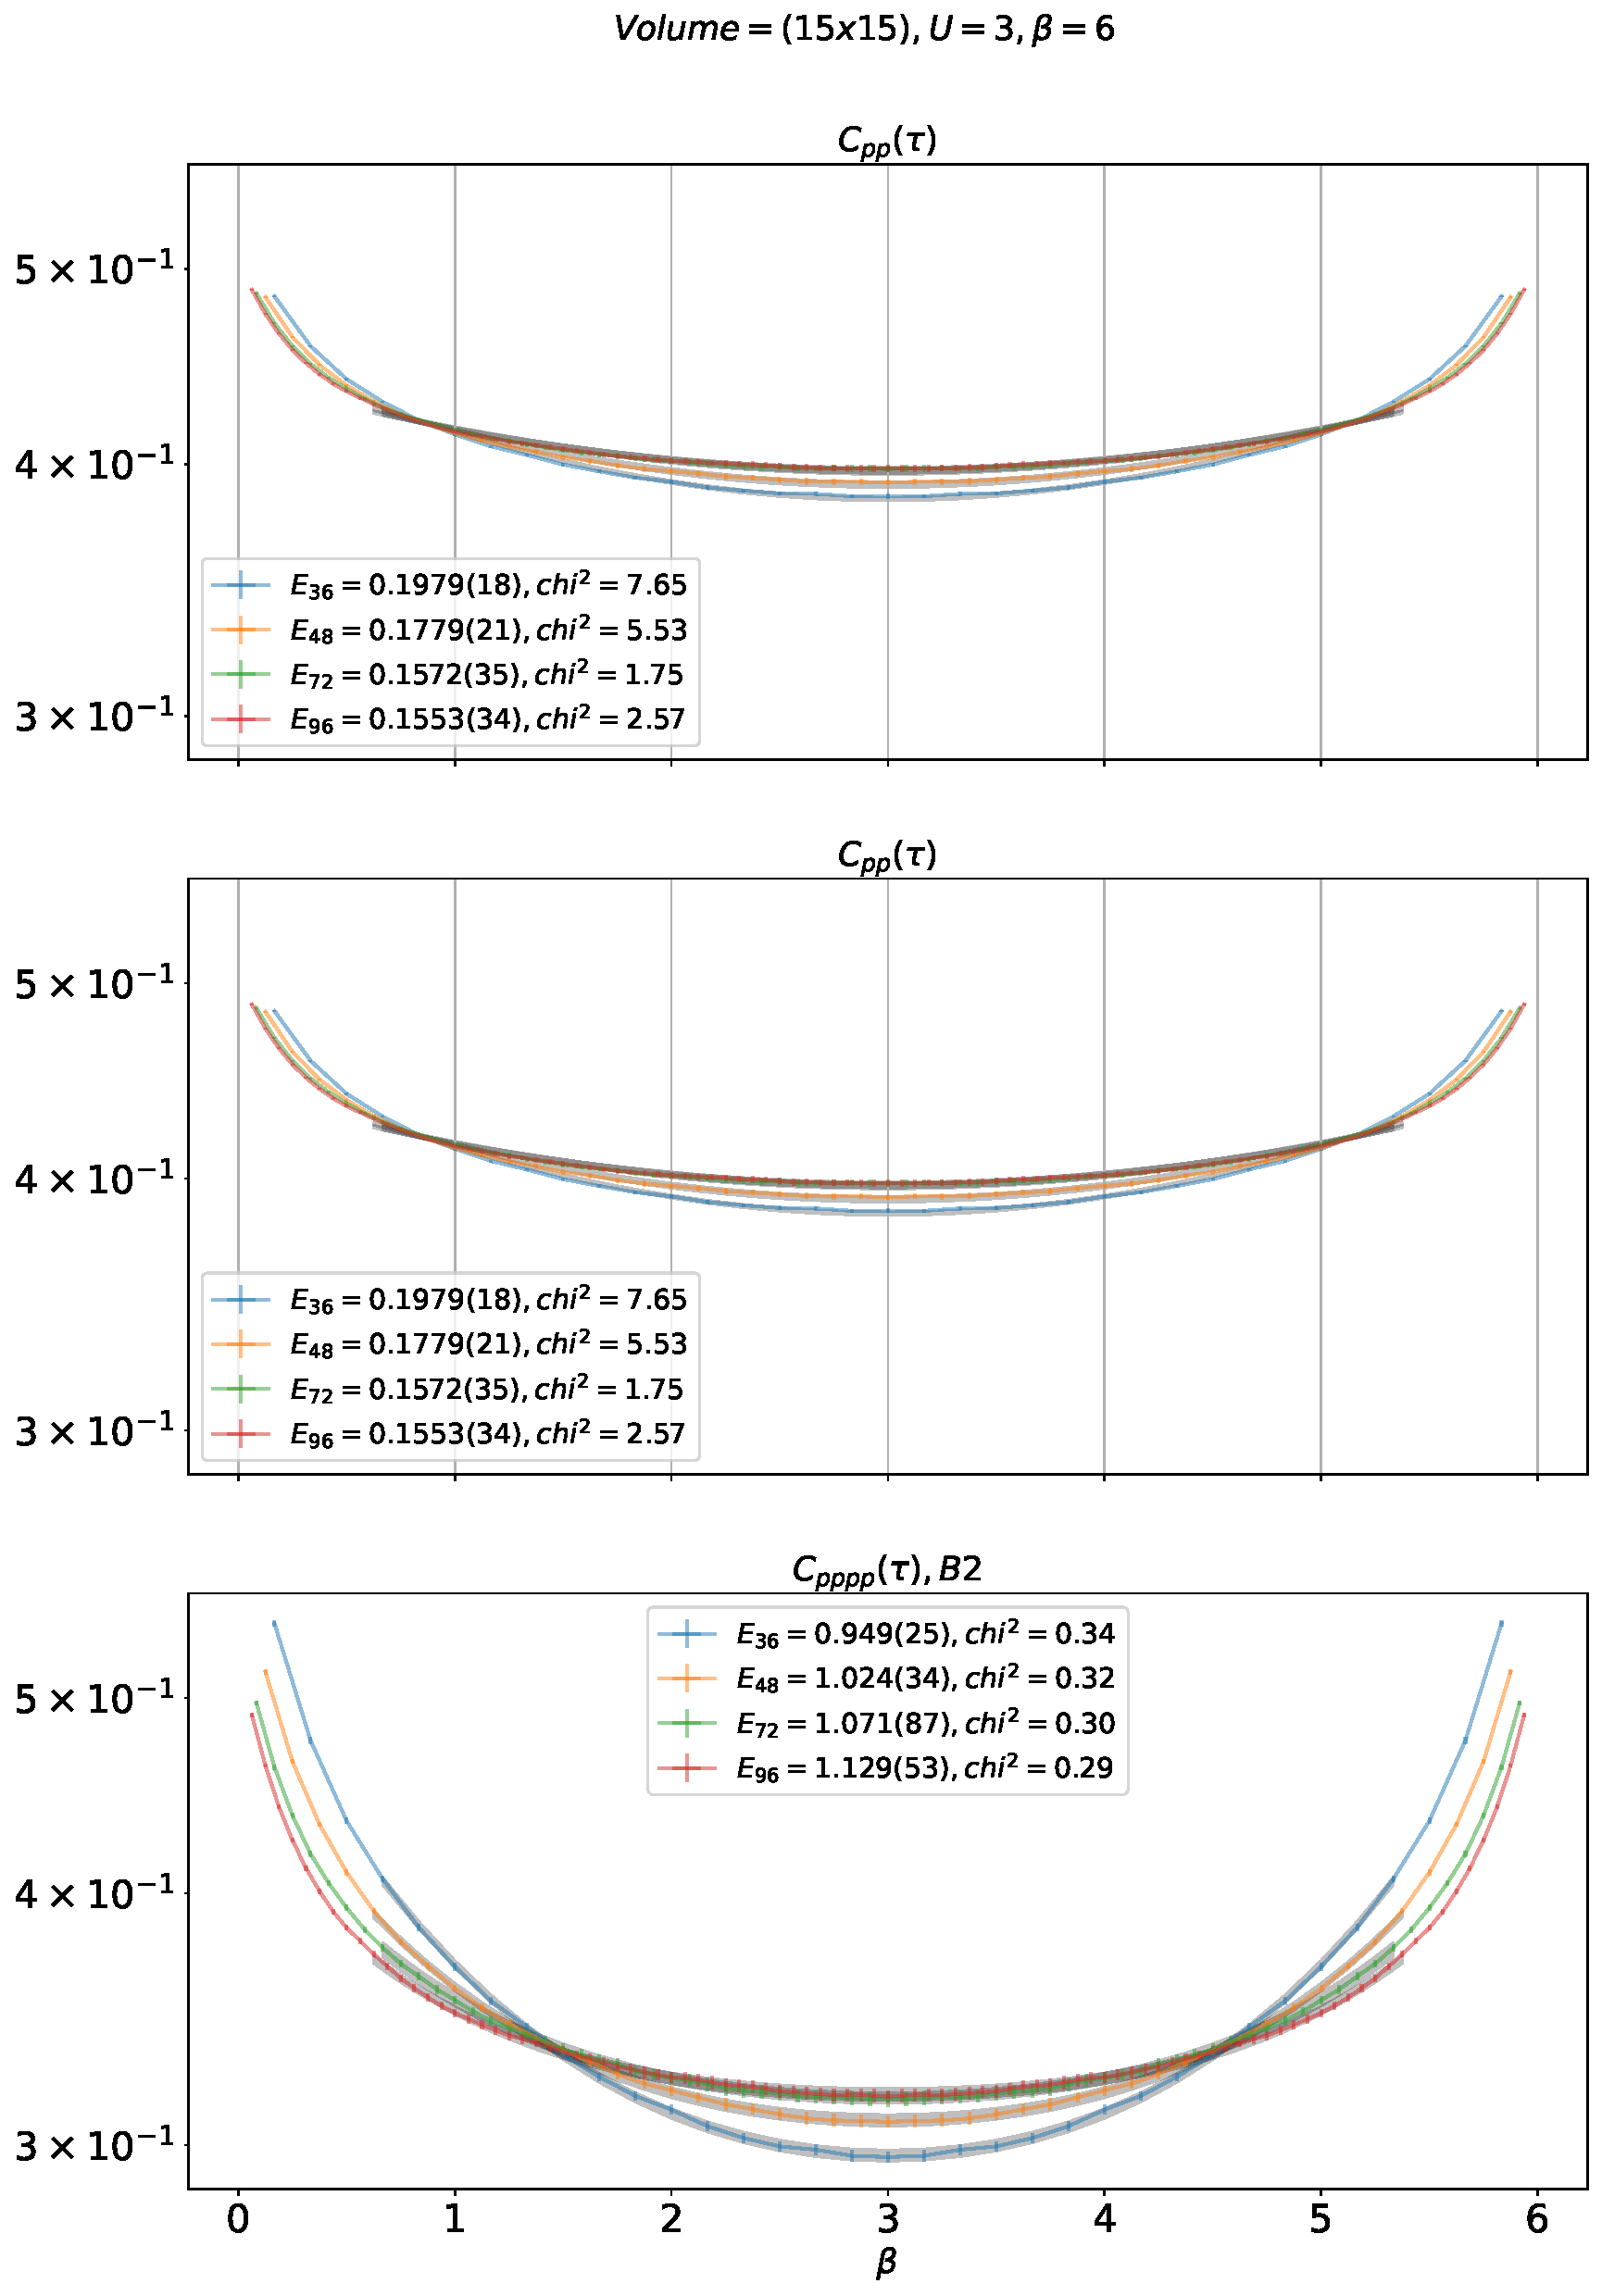
\includegraphics[width=\linewidth]{pppp-0-B2_15x15_U3_B6.pdf}
  \end{subfigure}
  \begin{subfigure}{.5\textwidth}
      \centering
      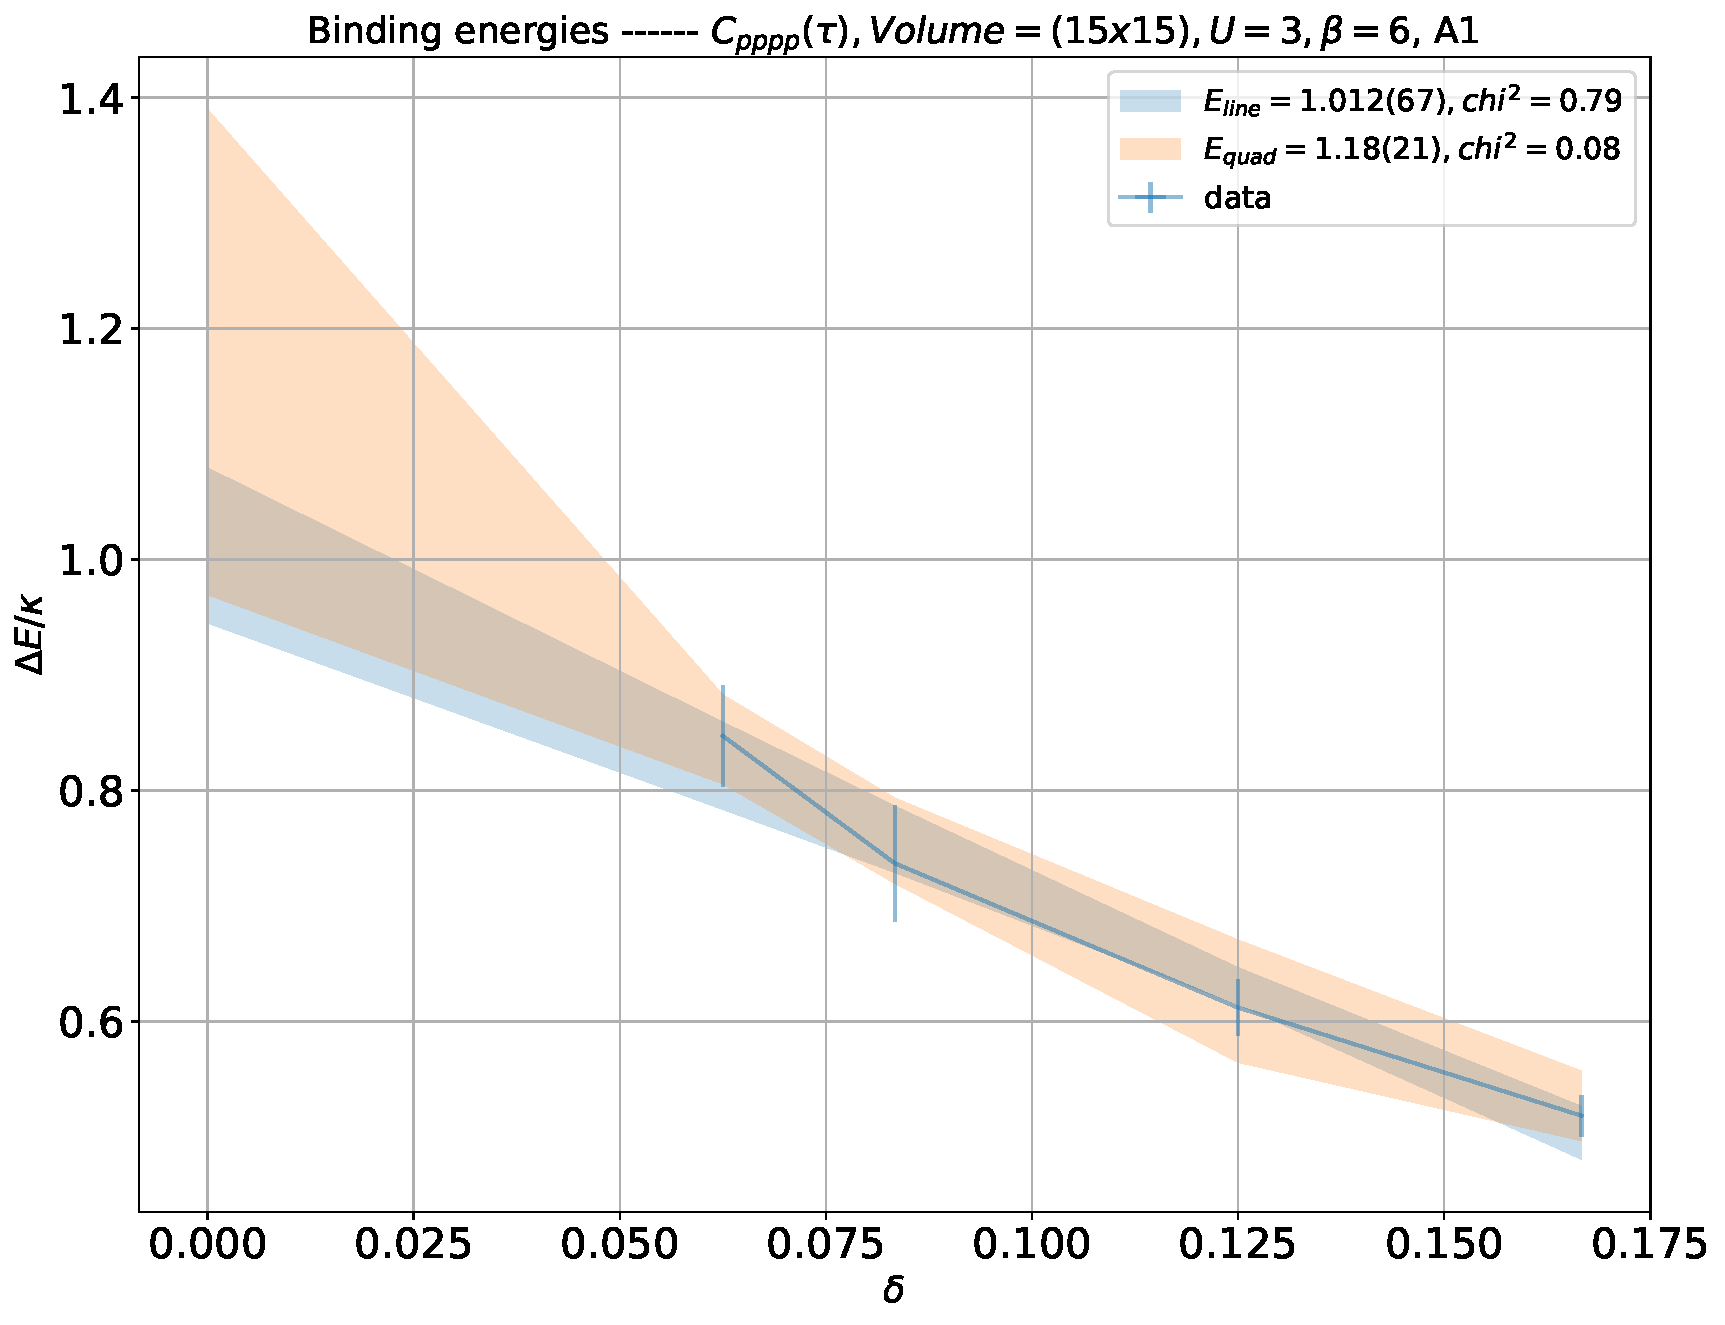
\includegraphics[width=\linewidth]{pppp-0-A1_15x15_U3_B6_cont.pdf}
  \end{subfigure}
  \begin{subfigure}{.5\textwidth}
      \centering
      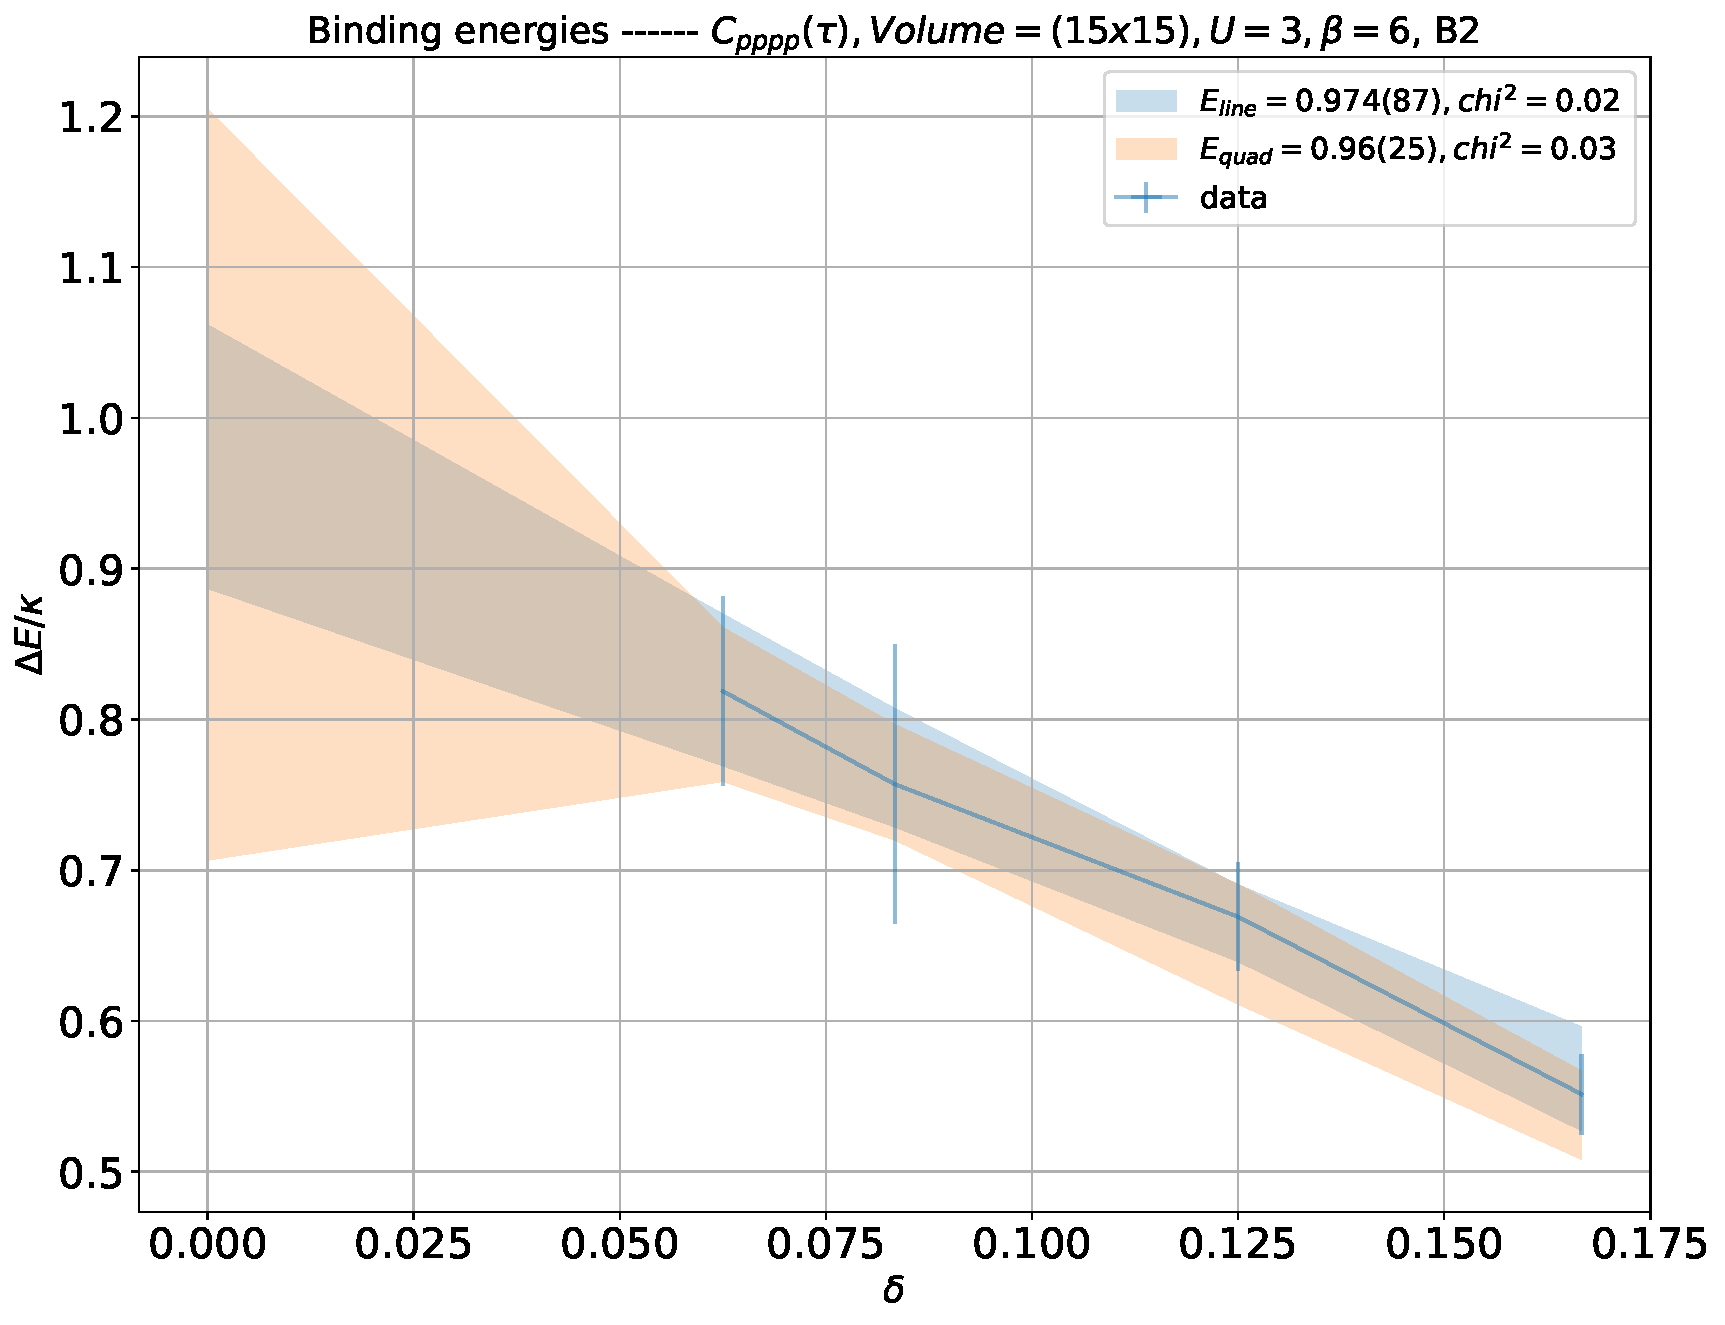
\includegraphics[width=\linewidth]{pppp-0-B2_15x15_U3_B6_cont.pdf}
  \end{subfigure}
  \caption{Binding energy extraction of the particle-particle pair at both irreducible representations, where we fit one- and two-body correlators for every $N_t$. This is followed by fitting a linear and a quadratic functions to the $\Delta E_{N_t}$ in order to extrapolate to the continuum limit ($N_t\to\infty$).}
  \label{fig:fig9}
\end{figure}

\begin{figure}
  \begin{subfigure}{.5\textwidth}
    \centering
    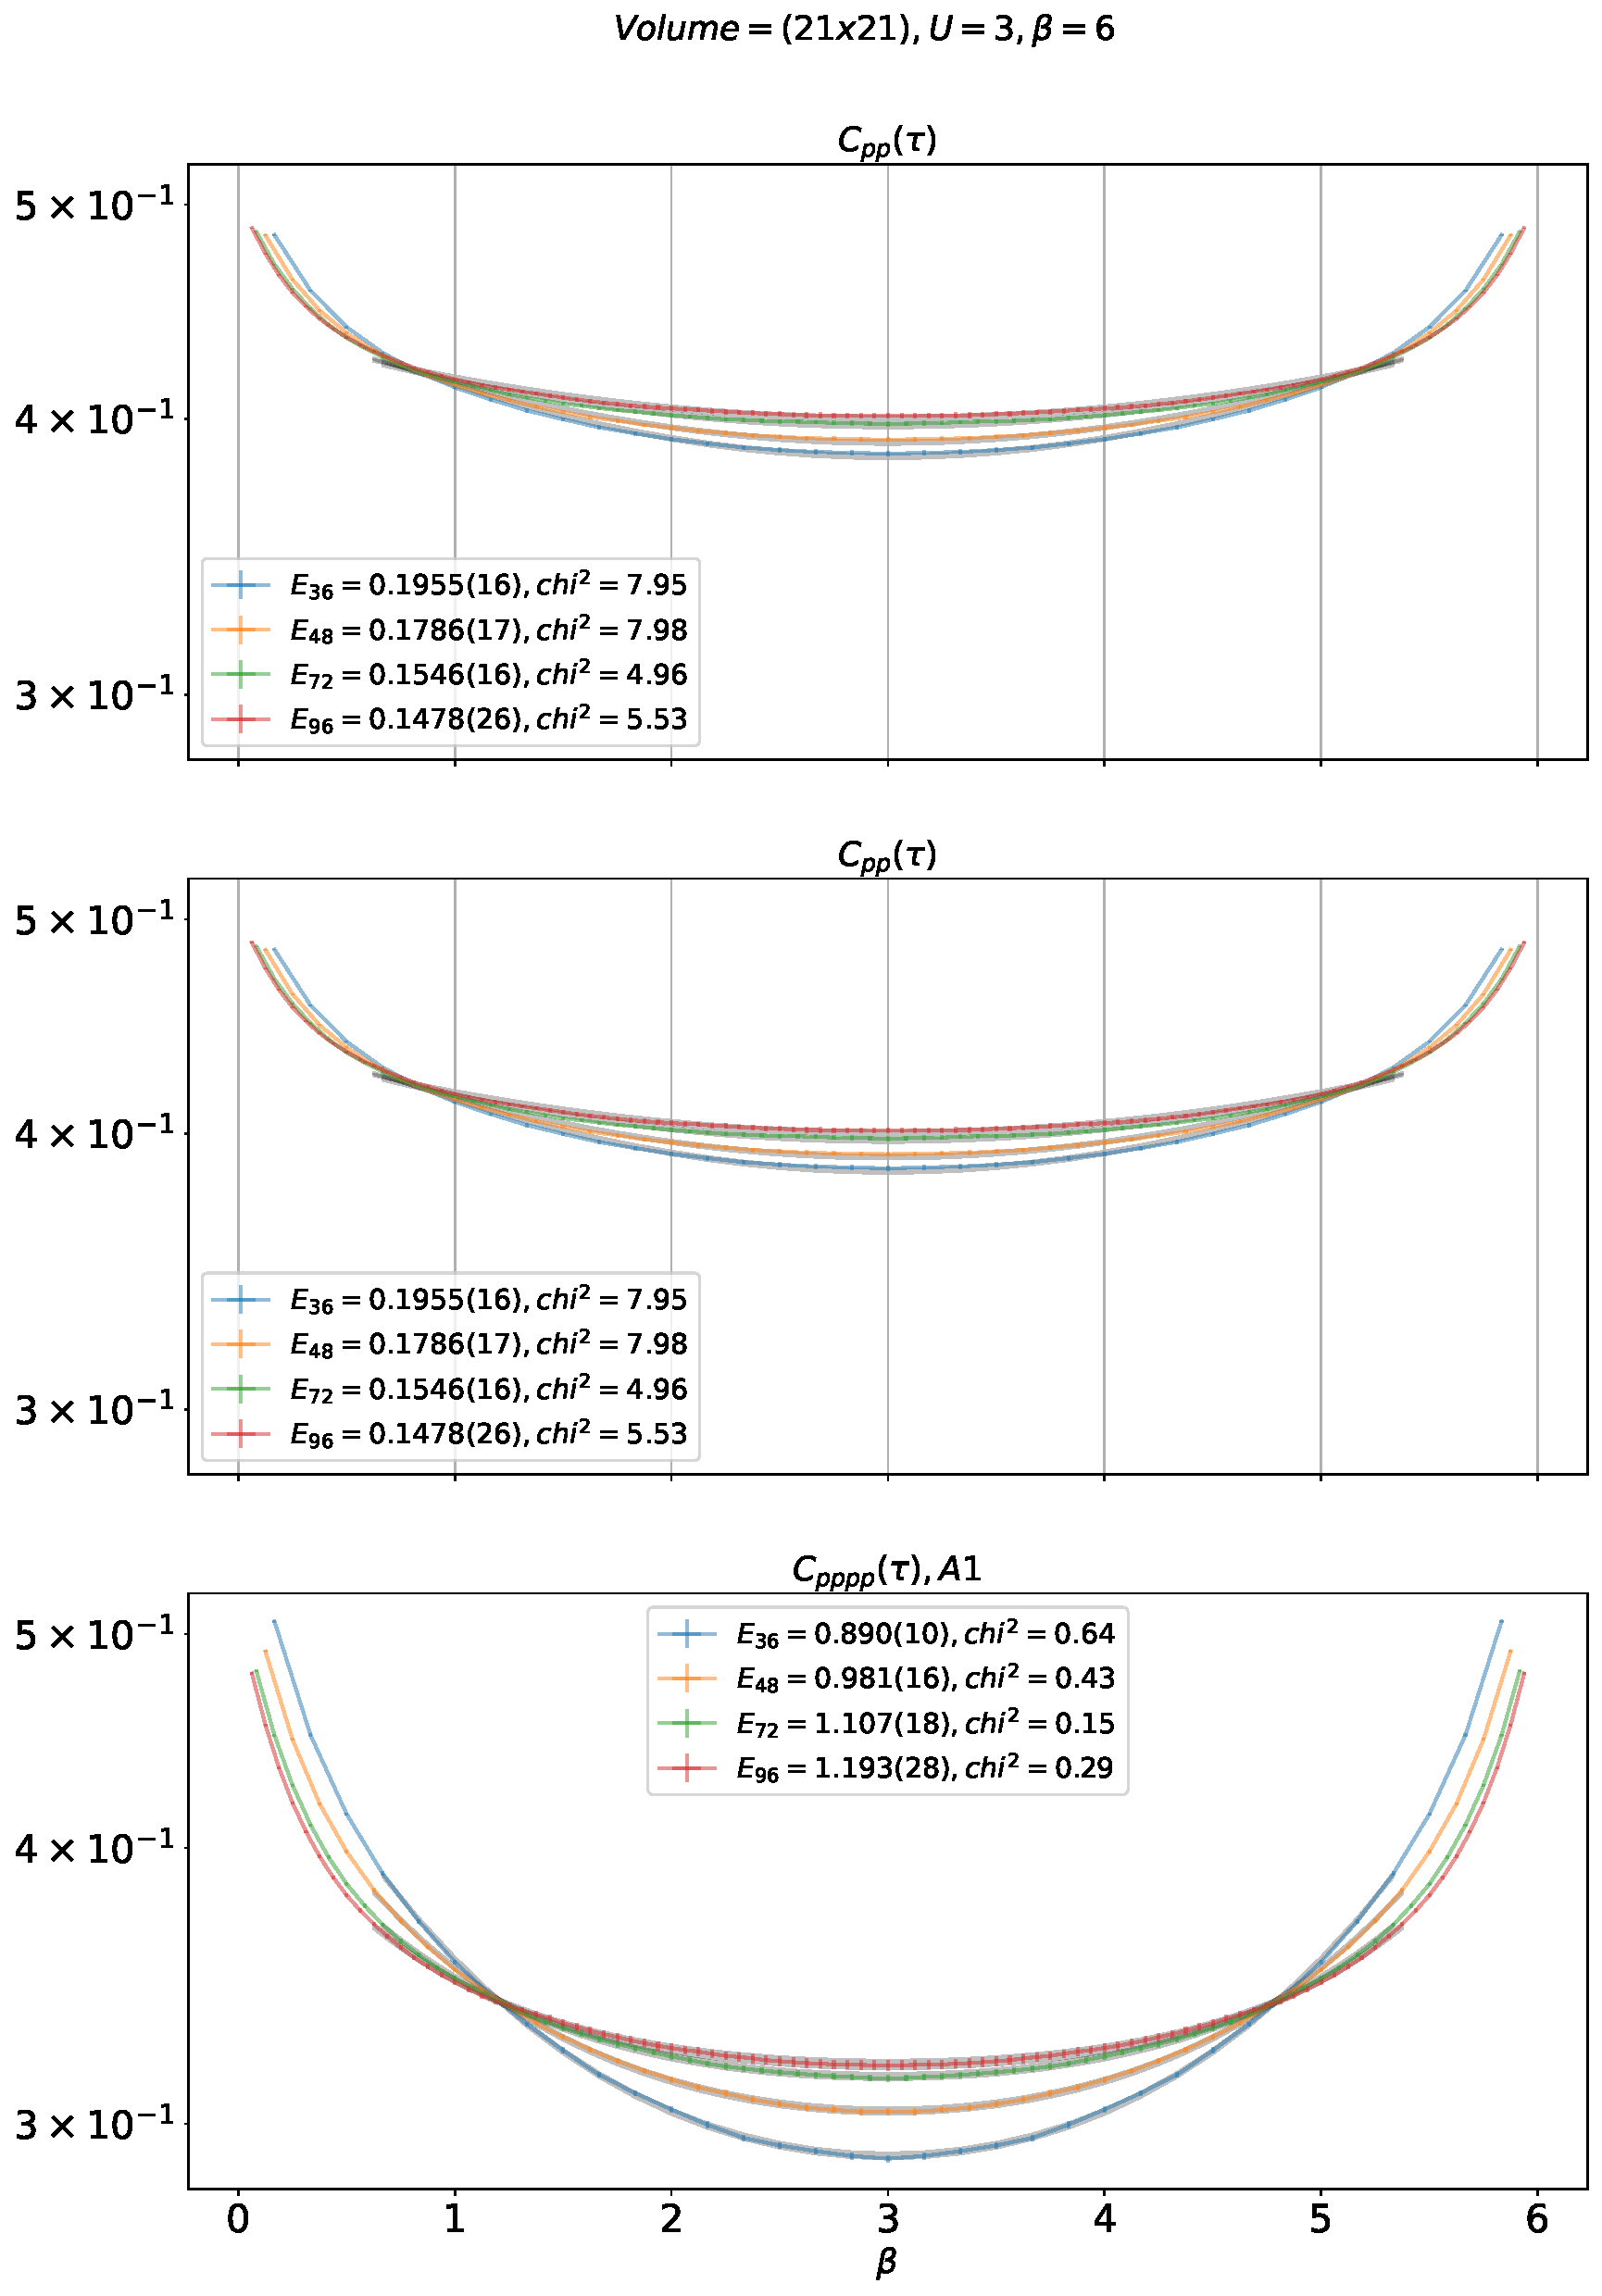
\includegraphics[width=\linewidth]{pppp-0-A1_21x21_U3_B6.pdf}
  \end{subfigure}%
  \begin{subfigure}{.5\textwidth}
    \centering
    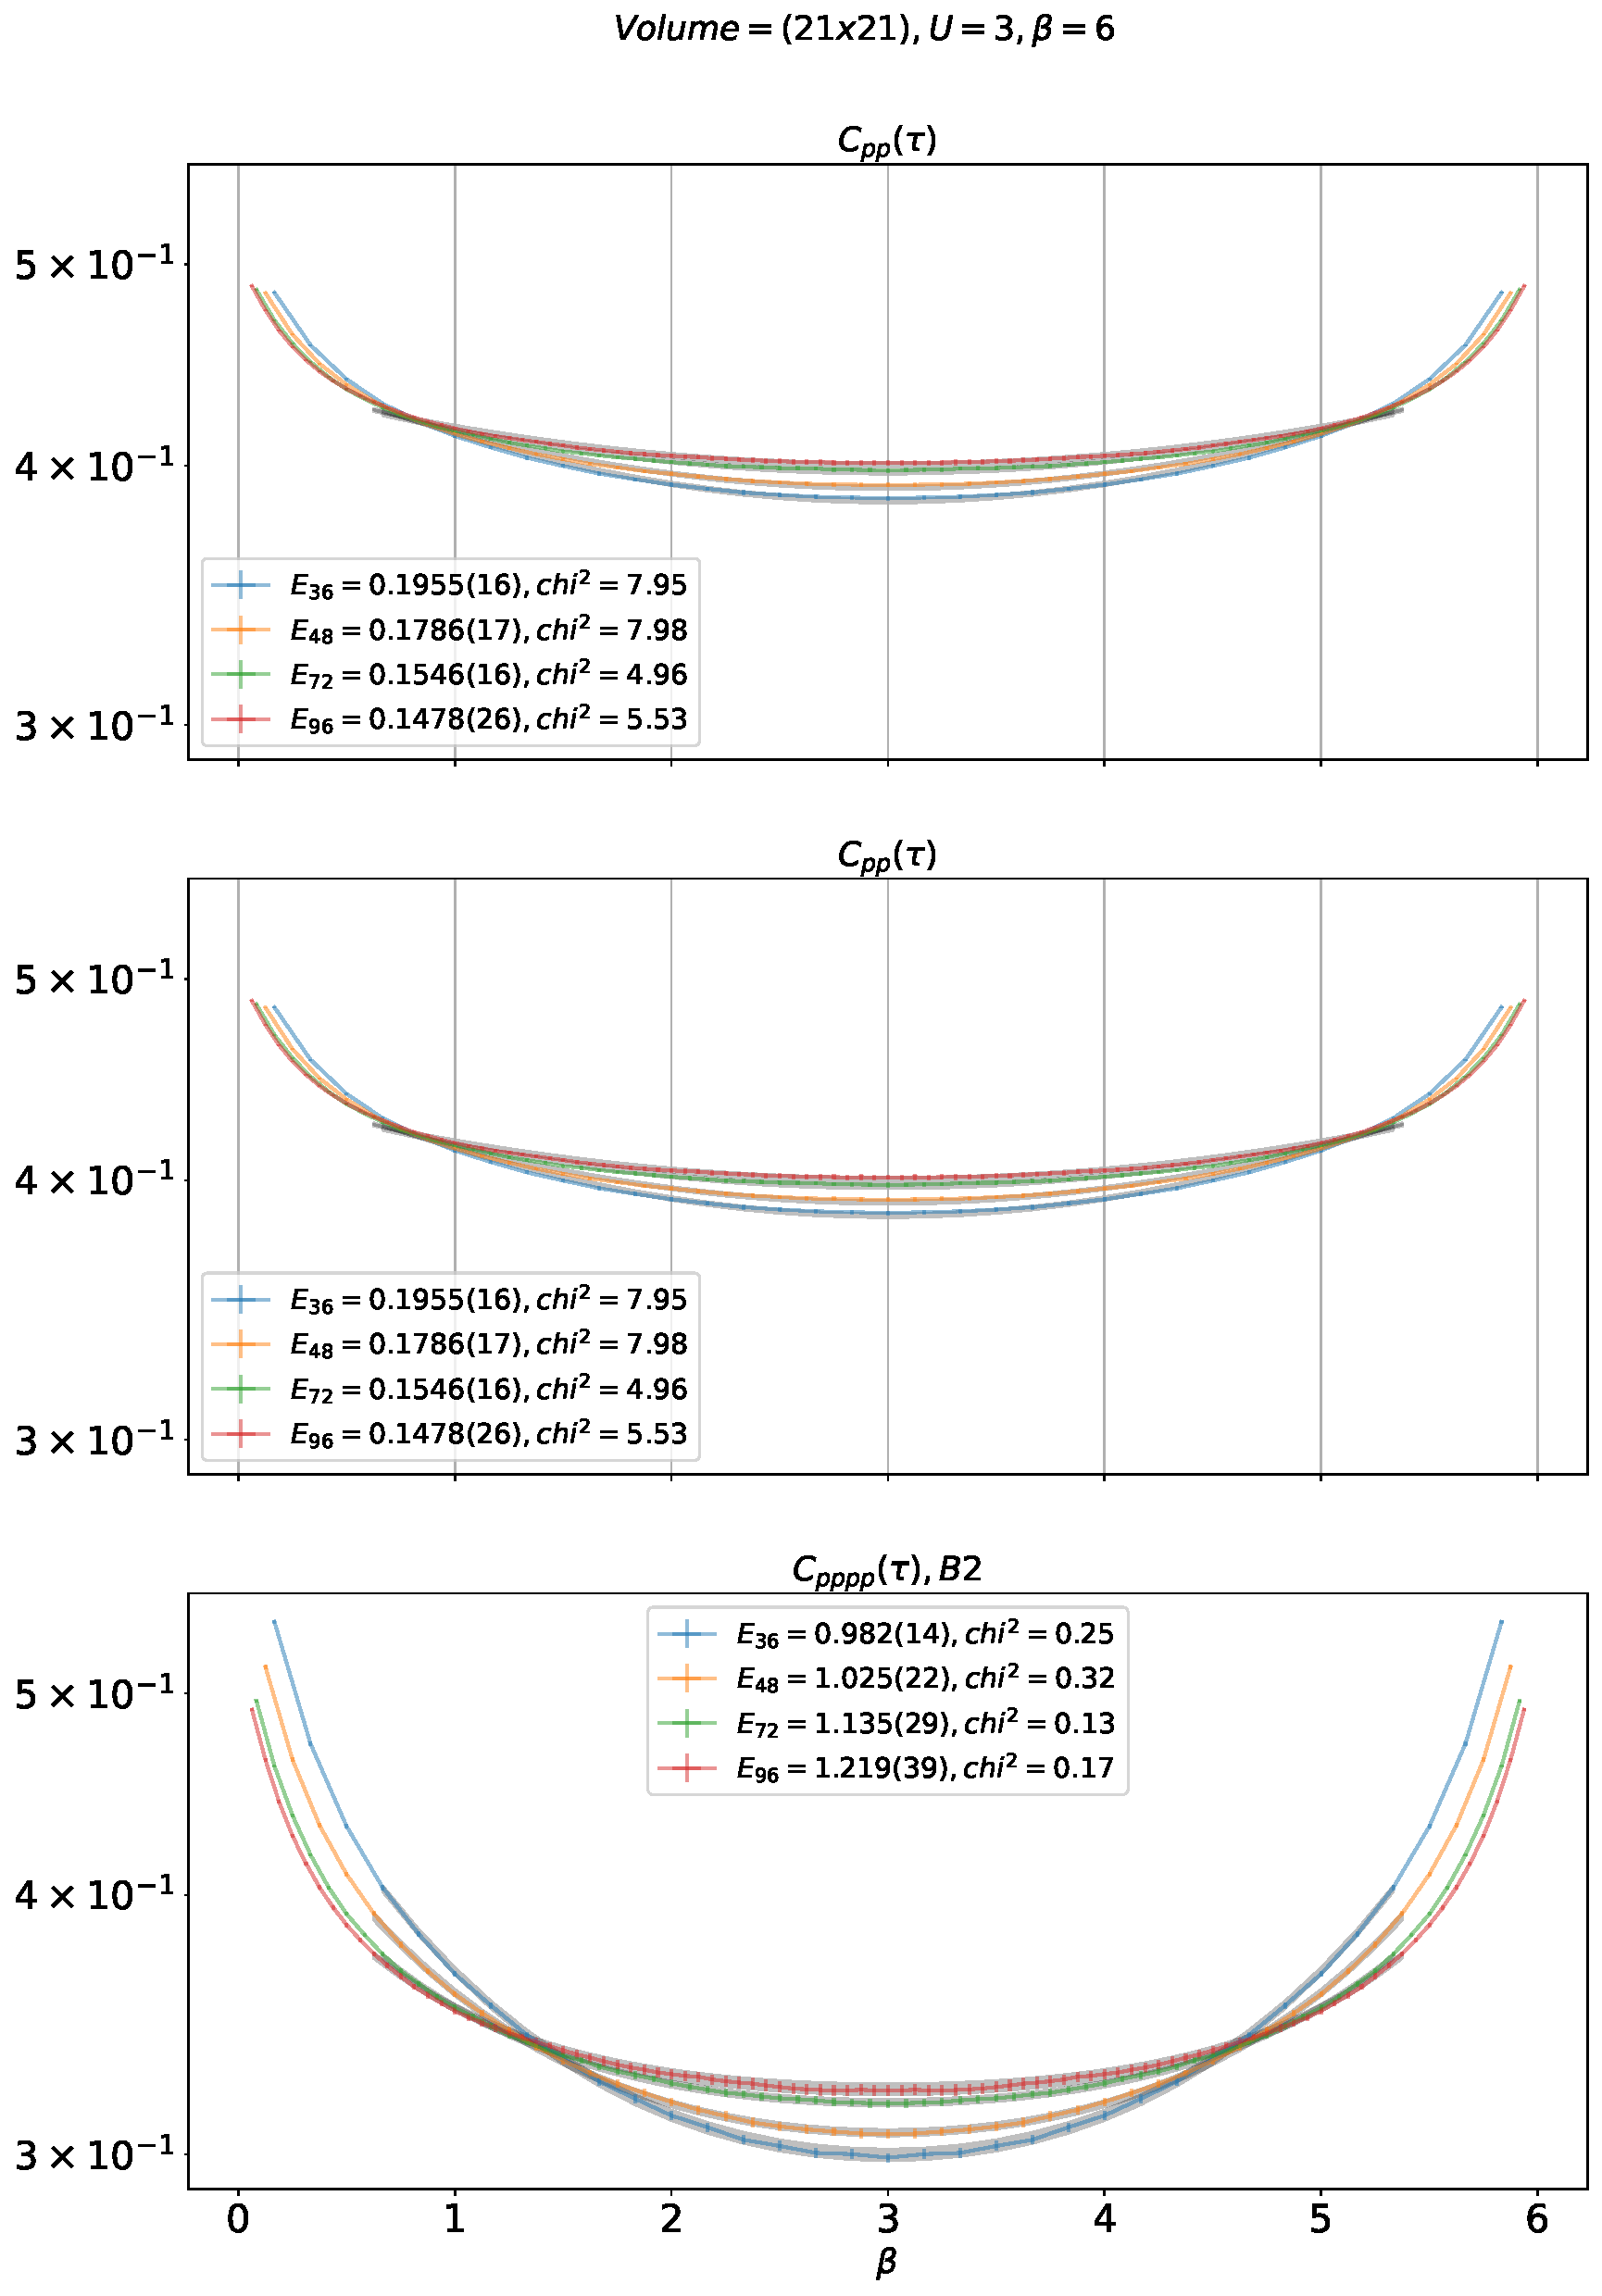
\includegraphics[width=\linewidth]{pppp-0-B2_21x21_U3_B6.pdf}
  \end{subfigure}
  \begin{subfigure}{.5\textwidth}
      \centering
      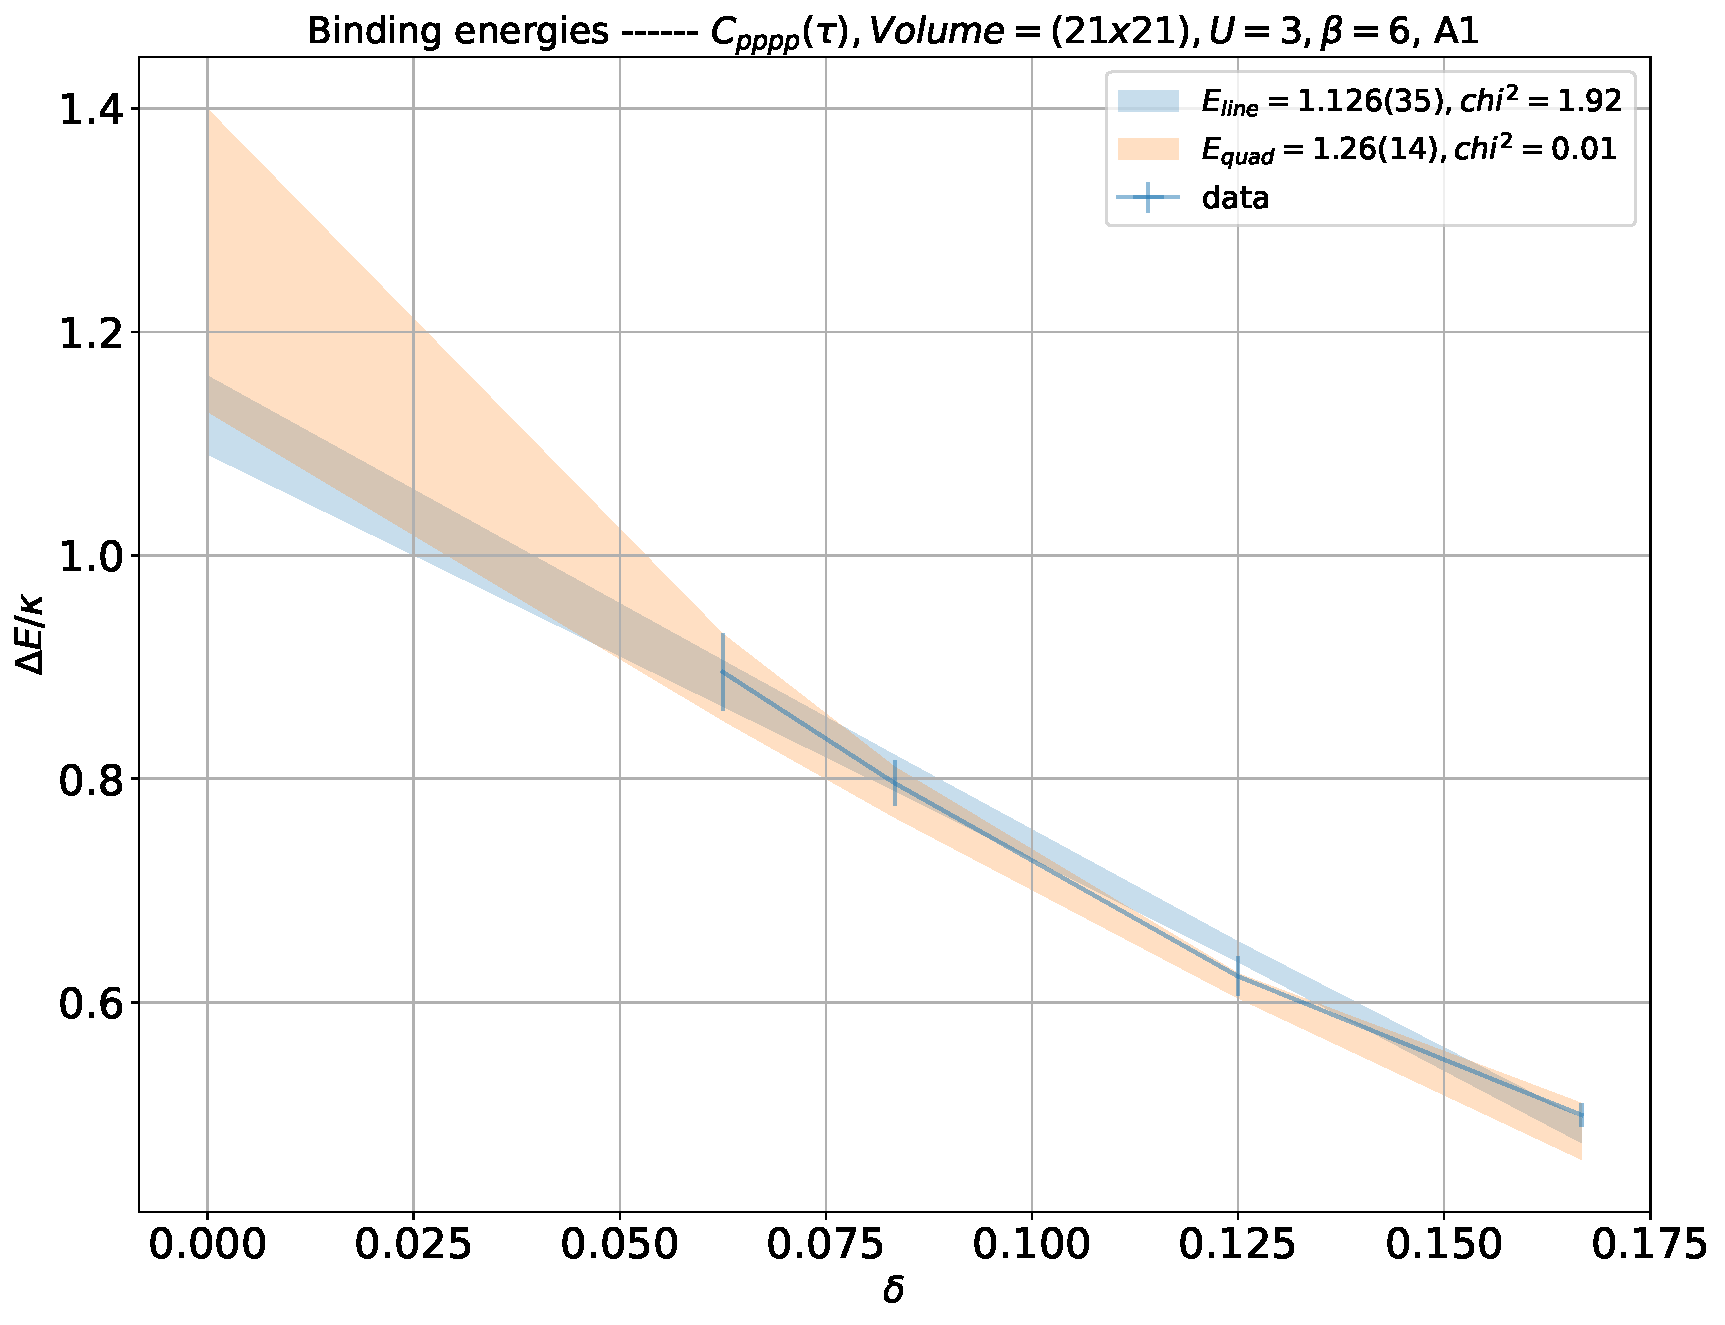
\includegraphics[width=\linewidth]{pppp-0-A1_21x21_U3_B6_cont.pdf}
  \end{subfigure}
  \begin{subfigure}{.5\textwidth}
      \centering
      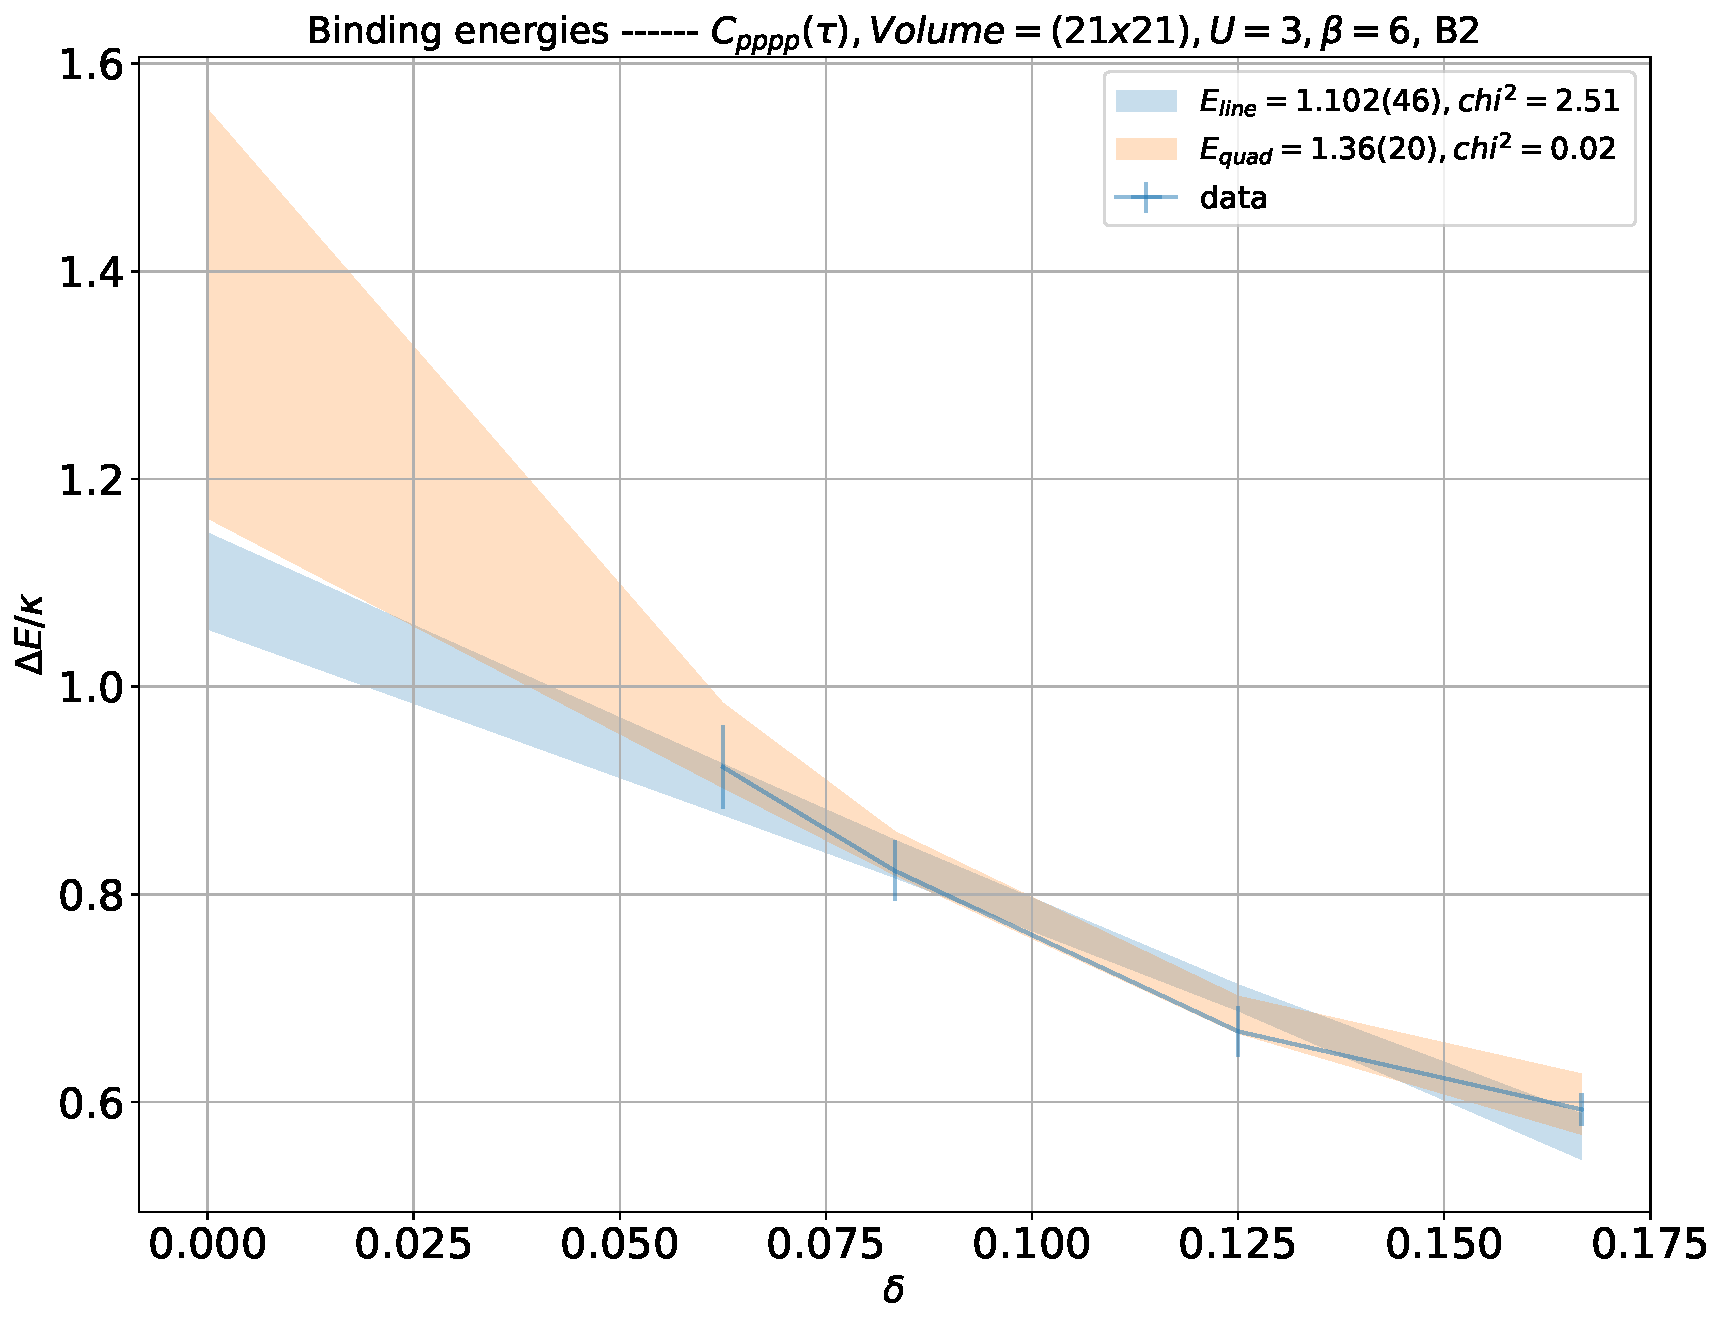
\includegraphics[width=\linewidth]{pppp-0-B2_21x21_U3_B6_cont.pdf}
  \end{subfigure}
  \caption{Binding energy extraction of the particle-particle pair at both irreducible representations, where we fit one- and two-body correlators for every $N_t$. This is followed by fitting a linear and a quadratic functions to the $\Delta E_{N_t}$ in order to extrapolate to the continuum limit ($N_t\to\infty$).}
  \label{fig:fig10}
\end{figure}
 
\begin{figure}
  \begin{subfigure}{.5\textwidth}
    \centering
    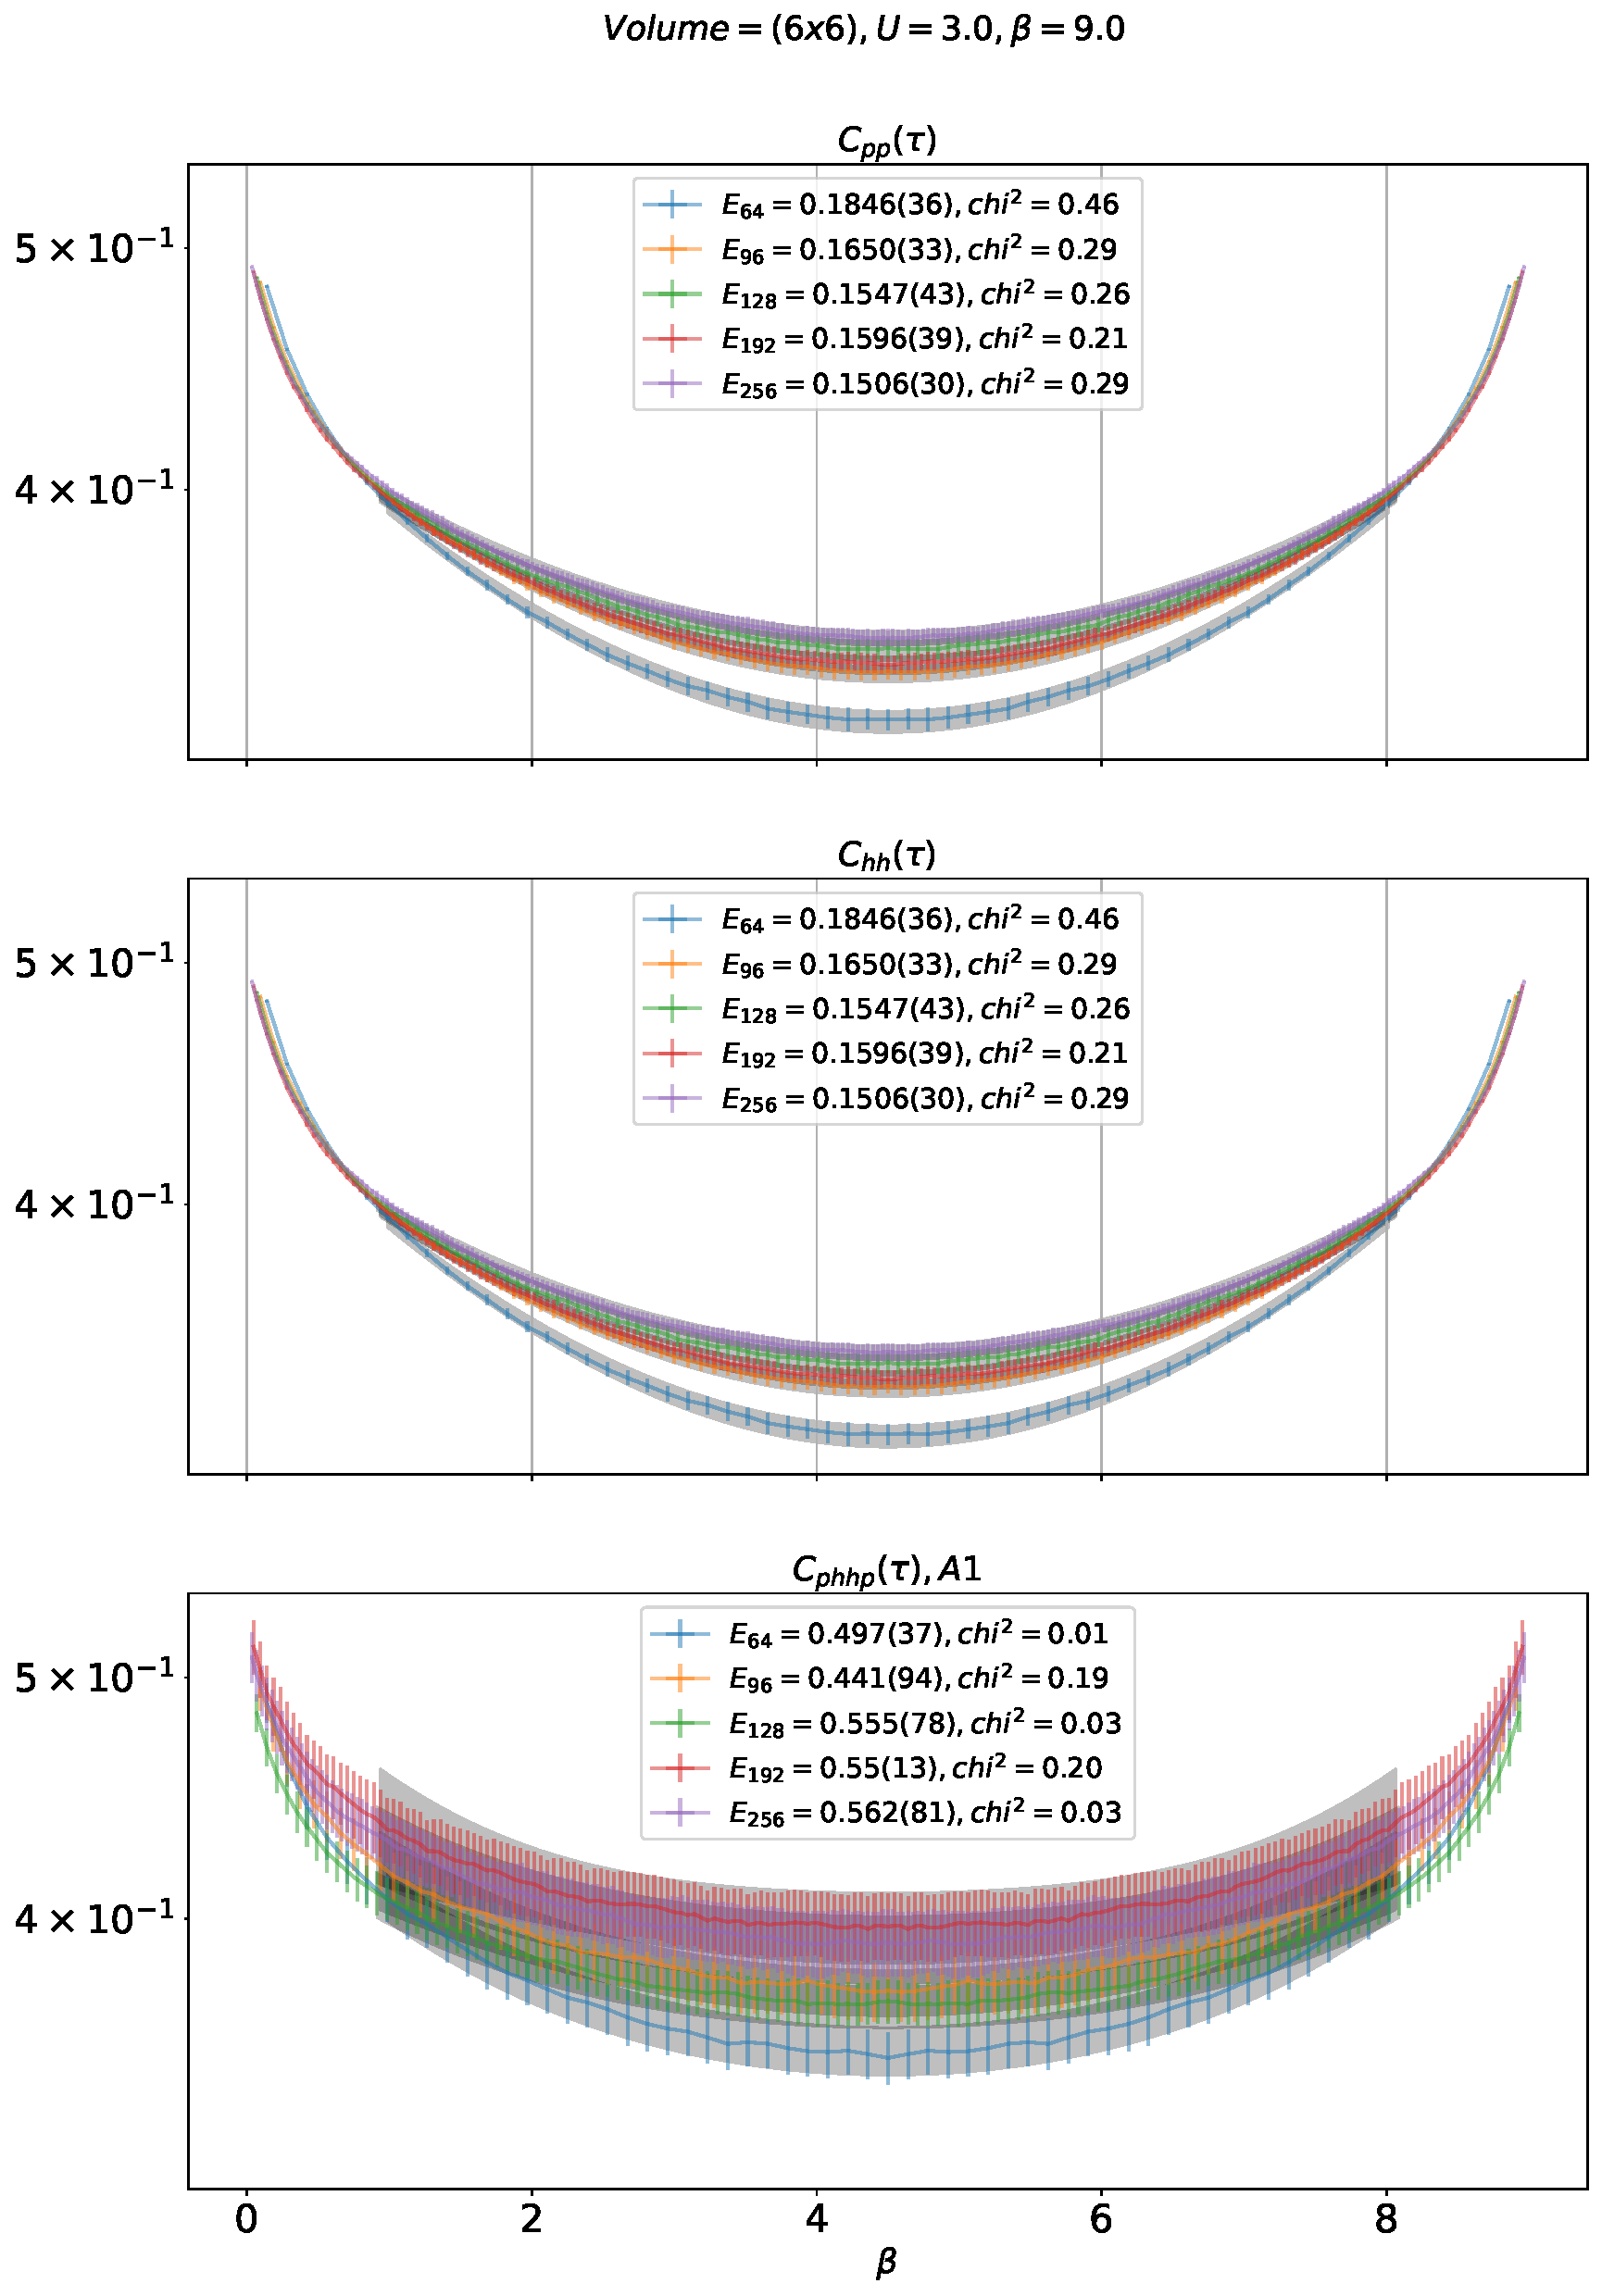
\includegraphics[width=\linewidth]{phhp-0-A1_6x6_U3.0_B9.0.pdf}
  \end{subfigure}%
  \begin{subfigure}{.5\textwidth}
    \centering
    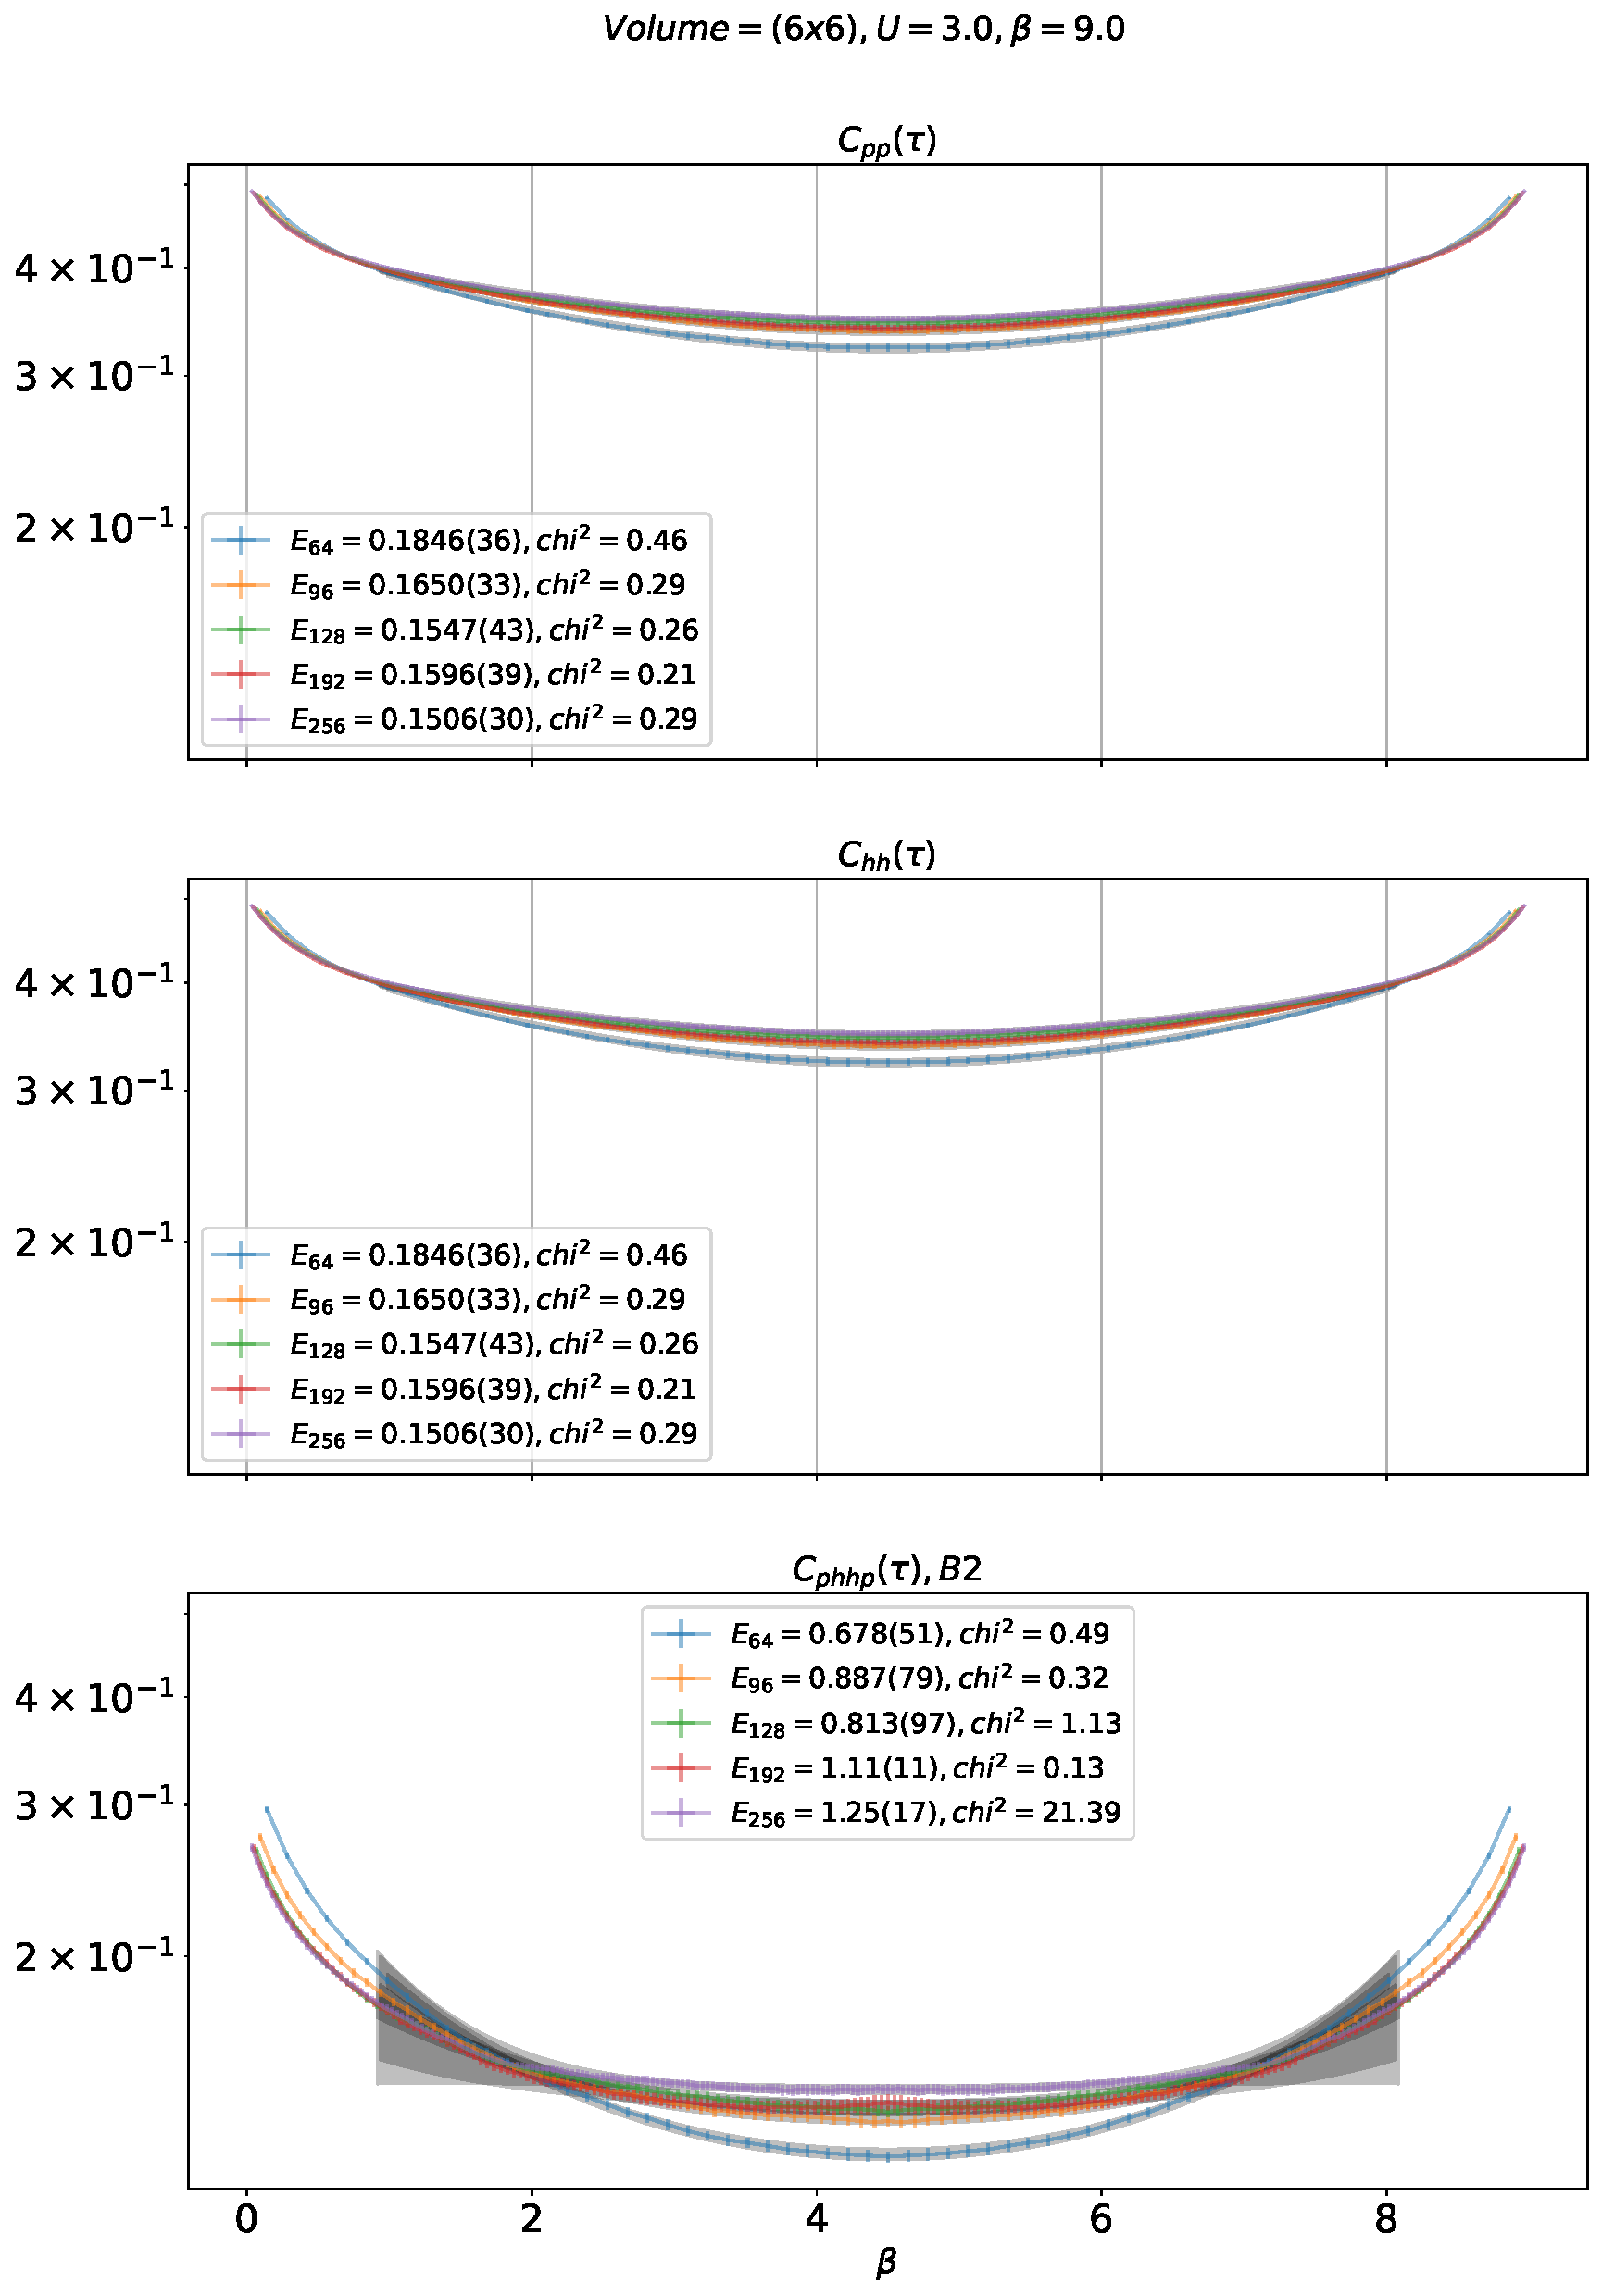
\includegraphics[width=\linewidth]{phhp-0-B2_6x6_U3.0_B9.0.pdf}
  \end{subfigure}
  \begin{subfigure}{.5\textwidth}
      \centering
      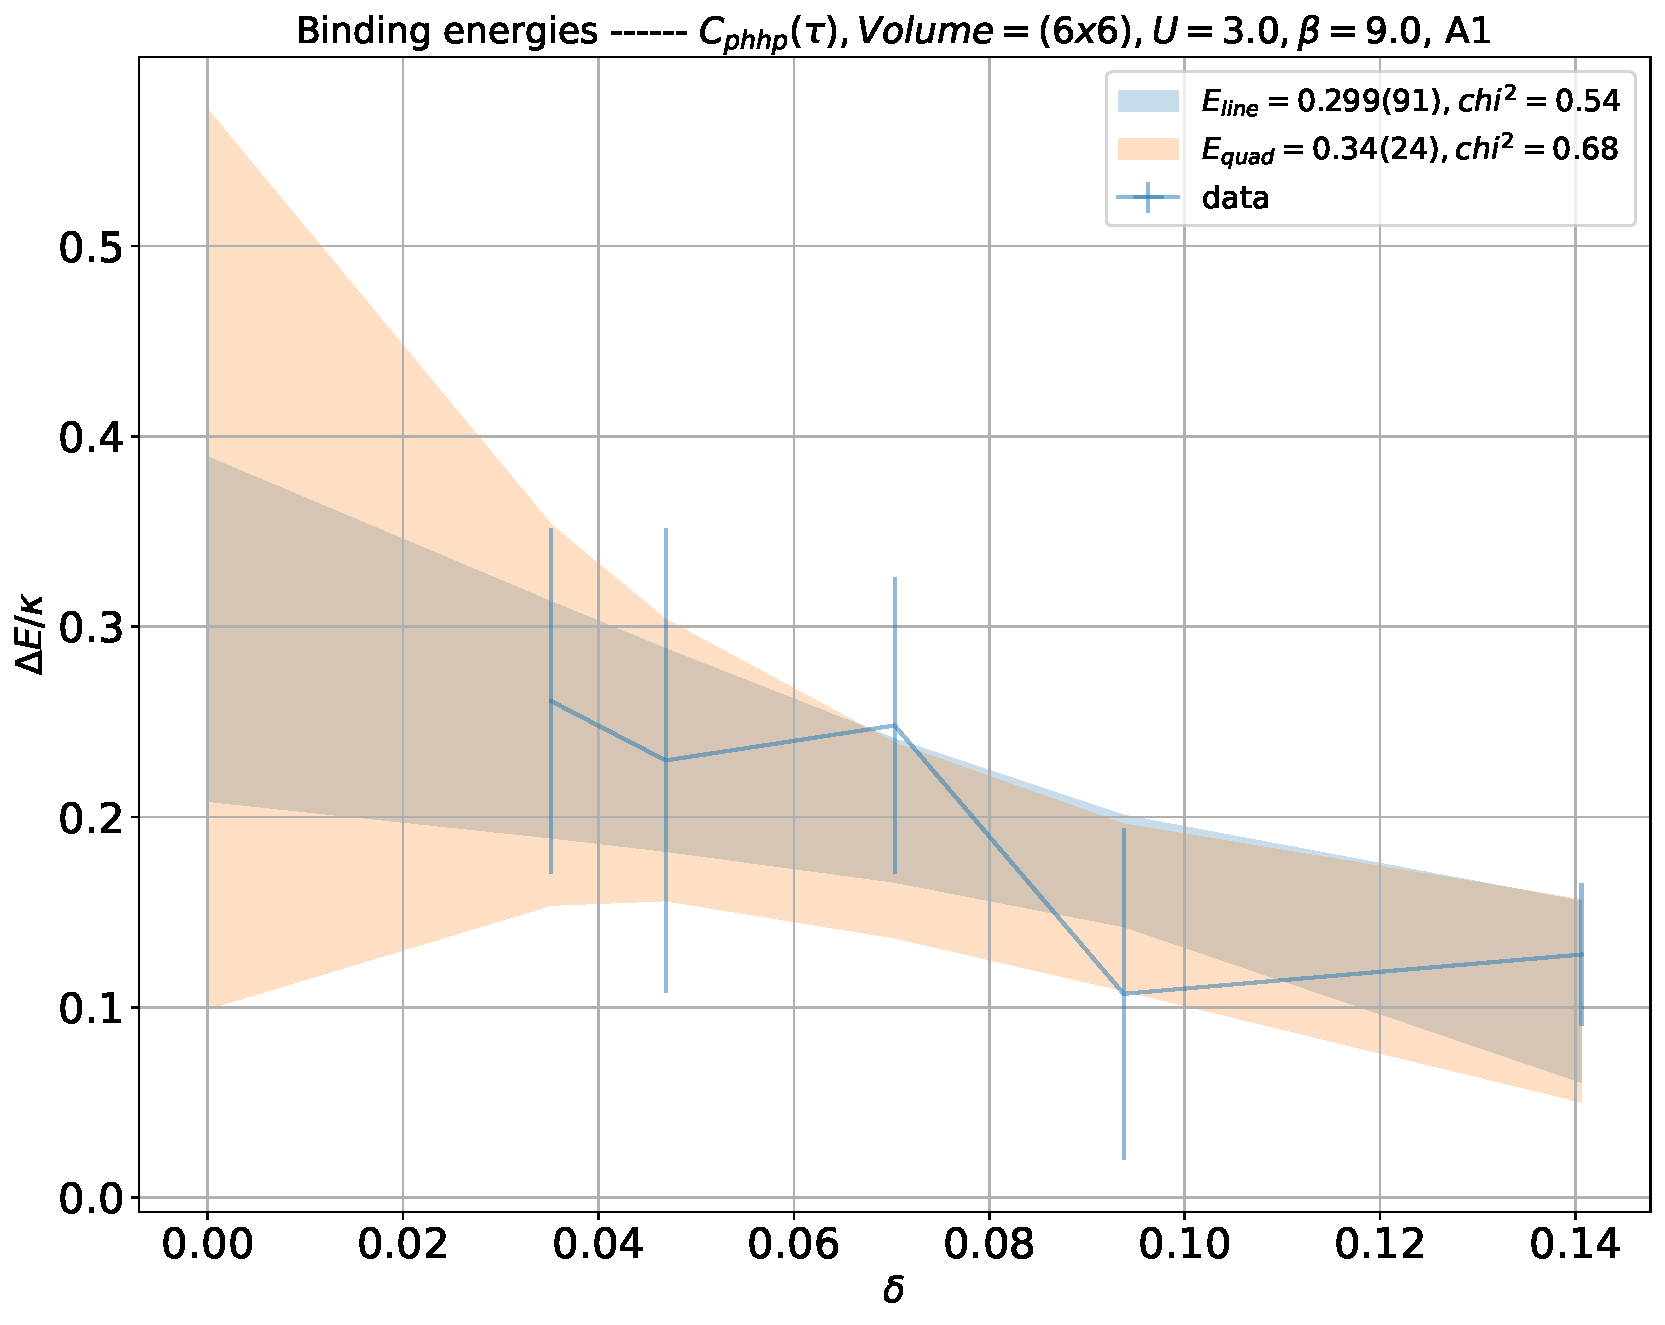
\includegraphics[width=\linewidth]{phhp-0-A1_6x6_U3.0_B9.0_cont.pdf}
  \end{subfigure}
  \begin{subfigure}{.5\textwidth}
      \centering
      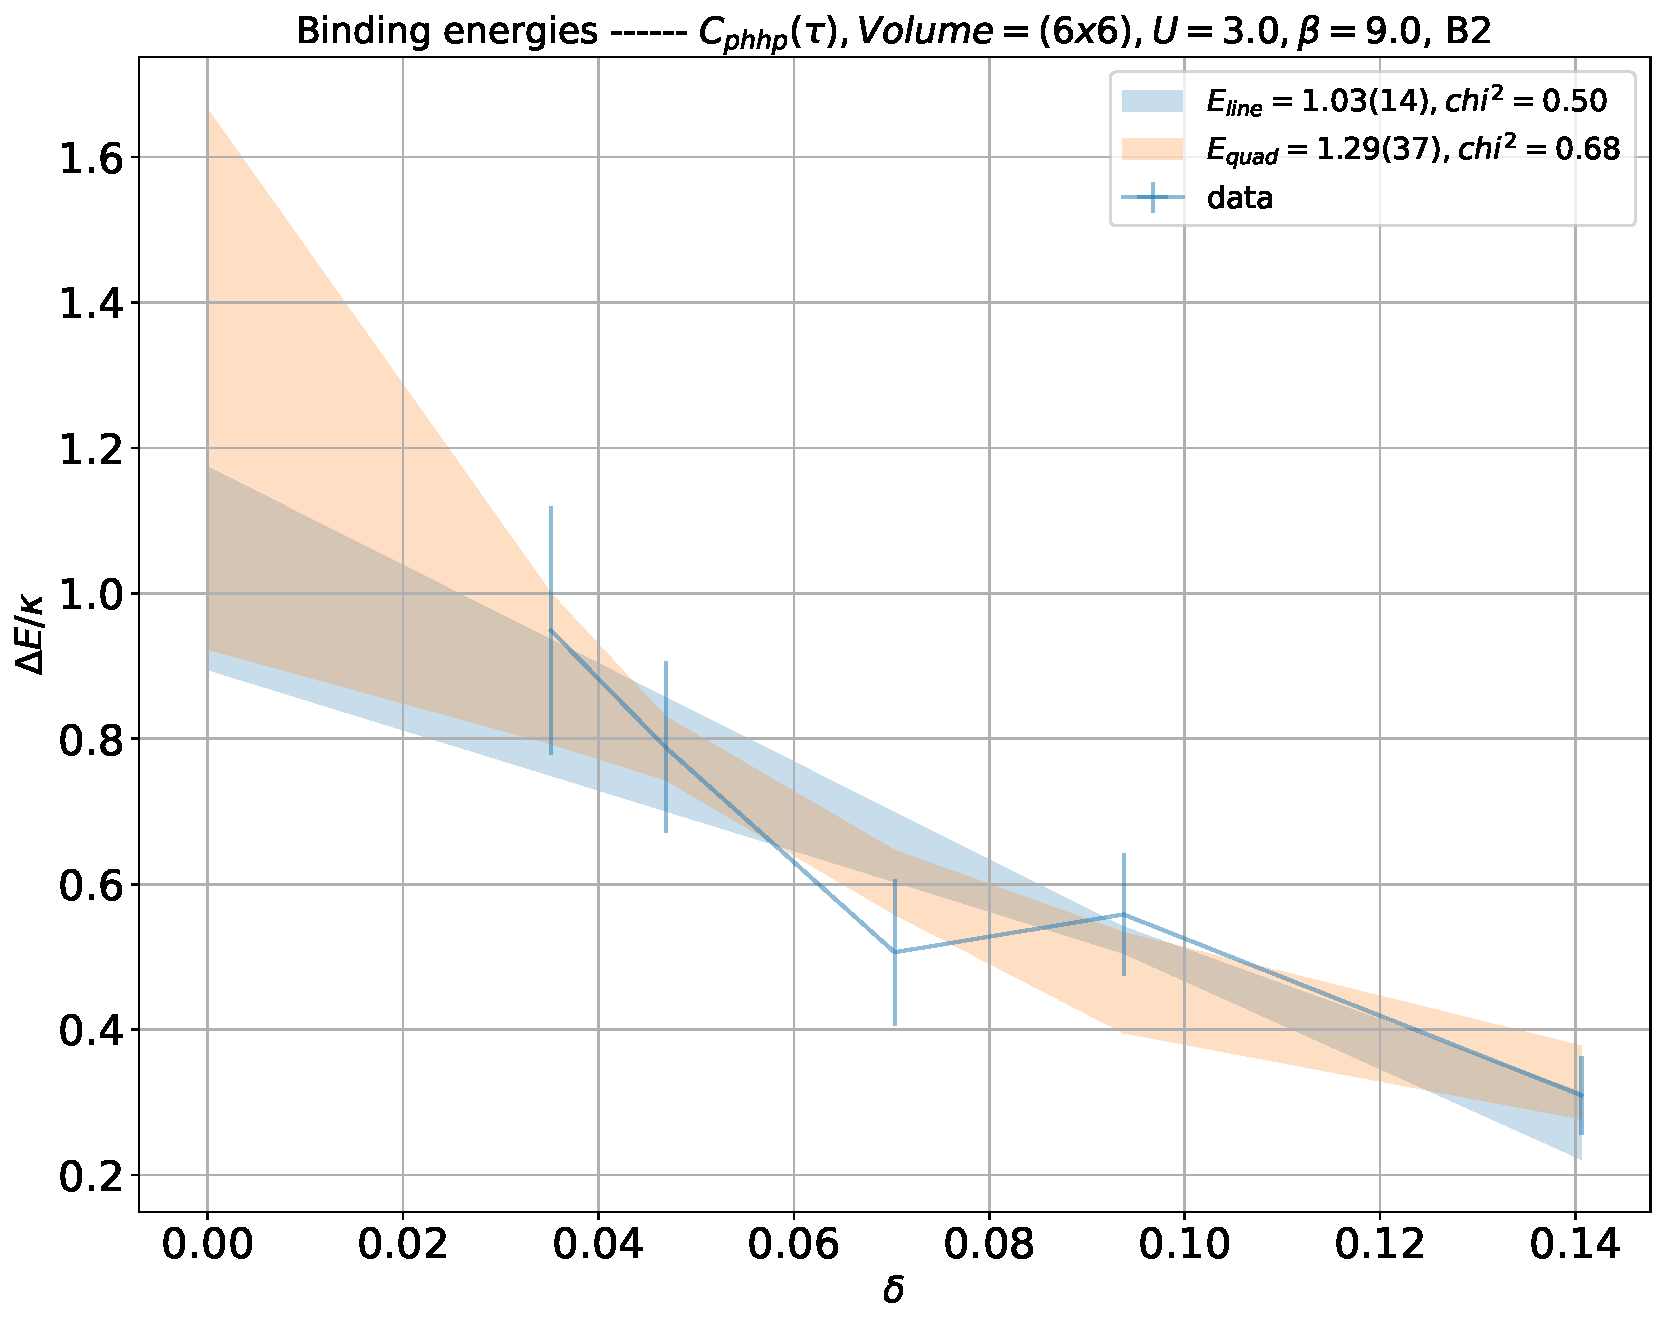
\includegraphics[width=\linewidth]{phhp-0-B2_6x6_U3.0_B9.0_cont.pdf}
  \end{subfigure}
  \caption{Binding energy extraction of the particle-hole pair at both irreducible representations, where we fit one- and two-body correlators for every $N_t$. This is followed by fitting a linear and a quadratic functions to the $\Delta E_{N_t}$ in order to extrapolate to the continuum limit ($N_t\to\infty$).}
  \label{fig:fig11}
\end{figure}

\begin{figure}
  \begin{subfigure}{.5\textwidth}
    \centering
    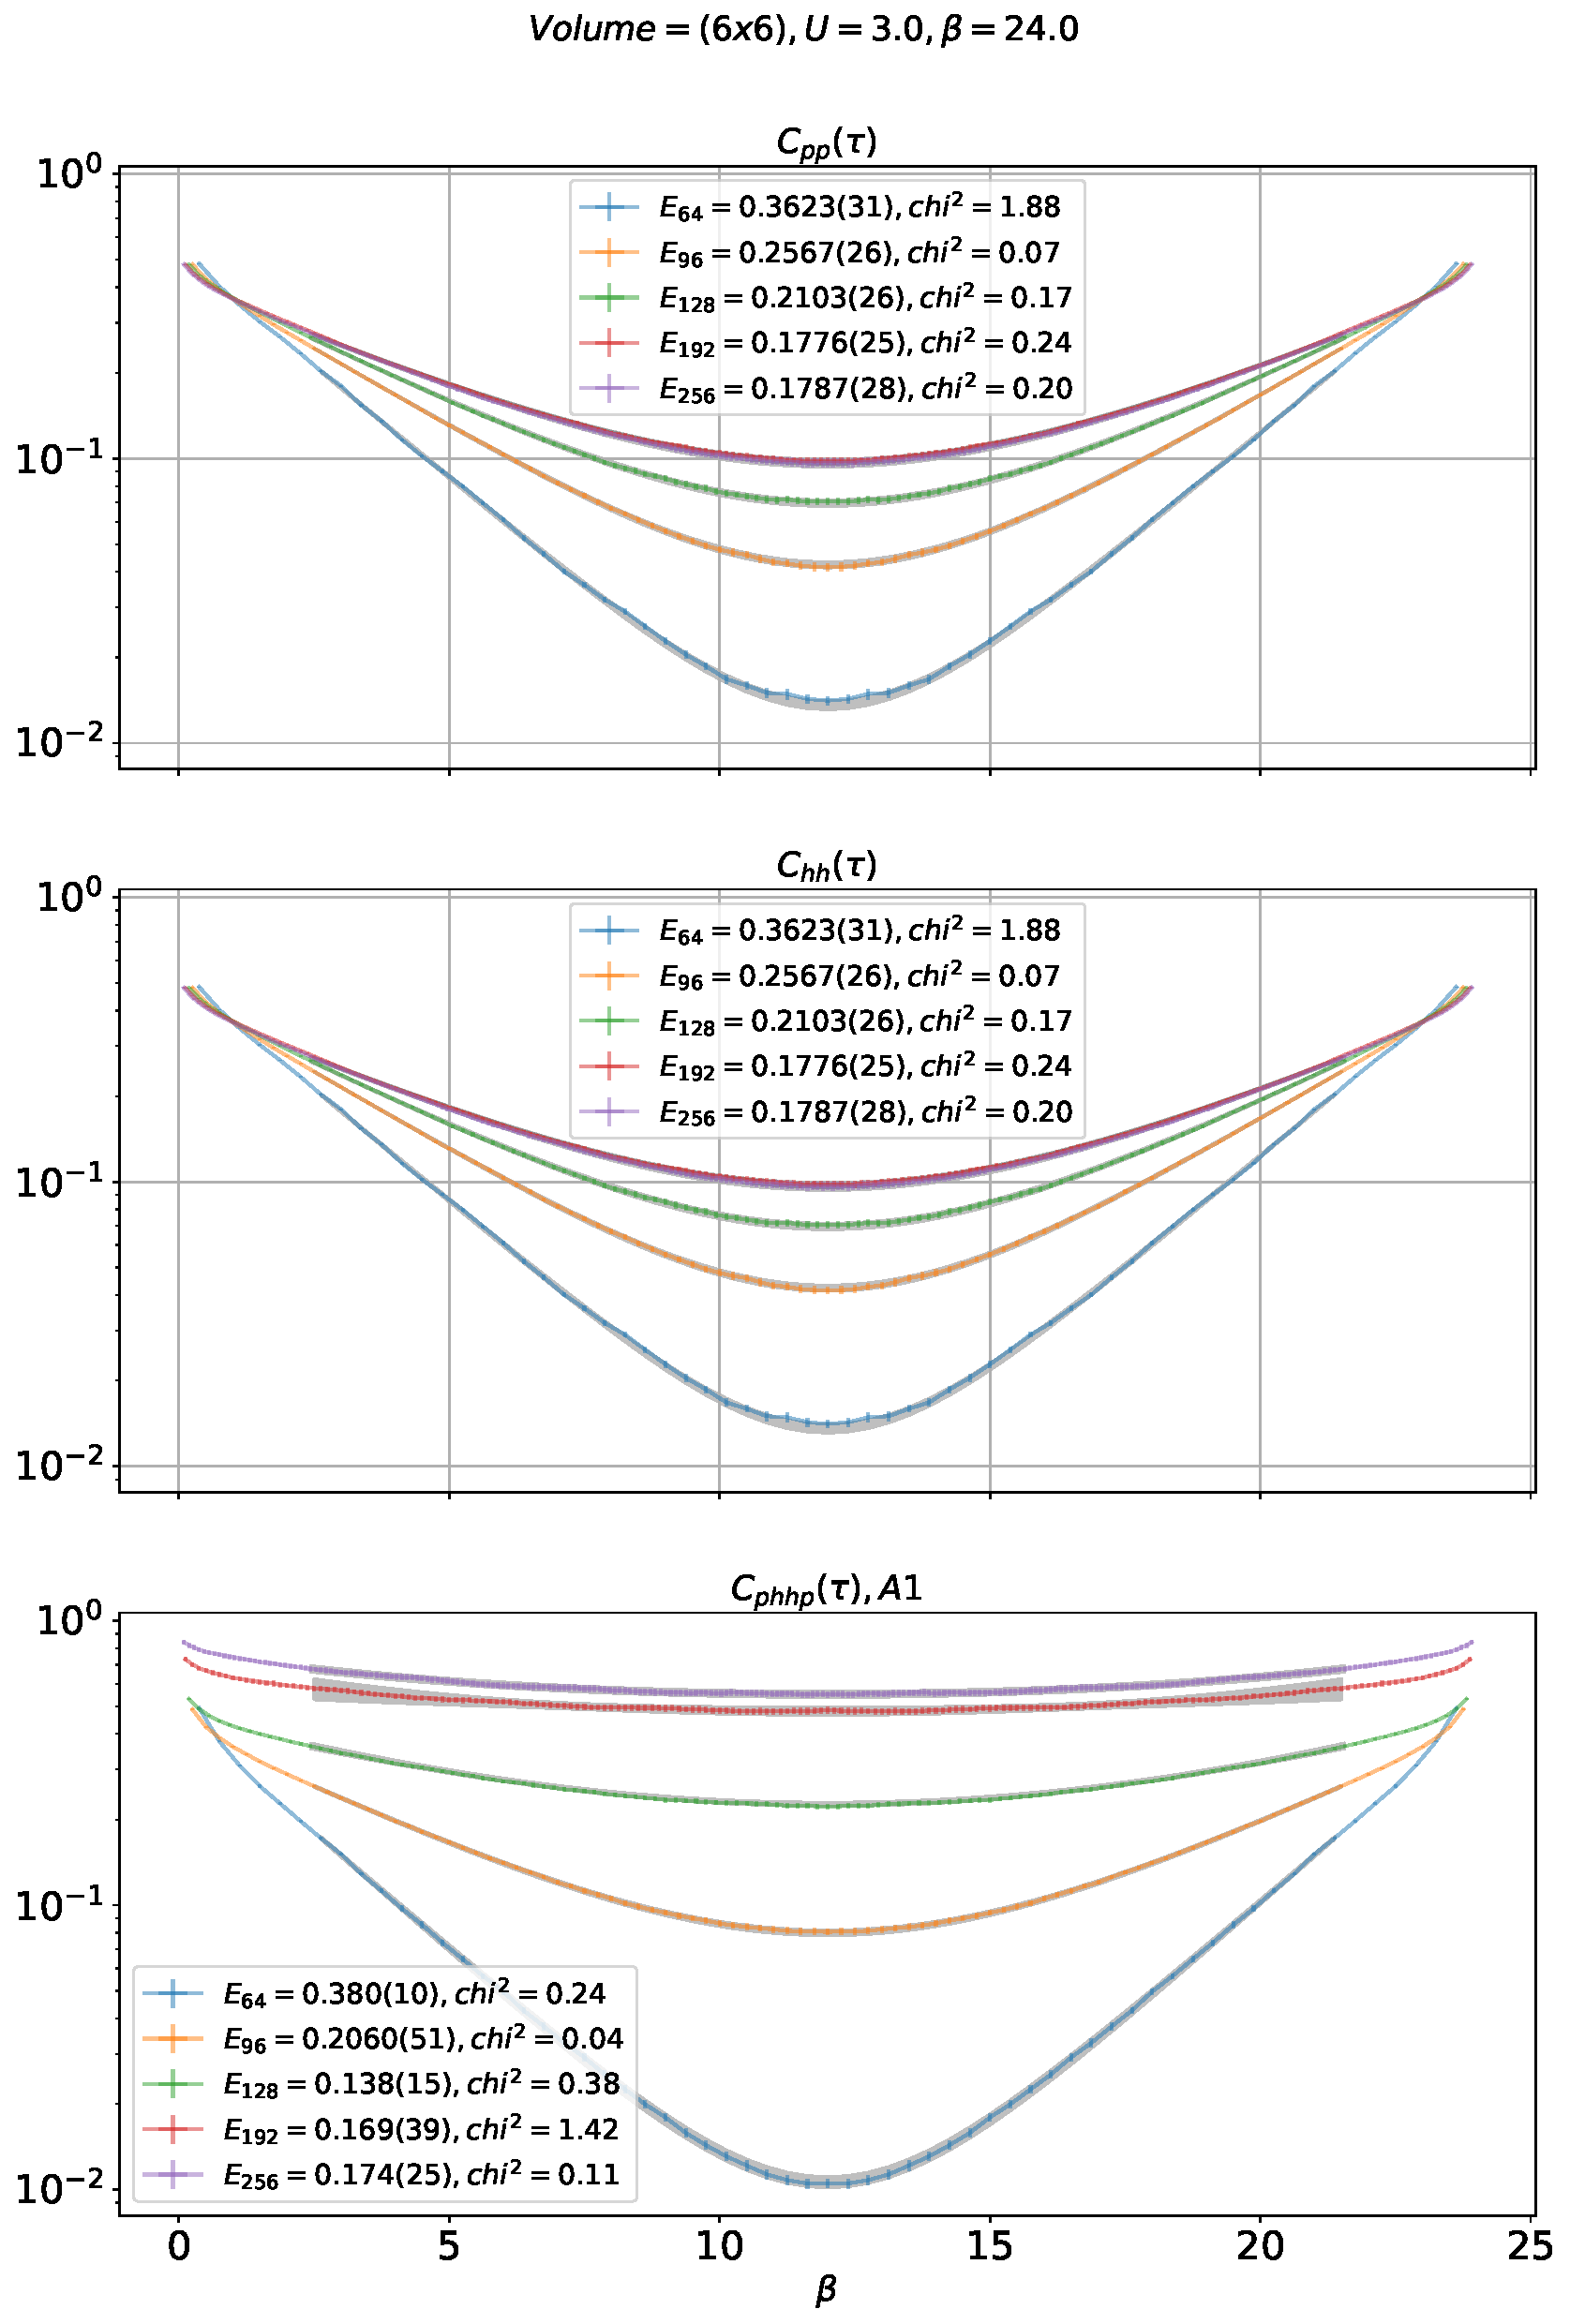
\includegraphics[width=\linewidth]{phhp-0-A1_6x6_U3.0_B24.0.pdf}
  \end{subfigure}%
  \begin{subfigure}{.5\textwidth}
    \centering
    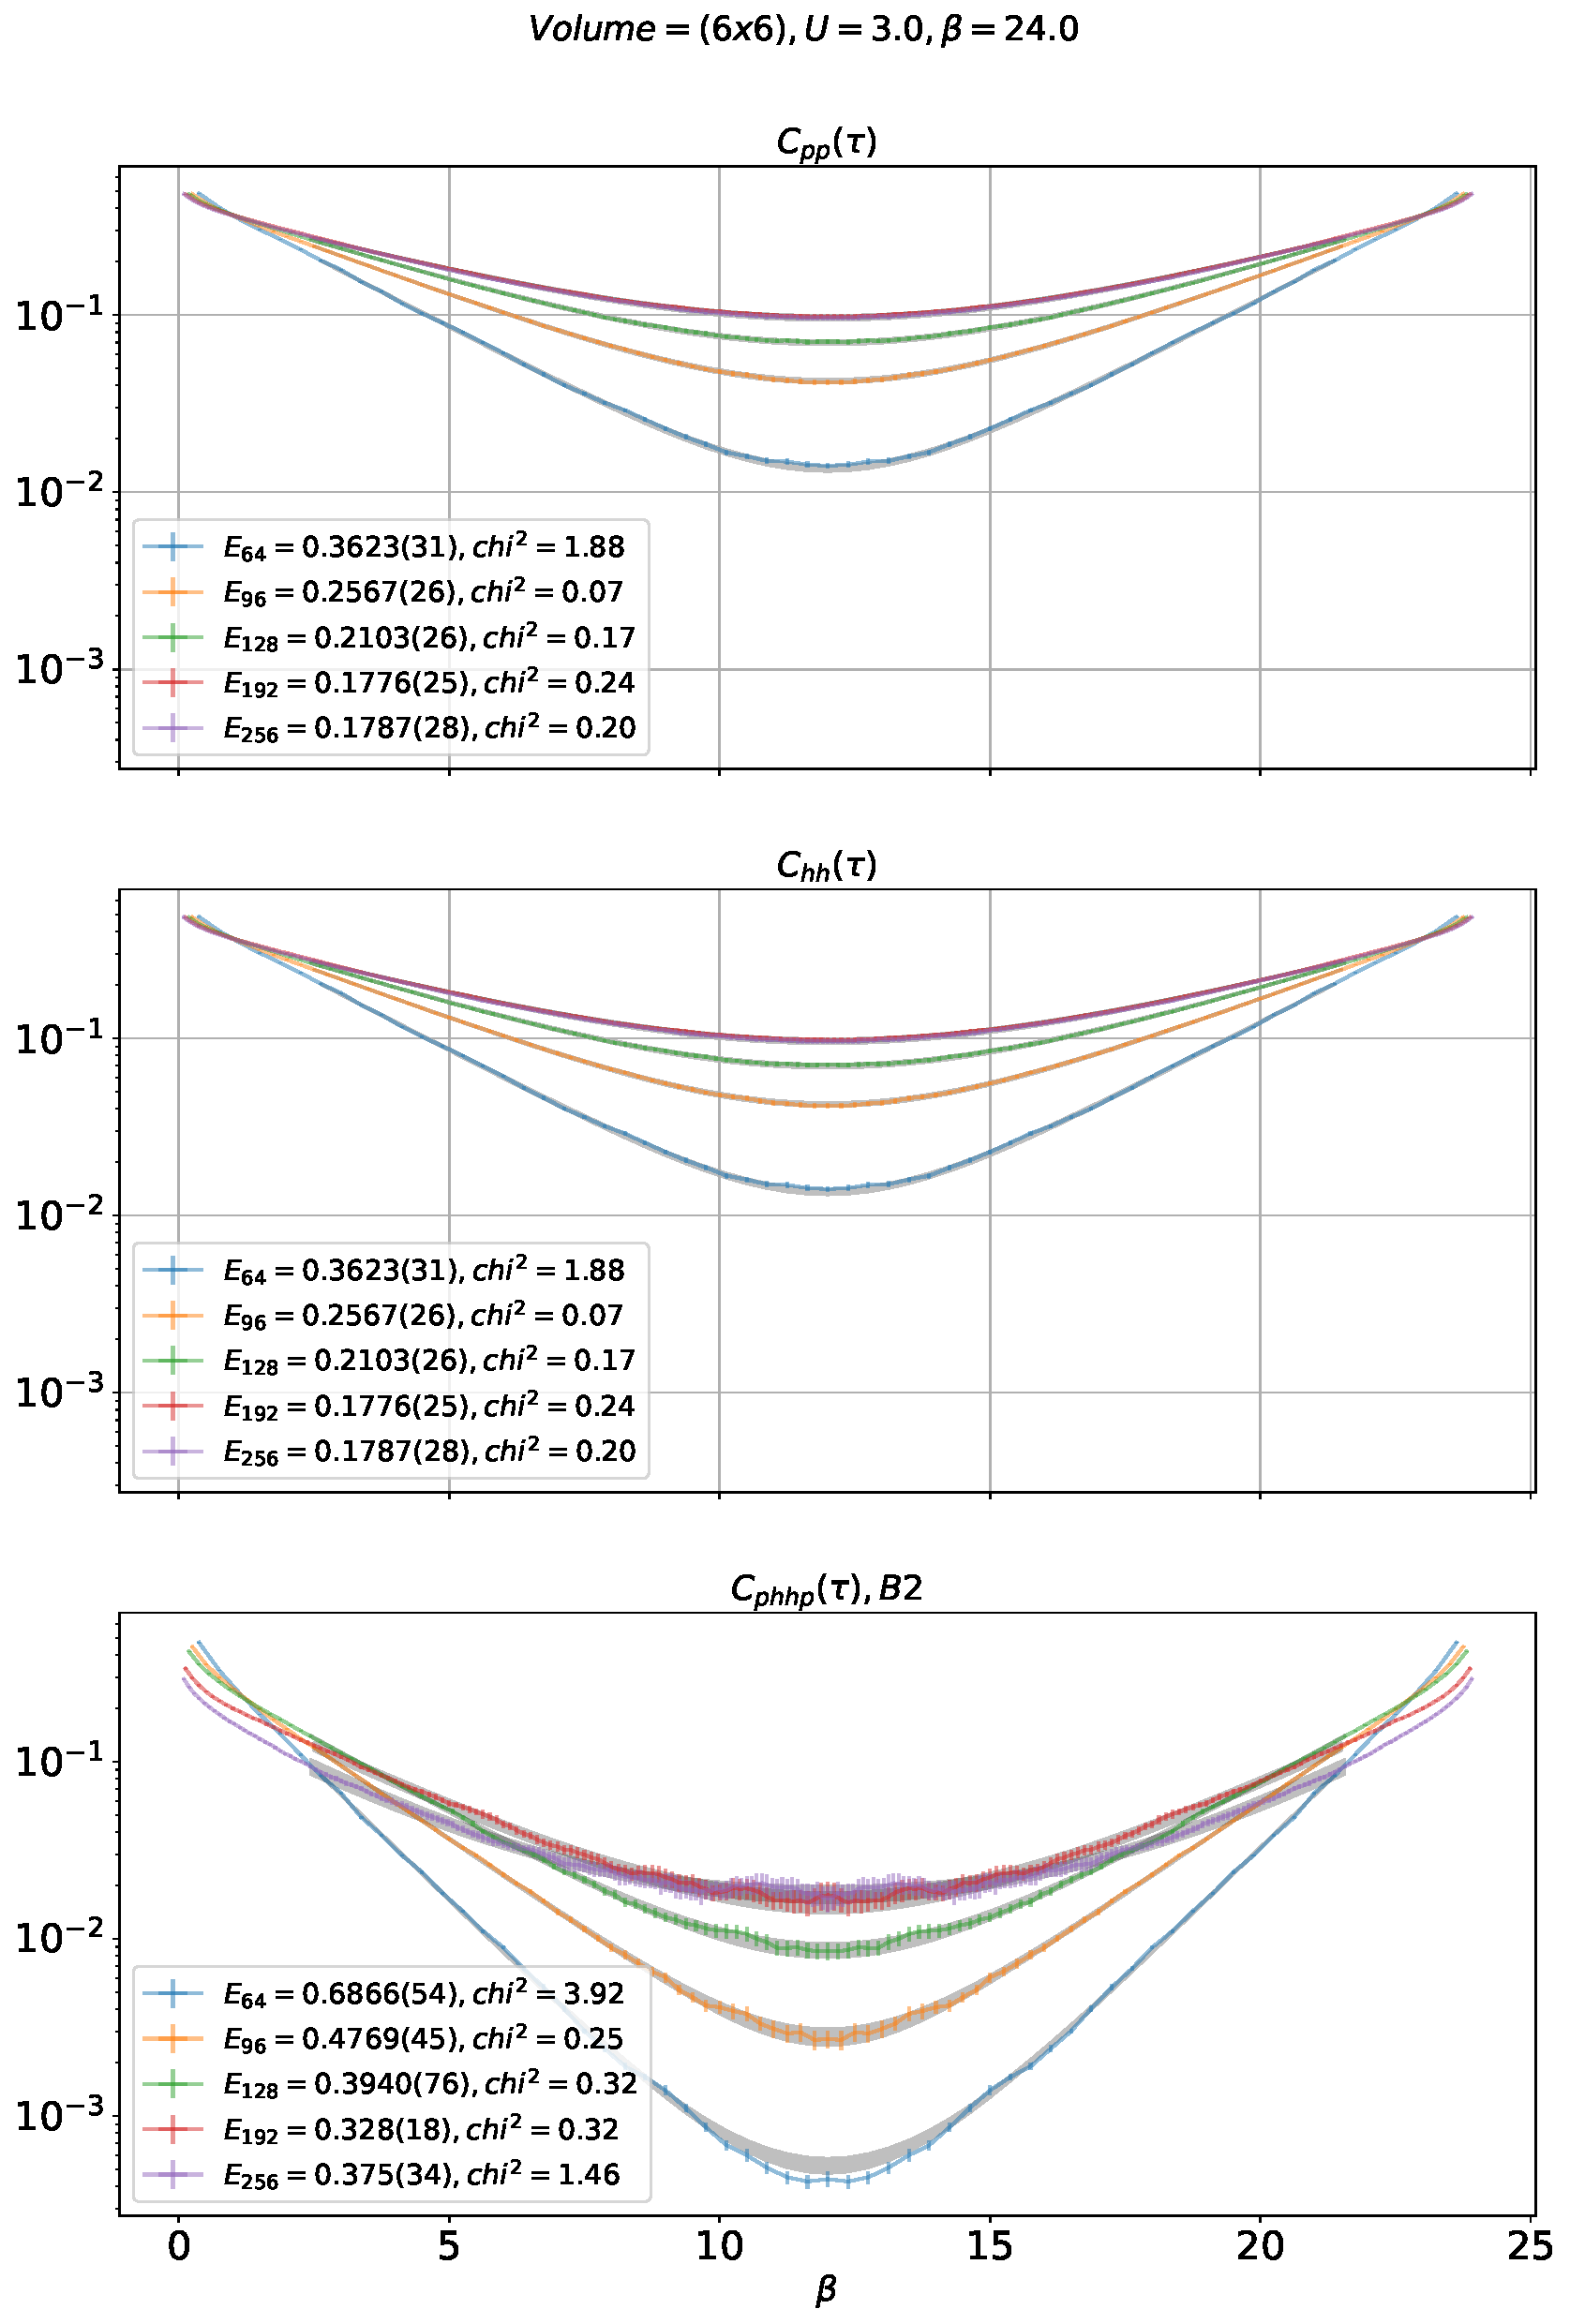
\includegraphics[width=\linewidth]{phhp-0-B2_6x6_U3.0_B24.0.pdf}
  \end{subfigure}
  \begin{subfigure}{.5\textwidth}
      \centering
      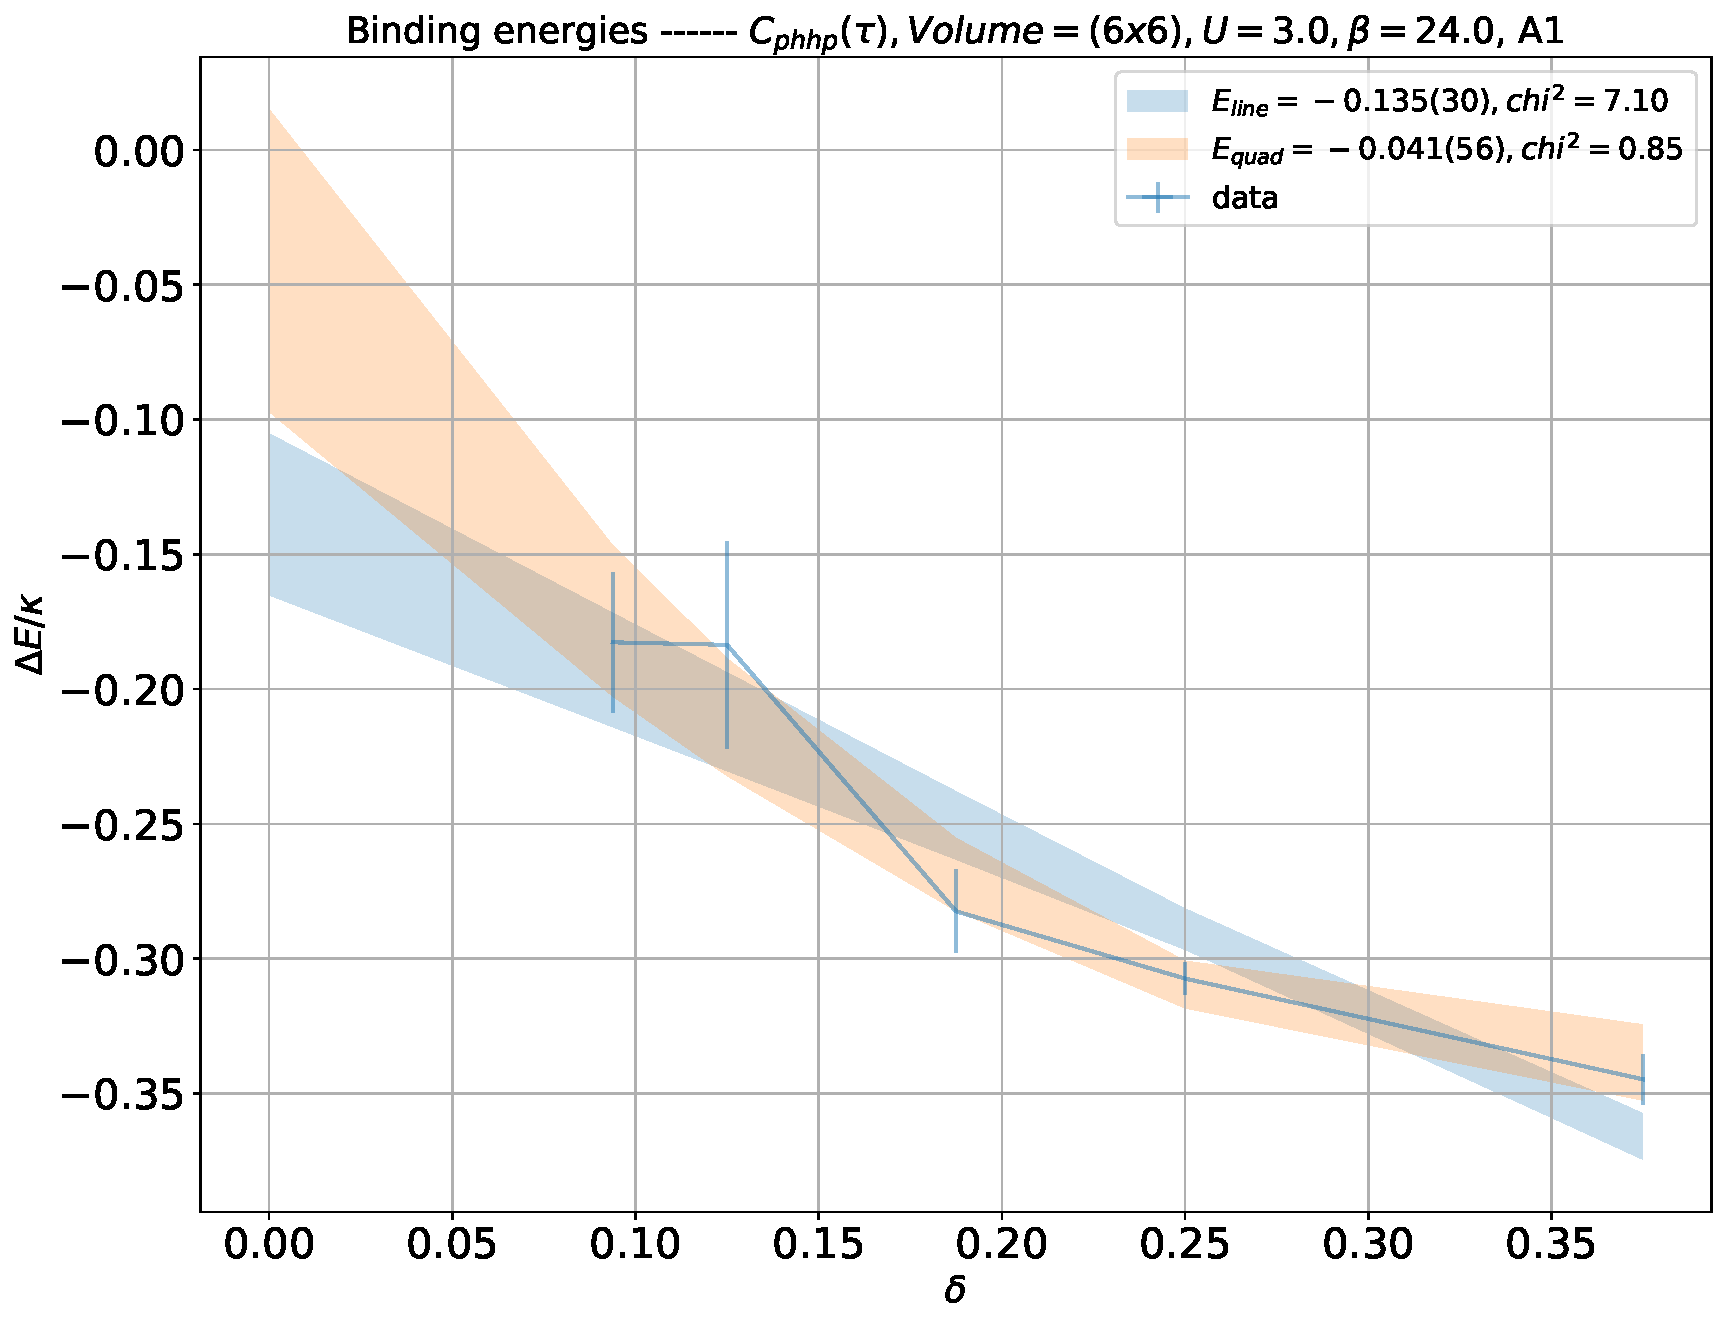
\includegraphics[width=\linewidth]{phhp-0-A1_6x6_U3.0_B24.0_cont.pdf}
  \end{subfigure}
  \begin{subfigure}{.5\textwidth}
      \centering
      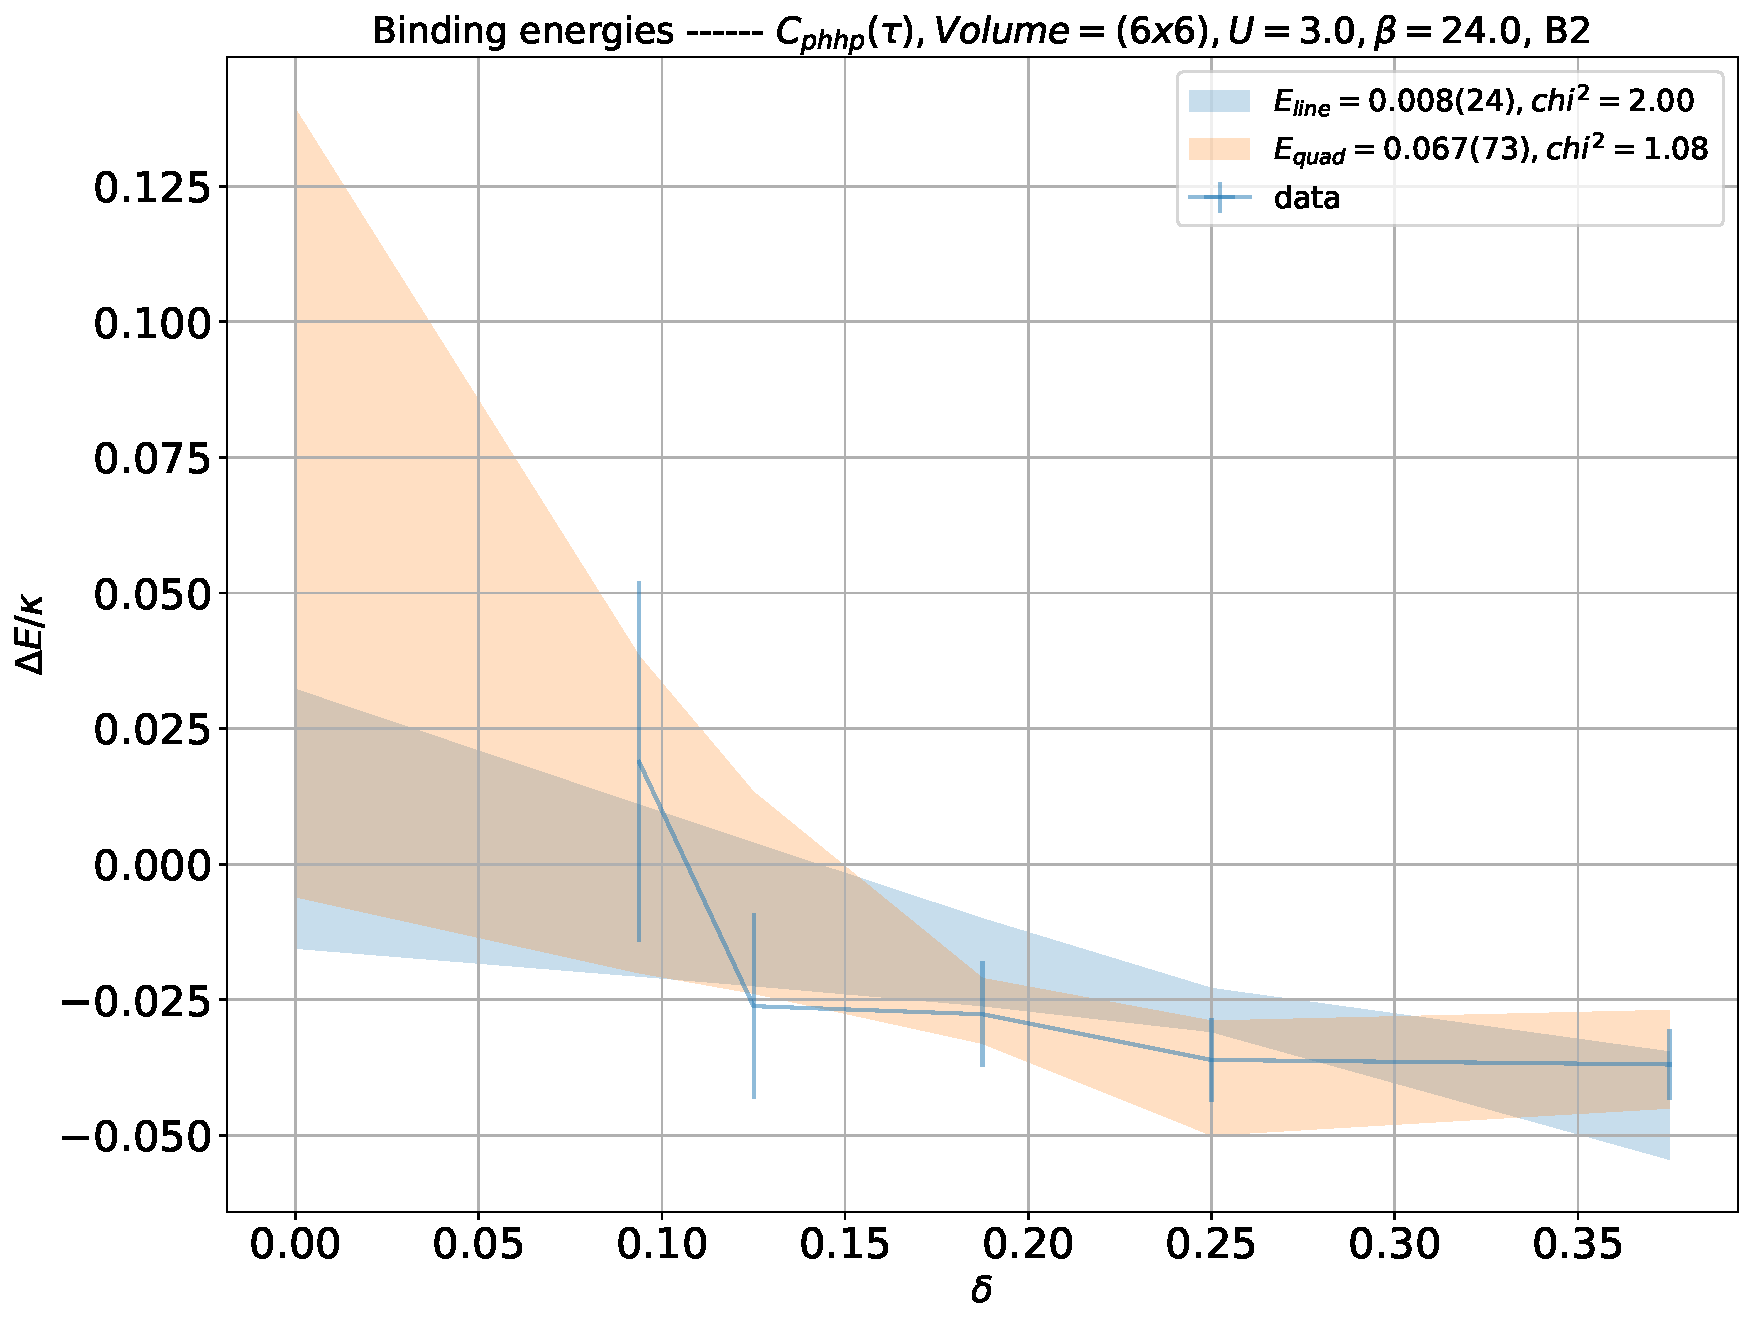
\includegraphics[width=\linewidth]{phhp-0-B2_6x6_U3.0_B24.0_cont.pdf}
  \end{subfigure}
  \caption{Binding energy extraction of the particle-hole pair at both irreducible representations, where we fit one- and two-body correlators for every $N_t$. This is followed by fitting a linear and a quadratic functions to the $\Delta E_{N_t}$ in order to extrapolate to the continuum limit ($N_t\to\infty$).}
  \label{fig:fig12}
\end{figure}

\begin{figure}
  \begin{subfigure}{.5\textwidth}
    \centering
    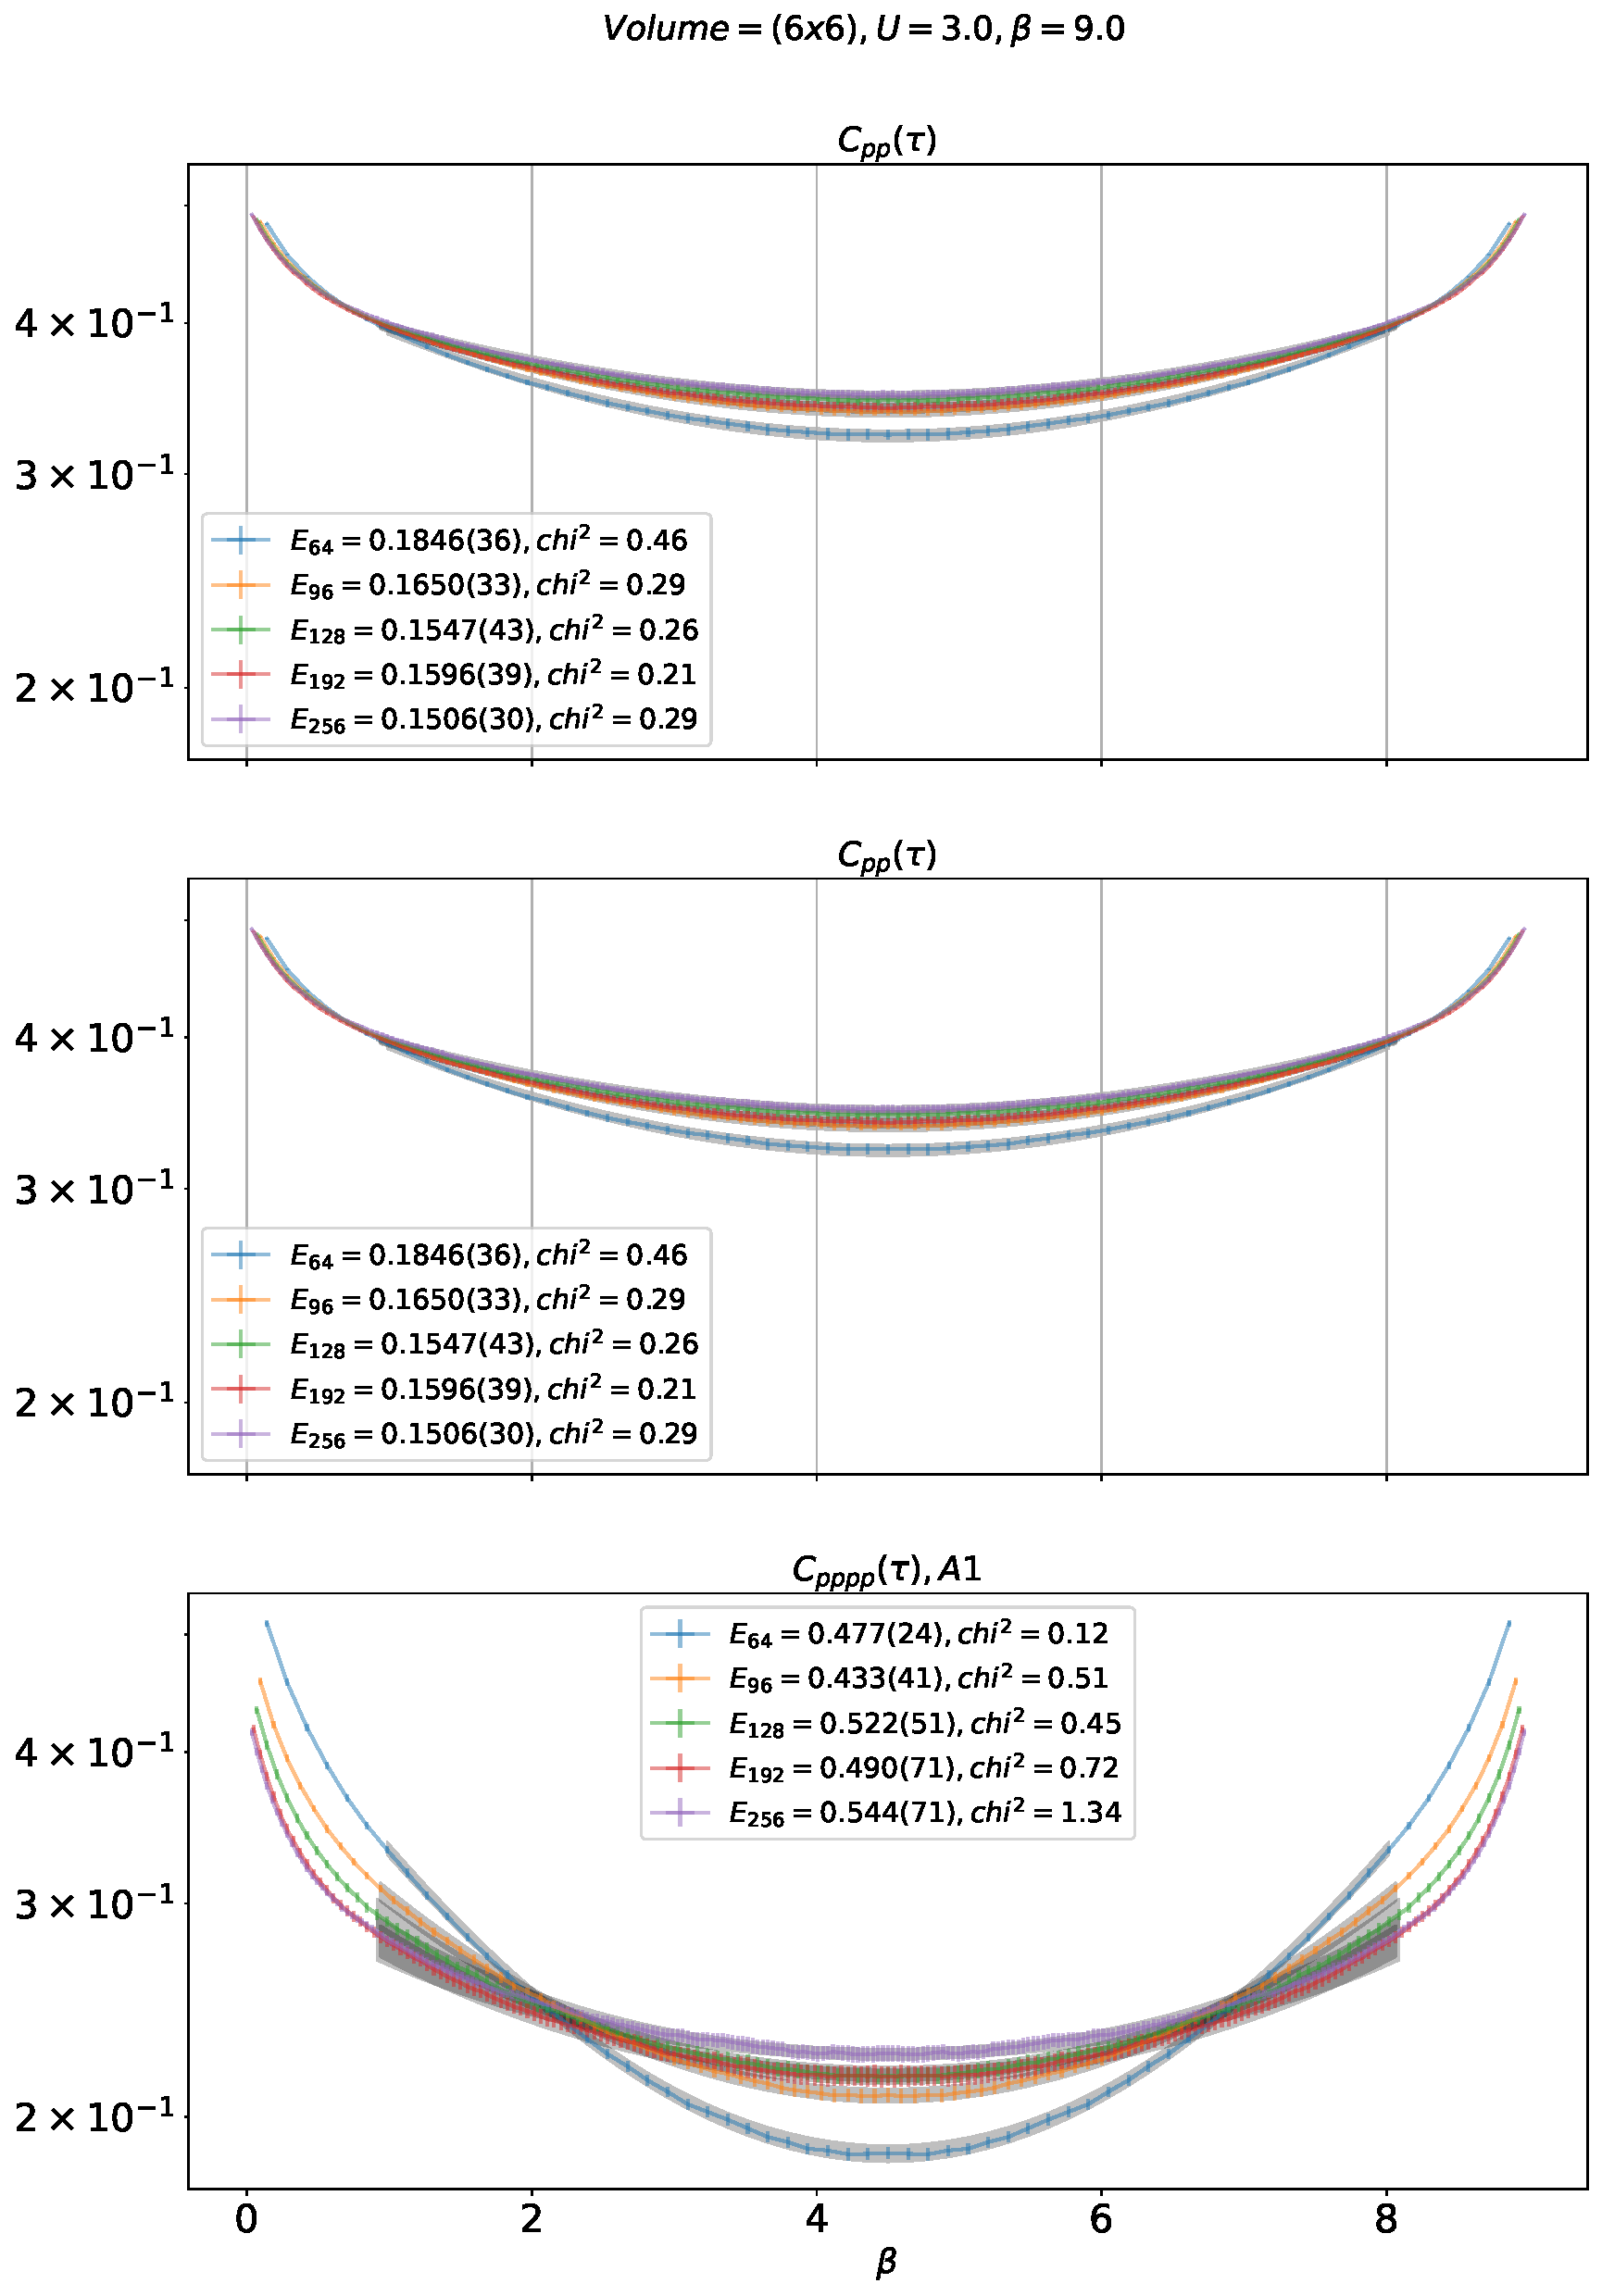
\includegraphics[width=\linewidth]{pppp-0-A1_6x6_U3.0_B9.0.pdf}
  \end{subfigure}%
  \begin{subfigure}{.5\textwidth}
    \centering
    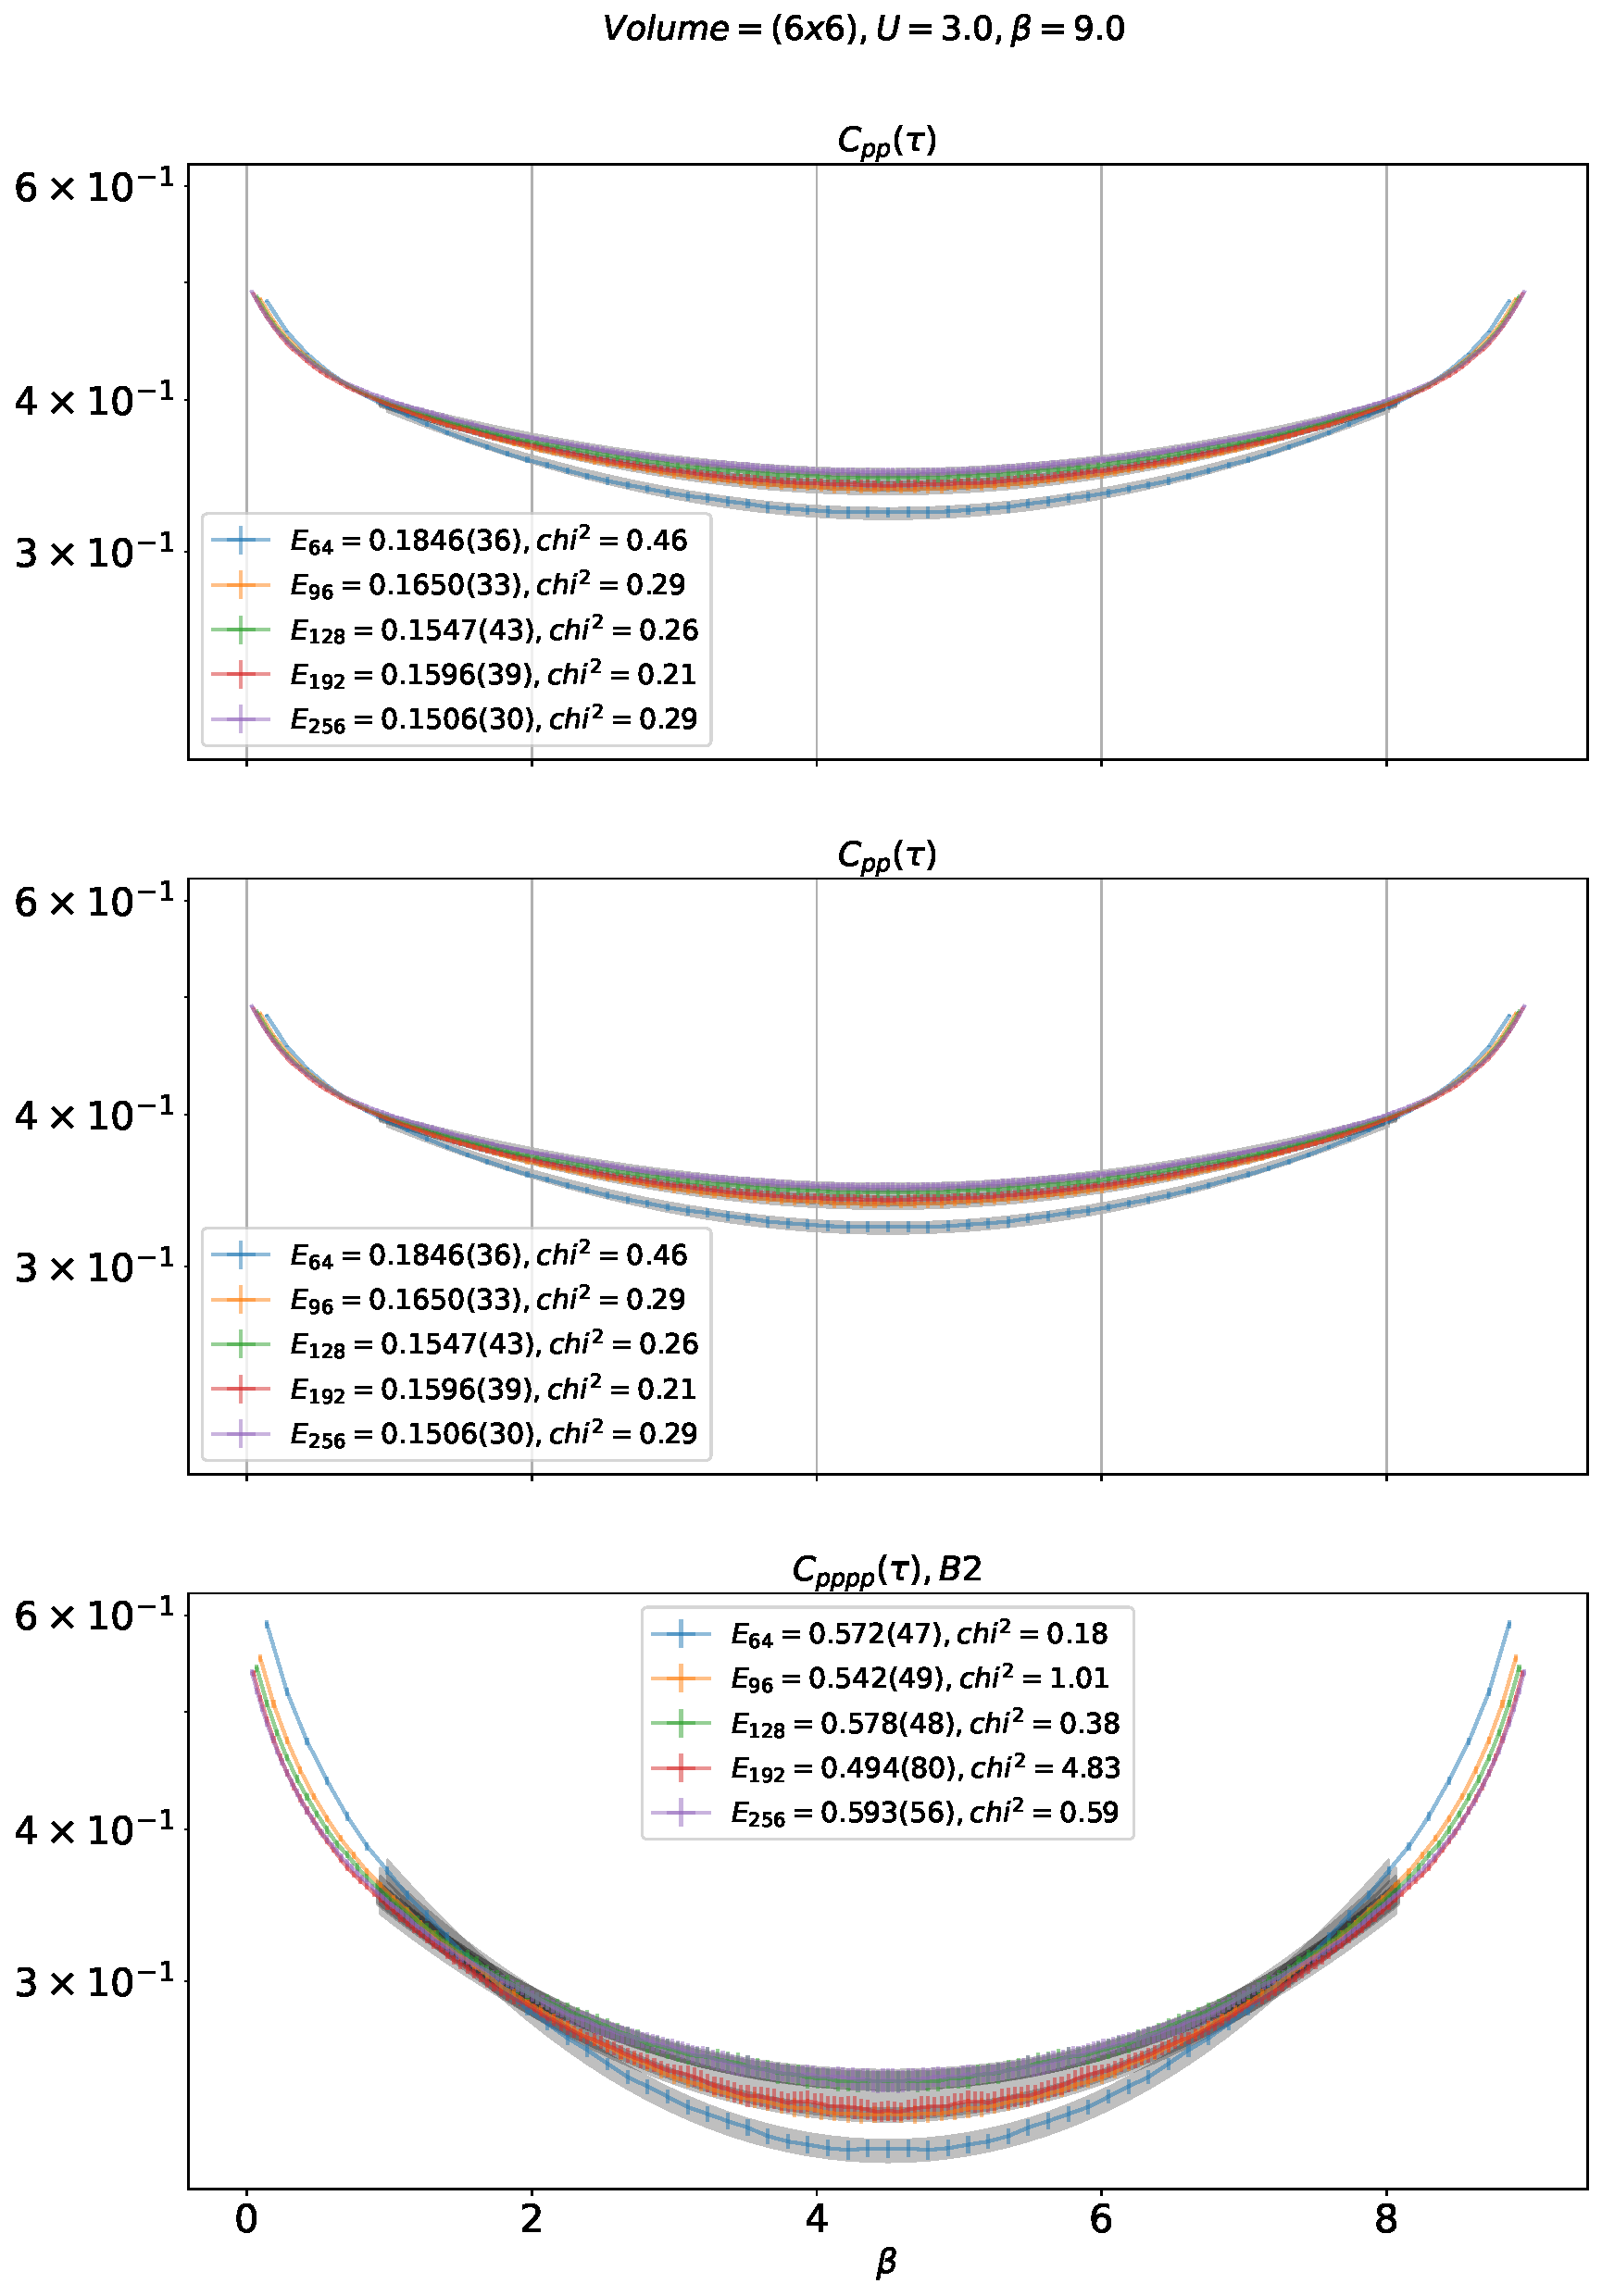
\includegraphics[width=\linewidth]{pppp-0-B2_6x6_U3.0_B9.0.pdf}
  \end{subfigure}
  \begin{subfigure}{.5\textwidth}
      \centering
      \includegraphics[width=\linewidth]{pppp-0-A1_6x6_U3.0_B9.0_cont.pdf}
  \end{subfigure}
  \begin{subfigure}{.5\textwidth}
      \centering
      \includegraphics[width=\linewidth]{pppp-0-B2_6x6_U3.0_B9.0_cont.pdf}
  \end{subfigure}
  \caption{Binding energy extraction of the particle-particle pair at both irreducible representations, where we fit one- and two-body correlators for every $N_t$. This is followed by fitting a linear and a quadratic functions to the $\Delta E_{N_t}$ in order to extrapolate to the continuum limit ($N_t\to\infty$).}
  \label{fig:fig13}
\end{figure}

\begin{figure}
  \begin{subfigure}{.5\textwidth}
    \centering
    \includegraphics[width=\linewidth]{pppp-0-A1_6x6_U3.0_B24.0.pdf}
  \end{subfigure}%
  \begin{subfigure}{.5\textwidth}
    \centering
    \includegraphics[width=\linewidth]{pppp-0-B2_6x6_U3.0_B24.0.pdf}
  \end{subfigure}
  \begin{subfigure}{.5\textwidth}
      \centering
      \includegraphics[width=\linewidth]{pppp-0-A1_6x6_U3.0_B24.0_cont.pdf}
  \end{subfigure}
  \begin{subfigure}{.5\textwidth}
      \centering
      \includegraphics[width=\linewidth]{pppp-0-B2_6x6_U3.0_B24.0_cont.pdf}
  \end{subfigure}
  \caption{Binding energy extraction of the particle-particle pair at both irreducible representations, where we fit one- and two-body correlators for every $N_t$. This is followed by fitting a linear and a quadratic functions to the $\Delta E_{N_t}$ in order to extrapolate to the continuum limit ($N_t\to\infty$).}
  \label{fig:fig14}
\end{figure}

\begin{figure}
  \begin{subfigure}{.5\textwidth}
    \centering
    \includegraphics[width=\linewidth]{phhp-0-A1_6x6_U4.0_B6.0.pdf}
  \end{subfigure}%
  \begin{subfigure}{.5\textwidth}
    \centering
    \includegraphics[width=\linewidth]{phhp-0-B2_6x6_U4.0_B6.0.pdf}
  \end{subfigure}
  \begin{subfigure}{.5\textwidth}
      \centering
      \includegraphics[width=\linewidth]{phhp-0-A1_6x6_U4.0_B6.0_cont.pdf}
  \end{subfigure}
  \begin{subfigure}{.5\textwidth}
      \centering
      \includegraphics[width=\linewidth]{phhp-0-B2_6x6_U4.0_B6.0_cont.pdf}
  \end{subfigure}
  \caption{Binding energy extraction of the particle-hole pair at both irreducible representations, where we fit one- and two-body correlators for every $N_t$. This is followed by fitting a linear and a quadratic functions to the $\Delta E_{N_t}$ in order to extrapolate to the continuum limit ($N_t\to\infty$).}
  \label{fig:fig15}
\end{figure}

\begin{figure}
  \begin{subfigure}{.5\textwidth}
    \centering
    \includegraphics[width=\linewidth]{phhp-0-A1_6x6_U4.0_B9.0.pdf}
  \end{subfigure}%
  \begin{subfigure}{.5\textwidth}
    \centering
    \includegraphics[width=\linewidth]{phhp-0-B2_6x6_U4.0_B9.0.pdf}
  \end{subfigure}
  \begin{subfigure}{.5\textwidth}
      \centering
      \includegraphics[width=\linewidth]{phhp-0-A1_6x6_U4.0_B9.0_cont.pdf}
  \end{subfigure}
  \begin{subfigure}{.5\textwidth}
      \centering
      \includegraphics[width=\linewidth]{phhp-0-B2_6x6_U4.0_B9.0_cont.pdf}
  \end{subfigure}
  \caption{Binding energy extraction of the particle-hole pair at both irreducible representations, where we fit one- and two-body correlators for every $N_t$. This is followed by fitting a linear and a quadratic functions to the $\Delta E_{N_t}$ in order to extrapolate to the continuum limit ($N_t\to\infty$).}
  \label{fig:fig16}
\end{figure}

\begin{figure}
  \begin{subfigure}{.5\textwidth}
    \centering
    \includegraphics[width=\linewidth]{phhp-0-A1_6x6_U4.0_B24.0.pdf}
  \end{subfigure}%
  \begin{subfigure}{.5\textwidth}
    \centering
    \includegraphics[width=\linewidth]{phhp-0-B2_6x6_U4.0_B24.0.pdf}
  \end{subfigure}
  \begin{subfigure}{.5\textwidth}
      \centering
      \includegraphics[width=\linewidth]{phhp-0-A1_6x6_U4.0_B24.0_cont.pdf}
  \end{subfigure}
  \begin{subfigure}{.5\textwidth}
      \centering
      \includegraphics[width=\linewidth]{phhp-0-B2_6x6_U4.0_B24.0_cont.pdf}
  \end{subfigure}
  \caption{Binding energy extraction of the particle-hole pair at both irreducible representations, where we fit one- and two-body correlators for every $N_t$. This is followed by fitting a linear and a quadratic functions to the $\Delta E_{N_t}$ in order to extrapolate to the continuum limit ($N_t\to\infty$).}
  \label{fig:fig17}
\end{figure}

\begin{figure}
  \begin{subfigure}{.5\textwidth}
    \centering
    \includegraphics[width=\linewidth]{pppp-0-A1_6x6_U4.0_B6.0.pdf}
  \end{subfigure}%
  \begin{subfigure}{.5\textwidth}
    \centering
    \includegraphics[width=\linewidth]{pppp-0-B2_6x6_U4.0_B6.0.pdf}
  \end{subfigure}
  \begin{subfigure}{.5\textwidth}
      \centering
      \includegraphics[width=\linewidth]{pppp-0-A1_6x6_U4.0_B6.0_cont.pdf}
  \end{subfigure}
  \begin{subfigure}{.5\textwidth}
      \centering
      \includegraphics[width=\linewidth]{pppp-0-B2_6x6_U4.0_B6.0_cont.pdf}
  \end{subfigure}
  \caption{Binding energy extraction of the particle-particle pair at both irreducible representations, where we fit one- and two-body correlators for every $N_t$. This is followed by fitting a linear and a quadratic functions to the $\Delta E_{N_t}$ in order to extrapolate to the continuum limit ($N_t\to\infty$).}
  \label{fig:fig18}
\end{figure}

\begin{figure}
  \begin{subfigure}{.5\textwidth}
    \centering
    \includegraphics[width=\linewidth]{pppp-0-A1_6x6_U4.0_B9.0.pdf}
  \end{subfigure}%
  \begin{subfigure}{.5\textwidth}
    \centering
    \includegraphics[width=\linewidth]{pppp-0-B2_6x6_U4.0_B9.0.pdf}
  \end{subfigure}
  \begin{subfigure}{.5\textwidth}
      \centering
      \includegraphics[width=\linewidth]{pppp-0-A1_6x6_U4.0_B9.0_cont.pdf}
  \end{subfigure}
  \begin{subfigure}{.5\textwidth}
      \centering
      \includegraphics[width=\linewidth]{pppp-0-B2_6x6_U4.0_B9.0_cont.pdf}
  \end{subfigure}
  \caption{Binding energy extraction of the particle-particle pair at both irreducible representations, where we fit one- and two-body correlators for every $N_t$. This is followed by fitting a linear and a quadratic functions to the $\Delta E_{N_t}$ in order to extrapolate to the continuum limit ($N_t\to\infty$).}
  \label{fig:fig19}
\end{figure}

\begin{figure}
  \begin{subfigure}{.5\textwidth}
    \centering
    \includegraphics[width=\linewidth]{pppp-0-A1_6x6_U4.0_B24.0.pdf}
  \end{subfigure}%
  \begin{subfigure}{.5\textwidth}
    \centering
    \includegraphics[width=\linewidth]{pppp-0-B2_6x6_U4.0_B24.0.pdf}
  \end{subfigure}
  \begin{subfigure}{.5\textwidth}
      \centering
      \includegraphics[width=\linewidth]{pppp-0-A1_6x6_U4.0_B24.0_cont.pdf}
  \end{subfigure}
  \begin{subfigure}{.5\textwidth}
      \centering
      \includegraphics[width=\linewidth]{pppp-0-B2_6x6_U4.0_B24.0_cont.pdf}
  \end{subfigure}
  \caption{Binding energy extraction of the particle-particle pair at both irreducible representations, where we fit one- and two-body correlators for every $N_t$. This is followed by fitting a linear and a quadratic functions to the $\Delta E_{N_t}$ in order to extrapolate to the continuum limit ($N_t\to\infty$).}
  \label{fig:fig20}
\end{figure}

%The \LaTeX\ WikiBook~\cite{latexwiki} is a useful source of information on \LaTeX.

\printbibliography[heading=subbibliography]

%------------------------------------------------------------------------------
% Include the following lines and comment out \printbibliography if
% you use BiBTeX for the bibliography.
% If you use biblatex package the files should be specified in the preamble.
% \KOMAoptions{toc=bibliography}
% {\raggedright
%   \bibliographystyle{../refs/atlasBibStyleWithTitle.bst}
%   % \bibliographystyle{unsrt}
%   \bibliography{./thesis_refs,../refs/standard_refs-bibtex}
% }

%------------------------------------------------------------------------------
% Declare lists of figures and tables and acknowledgements as backmatter
% Chapter/section numbers are turned off
\backmatter

\listoffigures
\listoftables

%------------------------------------------------------------------------------
% Print the glossary and list of acronyms
% \printglossaries

%------------------------------------------------------------------------------
% You could instead add your acknowledgements here - don't forget to
% also add them to \includeonly above
% %------------------------------------------------------------------------------
\chapter*{Acknowledgements}
\label{sec:ack}
%------------------------------------------------------------------------------

I would like to thank first and foremost my supervisors Prof. Dr. Stefan Krieg and Prof. Dr. Thomas Luu who introduced me into the field of Computational Physics. They gave me the incredible opportunity to work with them at Forschungszentrum Jülich on this project. 

I am extremely grateful to Dr. Evan Berkowitz, with whom I was closely working. His guidance and continuous support helped me throughout my master's thesis. I am also grateful for the excellent notes that Evan provided, which laid the groundwork for my thesis.

Special thanks to my colleagues Keshvi, Christoph, Johann, Nico, and Marcel for the ideas and suggestions in the meetings throughout the year. Especially Aleksandra Salkina who supported me throughout my whole Master's study. I also sincerely acknowledge the computing time granted through JARA on the supercomputer JURECA at Forschungszentrum Jülich.

% You should probably use \texttt{\textbackslash chapter*} for
% acknowledgements at the beginning of a thesis and
% \texttt{\textbackslash chapter} for the end.

%%% Local Variables: 
%%% mode: latex
%%% TeX-master: "../mythesis"
%%% End: 


%------------------------------------------------------------------------------
% CV needed when you submit your PhD thesis
% \definecolor{lightgray}{gray}{0.8}
\newcolumntype{L}{>{\raggedleft}p{0.15\textwidth}}
\newcolumntype{R}{p{0.8\textwidth}}
\newcommand\VRule{\color{lightgray}\vrule width 0.5pt}

\thispagestyle{empty}
\section*{Curriculum Vitae}

\subsection*{Personal Details}

\begin{tabular}{L!{\VRule}R}
Name & Johann Schmidt \\
Date of Birth &  \\
Email & abc@physik.uni-def.de \\
Family status & Single
\end{tabular}

\subsection*{Education}

\begin{tabular}{L!{\VRule}R}
1997--2003 & Abitur, ABC Secondary School, Hamburg, Germany\\
2004--2007 & BSc in Physics, Rheinische Friedrich-Wilhelms-Universität, Bonn, Germany.\\
2006 & CERN Summer Student, Geneva, Switzerland. \\
2007--2009 &  MSc in Physics Rheinische Friedrich-Wilhelms-Universität, Bonn, Germany. \\
2009--2012 &  PhD in Physics, Rheinische Friedrich-Wilhelms-Universität, Bonn, Germany. \\
2012 & Advanced Data Analysis School, Frankfurt, Germany.
\end{tabular}

\subsection*{Professional Experience}

\begin{tabular}{L!{\VRule}R}
2004 & Summer Student at CERN, Geneva, Switzerland. \\
2007--2012 & Doctoral work at the University of Bonn, Germany. \\
2008--2009 & Fieldwork at CERN, Geneva, Switzerland.\\
2011 & Talk at the Advanced Physics Conference, Timbucto
\end{tabular}

\subsection*{Languages}
\begin{tabular}{L!{\VRule}R}
German & Mother tongue \\
English & Fluent \\
Russian & Basic
\end{tabular}


\end{document}
